%%%%%%%%%%%%%%%%%%%%%%%%%%%%%%%%%%%%%%%%%
% Masters/Doctoral Thesis 
% LaTeX Template
% Version 1.43 (17/5/14)
%
% This template has been downloaded from:
% http://www.LaTeXTemplates.com
%
% Original authors:
% Steven Gunn 
% http://users.ecs.soton.ac.uk/srg/softwaretools/document/templates/
% and
% Sunil Patel
% http://www.sunilpatel.co.uk/thesis-template/
%
% License:
% CC BY-NC-SA 3.0 (http://creativecommons.org/licenses/by-nc-sa/3.0/)
%
% Note:
% Make sure to edit document variables in the Thesis.cls file
%
%%%%%%%%%%%%%%%%%%%%%%%%%%%%%%%%%%%%%%%%%

%----------------------------------------------------------------------------------------
%	PACKAGES AND OTHER DOCUMENT CONFIGURATIONS
%----------------------------------------------------------------------------------------

\documentclass[11pt, oneside]{Thesis} % The default font size and one-sided printing (no margin offsets)

\graphicspath{{Pictures/}} % Specifies the directory where pictures are stored

\usepackage[square, numbers, comma, sort&compress]{natbib} % Use the natbib reference package - read up on this to edit the reference style; if you want text (e.g. Smith et al., 2012) for the in-text references (instead of numbers), remove 'numbers' 
\hypersetup{urlcolor=blue, colorlinks=true} % Colors hyperlinks in blue - change to black if annoying
\usepackage{amssymb}
\usepackage{morefloats}
\usepackage{amsmath}
\usepackage{amsfonts}
\usepackage{lastpage}
\usepackage{multirow}
\usepackage{epstopdf}
\usepackage{graphicx}
\usepackage{caption}
%\usepackage{titlesec}
%\usepackage{subfig}
\usepackage{siunitx}
\usepackage{chngcntr}
\usepackage{wasysym}
\usepackage{pifont}
\usepackage{amsfonts}
\usepackage{caption}
\usepackage{subcaption}
\usepackage{pifont}
\captionsetup[sub]{labelsep=newline}
\usepackage{fancyhdr}
\pagestyle{fancy}
\usepackage{tikz}
\usetikzlibrary{fit,calc,positioning,decorations.pathreplacing,matrix}
\usepackage{pgflibraryarrows}
\usepackage{pgflibrarysnakes}
\usepackage{pgfplots}
\pgfplotsset{compat=newest}

%\pgfplotsset{pgfplots,compat=newest}
%\usepackage[usenames,dvipsnames]{color}
\definecolor{light-gray}{gray}{0.75}

%\usepackage{amsmath}
%\usepackage{subcaption}
%% The amsthm package provides extended theorem environments
%% \usepackage{amsthm}
\fancyhf{}
\title{\ttitle} % Defines the thesis title - don't touch this

\begin{document}

\frontmatter % Use roman page numbering style (i, ii, iii, iv...) for the pre-content pages

\setstretch{1.3} % Line spacing of 1.3

% Define the page headers using the FancyHdr package and set up for one-sided printing
\fancyhead{} % Clears all page headers and footers
\rhead{\thepage} % Sets the right side header to show the page number
\lhead{} % Clears the left side page header

\pagestyle{fancy} % Finally, use the "fancy" page style to implement the FancyHdr headers

\newcommand{\HRule}{\rule{\linewidth}{0.5mm}} % New command to make the lines in the title page

% PDF meta-data
\hypersetup{pdftitle={\ttitle}}
\hypersetup{pdfsubject=\subjectname}
\hypersetup{pdfauthor=\authornames}
\hypersetup{pdfkeywords=\keywordnames}

%----------------------------------------------------------------------------------------
%	TITLE PAGE
%----------------------------------------------------------------------------------------

\begin{titlepage}
\begin{center}

\textsc{\LARGE \univname}\\[1.5cm] % University name
\textsc{\Large Doctoral Thesis}\\[0.5cm] % Thesis type

\HRule \\[0.4cm] % Horizontal line
{\huge \bfseries \ttitle}\\[0.4cm] % Thesis title
\HRule \\[1.5cm] % Horizontal line
 
\begin{minipage}{0.4\textwidth}
\begin{flushleft} \large
\emph{Author:}\\
{\authornames} % Author name - remove the \href bracket to remove the link
\end{flushleft}
\end{minipage}
\begin{minipage}{0.4\textwidth}
\begin{flushright} \large
\emph{Supervisor:} \\
\href{http://isim.asu.edu/}{\supname} % Supervisor name - remove the \href bracket to remove the link  
\end{flushright}
\end{minipage}\\[3cm]
 
\large \textit{A thesis submitted in fulfilment of the requirements\\ for the degree of \degreename}\\[0.3cm] % University requirement text
\textit{in the}\\[0.4cm]
\groupname\\\deptname\\[2cm] % Research group name and department name

\includegraphics[width=4cm]{logo} \par % University/department logo - uncomment to place it 
{\Large \today}\\[4cm] % Date
 
\vfill
\end{center}

\end{titlepage}

%----------------------------------------------------------------------------------------
%	DECLARATION PAGE
%	Your institution may give you a different text to place here
%----------------------------------------------------------------------------------------

\Declaration{

\addtocontents{toc}{\vspace{1em}} % Add a gap in the Contents, for aesthetics

I, \authornames, declare that this thesis titled, '\ttitle' and the work presented in it are my own. I confirm that:

\begin{itemize} 
\item[\tiny{$\blacksquare$}] This work was done wholly or mainly while in candidature for a research degree at this University.
\item[\tiny{$\blacksquare$}] Where any part of this thesis has previously been submitted for a degree or any other qualification at this University or any other institution, this has been clearly stated.
\item[\tiny{$\blacksquare$}] Where I have consulted the published work of others, this is always clearly attributed.
\item[\tiny{$\blacksquare$}] Where I have quoted from the work of others, the source is always given. With the exception of such quotations, this thesis is entirely my own work.
\item[\tiny{$\blacksquare$}] I have acknowledged all main sources of help.
\item[\tiny{$\blacksquare$}] Where the thesis is based on work done by myself jointly with others, I have made clear exactly what was done by others and what I have contributed myself.\\
\end{itemize}
 
Signed:\\
\rule[1em]{25em}{0.5pt} % This prints a line for the signature
 
Date:\\
\rule[1em]{25em}{0.5pt} % This prints a line to write the date
}

\clearpage % Start a new page

%----------------------------------------------------------------------------------------
%	QUOTATION PAGE
%----------------------------------------------------------------------------------------

\pagestyle{empty} % No headers or footers for the following pages

\null\vfill % Add some space to move the quote down the page a bit

\textit{``Thanks to my solid academic training, today I can write hundreds of words on virtually any topic without possessing a shred of information, which is how I got a good job in journalism."}

\begin{flushright}
Dave Barry
\end{flushright}

\vfill\vfill\vfill\vfill\vfill\vfill\null % Add some space at the bottom to position the quote just right

\clearpage % Start a new page

%----------------------------------------------------------------------------------------
%	ABSTRACT PAGE
%----------------------------------------------------------------------------------------

\addtotoc{Abstract} % Add the "Abstract" page entry to the Contents

\abstract{\addtocontents{toc}{\vspace{1em}} % Add a gap in the Contents, for aesthetics

The Thesis Abstract is written here (and usually kept to just this page). The page is kept centered vertically so can expand into the blank space above the title too\ldots
}

\clearpage % Start a new page

%----------------------------------------------------------------------------------------
%	ACKNOWLEDGEMENTS
%----------------------------------------------------------------------------------------

\setstretch{1.3} % Reset the line-spacing to 1.3 for body text (if it has changed)

\acknowledgements{\addtocontents{toc}{\vspace{1em}} % Add a gap in the Contents, for aesthetics

The acknowledgements and the people to thank go here, don't forget to include your project advisor\ldots
}
\clearpage % Start a new page

%----------------------------------------------------------------------------------------
%	LIST OF CONTENTS/FIGURES/TABLES PAGES
%----------------------------------------------------------------------------------------

\pagestyle{fancy} % The page style headers have been "empty" all this time, now use the "fancy" headers as defined before to bring them back

\lhead{\emph{Contents}} % Set the left side page header to "Contents"
\tableofcontents % Write out the Table of Contents

\lhead{\emph{List of Figures}} % Set the left side page header to "List of Figures"
\listoffigures % Write out the List of Figures

\lhead{\emph{List of Tables}} % Set the left side page header to "List of Tables"
\listoftables % Write out the List of Tables

%----------------------------------------------------------------------------------------
%	ABBREVIATIONS
%----------------------------------------------------------------------------------------

\clearpage % Start a new page

\setstretch{1.5} % Set the line spacing to 1.5, this makes the following tables easier to read

\lhead{\emph{Abbreviations}} % Set the left side page header to "Abbreviations"
\listofsymbols{ll} % Include a list of Abbreviations (a table of two columns)
{
\textbf{LAH} & \textbf{L}ist \textbf{A}bbreviations \textbf{H}ere \\
%\textbf{Acronym} & \textbf{W}hat (it) \textbf{S}tands \textbf{F}or \\
}

%----------------------------------------------------------------------------------------
%	PHYSICAL CONSTANTS/OTHER DEFINITIONS
%----------------------------------------------------------------------------------------

\clearpage % Start a new page

\lhead{\emph{Physical Constants}} % Set the left side page header to "Physical Constants"

\listofconstants{lrcl} % Include a list of Physical Constants (a four column table)
{
Speed of Light & $c$ & $=$ & $2.997\ 924\ 58\times10^{8}\ \mbox{ms}^{-\mbox{s}}$ (exact)\\
Von Karman Constant & $\kappa$ & $=$ & $0.41$ \\
% Constant Name & Symbol & = & Constant Value (with units) \\
}

%----------------------------------------------------------------------------------------
%	SYMBOLS
%----------------------------------------------------------------------------------------

\clearpage % Start a new page

\lhead{\emph{Symbols}} % Set the left side page header to "Symbols"

\listofnomenclature{lll} % Include a list of Symbols (a three column table)
{
$x$ & streamwise direction & m \\
$y$ & spanwise direction & m \\
$z$ & wall normal direction & m \\
$u$ & $x$ velocity & m/s \\
$v$ & $x$ velocity & m/s \\
$w$ & $x$ velocity & m/s \\
$\mathbf{u}$ &  velocity vector & m/s \\
$\omega_x$ & $x$ vorticity & 1/s \\
$\omega_y$ & $x$ vorticity & 1/s \\
$\omega_z$ & $x$ vorticity & 1/s \\
$u_{\tau}$ & friction velocity scale & m/s \\
$\Phi = \kappa z/u_{\tau} \frac{dU}{dz}$ & non-dimensional time averaged streamwise velocity gradient \\
$\overline{u'^{2}} / u_{rms}$ & streamwise velocity variance & m$^2$/s$^2$ \\
$\overline{v'^{2}} / v_{rms}$ & spanwise velocity variance & m$^2$/s$^2$ \\
$\overline{w'^{2}} / w_{rms}$ & wall normal velocity variance & m$^2$/s$^2$ \\
$\overline{u'w'} / uw_{rms}$ & streamwise kinematic shear stress & m$^2$/s$^2$ \\
$l_f$ & filter length scale of Smagorinsky model & \\
$l_m$ &  mixing length scale of eddies & \\
$C_s$ & Smagorinsky coefficient & \\
$\Delta$ & grid filter width in Smagorinsky model & \\
$z_0$ & aerodynamic roughness length & \\
$U$ & mean streamwise velocity gradient & \\
$\lbrace C_0, n\rbrace$ & parameters in Mason-Thompson Model & \\
$\mathfrak{R}, Re_{LES}, N_{\delta}$ & Parameters of High-Accuracy-Zone in Brasseur and Wei (2010) \\ 
$h$ & helicity density field & m/s$^2$ \\
$\mathcal{H}$ & Helicity , integral over flow domain & m$^4$/s$^2$ \\
$l$ & Lamb Vector & m/s$^2$ \\
$\nu$ & Kinematic viscosity of fluid & m$^2$/s \\
$G$ & Convolution Filter operator in LES framework & \\
$\pi$ & Lagragian interpolant for velocity space & \\
$\pi^{p}$ & Lagrangian interpolant for pressure space & \\
$D/Dt$ & Material or Substatian derivative in Eulerian Field Coordinates & \\
$C_p$ & Power coefficient in wind turbine array & \\
% Symbol & Name & Unit \\

& & \\ % Gap to separate the Roman symbols from the Greek

%$\omega$ & angular frequency & rads$^{-1}$ \\
% Symbol & Name & Unit \\
}

%----------------------------------------------------------------------------------------
%	DEDICATION
%----------------------------------------------------------------------------------------

\setstretch{1.3} % Return the line spacing back to 1.3

\pagestyle{empty} % Page style needs to be empty for this page

\dedicatory{For/Dedicated to/To my\ldots} % Dedication text

\addtocontents{toc}{\vspace{2em}} % Add a gap in the Contents, for aesthetics

%----------------------------------------------------------------------------------------
%	THESIS CONTENT - CHAPTERS
%----------------------------------------------------------------------------------------

\mainmatter % Begin numeric (1,2,3...) page numbering

\pagestyle{fancy} % Return the page headers back to the "fancy" style

% Include the chapters of the thesis as separate files from the Chapters folder
% Uncomment the lines as you write the chapters

% Chapter 1

\chapter{Introduction} % Main chapter title

\label{Chapter1} % For referencing the chapter elsewhere, use \ref{Chapter1} 

\lhead{Chapter 1. \emph{Introduction}} % This is for the header on each page - perhaps a shortened title

%----------------------------------------------------------------------------------------

Energy prices, supply uncertainties, and most importantly environmental concerns (air and water pollution in particular) are driving the United States to restructure the US power contribution that are derived from various sources  and develop diverse sources of clean, renewable energy. The nation is working toward generating more energy
from domestic resources—energy that can be cost-effective and replaced or ``renewed" without contributing to
climate change or major adverse environmental impacts. In this context, solar energy and particularly wind energy (which is our current focus) has been one of the rapidly emerging and developing fields of research as a cleaner as well as safer alternative to energy sources from fossil fuels, natural gas and even nuclear energy. United States has a very rich resource of wind, with a mean spead peaking up to $\sim 9 \ m/s$ in central US (See Figure~\ref{fig:resource}). This has led to a strong and rapid growth in the mid-1980s followed by a short-term plateay during the electricity restructuring period in the 1990s and then regaining
momentum in 1999. Currently, the U.S. wind industry is growing rapidly, stimulated by policy incentives like sustained production tax credits (PTCs), rising concerns about climate change, and renewable portfolio standards (RPS) or goals in roughly
50\% of the states. With such growth rates and advancement in electrical power distribution and transmission technology , the Department of Energy (DoE) has set up a target of ``20\% Wind Scenario" which aims at producing 20\% of US Power from wind energy by the end of 2030. Under the ``20\% Wind Scenario", a
cumulative total of 7,600 million metric tons of $CO_2$ emissions would be avoided by 2030, and more than 15,000 million metric tons of $CO_2$ emissions would be avoided through 2050. This would potentially also reduce cumulative water consumption in the electric sector by 8\% (or 4 trillion gallons) from 2007 through 2030—significantly
reducing water consumption in the arid states of the interior West. In 2030, annual water consumption in the electric sector would be reduced by 17\%. With such targets and environmental incentives, the research scope of wind energy has expanded significantly over the last three decades, from a few KiloWatts being produced by single turbine to a hundreds of MegaWatts of power being produced by a large array of optimally placed wind turbines commonly referred to as ``wind farm" (See Figure~\ref{fig:figure_horns},~\ref{fig:onshore}).

In this context, we must mention that studying and optimizing the harvest of wind power using wind turbines is an extremely challenging task and thus it requires careful analysis of various aspects of wind turbines. While extensive amount of research has been performed in the field of wind turbines, there are several micro and macro aspects which demand a profound understanding. Studies in these domain are necessary not only for rudimentary reasons but also for the control and optimization required in the power generation process. Micro aspects would require understanding of various parts of the wind turbine, one of the most challenging research topic being the complex fluid flow around the dynamically moving wind turbine blades. The macro-effects would include understanding the multiscale turbulent transport phenomenon and counter-rotating wake dynamics downstream of wind turbine arrays and eventually of large wind farms containing multiple turbine arrays. Such studies are important from the fundamental fluid dynamic standpoint, since impingements of downstream wakes from one turbine on their next row counterpart affects the extraction of kinetic energy from the wind field which has a direct impact on electrical power generation.

For the macro-aspects of the studies in the wind energy domain, we propose to reconnoiter the multiscale turbulent flow dynamics of wind turbine arrays involving large length and time scales of motion. The interception of incoming turbulent flow field by the rotating turbines create counter-rotating wakes behind the turbines. The study of the dynamic behavior of the wakes in itself and their influence on the next row are essential in order to predict and optimize the performance of wind turbines arranged in a larger wind farm. Consequently, an efficient understanding of the wakes would require identification and analysis of some of the important parameters (e.g. yaw angle and turbine arrangement) of wake behaviour and then develop a fundamental understanding of the multiscale dynamics being affected by such parameters. In our current studies, the atmospheric boundary layer (ABL) flows approaching and surrounding the wind turbine are of extremely high Reynolds number ($Re \sim 10^8 - 10^{14})$. Consequently the stringent mesh requirements of direct numerical simulation (DNS) ($N_x\times N_y\times N_z \sim Re^{9/4}$) has rendered the method computationally infeasible for ABL flows~\cite{pope,chap,rey}. Large eddy simulation (LES) of wind turbine arrays is a promising technique with the potential of yielding a reliable data concerning the flow patterns as well as the energy output of turbines in a wind plant. An LES is justified for such calculations since it resolves the spatio-temporal evolution of large scale flow structures faithfully, which are the dominant contributors to the energy generated by wind turbine. Several attempts at characterizing the performance of wind turbine arrays with LES have been undertaken~\cite{ivanell,calaf,porte,churchfield, churchfield_2} in the last decade. \\
Additionally, for more than two wind turbines as is the case in large wind farms, a fully resolved calculation of the wind turbine blades is practically infeasible. Reduced-order aerodynamic models representing the effect of the rotating blades on the flow emerged and later evolved due to the computational bottleneck of fully-resolved calculations~\cite{rankine,glauert,ivanell,mikkelsen}. Actuator line (AL) model is the state-of-art reduced order model that has been used in the recent literature~\cite{mikkelsen,troldborg} and also been used in our current studies~\cite{peet2} in conjunction with LES of atmospheric boundary layer. It is important to note that most large scale wind farm simulations performed till date used low order methods and focused mainly on fully developed wind turbine array boundary layer (WTABL) using periodic boundary conditions~\cite{calaf,men2} with some studies emphasizing on large scale simulations with realistic turbulent inflow condition~\cite{porte2a,churchfield}. \\
The current computational problem we propose to do would involve several studies of massively parallel high $Re$ simulation of a $3\times 3$ wind turbine array using our spectral element AL model in atmospheric boundary layer to emulate the effects of large wind farm wake dynamics. Turbulent inflow conditions of wind turbine array simulations would be generated from our developed precursor atmospheric boundary layer simulation model involving near wall modeling in LES framework using higher order spectral element methods. The purpose behind the numerical tests is to understand the fundamental physics of wake developments in the wind turbines at extremely high Reynolds number and their effect on the turbines in the next row and beyond. This study retains its novelty in the focus and it is expected to elucidate more on design efficiencies of wind turbine arrays which are directly related to the optimization capabilities of power production and thrust generation in turbine blades.\\

However, it must be realised, that even though the fundamental studies of large wind turbine arrays have the capacity to extract information involving the interaction of the neutral ABL and wind turbine wakes, they have certain limitations. The neutral atmospheric boundary layer are numerically modelled from a single wind condition (mean wind flow direction is constant: streamwise direction) which at extreme cases might be quite far from realistic wind flows, which not only have spatio-temporal fluctuations of wind magnitude as in turbulence, but random variations in the wind direction (See Figure~\ref{fig:windir}).
 The ultimate larger goal of our work would involve incorporating data assimilation techniques to couple experimental field data obtained from LIDAR scans, to force realistic  atmospheric flows past wind turbine arrays. This has been further discussed in the Future Work section of the prospectus.
 \begin{figure}[h!]
\centering
        \begin{subfigure}[h]{0.5\textwidth}
                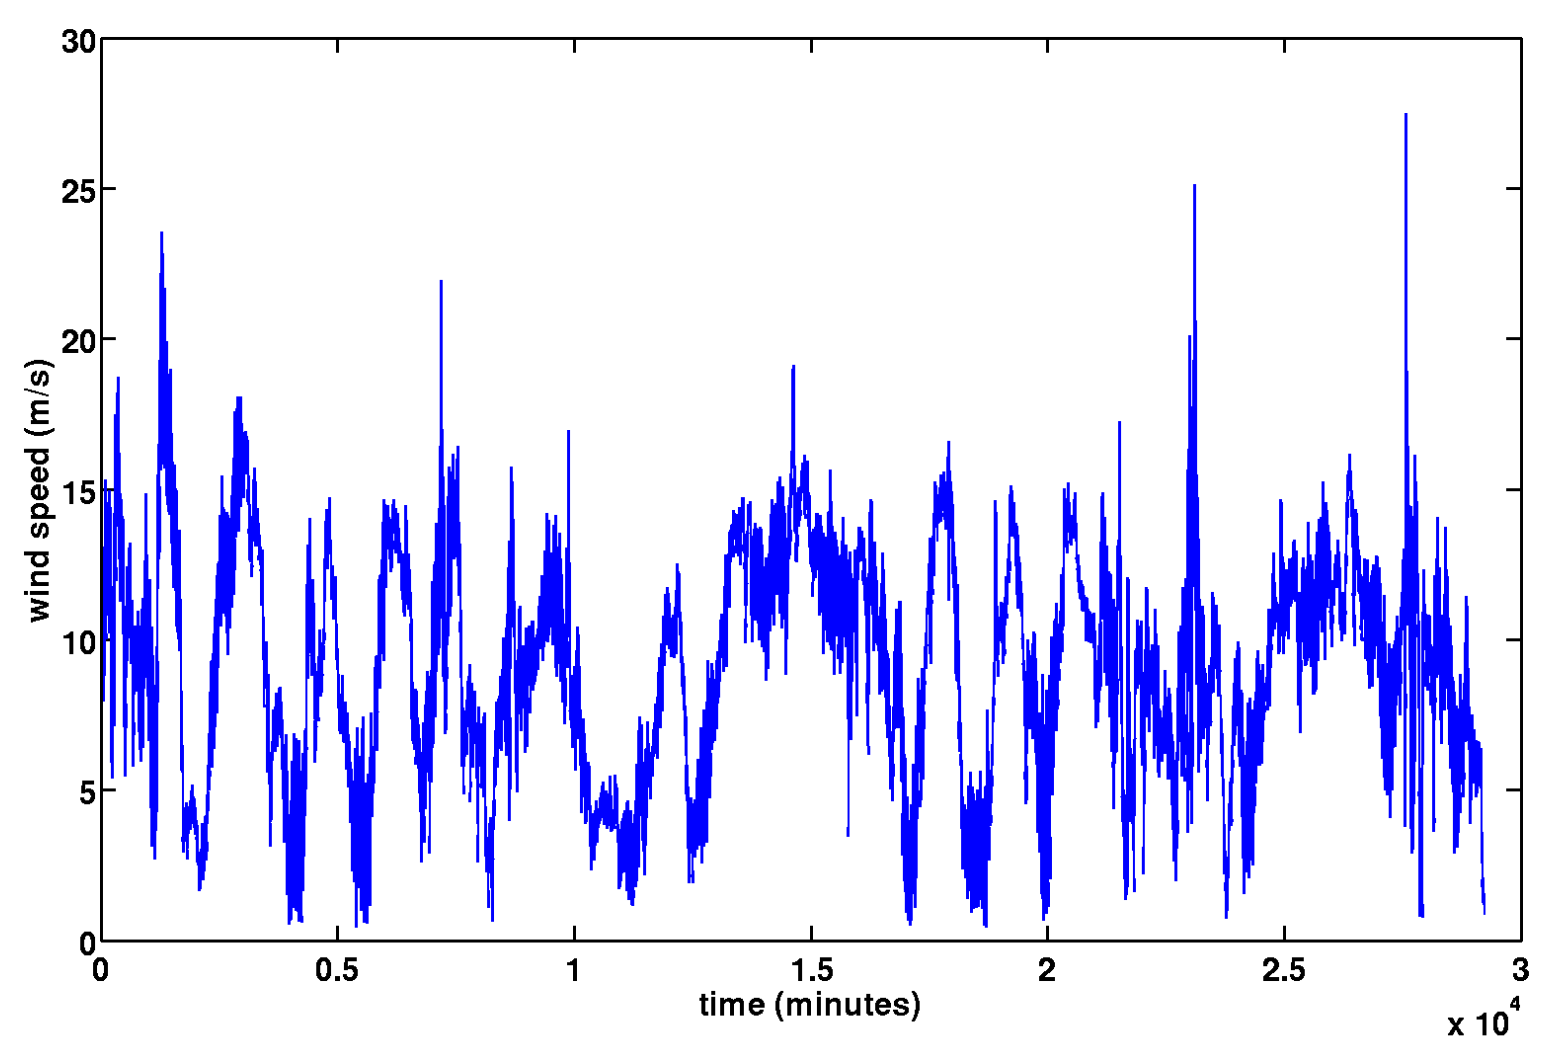
\includegraphics[width=\linewidth]{wind_mean.png}
                \caption{}
                \label{fig:figure_mean}
        \end{subfigure}%
        \centering
        \begin{subfigure}[h]{0.5\textwidth}
                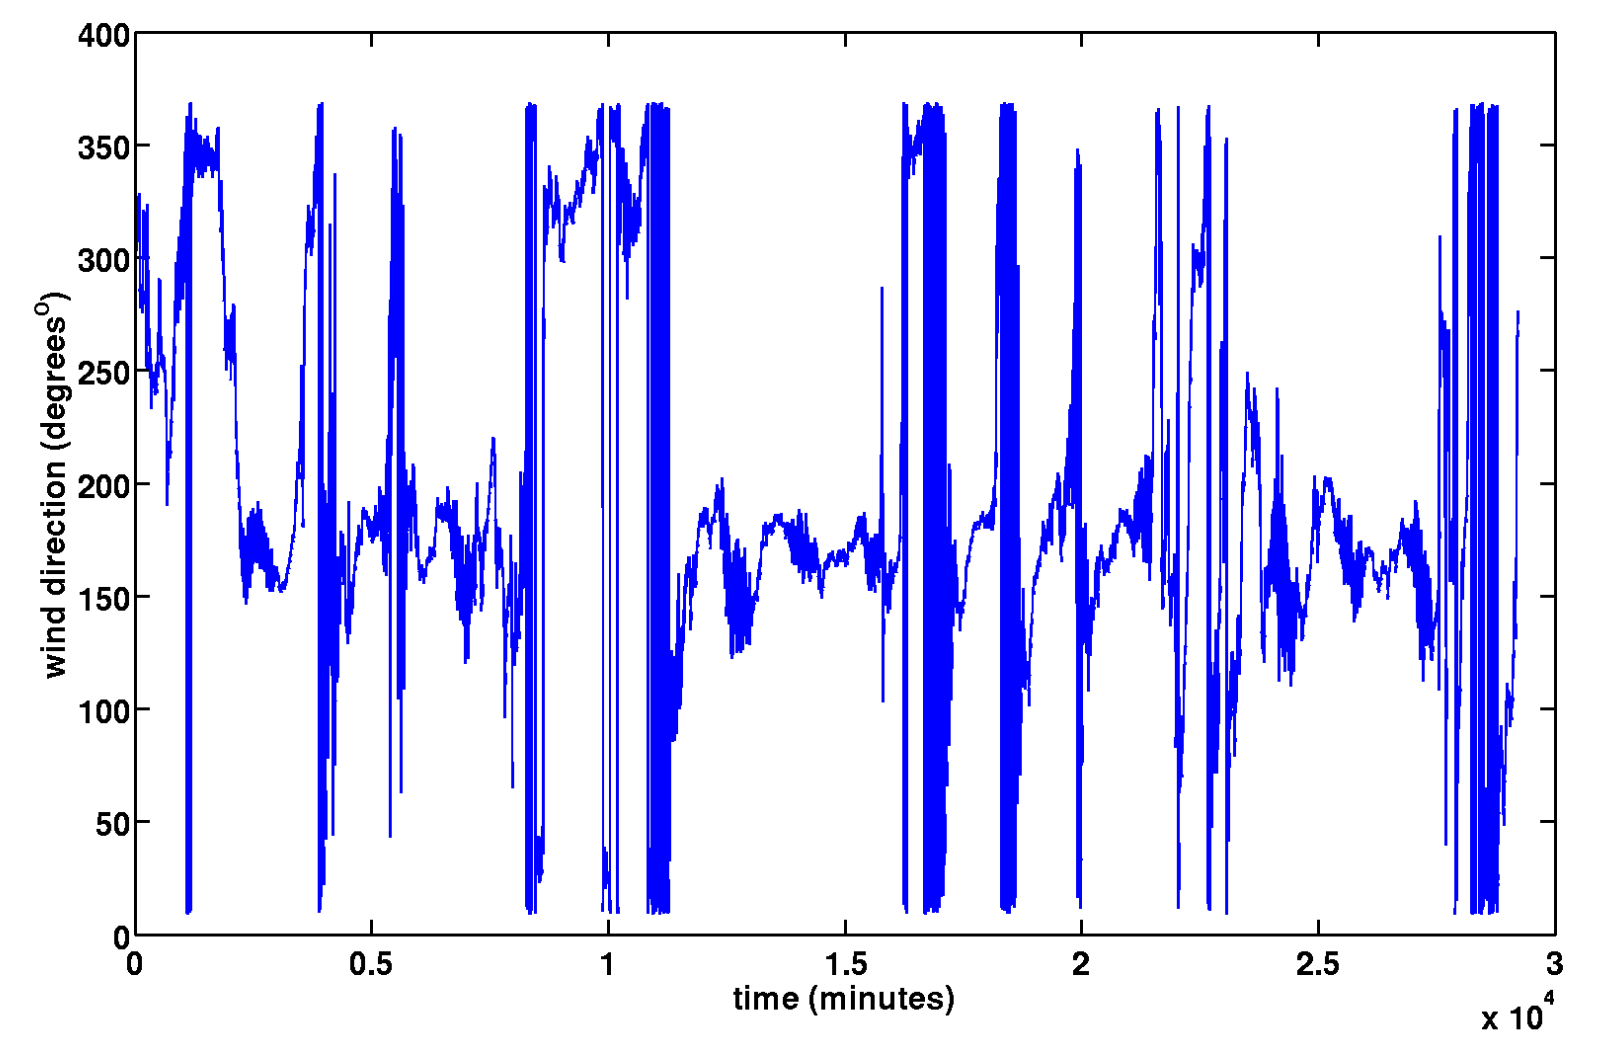
\includegraphics[width=\linewidth]{wind_direction.png}
                \caption{}
                \label{fig:dir}
        \end{subfigure}
       \caption[Wind speed and direction]{(A) Wind speed magnitude vs time    (B) Wind direction vs time, at a height of 50 m from the ground}\label{fig:windir}
\label{fig:smag}
\end{figure}
 
\begin{figure}[h!]
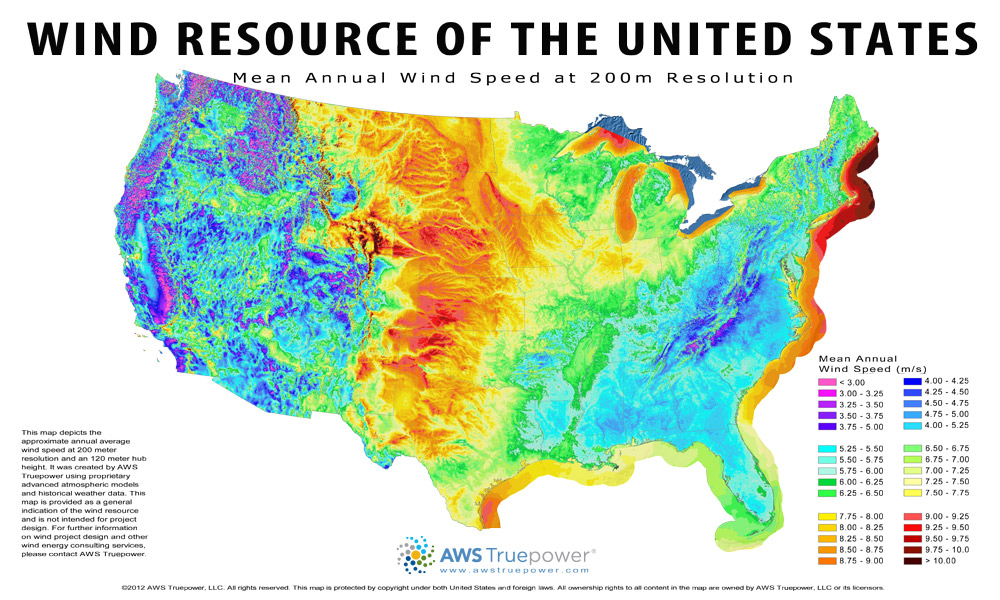
\includegraphics[width = 1.0\linewidth]{wind_us.jpg}
\caption[Mean annual Wind Speed]{Mean annual Wind Speed in different states of US. Courtesy: AWS Truepower}
\centering
\small source by:\url{https://www.awstruepower.com/} \label{fig:resource}
\end{figure}

\begin{figure}[h!]
\centering
        \begin{subfigure}[h]{0.5175\textwidth}
                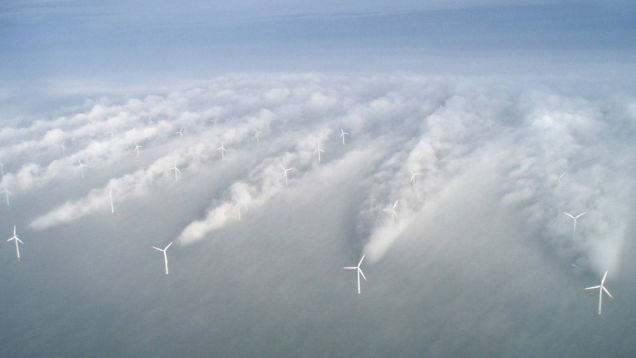
\includegraphics[width=\linewidth]{horns_rev.jpg}
                \caption{}
                \label{fig:figure_horns}
        \end{subfigure}%
        \centering
        \begin{subfigure}[h]{0.48675\textwidth}
                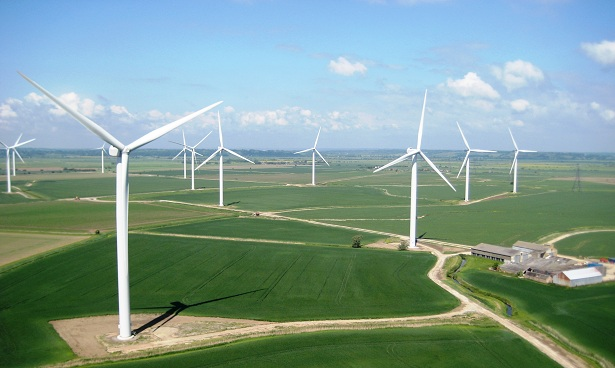
\includegraphics[width=\linewidth]{wind_onshore.jpg}
                \caption{}
                \label{fig:onshore}
        \end{subfigure}
       \caption[Offshore and Onshore wind farms]{(A) Offshore wind farm at Horn-Rev depicting wind turbine wakes (B) A classical Onshore wind farm}
\label{fig:smag}
\end{figure}

\begin{figure}[t!]
       \centering
        \begin{subfigure}[h]{0.5\textwidth}
                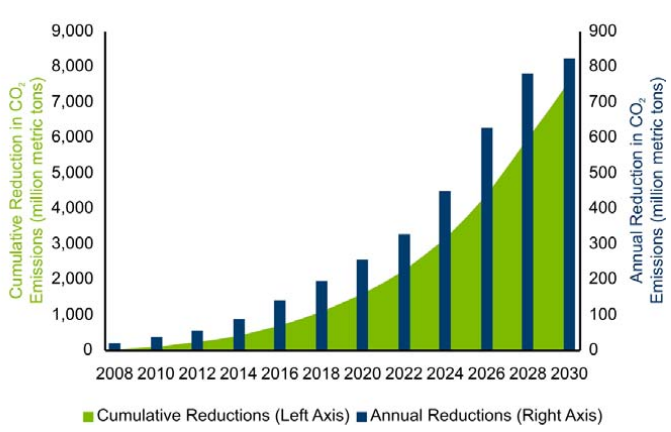
\includegraphics[width=\linewidth]{doe3.png}
                \caption{}
                \label{fig:do3}
        \end{subfigure}%
       \begin{subfigure}[h]{0.6\textwidth}
                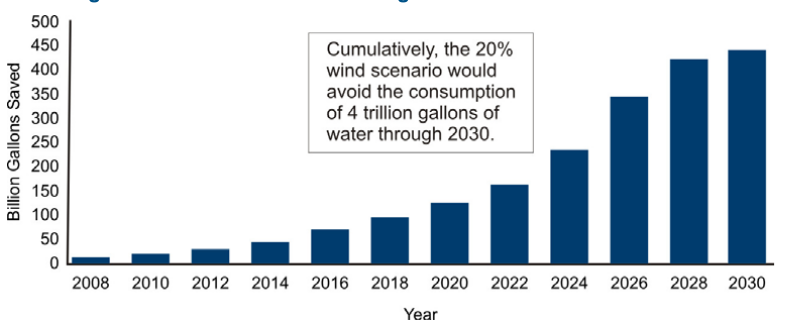
\includegraphics[width=\linewidth]{doe4.png}
                \caption{}
                \label{fig:do3}
        \end{subfigure}%
       \caption[$CO_2 \ \&$ Water Reduction]{ Propose reduction of (A) $CO_2$ emission (B) Water capacity, projected till 2030 with the goal towards ``20 \% Wind Scenario"}
\label{fig:smag}
\end{figure}


% Chapter 1

\chapter{Numerical Method} % Main chapter title

\label{Chapter2} % For referencing the chapter elsewhere, use \ref{Chapter1} 

\lhead{Chapter 2. \emph{Numerical Method}} % This is for the header on each page - perhaps a shortened title

%----------------------------------------------------------------------------------------

\section{Navier Stokes Equation}
3D Navier-Stokes equation solving for velocity field $\pmb{u}(\pmb{x},t)$, scalar pressure field ${p(\pmb{x},t)}$ with input volume force function $\pmb{f}(\pmb{x},t)$ (momentum and continuity equations).
   
  \begin{eqnarray}
\frac{\partial \pmb{u}}{\partial t} + \pmb{u}.\nabla \pmb{u} & = & -\frac{1}{\rho}\nabla p + \nu \nabla^2 \pmb{u} + \pmb{f}  \ \ \ \ \ \   \mbox{in} \ \ \ {{\Omega}} \times (0,T), \nonumber \\
\nabla.{\pmb{u}} & = & 0 \ \ \ \ \mbox{in}\ \ \ {{\Omega}} \times (0,T), \nonumber \\
\pmb{u}(\pmb{x},0) &=& \pmb{u}^{0}(\pmb{x})\ \ \ \ \mbox{for}\ \ \ \pmb{x}\in\Omega, \nonumber \\
\mathcal{B}(\pmb{u}_{b}) & = & 0 \  \  \   \  \  \   \  \  \  \  \ \ \mbox{in} \ \ \ \partial {{\Omega}}. \label{NS}
\end{eqnarray} 

Here, ${\Omega} \subset \mathbb{R}^{3}$ is the three-dimensional domain in Equation~(\ref{NS}), $\pmb{
u}^{0}(\pmb{x})$ represents the initial condition of the PDE and $\partial{\Omega}$ represents the external surface of ${\Omega}$ on which the boundary conditions $\pmb{u}_b$ are defined. \\
In the computational domain, the 3D incompressible Navier-Stokes equations along with boundary conditions are solved in weak formulation using exponentially accurate higher order spectral element methods~\cite{patera3},~\cite{patera2},~\cite{fischer_jcp} (Refer to Appendix~\ref{galproj} for details). 
  

 In spectral element methods, the weak formulation of the equations is carried out by weighted residual technique (orthogonal projection of the residual of the equations), or more specifically by Galerkin projection method~\cite{fischer_jcp},~\cite{deville} cast using the concept of inner products in functional spaces.
 
Usually, in weighted residual technique the discrete inner products are carried out using summation on the quadrature nodes defined as the roots of the orthogonal polynomials from the solutions of the Sturm-Liouville problem~\cite{sturm2}, with the corresponding quadrature weights.

It must be mentioned, that a consistent approach of using spectral element discretization involves using polynomial orders of pressure interpolants (basis functions) usually two orders lower than the velocity interpolants. This is done to essentially remove the spurious modes of pressure along the lines of finite volume approach~\cite{patera2,deville}. Using orthogonal interpolating polynomials (Legendre polynomials) as basis functions on $N+1$ quadrature nodes as defined above ensures that the numerical integration is exact for polynomials of degree up to $2N+1$. (For details of quadrature nodes, qudrature weights see Appendix~\ref{lagintp}, for Legendre polynomial see Appendix~\ref{legpol},~\ref{lagintp})

In spectral element methods~\cite{patera3},~\cite{deville},~\cite{fischer_jcp}, the decomposition of the computational domain consists of  subdividing $\bar{\Omega} = \Omega\cup \partial\, \Omega$ into $E$ non-overlapping adjacent rectilinear elements such that $\bar{\Omega} = \cup_{e=1}^{E}\Omega_{e}$. Each ${\Omega_{e}}$ is the image of a reference subdomain under a mapping\ ${\pmb{x}}^{e}(\pmb{r}) \in {\Omega_{e}} \rightarrow \pmb{r}\in {\hat{\Omega}}$, with a well defined inverse  ${\pmb{r}}^{e}(\pmb{x}) \in \hat{{\Omega}} \rightarrow \pmb{x}\in {\Omega_{e}}$, where the 3D reference subdomain is ${\hat{\Omega}} = [-1,1]^{3}$. Scalar functions within each local element ${{\Omega}_{e}}$ are represented as $N^{th}$ order tensor product polynomials on a reference subdomain ${\hat{\Omega}}$. With such decomposition, a convenient choice of the functional spaces of velocity and pressure fields as discussed before, are commonly known as $\mathbb{P}_{N}-\mathbb{P}_{N-2}$ formulation (Refer to Equations(~\ref{sob2},~\ref{sob3}) in Appendix ~\ref{galproj}).
In 3D, velocity function in the spectral element method in the element can be expressed as follows
\begin{equation}
u(r_1,r_2,r_3)|_{\hat{\Omega}} = \displaystyle\sum_{i=0}^{N_x}\sum_{j=0}^{N_y}\sum_{k=0}^{N_z}u_{ijk}^{e}\pi_{N_x,i}({r_1})\pi_{N_y,j}({r_2})\pi_{N_z,k}({r_3}),  \ \ \ {r_1},{r_2},{r_3}\in [-1,1]^3,
\end{equation}
where, $\pi_{N_x,i}(r_1),\hspace{0.5em} \pi_{N_y,j}(r_2), \hspace{0.5em}\pi_{N_z,k}(r_3)$ are the Lagrange polynomial based interpolant of degree $N_x$, $N_y$ and $N_z$.
Identically the pressure function in SEM in the local element, with $\pi^{p}_{N,j}({\zeta}) \in \mathbb{P}_{N-2}(\zeta)$ can be given as 
\begin{equation}
p(r_1,r_2,r_3)|_{\hat{\Omega}} = \displaystyle\sum_{i=1}^{N_x-1}\sum_{j=1}^{N_y-1}\sum_{k=1}^{N_z-1}p_{ijk}^{e}\pi^{p}_{N_x,i}({r_1})\pi^{p}_{N_y,j}({r_2})\pi^{p}_{N_z,k}({r_3}),  \ \ \ {r_1},{r_2},{r_3}\in [-1,1]^3
\end{equation}
 (See Equations(\ref{legendre1},~\ref{legendre2}) in Appendix~\ref{lagintp} for details abount Lagrange interpolants).\\
It must be understood that due to the invertible mapping between $\Omega_{e}$ and $\hat{\Omega}$ there exists a one-to-one correspondence between the nodal values of $u(x,y,z)|_{\Omega_{e}}$, $p(x,y,z)|_{\Omega_{e}}$ and reference subdomain values $u(r_1,r_2,r_3)|_{\hat{\Omega}}$, $p(r_1,r_2,r_3)|_{\hat{\Omega}}$ and the coefficients $u_{ijk}^{e}$, $p_{ijk}^{e}$ are the local nodal values of $u|_{\Omega_{e}}$, $p|_{\Omega_{e}}$ respectively in the nodal-based formulation. The local to global mapping of data is carried out using a boolean connectivity matrix that preserves inter element continuity.\\
\par
The differential operators in the current SEM formulation
%especially the poisson solvers in Nek5000
have been carried out using efficient implementation of tensor products(Refer to ~\cite{lynch},~\cite{orz},\cite{deville} and for details).
The block matrices formed by Kronecker/tensor products (Appendix~\ref{tens}) are advantageous since various important matrix operations required in SEM like matrix inversion, affine transformation for differentiation, eigenvalue calculations can be obtained by using these linear algebra operators on much smaller matrices than the global matrices~\cite{lynch},~\cite{deville}. Hence, tensor products are computationally very efficient in terms of parallel scalability when used in fast 2D/ 3D Poisson solvers, filtering and other linear operators in the current SEM methodology~\cite{erik}.\\

The time discretization of Navier-Stokes solver in the current spectral element code Nek5000~\cite{nek5000} involves $k^{th}$ order backward difference/extrapolation scheme (BDF/EXT) where $k = 2$ or $3$ (See ~\ref{bdf} for details.). The code is fully dealiased using $3/2$ rule~\cite{orz2,canuto}, the velocity  is solved using preconditioned conjugate gradient (CG) method and the pressure solver uses iterative generalized mean residual solver (GMRES) method in Krylov subspace.

\section{Large Eddy Simulation}\label{les}
For the mathematical formalism of LES we use the tensorial notation of the Navier-Stokes equation. In 3D, the tensorial notation of NS equation can be given by
\begin{equation}
\frac{\partial {u}_i}{\partial t} + {u}_j\frac{\partial {u}_i}{\partial x_j} = -\frac{1}{\rho}\frac{\partial {p}}{\partial x_i}  + {F_{i}} + \nu\frac{\partial^2{u}_i}{\partial x_j \partial x_j} \label{nseq}
\end{equation}
For very large $Re$ there is a large separation between the largest integral scales and smallest dissipative (Kolomogorov) scales of motion. The large eddy simulation thus aims at capturing the spatio-temporal evolution of large scales of motion while modelling the relatively smaller scales also known as the subgrid scales of motion. \\
The dynamical equation of the largest scales of motion can be obtained by applying a low-pass filtering to the Navier-Stokes equation.\\
For any scalar field $\phi(\pmb{x},t)$ the filtering in physical space can be represented as a convolution product. The resolved part $\widetilde{\phi}(\pmb{x},t)$ can be written as
\begin{equation}
\widetilde{\phi}(\pmb{x},t) = \iint_{\Omega}
\phi(\pmb{\xi},t')G(\pmb{x}-\pmb{\xi},t-t')\mathrm{d}t'\mathrm{d}^3\xi
\end{equation}
with the convolution kernel $G$ being the characteristic of the filter used and $\Delta$ and $\tau_c$ are cutoff scales in space and time associated with the kernel. Even though the filtering performed in large eddy simulation is mostly spatial in nature,  it imposes and inherent temporal cut-off scale as well~\cite{sag}.\\
The filtered NS equations can be given as
\begin{equation}
 \begin{split}
 \frac{\partial \widetilde{u}_i}{\partial t} + \widetilde{{u}_j\frac{\partial {u}_i}{\partial x_j}} + \frac{1}{\rho}\frac{\partial \widetilde{p^{*}}}{\partial x_i}  -\widetilde{F}_{i}  - \nu\frac{\partial^2\widetilde{u}_i}{\partial x_j \partial x_j}  = - \frac{\partial \tau^{\small SGS}_{ij}}{\partial x_j} \\ 
 -\boxed{\int_{\partial \Omega} G( \pmb{x} - \pmb{\xi} )[p(\pmb{\xi}) - \nu\left(\frac{\partial {u}_i}{\partial x_j}\left(\pmb{\xi}\right) + \frac{\partial {u}_j}{\partial x_i}\left(\pmb{\xi}\right) \right)]n_j \mathrm{d}S} \label{eqbc1}
 \end{split}
 \end{equation} 
 \begin{equation}
 \begin{split}
  \frac{\partial \widetilde{u}_i}{\partial x_j} = - \boxed{\int_{\partial \Omega} G\left(\pmb{x} -  \pmb{\xi}\right)u_jn_j(\pmb{\xi})\mathrm{d}S} \mapsto 0 \label{eqbc2}
 \end{split}
 \end{equation} 

where the ``tilde" represents the low-pass filtered variable and $\widetilde{u}_i$ is the instantaneous filtered velocity field in the $i^{th}$ direction. The boxed terms in Equations(~\ref{eqbc1},~\ref{eqbc2}) are direct consequence of \textit{integration by parts} $\&$ \textit{Gauss Divergence Theorem} and can be attributed as boundary commutation errors (Adressed in Section~\ref{nwm}, for detailed derivation, see ~\cite{bers}) In this respect, we would like to point out that $x$ is the streamwise direction, $y$ is the spanwise direction and $z$ is the wall-normal direction of flow.\\

Usually the filter chosen in the practise of LES is a linear operator and satisfies some fundamental properties like conservation of constants, principle of linear superposition and commutation with other linear operators like differentiation. Consequently, the non-linear convective term is the only term in the NS equation that gives rise to commutation error in the interior of the flow domain $\Omega$ (The boundary commutation errors are neglected for the time-being).
\begin{equation}
\frac{\partial \widetilde{u}_i}{\partial t} + \widetilde{u}_j\frac{\partial \widetilde{u}_i}{\partial x_j} = -\frac{1}{\rho}\frac{\partial \widetilde{p^{*}}}{\partial x_i} + \frac{\partial \tau^{\small SGS}_{ij}}{\partial x_j} + \widetilde{F_{i}} + \nu\frac{\partial^2\widetilde{u}_i}{\partial x_j \partial x_j} \label{leseq2}
\end{equation}
The modification to the original Navier-Stokes equations thus comes with an additional subgrid stress tensor $\tau^{\tiny SGS}_{ij}(u_i,u_j)$ which arises due to the filtering of the non-linear term , which is given by
\begin{equation}
\tau^{\tiny SGS}_{ij} =  \widetilde{u}_i\widetilde{u}_j - \widetilde{{u}_i{u}_j}.
\end{equation}
The modified pressure in the filtered equation can be given as
\begin{equation}
\widetilde{p^{*}} = \widetilde{p} + \frac{1}{2}\rho\widetilde{u_i}^2
\end{equation}
The interior closure problem of LES thus relies on developing a realistic model of $\tau^{\tiny SGS}_{ij}(u_i,u_j)$ by using a function $S_{\tau}(\widetilde{u}_i,\widetilde{u}_j)$. It is quite straightforward to visualize that the transfer of subgrid energy from the large to small scales of motion can be given as $-\tau^{\tiny SGS}_{ij}(u_i,u_j)S_{ij}$ which manifests that the effects on smaller scales of motion rely on the subgrid stress model.\\

Some of the fundamental properties of $\tau^{\tiny SGS}_{ij}(u_i,u_j)$ that potentially needs to be seen in the closure $S_{\tau}(\widetilde{u}_i,\widetilde{u}_j)$ are enumerated below.
\begin{itemize}
\item $\tau^{\tiny SGS}_{ij}$ is translation and rotation invariant
\item $\tau^{\tiny SGS}_{ij}$ is symmetric and reflective: $\tau_{ij} = \tau_{ji}$; $\tau_{ij}(-u_i,-u_j) = \tau_{ij}(u_i,u_j) $
\item $\tau^{\tiny SGS}_{ij}$is realizable: $\tau^{\tiny SGS}_{ij}(u_i,u_j)\xi_i\xi_j \geq 0, \ \ \forall \xi \in \mathbb{R}^{3}$ 
\item Finite turbulent kinetic energy and $\vert\vert \tau^{\tiny SGS}_{ij}(u_i,u_j) - S_{\tau}(\widetilde{u}_i,\widetilde{u}_j)   \vert\vert \ \leq C(u_i)\Delta^{\alpha}$ for some $\alpha \geq 0$
\item $\tau^{\tiny SGS}_{ij}$ is essentially dispersive and \textbf{not dissipative} in nature
\end{itemize}

Large eddy simulation has a rich history of development of the subgrid stress model and they can be broadly classified as \textit{physics based / functional models} and \textit{mathematical models} which can be further subclassified as \textit{regularization models} $\&$ \textit{structural models}. The physics-based models are mostly dissipative in nature (eddy viscosity models)~\cite{smagorinsky,deardoff,schumann,grot,mason,germano,lily,katz,porte1fun,bou1}. The eddy-viscosity models developed from the stability issues associated with the dynamics of the filtered NS equations at high $Re$, yet providing a meaningful description of the bulk energy transfer from the larger to the smaller subgrid scales (no backscatter of energy) with a poor representation of the eigenvectors of stress tensor. On the other hand, the mathematical model evolved separately as regularization models seeking uniqueness of 3D weak solutions~\cite{lad,lad2,holm,karmanos,guermond,guerts} or the structural models e.g., rational LES ~\cite{il1,il2}, deconvolution models extracting the information of the small scales (energy spectrum) lost by low-pass filtering~\cite{bardina2,bal3,stolz,lay2,dunca,sag,bers}. The structural model thus consists in making the best approximation of the tensor $\tau_{ij}$ by constructing it from an evaluation of $u$ or a formal series expansion . The modeling assumption therefore consists in using a relation of the form $\tau = H(\widetilde{u})$ which provides accurate representation of stress eigenvectors, despite a relatively poor depiction of the subgrid energy transfer (depicts backscatter of energy). However the deconvolution models like the scale-similar models~\cite{bardina2,lay2} or the relatively new Stolz-Adams model~\cite{stolz,dunca} which model dispersive functions of the subgrid stress $\tau_{ij}$ may be unstable if used only in itself. Hence to bridge the gap between the eddy viscosity and structural models, most of the deconvolution models have been used in conjunction  with an additional dissipation not only to impart stability to the system but also combining the strength of the functional and structural models~\cite{bardina,zhang}.\\
\par
In the studies of large $Re$ atmospheric boundary layer flows used in the current dissertation, we use eddy-viscosity type dissipative models or more specifically Smagorinsky model which has a profuse history in the ABL LES community~\cite{mason,sull,katz,porte1fun,bou1,brass,meyers2}. The assumption in this model is that the deviatoric part of the subgrid scale stress tensor can be modelled using analogous methodology of Boussinesq's hypothesis (gradient diffusion hypothesis) in the filtered velocity field,
\begin{equation}
\tau^{SGS}_{ij} - \frac{1}{3}\tau^{SGS}_{kk}\delta_{ij} = 2(C_s\Delta)^2|\widetilde{S}|\widetilde{S}_{ij}, \label{sgs}
\end{equation}
where $\widetilde{S}_{ij} = \frac{1}{2}({\partial \widetilde{u}_i}/{\partial x_j}+ {\partial \widetilde{u}_j}/{\partial x_i})$ is the filtered strain rate and the magnitude of the strain tensor $|\widetilde{S}| = \sqrt{2\widetilde{S}_{ij}\widetilde{S}_{ij}}$. In classical Smagorinsky model~\cite{smagorinsky}, filter length scale $l_f$ is assumed to be proportional to the grid filter width $\Delta$, and $C_s$ is the non dimensional Smagorinsky coefficient. The grid filter width $\Delta$ is calculated as $(\Delta x\Delta y\Delta z)^{1/3}$, where $\Delta x, \Delta y, \Delta z$ are the central difference between GLL nodes at the interior and one sided difference at the boundaries.\\

The methodology by which $C_s$ in dissipative models is calculated are mainly of two types \textit{static} and \textit{dynamic}. In static methods usually $C_s$ (a constant value) is directly implemented in the code. Lily (1967)~\cite{lily0} predicted Smagorinsky coefficient $C_s \sim 0.16$ for isotropic turbulence from the equilibrium of subgrid dissipation ($-\tau_{ij}\widetilde{S}_{ij}$) and viscous dissipation ($\varepsilon = 2\nu \int_{0}^{\infty}k^2E(k)dk$). However, wall-bounded or mean sheared flows, have shown a sensitive dependance of $C_s$ on the magnitude of shear, and a $C_s \sim 0.16$  was overly dissipative in the near wall region, damping large-scale fluctuations and restricting the near wall coherent eddies to develop that aid in turbulent transport~\cite{hor,bers}. Consequently, such high values of Smagorinsky coefficient predicted unrealistic slopes of the mean velocity profile (mean shear), which is commonly known as the ``log-layer mismatch" especially in high $Re$ ABL flow community (deviation of the mean velocity profile from the logarithmic trends)~\cite{andren,meyers2}. In Channel flow simulations various $C_s$ has been reported in the literature, e.g. $C_s \approx 0.1$~\cite{deardoff}, $C_s \approx 0.09$~\cite{bardina2}, while~\cite{moin1} reported $C_s \approx 0.065$ for acceptable results (In fact ~\cite{moin1} reported the filter-scale metric $\Delta$ to be twice as ~\cite{deardoff,bardina}, so essentially, with same $\Delta$ to all of them $C_s$ reported by ~\cite{moin1} would be indeed $\approx \ 0.13$). However, simple reduction of $C_s$ is not good enough, since near wall physics also requires that the mixing lengths and hence $C_s$ are damped near the wall such that it can capture the essential dynamics of near wall eddies.\\
 In wall-bounded flows like channel flows, flat plate boundary layer etc., a wall damping function is usually added near wall to circumvent the overly-dissipative effects of a constant $C_s$ value. These are usually done by Van-Driest damping factor~\cite{van-Driest} of the form
\begin{equation}
l_f^2 = (C_s\Delta)^2\left(1 - \exp(\frac{z^{+}}{A^{+}})\right)^2
\end{equation}
with $A^{+} = 26$ and plus units denote normalization by $\delta_v = \nu/u_{\tau}$.\\
The dynamic version was first brought to the LES community with classic paper of Germano et. al~\cite{germano} and its modification by Lily~\cite{lily} where $C_s$ is dynamically calculated at each timestep assuming scale-invariance of $C_s$ at LES filter with cutoff scale $\Delta$ and a test filter with a cutoff scale of $2\Delta$. This model eliminated the need to bruteforce the value of $C_s$ to the numerical model, tailor-made for different turbulence problems. Further advanced models like dynamic models with lagrangian averaging~\cite{mene1} where averaging of coefficients in the dynamic modelling are done through lagrangian particle tracking, assuming power law dependance of $C_s$ e.g. scale-dependant dynamic Smagorinsky model ~\cite{porte1fun,bou1} has also been proposed which hold for large $Re$ ABL flows. The supposed advantage of dynamic models is improved accuracy compared to its standard counterpart, and the near wall damping of mixing length of wall bounded flows are automatically ensured. The obvious disadvantage is the additional computational costs to calculate $C_s$ at each time step and stability issues which creates stringent time-steps in dynamic models compared to the standard bruteforce models.\\
\par
In the present study, for high Reynolds number turbulent ABL flow, we use standard Smagorinsky model with algebraic wall damping by Mason and Thompson (1992)~\cite{mason}.
\begin{equation}
\frac{1}{l_f^{n}} = \frac{1}{(C_s\Delta)^{n}} = \frac{1}{(C_s\Delta)^{n}} + \frac{1}{\kappa(z + z_0)^{n}} \label{mas}
\end{equation} 
Equation~(\ref{mas}) essentially uses an ad-hoc blending function with parameters $C_0, n$, such that the filter length scale gradually decreases as we approach the wall. Also in the context of atmospheric boundary layer simulations,~\cite{mason_callen,mason}, $l_f$ can also be interpreted as the mixing length of the subgrid scale eddies. Here $\kappa$ is the Von-Karman constant and $z_0 \ll H$ is the aerodynamic roughness length of the bottom ``wall". An asymptotic analysis of the filter length $l_f$ reveals that
\begin{equation}
\lim_{z \rightarrow \infty} l_{f} (z; z_0, C_0,n) = C_0 \Delta, \ \ \ \ \  l_{f} (z = \epsilon; z_0, C_0,n) \approx \kappa (\epsilon + z_0),\ \ \epsilon \sim O(z_0) \ll H, \label{mas2}
\end{equation}
From Equation~\ref{mas2}, it can be observed that at height $z \sim O(H)$, i.e. at the outer layer, it has conventional Smagorinsky length scales ($l_f \sim C_0 \Delta$) for SGS stress, while it retrieves scales corresponding to the log-law $l_f \ \sim \kappa (z + z_0)$ as it approaches near-wall~\cite{mason0,mason}. These scales are essentially the mixing length of ``inertial" subgrid eddies. It is important to note that even though the asymptotic scaling is independant of $n$, the numerical scaling is a strong function of $C_0, n$ (See Figure~\ref{fig:figure_smag}). For $n = 2, 3$,      $ l_f$ saturates to a value $C_0 \Delta$ at $z \lessapprox H/2$, while at $n = 1$, $l_m$ saturates to $C_0\Delta$ at $z \sim H$ and at $n = \frac{1}{2}$, it would never saturate within the ABL ($z \gg H$) and $l_f < C_0\Delta$ even at the outer layer. This algebraic damping function can be viewed analogous to the Van-Driest damping function~\cite{van-Driest,bers} for smooth wall-resolved LES. Various values of parameter{s} $C_0, n$ have been reported in the literature, e.g. Mason and Thompson~\cite{mason} used both $n = 1 \ \& \ 2$ with $C_0$ in a broad range of 0.13 to 0.32 (keeping $C_0\Delta$ at fixed different values)  Port$\acute{e}$-Agel et. al~\cite{porte1fun} used $C_0 = 0.1-0.17$, $n = 1,2$ respectively, Bou-Zeid et al.~\cite{bou1} reported $C_0 = 0.16, \ n = 2$ while Calaf et al.~\cite{calaf} published $C_0 = 0.13$ and $n = 3$ for their simulations. 
 \\
\par 
However, using these values without analysing their values on dissipation effects and hence tuning is problematic in spectral element methods, since these values are mostly used in conjunction with 2nd order central difference~\cite{porte1fun,porte1a}, or 4th order conservative finite difference~\cite{meyers2} in the wall normal direction, which are quite dissipative and dispersive as compared to the exponentially accurate SEM. Using these values directly, in SEM would result in vigorous streamwise spatial oscillation in the near-wall region for the resolved kinematic shear stress. Considering this, we always use $C_0 \sim 0.15-0.17$, with $n = 0.5, 1, 2, 3$ in our current spectral element simulations without invoking too much numerical error into the system. 
\begin{figure}
\centering
        \begin{subfigure}[t]{0.5\textwidth}
                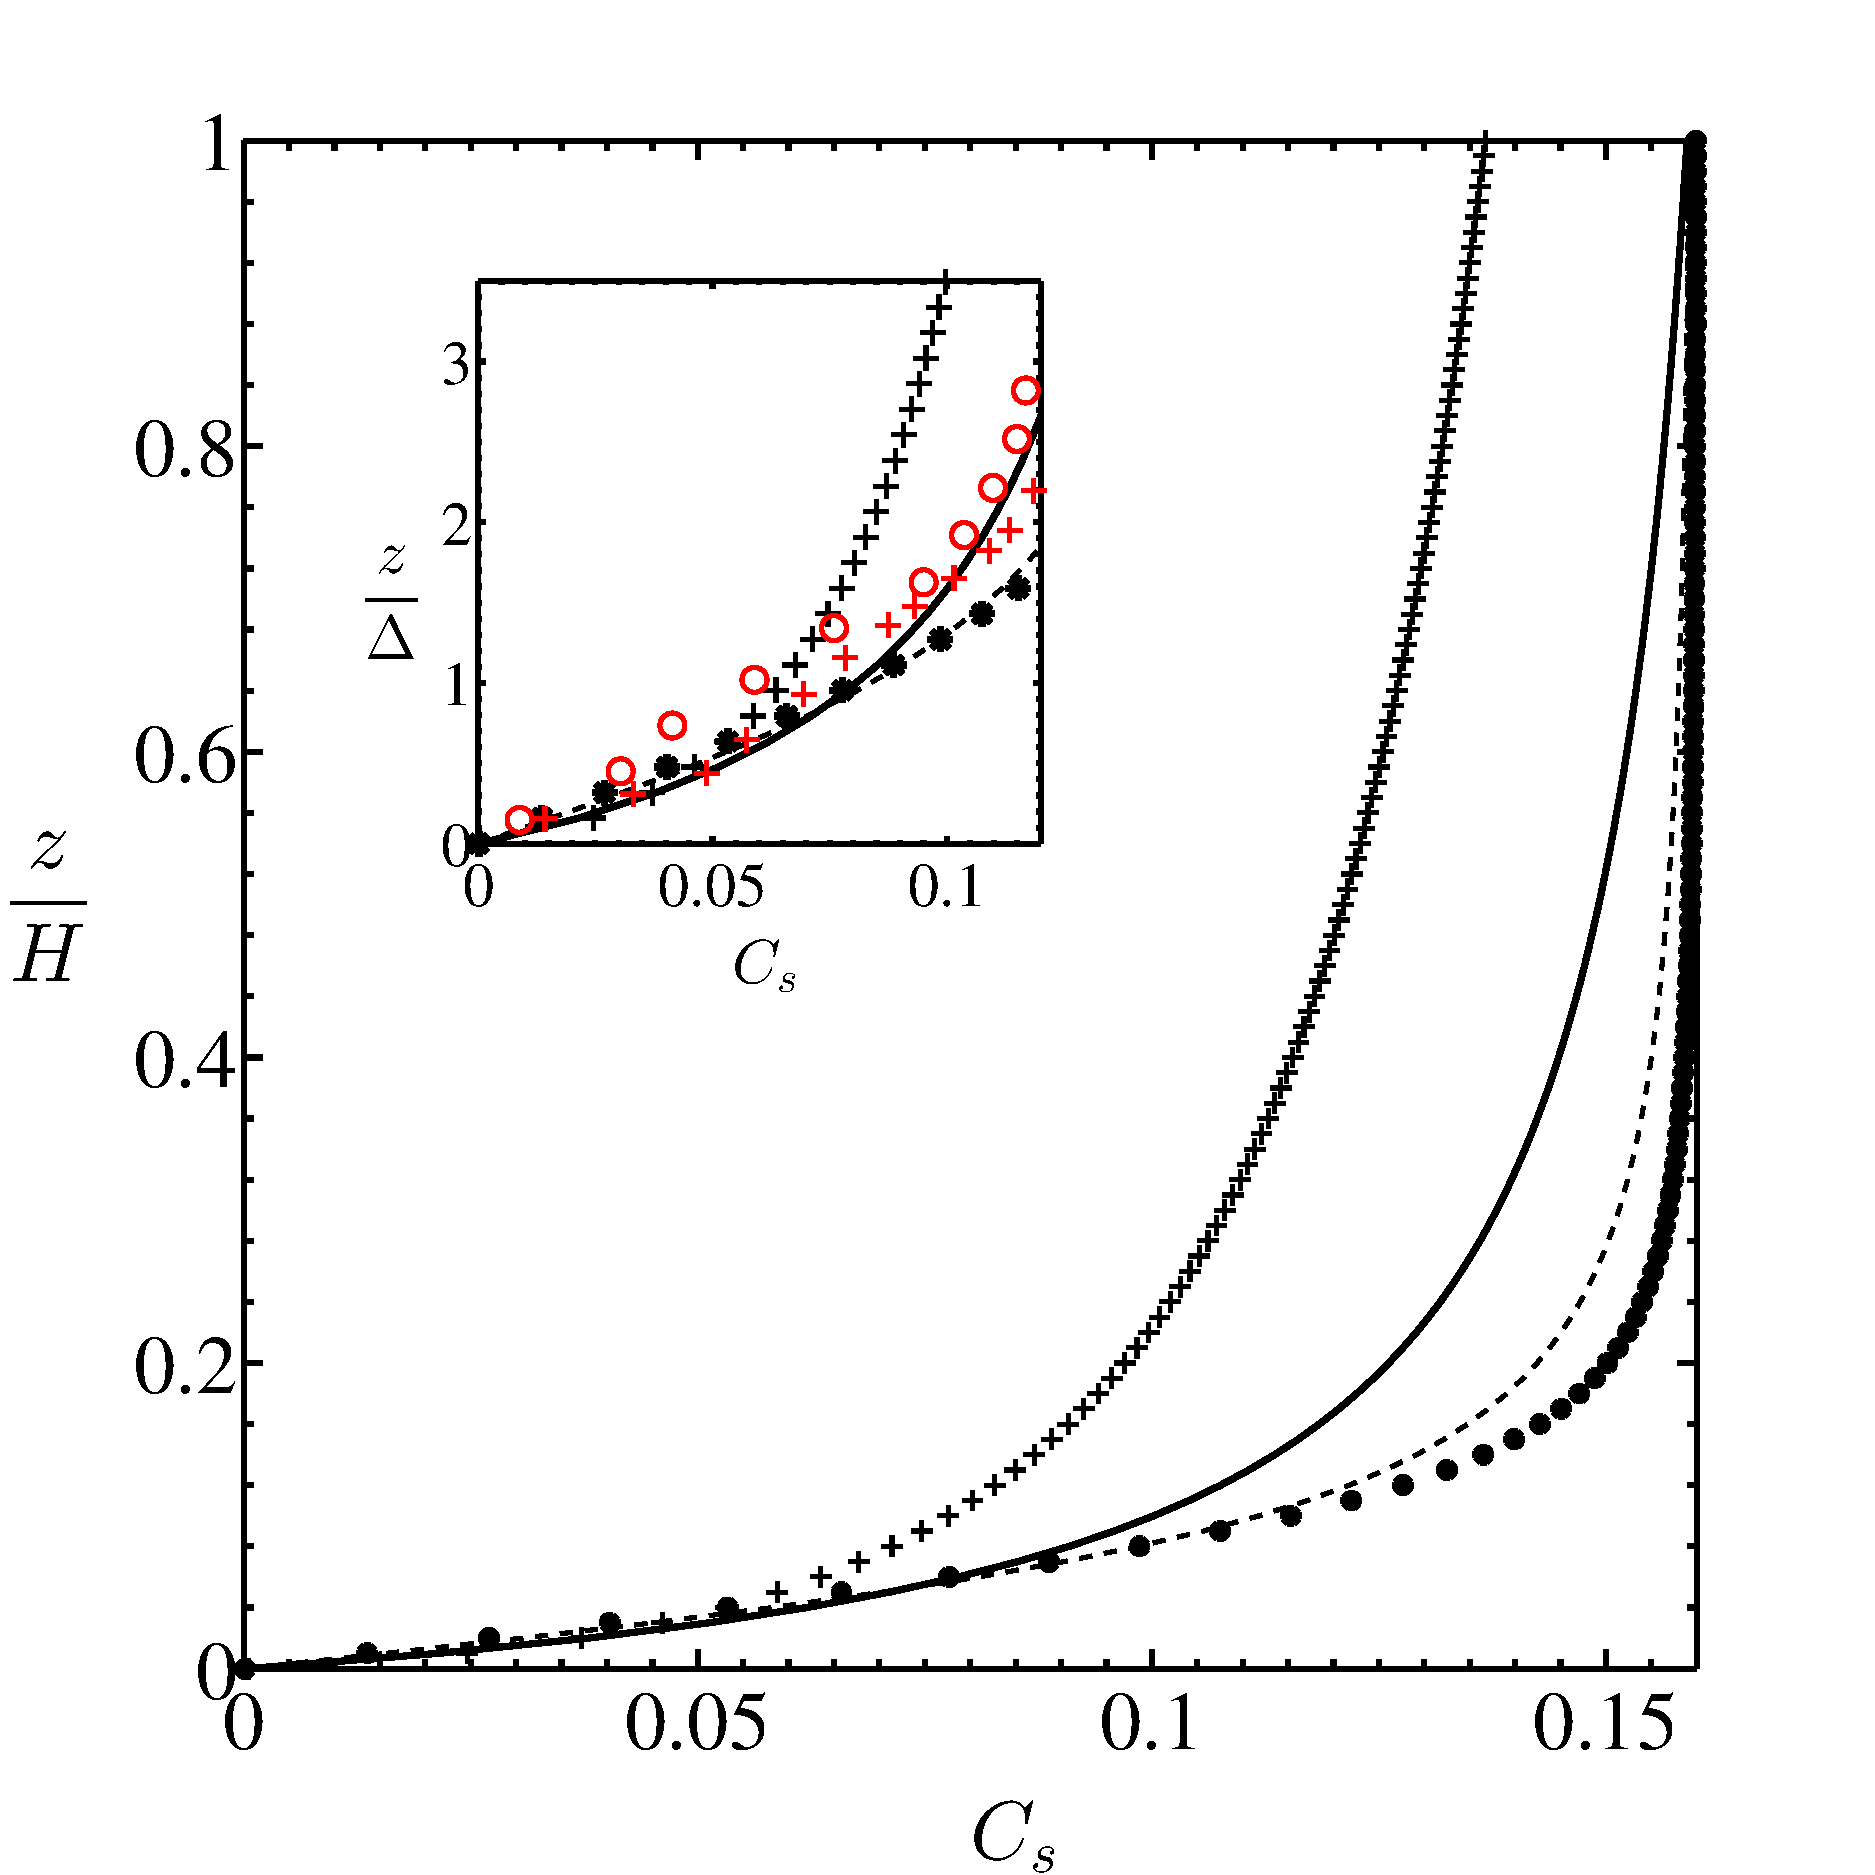
\includegraphics[width=\linewidth]{Figure/Smag2b.pdf}
                \caption{}
                \label{fig:figure_smag}
        \end{subfigure}%
        \centering
        \begin{subfigure}[t]{0.5\textwidth}
                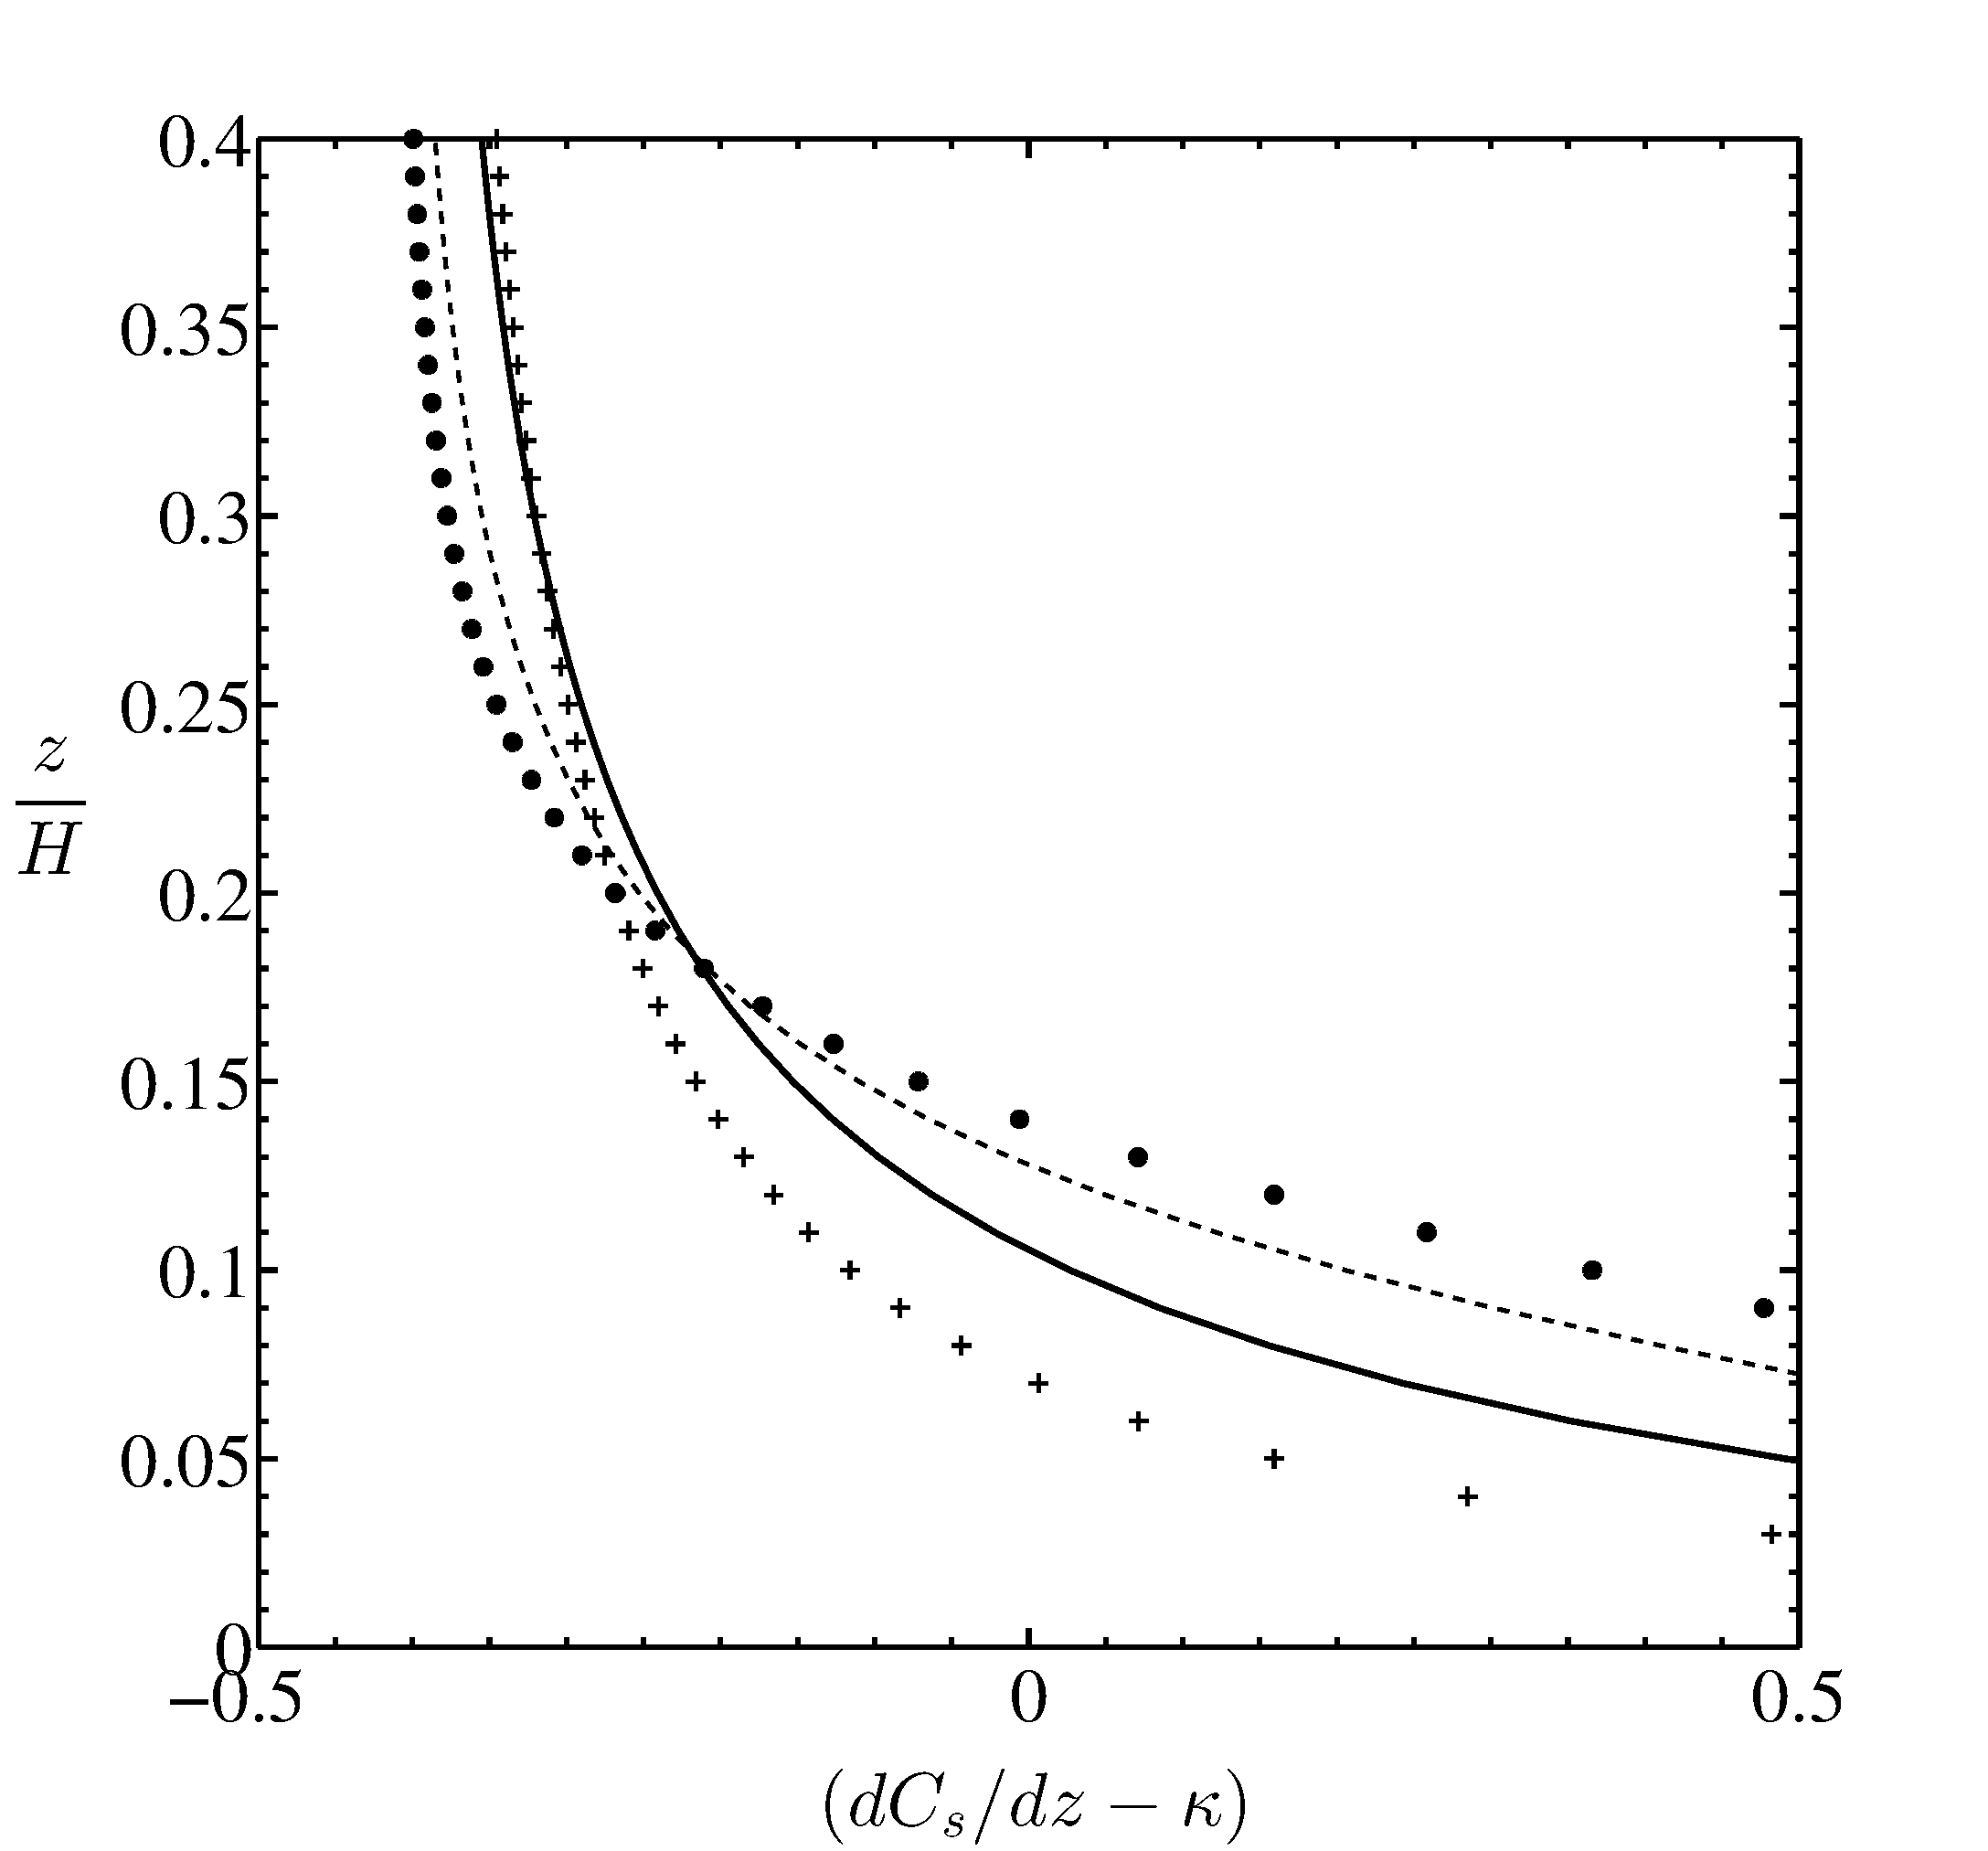
\includegraphics[width=\linewidth]{Figure/Smag2b_der.pdf}
                \caption{}
                \label{fig:smagd}
        \end{subfigure}
       \caption[Smagorinsky coefficient $C_s$ vs $z/H$ for different $(C_0, \ n)$]{(a) Smagorinsky coefficient $C_s$ vs $z/H$. Inset: variation of $C_s$ vs $z/\Delta$, zoomed-in. (b) $\frac{dC_s}{dz}-\kappa$ vs $z$.   $+$ black, $n = 0.5$; $-$ black, $n = 1$; $--$ black, $n = 2$; $\star$ black, $n = 3$; red $+$ dyn. Smagorinsky, red $o$, scale dependant dyn. Smagorinsky, Porte-Ag\'{e}l et. al (2000). $C_0 = 0.16$, fixed ($C_0 = 0.19$ for $n = 0.5$). $\kappa = 0.41$, Von Karman constant. $z_0 = 10^{-4}H$.}
\label{fig:smag}
\end{figure}

Figure~\ref{fig:figure_smag} shows the variation of Smagorinsky coefficient $C_s$ for various parameter tuples $\lbrace C_0, \ n \rbrace$ with height $z$ normalized with boundary layer thickness $H$ and also with grid scale $\Delta$. It is also observed from the  figure, that decreasing $n$ tends to smoothen the blending function in algebraic damping near wall or $\frac{dC_s}{dz}$ increases with lower value of $n$, especially in the top $10\%$ of the inner layer ($z/H \sim 0.08 - 0.10$). Additionally, with $n \downarrow$, at the upper part of ABL, the value of $C_s$ saturates to a much lower value than its classical counterpart $\sim 0.16$~\cite{lily0}.  Figure~\ref{fig:figure_smag} thus justifies the use of higher value of $C_0$ ($C_0|_{n=\frac{1}{2}} > C_0|_{n=1} > C_0|_{n=2}$), when using low value of $n$ to keep the subrid dissipation length scales ($l_f$) approximately of the same magnitudes in all the cases. It was also observed that for $n = \frac{1}{2}$, the mixing length coefficient has a reasonable comparison with the scale dependant model of Port\'{e}-Agel~\cite{porte1fun} near $z/\Delta \sim 1$.\\

In Figure~\ref{fig:smagd}, we observe that with decreasing $n$, the intersection between the curves $h(z) = (d(C_s\Delta)/dz - \kappa)$ and $g(z) = 0$ shifts downwards towards lower values of $z$ (towards log-law) within $10\%$ of the boundary layer~\cite{porte1fun,brass,meyers2} This would mean that a small region of $C_s\Delta \approx \kappa z$ can be observed within the log-layer for $n = 1/2$, which is a physically consistent phenomenon.
In this context we must mention that a relatively new methodology has already been performed to estimate the error due to SGS modelling in high Reynolds number LES done by Meyers et al.~\cite{meyers_err}. However the methodology solely concentrated on the optimization problem of the LES error metric (in wave number space) in a plane of $(C_0 \in (0.09-0.15), \ n \in(1-3))$, the two parameters in standard Smagorinsky model as suggested by Mason and Thompson~\cite{mason}. Additionally, the error metric has been compared with the log-law $\log(z/z_0)$ over the whole atmospheric boundary layer which may not be physically justifiable (see Section~\ref{nwm}). In the current study we present results with $(C_0, \ n)$ not reported previously in ABL literature~\cite{porte1fun,meyers_err,meyers2} but also elucidates a better physical understanding of the parameters $C_0, \ n$ which will be further discussed in Section~\ref{results}.
\section{Model Assumptions: Boundary conditions of ABL}\label{ablBC}
The current simulation deals with generating a feasible ABL flow field that is intercepted by the wind turbine. The simplest case is the neutral ABL simulations, where the turbulence is generated from the shear in the flow over rough wall terrain. Our present model uses $x$ as the streamwise direction, $y$ as the spanwise direction and $z$ as the wall normal direction in a cartesian framework as discussed in section~\ref{secl}. The mean streamwise velocity profile of ABL  in the surface layer (roughly $10 \sim 20\%$ of boundary layer)~\cite{basin,porte1fun,brass,meyers} can be given as
\begin{equation}
\bar{U}(z) = \frac{u_{\tau}}{\kappa}\ln \frac{z}{z_0} + \frac{u_{\tau}}{\kappa}\psi_m(\frac{z}{L_M}),\ \ \  z \gg z_0  \label{logvel}
\end{equation}
where, $u_\tau$ is the friction velocity scale, $z_0$ is the aerodynamic roughness length and $\kappa = 0.4$ is the Von Karman constant, $\psi_m$ is a non dimensional momentum stability function and $L_M$ is stability length scale by Monin and Obukhov.~\cite{obu,basin}. For neutral ABL, $L_M\rightarrow \infty$ and hence the mean velocity profile is essentially logarithmic in nature in the surface layer~\cite{obu} with $\psi_m \rightarrow 0$.\\
The boundary layer (BL) thickness for flat plate type of turbulent flows can be usually expressed as $\delta/x \sim Re_{x}^{-p}$, where $p$ is very close to 1 ($p = 0.8$ for turbulent flow over smooth flat plate)\cite{schlichting}. Consequently, the streamwise growth of the turbulent BL, could be expressed as $d\delta/dx \sim Re_{x}^{-(1+p)} $.
Since $Re_x \approx 10^8-10^{12}$ for ABL flows, the growth of the turbulent BL $d\delta/dx \approx 0$ rendering periodic boundary condition in the homogeneous streamwise direction feasible. The spanwise boundary conditions are periodic since it is consistent with the physics of the flow. The top boundary condition is a stress free lid similar to the flat plate flow, i.e., $d{\tilde{u}}_{x}/dz = d{\tilde{u}}_{y}/dz = {\tilde{u}}_{z} = 0$. For extremely high $Re$ ABL flows, the viscous sublayer $\delta_\nu/\delta \sim O(Re_{\tau}^{-1}) \approx 0$, and the aerodynamic roughness $z_0 \gg \delta_\nu$ ($\delta_{\nu} = \nu/u_{\tau}$, $\delta$ ABL thickness). Since the viscous layer cannot be resolved in such simulations, the use of shear-stress boundary conditions as near-wall modelling LES becomes imperative. Consequently, the bottom rough wall model for ABL has been developed from the log-law of the wall coupled with Monin-Obukhov similarity theory~\cite{obu} and near wall shear stress model of Schumann~\cite{schumann} and was further used by Businger et al.~\cite{basin}, Moeng ~\cite{moeng1} and Stoll and Port$\acute{e}$-Agel ~\cite{porte1a}.
\subsection{Near Wall Modelling}\label{nwm}
\par
\ \ \ We now discuss in details the complete approximate boundary conditions which we use at the bottom ``wall". For the mathematical formalism of the closure of momentum flux at bottom wall boundary condition see Appendix~\ref{stresseq}.\\
\  From now onwards, we refer to the momentum flux (shear stress) with the notation $\tau_{,s}$ for brevity. The shear stress boundary conditions for near-wall modelling are calculated from the ``in-phase" filtered resolved velocity fields half a grid node away from the ``wall" (non-local dependance)~\cite{bers} satisfying log-law (also from Monin-Obukov similarity theory)~\cite{obu} near the wall in Reynolds-average sense~\cite{pio2,jimtech,lars}. To complete the bottom wall boundary conditions we also invoke a no-penetration condition $\widetilde{w} \ = \ 0$ which is consistent with the physics of near wall large eddies~\cite{maxwell,porte1fun,bers}.
\begin{equation}
\frac{\tau_{i,zs}}{\rho} = -\kappa^{2}\frac{\widehat{\widetilde{u}}_{i,\frac{\Delta z}{2}}(x,y,t)\widehat{\widetilde{u}}_{r,\frac{\Delta z}{2}}(x,y,t)}{\log (\frac{z}{z_0})\Big \vert_{\frac{\Delta z}{2}}^{2}} \ \ \ \  \forall i = x,y \label{stress}
\end{equation}
The subscript ``s" represents shear stress at the wall surface and the ``tilde" in Equation(~\ref{stress}) represents implicit grid filtering in LES, while in SEM, the explicit filtering represented by the ``hat" is carried out in modal space by attenuating $n$ (usually 2--4) highest Legendre polynomial modes (See Appendix~\ref{elfilt} for details). The explicit filtering is done in an effort to minimize the log-layer mismatch
(overshoot of slope of logarithmic mean velocity profile observed in high $Re$ flows)~\cite{sull,bou1,chow,brass,meyers2}. 
Similar trends of incorrect slopes in logarithmic profiles has been observed by Piomelli and Ballaras~\cite{pio2} at lower Reynolds number ($Re\sim 10^6$) LES and DES (detached-eddy simulation, wall-layer RANS) which has been attributed to the artificial eddies being generated in the wall-outer layer~\cite{bag2}. This is intriguing to note, since wall-layer model also essentially considers the near wall region in the Reynolds average sense~\cite{pio2,jimtech,lars}.
\begin{equation}
\widehat{\widetilde{u}}_{r,\frac{\Delta z}{2}} = \sum_{i}\sqrt{\widehat{\widetilde{u}}_{i,\frac{\Delta z}{2}}^{2}} \ \ \ \ \ \ \ \forall i = x,y
\end{equation}
For collocated spectral element methods $\widehat{\widetilde{u}}_{i,r,\frac{\Delta z}{2}}$ are calculated as an interpolation at half wall node $\Delta z/2$ (in light of the discussion~\cite{brass,lars} ) between $\widehat{\widetilde{u}}_{\alpha}(x,y,0,t)$ and $\widehat{\widetilde{u}}_{\alpha}(x,y,z=\Delta z,t)$, $\forall \alpha = i,\ r$. Various types of interpolation has been incorporated in the present calculations involving simple mid-point ($1^{st}$ order), and exponentially accurate spectral interpolation technique, the details of which have been discussed in Section~\ref{results}. Earlier cited literature on near wall modelling~\cite{deardoff,schumann,grot,moeng1,pio_wall,bal2,porte1fun,meyers2} have generally used staggered finite-difference schemes ($2^{nd}$ to $4^{th }$ order) when using stress boundary conditions for rough wall models with $\Delta z/2$ being a physical grid distance away from the wall (since the pressure and velocity grids are different). The present paper incorporates a relatively new robust methodology for rough wall using spectral element methods~\cite{tan}, and consequently certain modifications in the conventional rough-wall models of the cited-researchers have been introduced in Equation(~\ref{stress}). It is quite fascinating to note the striking  similarity in implementation between the flux conservative finite volume/ finite difference methods, and the weak formulation of collocated SEM, where the wall model essentially is a flux-closure scheme (See Appendix~\ref{stresseq}).
The aerodynamic roughness length $z_0$ in Equation(~\ref{stress}) is a monotonic measure of physical surface roughness $h$ and their empirical relations are discussed in literature~\cite{bhag,taft,cast}. The friction velocity scale is given by $u_{\tau} = \sqrt{{\tau_{w}}/{\rho}}$, where $\tau_{w}$ is the wall shear stress, $\widetilde{F_{i}}\delta_{1i}$  is the streamwise pressure gradient that drives the ABL flow, $H$ is the depth of the boundary layer and $\rho$ is the fluid density, which can be further simplified as follows ($\overline{}$ and $\langle \ \rangle_{xy}$ are temporal and horizontal averages respectively)

\begin{equation}
\frac{\tau_{w}}{\rho} = \langle\overline{\sqrt{\tau_{x,zs}^{2} + \tau_{y,zs}^2}}\rangle_{xy} = \langle\overline{\bigg(\frac{\kappa}{\log (\frac{\Delta z}{2z_0})}\bigg)^{2}\widehat{\widetilde{u}}_{r,\frac{\Delta z}{2}}^{2}}\rangle_{xy} \sim \widetilde{F}_{1}H \sim \sqrt{\langle-\overline{\widetilde{u'}\widetilde{w'}}\rangle_{xy}} \label{stress2}
\end{equation}
Equation~\ref{stress2} provides a measure of computing $u_{\tau}$ in the calculation and all of three methods are seen to generate consistent values.
It is important to note, that the logarithmic trend of velocity profile is only justified with its mean, even though ABL community using LES framework~\cite{sull,brass,porte1a,meyers2} has used instantaneous or quasi instantaneous  (filtered) velocities in the wall model as is in the current simulation.

\section{Model Assumptions: Boundary conditions of Wind turbine Array}\label{wtBC}
The boundary conditions for the rectangular domain of wind turbine array are very similar to the ABL domain (spanwise periodic, symmetry at the top and shear stress at the bottom ``wall"), except for the streamwise direction where we choose to use a realistic inflow-outflow condition. The inflow condition is turbulent in nature and to maintain a realistic spatio-temporal coherence the inlow is being fed from a seperate precursor ABL simulation. The choice of outflow boundary conditions in our spectral element code requires a careful analysis. Invoking Equation~\ref{outflow_1} (See Appendix~\ref{out} for more mathematical details) we see that the  simplest choice of natural ``do nothing" boundary condition at the outflow would be 
\begin{equation}
(-p + \frac{1}{Re}\nabla \cdot \mathbf{u})\cdot \mathbf{n} = 0 \ \ \mbox{on} \ \ \Gamma \label{nbc1}
\end{equation}
However implementing such boundary conditions at high Reynolds number triggers amplification of outgoing large eddy structures at the outflow resulting in reflection and instability. To circumvent this problem we have used sponging by extending the domain with coarse elements and adding sufficient amount of artificial viscosity near the outflow region ensuring required dampening of the eddies before they go to the outflow boundary. However, sudden change in viscosity in the interface of physical and extended domain can be dangerous giving rise to spurious reflective waves which can potentially trigger instability. Consequently, we have extended the idea of carefully-designed non reflective sponging layer using simple Smagorinsky type viscosity in the sponge layer which restricts the indiscriminate growth of viscosity in that region. In the sponge-layer, $\nu = \nu_m + \nu_{sl}$, with $\nu_m$ being the molecular viscosity where $\nu_{sl} = (C_{sl}\Delta)^2|\widetilde{S}|$, with $ |\widetilde{S}| = \sqrt{2\widetilde{S}_{ij}\widetilde{S}_{ij}}$. $\Delta$ is metric of grid spacing scale which is similar to that in LES Smagorinsky model~\cite{smagorinsky}. In our spectral element model $C_{sl}$ is designed to grow quadratically in the form $C_{sl} = b(x-x_0)^2$, with $b = 0.25$ and $x_0$ is the end of the streamwise extent of physical domain. The natural boundary condition with a non-reflective sponge layer is seen to stabilize eddies at the outflow. Additionally, we also plan to present the results from stabilized natural boundary conditions by Dong et. al~\cite{dong} which can be given as
\begin{equation}
\boxed{-p\cdot \mathbf{n} + \frac{1}{Re}\nabla  \mathbf{u} \cdot \mathbf{n} - \frac{1}{2}\vert \mathbf{u} \vert ^{2}\Theta (\mathbf{n},\mathbf{u}) = 0 \ \ \mbox{on} \ \ \Gamma} \label{nbc2}
\end{equation}
where
$$ \Theta (\mathbf{n},\mathbf{u}) = \left(1 - \frac{\tanh(\mathbf{n} \cdot \mathbf{u})}{U\delta}\right)$$ is smooth Heaviside step function to remove sudden discontinuity of the outflow fluxes with $U, \ \delta$ being some chosen velocity and length scale in the flow and $\mathbf{n}$ is the unit normal vector at the outflow boundary. This boundary condition has been tested to stabilize energy of the system $1/2 \vert\vert \mathbf{u}\vert \vert^{2}_{L_2({\Omega})}$ (projecting NS equation with $\mathbf{u}$) compared to a simple natural boundary condition~\cite{erik} (See Equation~\ref{nbc1}).
\section{Actuator Line Model: Wind turbine}
Actuator line model was first developed by S{\o}rensen \& Shen~\cite{sorensen:02} and Troldborg~\cite{troldborg}, later used by Churchfield et al.~\cite{churchfield,churchfield_2} in finite volume computations and was extended to the current spectral element code by Peet et al.~\cite{peet2}. The idea of the actuator line model is that the influence of the rotating blades is modelled as a sum of discrete body forces introduced into the flow field. Thus, resolving boundary layer around the blades can be avoided, and simple rectilinear grid can be used.  In an actuator line model, the blades are divided into the elements, similar to BEM, and the local lift ($L$) and drag ($D$) force experienced by each element is calculated as
\begin{equation}
L=\frac{1}{2}C_l(\alpha)\,\rho\,V_{rel}^2\,c\,w,
\end{equation}
\begin{equation}
D=\frac{1}{2}C_d(\alpha)\,\rho\,V_{rel}^2\,c\,w,
\end{equation}
where $C_l(\alpha)$ and $C_d(\alpha)$ are the lift and drag coefficients respectively, $\alpha$ is the local angle of attack, $\rho$ is the fluid density, $V_{rel}$ is the local velocity magnitude relative to the rotating blade, $c$ is the local chord length, and $w$ is the actuator element width. Considering velocity triangles for the rotating blade,~\cite{sorensen:02, troldborg} as shown in Figure~\ref{f:triangle} the local relative velocity magnitude $V_{rel}$ can be given as
\begin{equation}
V_{rel}=\sqrt{V^2_x+(\Omega\,r-V_{\theta})^2},
\end{equation}
where, $\Omega$ is the rotor rotational speed, $V_x$ and $V_{\theta}$ are the velocity components in the axial direction $x$ (perpendicular to the plane of rotation), and in circumferential direction (in the plane of rotation corresponding to $y z$ plane) respectively, $r$ is the radial coordinate of the actuator element. Local angle of attack $\alpha$ is computed as $\alpha=\phi-\gamma$, where $\phi$ is the angle between the relative velocity $V_{rel}$ and the rotor plane
\begin{equation}
\phi=\tan^{-1}\big(\frac{V_x}{\Omega\,r-V_\theta} \big)
\end{equation}
and $\gamma$ is the local pitch angle. The element lift and drag coefficients $C_l(\alpha)$, $C_d(\alpha)$ as function of $\alpha$ can be determined from the lookup tables.
\begin{figure}
\centering
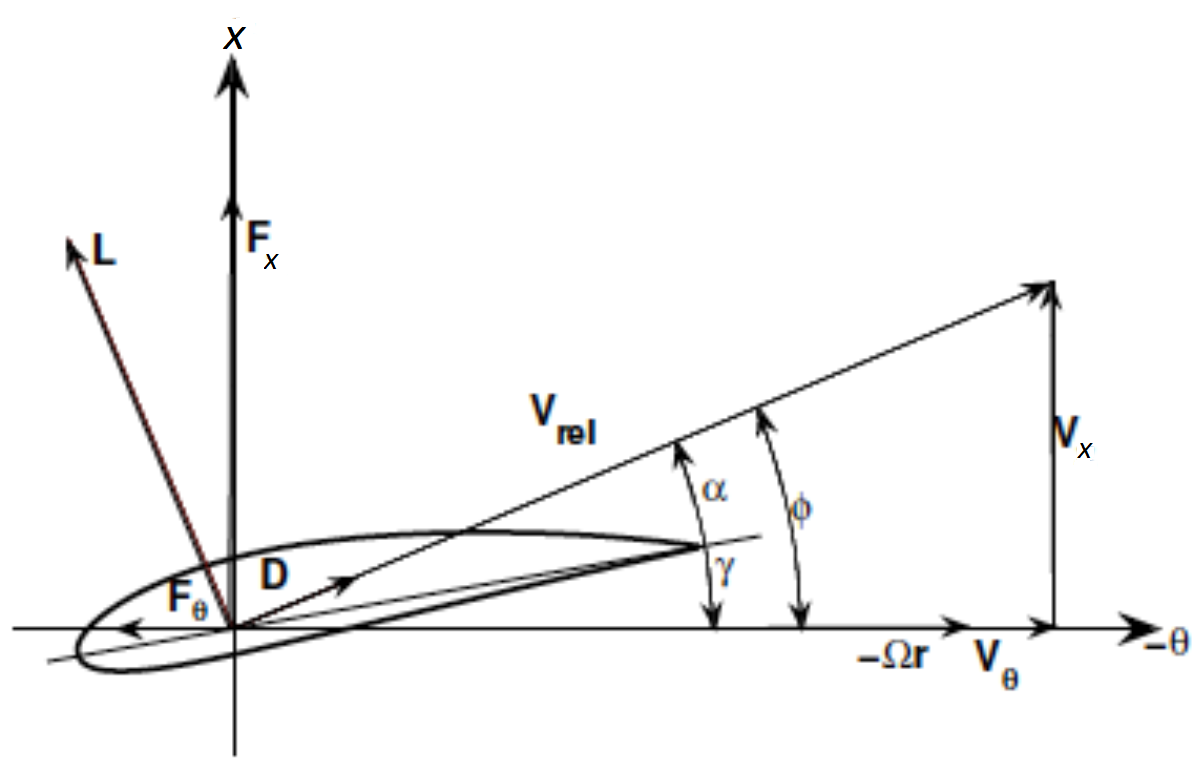
\includegraphics[width=0.45\textwidth]{Figure/triangle.png}\\
 \caption[Velocity triangle on a wind turbine blade]{Velocity triangle for the determination of the local relative velocity on a turbine blade.}
 \label{f:triangle}
\end{figure}
After calculating the local aerodynamic force $\vec{f}= L\vec{e_L}+D\vec{e_D}$, its influence, $-\vec{f}$, on the flow is incorporated as a sum of discrete forces (here $\vec{e_L}$ and $\vec{e_D}$ are the unit vectors in the direction of the local lift and drag, respectively). The total force from all the blade elements experienced by the fluid is given by
\begin{equation}
\vec{F}(x,\,y,\,z,\,t)=-\sum_{i=1}^{N}\vec{f}(x_i,\,y_i,\,z_i,\,t)\,\delta(|\vec {r}-\vec{r_i}|) \label{force}
\end{equation}
where, $\delta(|\vec {r}-\vec{r_i}|)$ is the Dirac delta function. Equation(\ref{force}) represents the discrete force model in a continuous form by using delta function. To avoid  singularities, the forces are distributed smoothly on several mesh points by using the Gaussian weight function (smeared out delta function),
\begin{equation}
\eta_{\,\epsilon}(d)=\frac{1}{\epsilon^3\pi^{3/2}}\exp\big[-\big(\frac{d}{\epsilon}\big)^2\big],
\end{equation}
with the modified force term as
\begin{equation}
\vec{F}(x,\,y,\,z,\,t)=-\sum_{i=1}^{N}\vec{f}(x_i,\,y_i,\,z_i,\,t)\,\eta_{\,\epsilon}(|\vec {r}-\vec{r_i}|),
\end{equation}
where the summation is over all $N$ blade elements, $x_i,y_i,z_i$ are the local coordinates of each blade element, and $|\vec {r}-\vec{r_i}|$ is the distance between the current point in the flow and the center of the blade element. Several studies have been carried out for the choice of an optimal Gaussian width $\epsilon$~\cite{troldborg, martinez}. The value of $\epsilon=2\,w$ proposed by Troldborg~\cite{troldborg} is used in the current study.




 

\chapter{Results: Precursor Simulation} % Main chapter title

\label{Chapter3} % For referencing the chapter elsewhere, use \ref{Chapter1} 

\lhead{Chapter 3. \emph{Results: Precursor Simulation}} % This is for the header on each page - perhaps a shortened title
%----------------------------------------------------------------------------------------
In the current chapter we report the computational domain and the results of the precursor simulation to the wind turbine array, which in this case is neutral atmospheric boundary layer at very high $Re$ and single wind condition. A rigorous parametric study has been performed on the subgrid-scale model as well as on the near wall modelling paramters, and the best model has been chosen based on the analysis of the results that will be used subsequently in all the models involving wind turbine array simulation. The proper knowledge of ABL precursor simulation is necessary since it is being used as a realistic inflow condition to drive flow past wind turbine arrays. 
\section{Computational Domain}
 The computational domain for ABL simulation has been chosen to be $L_x = 2\pi H$, $L_y = \pi H$ and $L_z = H$ ({where $H$ is the} BL thickness). The Reynolds number chosen for the current computation is $Re = 10^{10}$ with the length scale of $H$ and the bulk velocity scale $U_m$. The choice of the streamwise extent is crucial since it should be large enough such that the auto-correlation length scale decays significantly to make the periodic boundary conditions consistent~\cite{kimmoinmoser,pope,hoyas}. Previous literature in channel flow and ABL flow simulations have reported streamwise {\&}  spanwise geometry in terms of multiples of boundary layer thickness respectively as $2\pi \ \& \ \pi$ ~\cite{kimmoinmoser,porte1a,meyers2}, $2\pi \ \& \ 2\pi/3$~\cite{porte2a} with {perhaps the largest domain}  reported as $2\pi \ \& \ 2\pi$~\cite{porte1fun} . {We have considered the smallest domain possible to optimise the computational expense and simultaneously the insensitivity of the results on two different domains $2\pi H \times 2\pi H \times H$ \& $2\pi H \times \pi H \times H$  (not reported here) are observed as well.} . The aerodynamic roughness is $z_0 = 10^{-4}H$, similar to the past literature~\cite{porte2a,meyers2}. The discretization parameters of the {baseline domain} are tabulated below.  $N^{e}_i$ represents the number of elements in the $i^{th}$ direction while $\Delta_x, \ \Delta_y, \ \Delta_z$ are the minimum grid sizes of the GLL nodes {across all the elements}. Table~\ref{table:grid1}  reveals the anisotropy of the streamwise grids ($\Delta_x/\Delta_z, \ \Delta_x/{\Delta_y}$) with respect to the wall normal and spanwise grid {sizes} in the near wall region which conforms well with the past literature~\cite{pio2,meyers2}. {The minimum grid point wall-normal distance }$ \Delta z/z_0 \gtrapprox 25$ manifesting the first grid node does not resolve the geometric roughness and lies in the log-law of the wall ~\cite{meyers2} (The grid designed for the current $ABL$ is supposed to be in the high-accuracy zone of $\mathfrak{R}-{Re}_{LES}$ space as discussed by Brasseur and Wei, and so there is technically no necessity of a grid convergence test, see ~\cite{brass} and Section~\ref{lotw} for details). \\
\begin{table}[ht] 
\centering % used for centering table 
\begin{tabular}{c c c c c} % centered columns (4 columns) 
\hline\hline    %inserts double horizontal lines 
Geometry & $N^{e}_x\times N^{e}_y\times N^{e}_z$  & $\Delta_x/\Delta_z$ & $\Delta_x/\Delta_y$ & $\Delta z/z_0$  \\ [0.5 ex] % inserts table 
%heading 
\hline  % inserts single horizontal line 
$2\pi H \times \pi H \times H$ & $30\times 20\times 24$ & $4.98$ & $4.11$ & $27.88$ \\ [1ex] % inserting body of the table 
\hline\hline \\ [1 ex]
\end{tabular} 
\caption[Computational Grid in ABL]{Numerical setup for ABL LES for {the baseline grid}} % title of Table 
\label{table:grid1} % is used to refer this table in the text 
\end{table} 
  The order of the polynomial{s} chosen for the present purpose is $N = 7$, which is near optimum~\cite{nek5000} since with low values of $N\sim 4-6$, the effects of dissipation and dispersion errors start creeping in, and using higher-order polynomials $N\sim 10-12$ increases the computational cost significantly without improving on the accuracy of LES results which {at the high resolution of $N\geq 7$} are mainly due to SGS modelling errors.
\section{Results and Discussion}\label{results}
{In this section, the LES simulation results for different parametric tests {are} presented and benchmarked with the past literature with a rigorous analysis on the observed results in order to comment on the robustness of the model. 
%To ensure a cleaner perspective, at the very beginning we present
{In Table~\ref{table:sim}, we summarize} the different simulations {that were} performed in order to carry out a parametric analysis of the LES model comparing the results of the statistics.}.   
\begin{table}[ht] 
\centering % used for centering table 
\begin{tabular}{c c c c} % centered columns (4 columns) 
\hline\hline    %inserts double horizontal lines 
Case & $k_c$  & Interpolation & $\lbrace C_0, \ n \rbrace$   \\ [0.5 ex] % inserts table 
%heading 
\hline  % inserts single horizontal line 
I & $1$ & $M$ & $\lbrace 0.16, 2 \rbrace$ \\
II & $2$ & $M$ & $\lbrace 0.16, 2 \rbrace$ \\
III & $4$ & $M$ & $\lbrace 0.16, 2 \rbrace$ \\  % inserting body of the table 
IV & $6$ & $M$ & $\lbrace 0.16, 2 \rbrace$ \\
\hline
V & $2$ & $M$ & $\lbrace 0.17, 1 \rbrace$ \\
VI & $4$ & $M$ & $\lbrace 0.17, 1 \rbrace$ \\
VII & $6$ & $M$ & $\lbrace 0.17, 1 \rbrace$ \\
\hline

VIII & $2$ & $M$ & $\lbrace 0.19, 0.5 \rbrace$ \\
IX & $4$ & $M$ & $\lbrace 0.19, 0.5 \rbrace$ \\
X & $6$ & $M$ & $\lbrace 0.19, 0.5 \rbrace$ \\
\hline
XI & $4$ & $M$ & $\lbrace 0.16, 3 \rbrace$ \\
\hline
XII & $4$ & $S$ & $\lbrace 0.19, 0.5 \rbrace$  \\
\hline \\ [1 ex]
\end{tabular} 
\caption[Cases in ABL simulation]{12 LES cases run for neutral ABL flows. $k_c$: cut-off filter in explicit filtering of NWM. $M$ denotes mid point $\&$ $S$ denotes spectral interpolation in approximate BC. $\lbrace C_0, \ n \rbrace$: tuning parameters of SGS model. } % title of Table 
\label{table:sim} % is used to refer this table in the text 
\end{table} 

{{As can be seen from} Table~\ref{table:sim}, {in line with the discussion in Section 2.2}, the major parametric stud{ies} that we want to perform in the current section are {on} the effect of the filtering on near wall modelling (different values of $k_c$) as well as the shape of the SGS mixing length parameter (tuning parameters $C_0, n$).}  The results of the various simulation cases presented in this chapter for comparison are mainly $(a)$ {Mean streamwise velocity gradient} (b) Mean resolved turbulent stresses $(c)$ {Mean resolved 1D \& 2D spetra of streamwise energy, \& enstrophy }. In the current section, results of the mean statistics are presented and compared against the dynamic models of Porte-Ag\'{e}l et al.~\cite{porte1fun}, {and the implications of results are analyzed}.
% along with their implications using rigorous analysis.
\subsection{Subgrid scale and Near Wall modelling effects on Log Law}
\begin{figure}
\centering
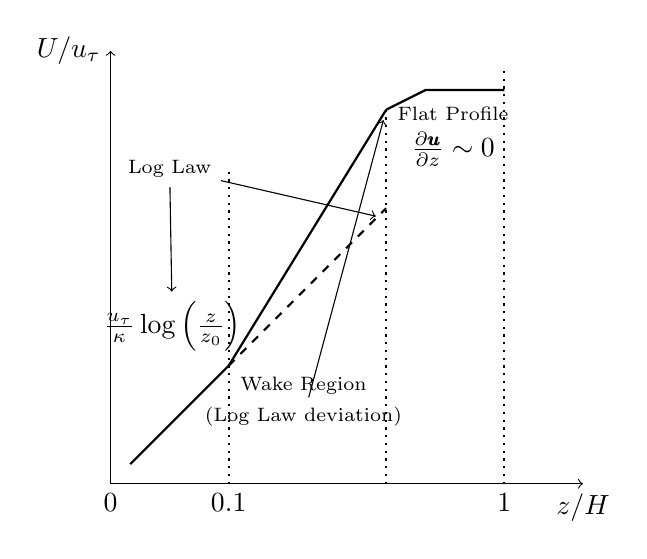
\begin{tikzpicture}[out=0,in=180,relative]

% horizontal axis
\draw[->] (0,0) -- (6,0) node[anchor=north] {\normalsize ${z}/{H}$};
% labels
\draw	(0,0) node[anchor=north] {0}
		(1.5,0) node[anchor=north] {0.1}
		(3.5,0) node[anchor=north] {}
		(5,0) node[anchor=north] {1};
% ranges
%\draw	(1,3.5) node{{\scriptsize Constant flux}}
%		(4,3.5) node{{\scriptsize Field weakening}};

% vertical axis
\draw[->] (0,0) -- (0,5.5) node[anchor=east] {\normalsize ${{U}}/{u_{\tau}}$};
% nominal speed
\draw[thick,dotted] (1.5,0) -- (1.5,4);

% Us
\draw[thick] (0.25,0.25) -- (1.5,1.5) node (a_2b) {};
\draw[thick,dashed] (1.5,1.5) -- (3.5,3.5) node[anchor=north] (a_2) {};
%\draw[->] (0.25,0.25) -- (1.5,1.5)

%\draw (1,1.5) node {$U_s$}; %label

% Us
\draw[thick] (1.5,1.5) -- (3.5,4.75);
%\draw (2,1.5) node {$U_s$}; %label
\draw[thick,dotted] (3.5,0) -- (3.5,4.75) node (a_2c) {};;

% Psis
\draw[thick] (3.5,4.75) -- (4.0,5) parabola[bend at end] (5,5);
\draw[thick,dotted] (5,0) -- (5,5.25);

\draw (0.75,4) node (a) {\scriptsize Log Law}; %label
\draw (0.785,2) node (b) {\normalsize $\frac{u_{\tau}}{\kappa}\log \left(\frac{z}{z_0}\right)$}; %label
\draw (2.45,1.25) node (c) {\scriptsize Wake Region}; %label
\draw (2.45,0.85) node (c) {\scriptsize (Log Law deviation)}; %label
\draw (4.35,4.7) node (d) {\scriptsize Flat Profile}; %label
\draw (4.35,4.25) node {\normalsize $\frac{\partial \pmb{u}}{\partial z} \sim 0$}; %label

\path[->] (a) edge (b)
              edge (a_2) ;
              
\path[->] (c) edge (a_2c);  
\end{tikzpicture}
\caption[Schematic of Log-Law of wall]{Schematic of log law of the wall over a rough wall for high Reynolds number. The $x$ axis is in log-scale. Within $z/H \lessapprox 0.1$, logarithimic trends observed: LOTW (Law of the Wall); beyond $z/H \sim 0.1$, log-law deviation: ``wake layer"; $z/H \sim O(1)$, $U(y)$ gradually becomes flatter, $\frac{dU}{dz} \approx 0$, at top lid - symmetry boundary conditions. (See ~\cite{pio2,porte1fun,meyers2} for details in LOTW)}           \label{fig:schematic}
\end{figure}
For first order statistics, velocity $U${(z)} is the temporal{ly} and horizontally averaged (homogeneous $x-y$ plane) streamwise mean velocity profile ${\langle \overline{\widetilde{u}}\rangle_{xy}}$. All the plots involving physical length scale $z$ has been normalized with the boundary layer thickness $H$. The temporal average has been taken for 10 sweeps of ``flow-through" time scale $L_x/U_{bulk}$ which is consistent with the literature ~\cite{kimmoinmoser}. We expect the streamwise mean velocity profile {at the lower $10-20 \%$ of the boundary layer ($z/H \sim 0.1-0.2$) to follow the logarithmic trend ($\Phi(z) = \kappa z/u_{\tau} dU/dz = 1$), deviate from the log-law ($\Phi(z) > 1$) beyond $x/H \sim 0.2$, popularly known as the ``wake-region" and a small flat region where the gradient gradually approaches zero due to the top symmetry boundary conditions. (See schematic in Figure~\ref{fig:schematic})} In the near-wall region, $z/H \sim 0.1$, $$\frac{{U(z)}}{u_{\tau}} = \frac{1}{\kappa}\log (\frac{z}{z_0}) = \frac{1}{\kappa}\log (\frac{z}{H}) + \frac{1}{\kappa}\log (\frac{H}{z_0}) = \frac{1}{\kappa}\log (\frac{z}{H}) + C \ ,$$ constant $C$ being a function of the roughness parameter. {From the perspective of physics, $C$ should be a function of $f(H/z_0)$, the two relevant scales of high $Re$ ABL; however with different tuning parameters $C_0, \ n$ of the SGS model, it is observed that $C \approx f(H/z_0; C_0,n)$ as is manifested also in the numerical model.}  
%The quantified effect of $C_0, \ n$ on $C$ is beyond the scope of the present paper, and is anticipated to be addressed in a separate article. 
Consequently, to understand the effect of SGS stresses on the log-law of the wall explicitly, yet decouple (atleast partially) the implicit effect of SGS stress on the mean velocity profile through $C$, metric in the form of non-dimensional mean velocity gradient $\Phi = \frac{\kappa z}{u_{\tau}} dU(z)/dz$ is more favourable since parametric constant $C$ can be eliminated with the use of derivatives.\\
 With $Re \sim 10^{10}$, eddy-viscosity in the current LES model results in $\nu_{t} (= (C_s\Delta)^2 \vert \widetilde{S} \vert) \gg \nu \approx 0$ which indicates the kinematic shear stress in an LES framework for a flat-plate type geometry can be given as
  \begin{align}
-\overline{\widetilde{u'}\widetilde{w'}} + \langle\overline{\nu_{t}} \rangle_{xy} \frac{d U}{d z} \approx \frac{\tau_{w}}{\rho}\left(1 - \frac{z}{H}\right). \label{mean}
\end{align}
Equation(~\ref{mean}) shows that the total stress is perfectly linear which has been reported in previous literature~\cite{kimmoinmoser,brass}.
From Equation~(\ref{mean}) (both RHS and LHS are {only} function{s} of $z$ due to homogeneity in the $xy$ direction), we obtain an estimate of the non-dimensional mean velocity gradient $\Phi(z)$ as 
\begin{equation}
\Phi(z) = \frac{\kappa z}{u_{\tau}}\frac{dU}{dz} = \frac{u_{\tau}\kappa z}{(C_s\Delta)^2 \langle \vert \widetilde{S} \vert)\rangle_{xy}}\left(1 - \frac{z}{H} + \frac{\overline{\widetilde{u'}\widetilde{w'}}(z)}{{u_{\tau}}^2}\right)
\end{equation}
, which can be further simplified as
\begin{equation}
\boxed{\Phi(z) = \frac{\kappa z}{C_s \Delta} \times \frac{u_{\tau} f(z)/ \langle\vert \widetilde{S} \vert)\rangle_{xy}}{C_s \Delta}} = A_1(z)\times A_2(z), \label{mean2b}
\end{equation}
with $f(z) = (1 - z/H + \overline{\widetilde{u'}\widetilde{w'}}/u_{\tau}^2)$ being a non-dimensional function of $z$ and $u_{\tau} = \sqrt{\tau_{w}/\rho}$. Also, it is important to note that the shear stress boundary condition is essentially a reflection of the log-law of the wall in its time averaged form (See Equation~(\ref{stress2})) which manifests $u_{\tau} = f(\widehat{\widetilde{u}_r})$ from the approximate stress boundary conditions.

It is quite straightforward to see the contributions of SGS stress and approximate stress boundary conditions {to} the non-dimensional mean velocity gradient $\Phi(z)$. {Close to the wall, the standard Smagorinsky damps the filter length scales retrieving log-law of rough wall $C_s\Delta \sim \kappa (z + z_0) \approx \kappa z$.} . The eddy turn over time of the near wall eddies {can be defined as} $t_{eddy} \sim f(z)/\langle\vert \widetilde{S} \vert\rangle_{xy}$ ({from now on,} we will use just $\widetilde{S}$ instead of $\langle\vert \widetilde{S} \vert\rangle_{xy}$ for brevity, statistical $x{y}$ directional homogeneity is implied). Since the near wall eddies are mostly subgrid scale and need to be modelled, it is not hard to relate  the eddy-turn over time of the near wall ``subgrid-eddies" with the so called {mixing length scale of eddies and they should correspond well with the Smagorinsky length scale $C_s \Delta$}.{It is thus important to realize that $\Phi (z)$ corresponding to the log-law, would potentially generate a value of 1 near wall, if trivially $A_1(z), \ A_2(z)$ are 1.}   

{It must be understood that, the \textbf{above conditions are ideal} from the perspective of physics just to give an example to the reader}. However, due to the smoothing effect of blending function in the wall-damped Smagorinsky model, the filter length scale close to the wall  $l_f = C_s\Delta$ may deviate from $\kappa z$ ($A_1 \neq 1)$ ; {may not be exactly $1$ in the near wall region, and it is the responsibility of the numerics to capture $u_{\tau}$ from the stress boundary conditions properly so as to alter the eddy mixing length $u_{\tau} t_{eddy}$, in an effort to make $A_1(z) \times A_2(z) = 1 $}.  

{From the perspective of physics, it is quite apparent that the standard Smagorinsky with wall damping by Mason and Thompson~\cite{mason} which retrieves log law scale near wall is potentially as consistent as its dynamic counterpart (standard/scale dependant) in the near wall regime (at least in the horizontally homogeneous problem) which are based entirely on mathematical empiricism (e.g. scale invariance or power law dependance of $C_s\Delta$) as presented in the previous literature~\cite{germano,porte1fun,bou1}.}  

{We would discuss these formulations in the later half of the section again corroborated by respective plots.
Hence, to summarize, the Results section would not only comprize of the \textit{first and second order statistics} but also \underline{some additional plots} commenting on the errors of $A_1(z)$ and $A_2(z)$ to corroborate the analytical predictions regarding the law of the wall and turbulence production as discussed in the previous paragraphs.}  .
\subsection{Cases I-IV}
To start with, we present the results of simulations $I-IV$ in Figures~\ref{fig:stata},~\ref{fig:stat21},~\ref{fig:stat22}. They involve statistics for different values of the filter cut-off wave-numbers $k_{c}$ (See Appendix~\ref{elfilt} for details)  with fixed parameters $n = 2, \ C_0 = 0.16$ for Standard Smagorinsky model using mid-point interpolation for approximate stress boundary condition (Refer to Section~\ref{nwm}). Figure~\ref{fig:stata} depicting mean velocity gradient shows a reasonable match with the standard Smagorinsky results of previous literature. It is interesting to see the region of "log-layer mismatch" corresponding to $\Phi(z) \approx 1.4$ (maximum 40 \% error near wall) in the lower $10\%$ of the ABL predicting similar trends to the results of Bou-Zeid et. al~\cite{bou1}. In fact previous standard Smagorinsky based LES results from Sullivan et. al~\cite{sull} and Chow et. al~\cite{chow} show similar trends of log-layer mismatch in the near wall region as shown in Figure~\ref{fig:sulchow}. The effect of filtering is {nearly} indistinguishable in the region $z/H \sim 0.1$, but conspicuous differences can be observed {at $z/H \gtrapprox 0.3$.}
% in the outer layer ($z/H \gtrapprox 0.5$). 
{Even though $k_c = 6$ shows quite {a} good match with the standard Smagorinsky counterpart~\cite{bou1} in the outer layer ($z/H > 0.3$), the results by $k_c = 1, 2, 4$ shows some reminiscent effect of logarithmic trends in lower $15-20 \%$ of the boundary layer~\cite{meyers2} and more prominent deviations into the ``wake region".} 

The results of second order statistics in Figures~\ref{fig:stat21},~\ref{fig:stat22} show that $k_c = 2,4$ has the best match with the standard Smagorinsky results of Porte-Ag\'{e}l et. al~\cite{porte1fun} except that the peaks of \textit{$v_{rms}$ and $uw_{rms}$}  are slightly over-predicted with respect to ~\cite{porte1fun} {but} the peak locations remain {similar}. {In general the stresses with $k_c = 6$ show significant effects of dissipation, resulting in smaller values of peaks for the Reynolds stresses compared to the other values of the filter parameter $k_c$}. For the kinematic shear stress $-uw_{rms}$, the near wall behaviour ($z/H \lessapprox 0.1$) of $k_c = 6$ is similar to standard Smagorinsky, while $k_c=2, 4$ has similitude with its scale dependant counterpart. It is important to mention that the location of the Reynolds-stress peaks are unchanged by the process of filtering ($k_c = 2, 4, 6$). 
\begin{figure}
\centering
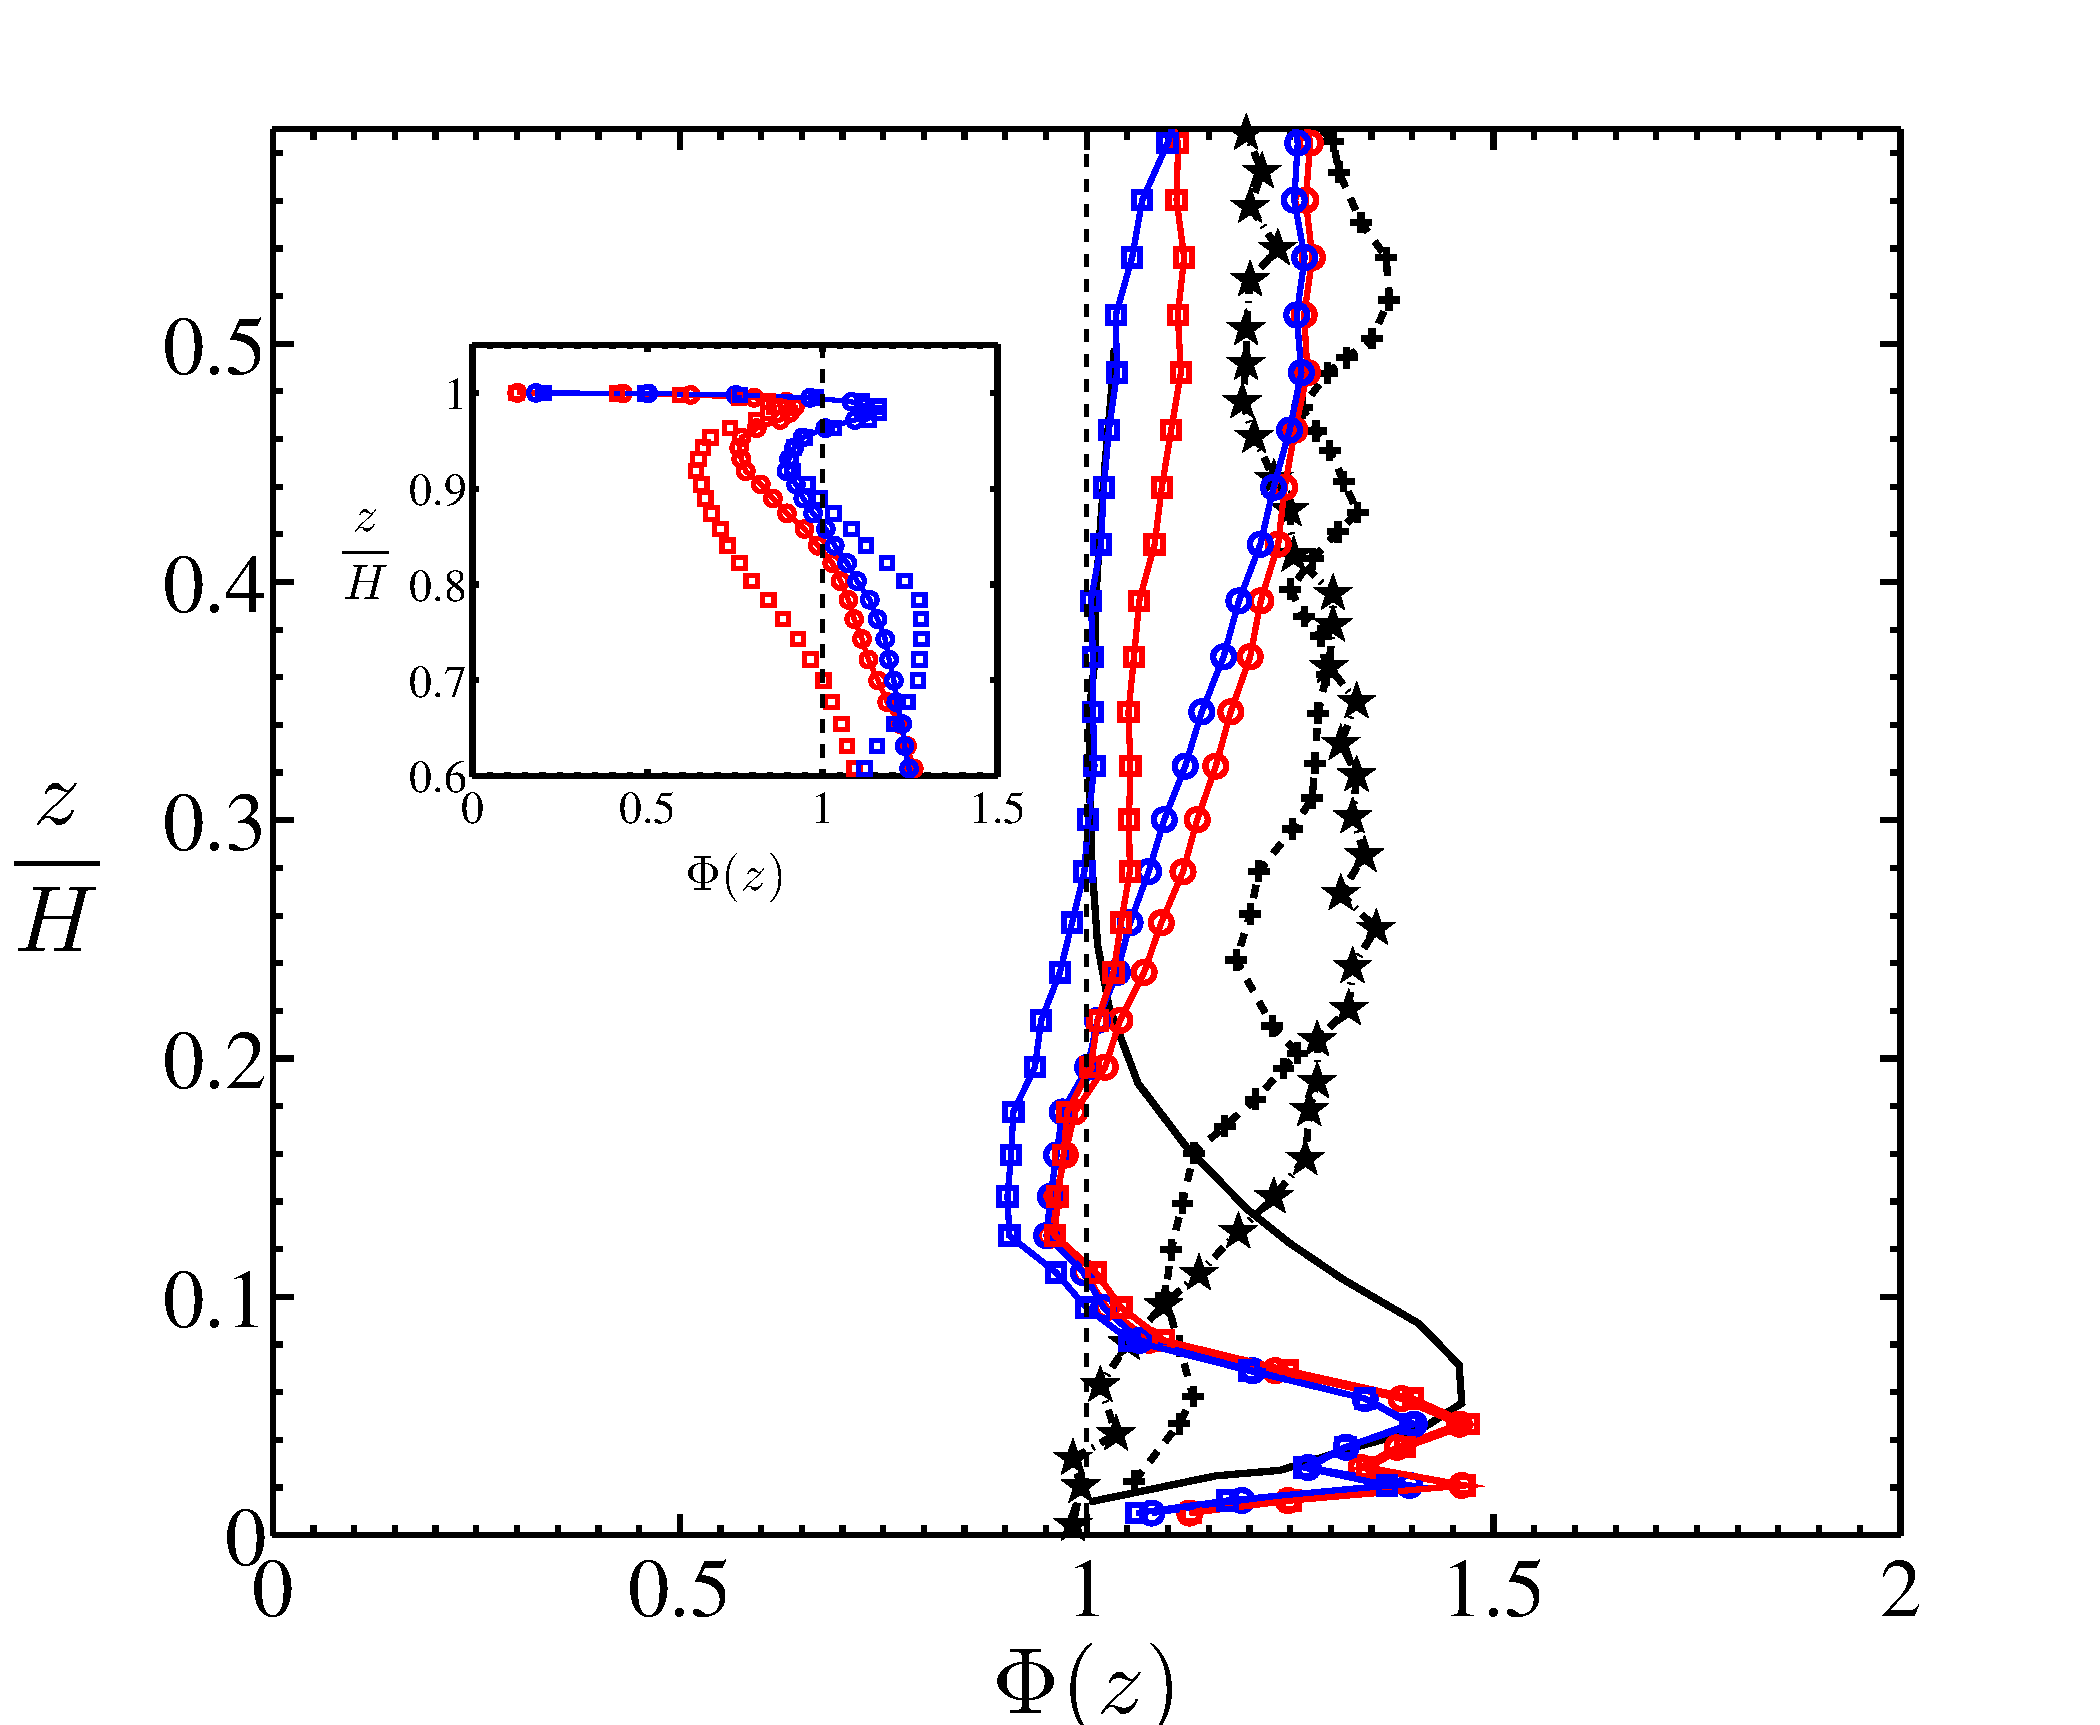
\includegraphics[width = 0.75\linewidth]{Fig3/gradient_filt_n2.pdf}        
        \caption[$\Phi(z)$, Case $I-IV$]{Non dimensinonal mean streamwise velocity gradient $\phi(z)$ vs $z/H$. Red, Blue curves: current simulations $I-IV$ ($n = 2, \ C_0 = 0.16$); Black curves from the literature~\cite{porte1fun,bou1}. Red $\Box$, $k_{c}=1$; $\circ$, $k_{c}=2$; Blue $\circ$, $k_{c} = 4$; Blue $\Box$, $k_{c} = 6$. Black $+$ scale dependant dynamic Smagorinsky for Port$\acute{e}$-Agel et al.~\cite{porte1fun}; $-$ , standard Smagorinsky, Bou-Zeid et. al, $\star$, Lagrangian scale dependant dynamic Smagorinsky with filtering, Bou-Zeid et. al~\cite{bou1}.}\label{fig:stata}
\end{figure}

\begin{figure}
\centering
        \begin{subfigure}[t]{0.42\textwidth}
                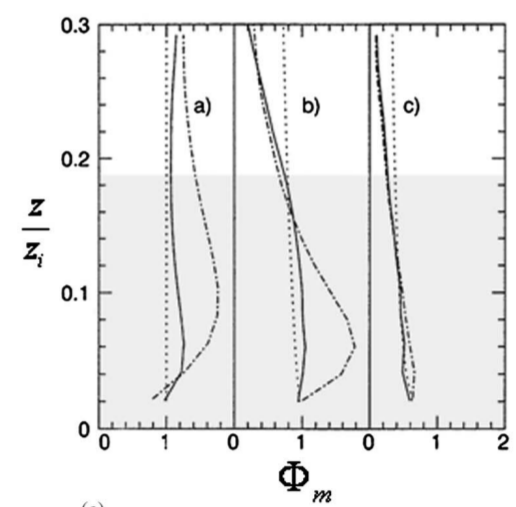
\includegraphics[width=\linewidth]{Figure/sullivan.png}
                \caption{}
                \label{fig:phi1}
        \end{subfigure}%
        \centering
        \begin{subfigure}[t]{0.475\textwidth}
                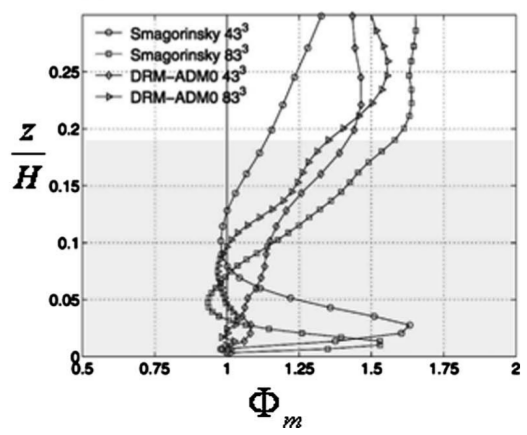
\includegraphics[width=\linewidth]{Figure/chow.png}
                \caption{}
                \label{fig:phi2}
        \end{subfigure}%
        \caption[Law of Wall: Previous studies]{Non dimensinonal mean streamwise velocity gradient $\phi(z)$ vs boundary layer height in previous LES studies (standard Smagorinsky). (a) Sullivan et. al~\cite{sull}; $z_i$ is the conventional ABL depth used {in the} atmospheric community as the height where vertical turbulent heat flux is a minimum. (b) Chow et. al~\cite{chow} uses similar simulations as in the current results without capping inversion. The plots are taken from Brasseur and Wei~\cite{brass}}\label{fig:sulchow}
\end{figure}
\begin{figure}
\centering
        \begin{subfigure}[t]{0.75\textwidth}
                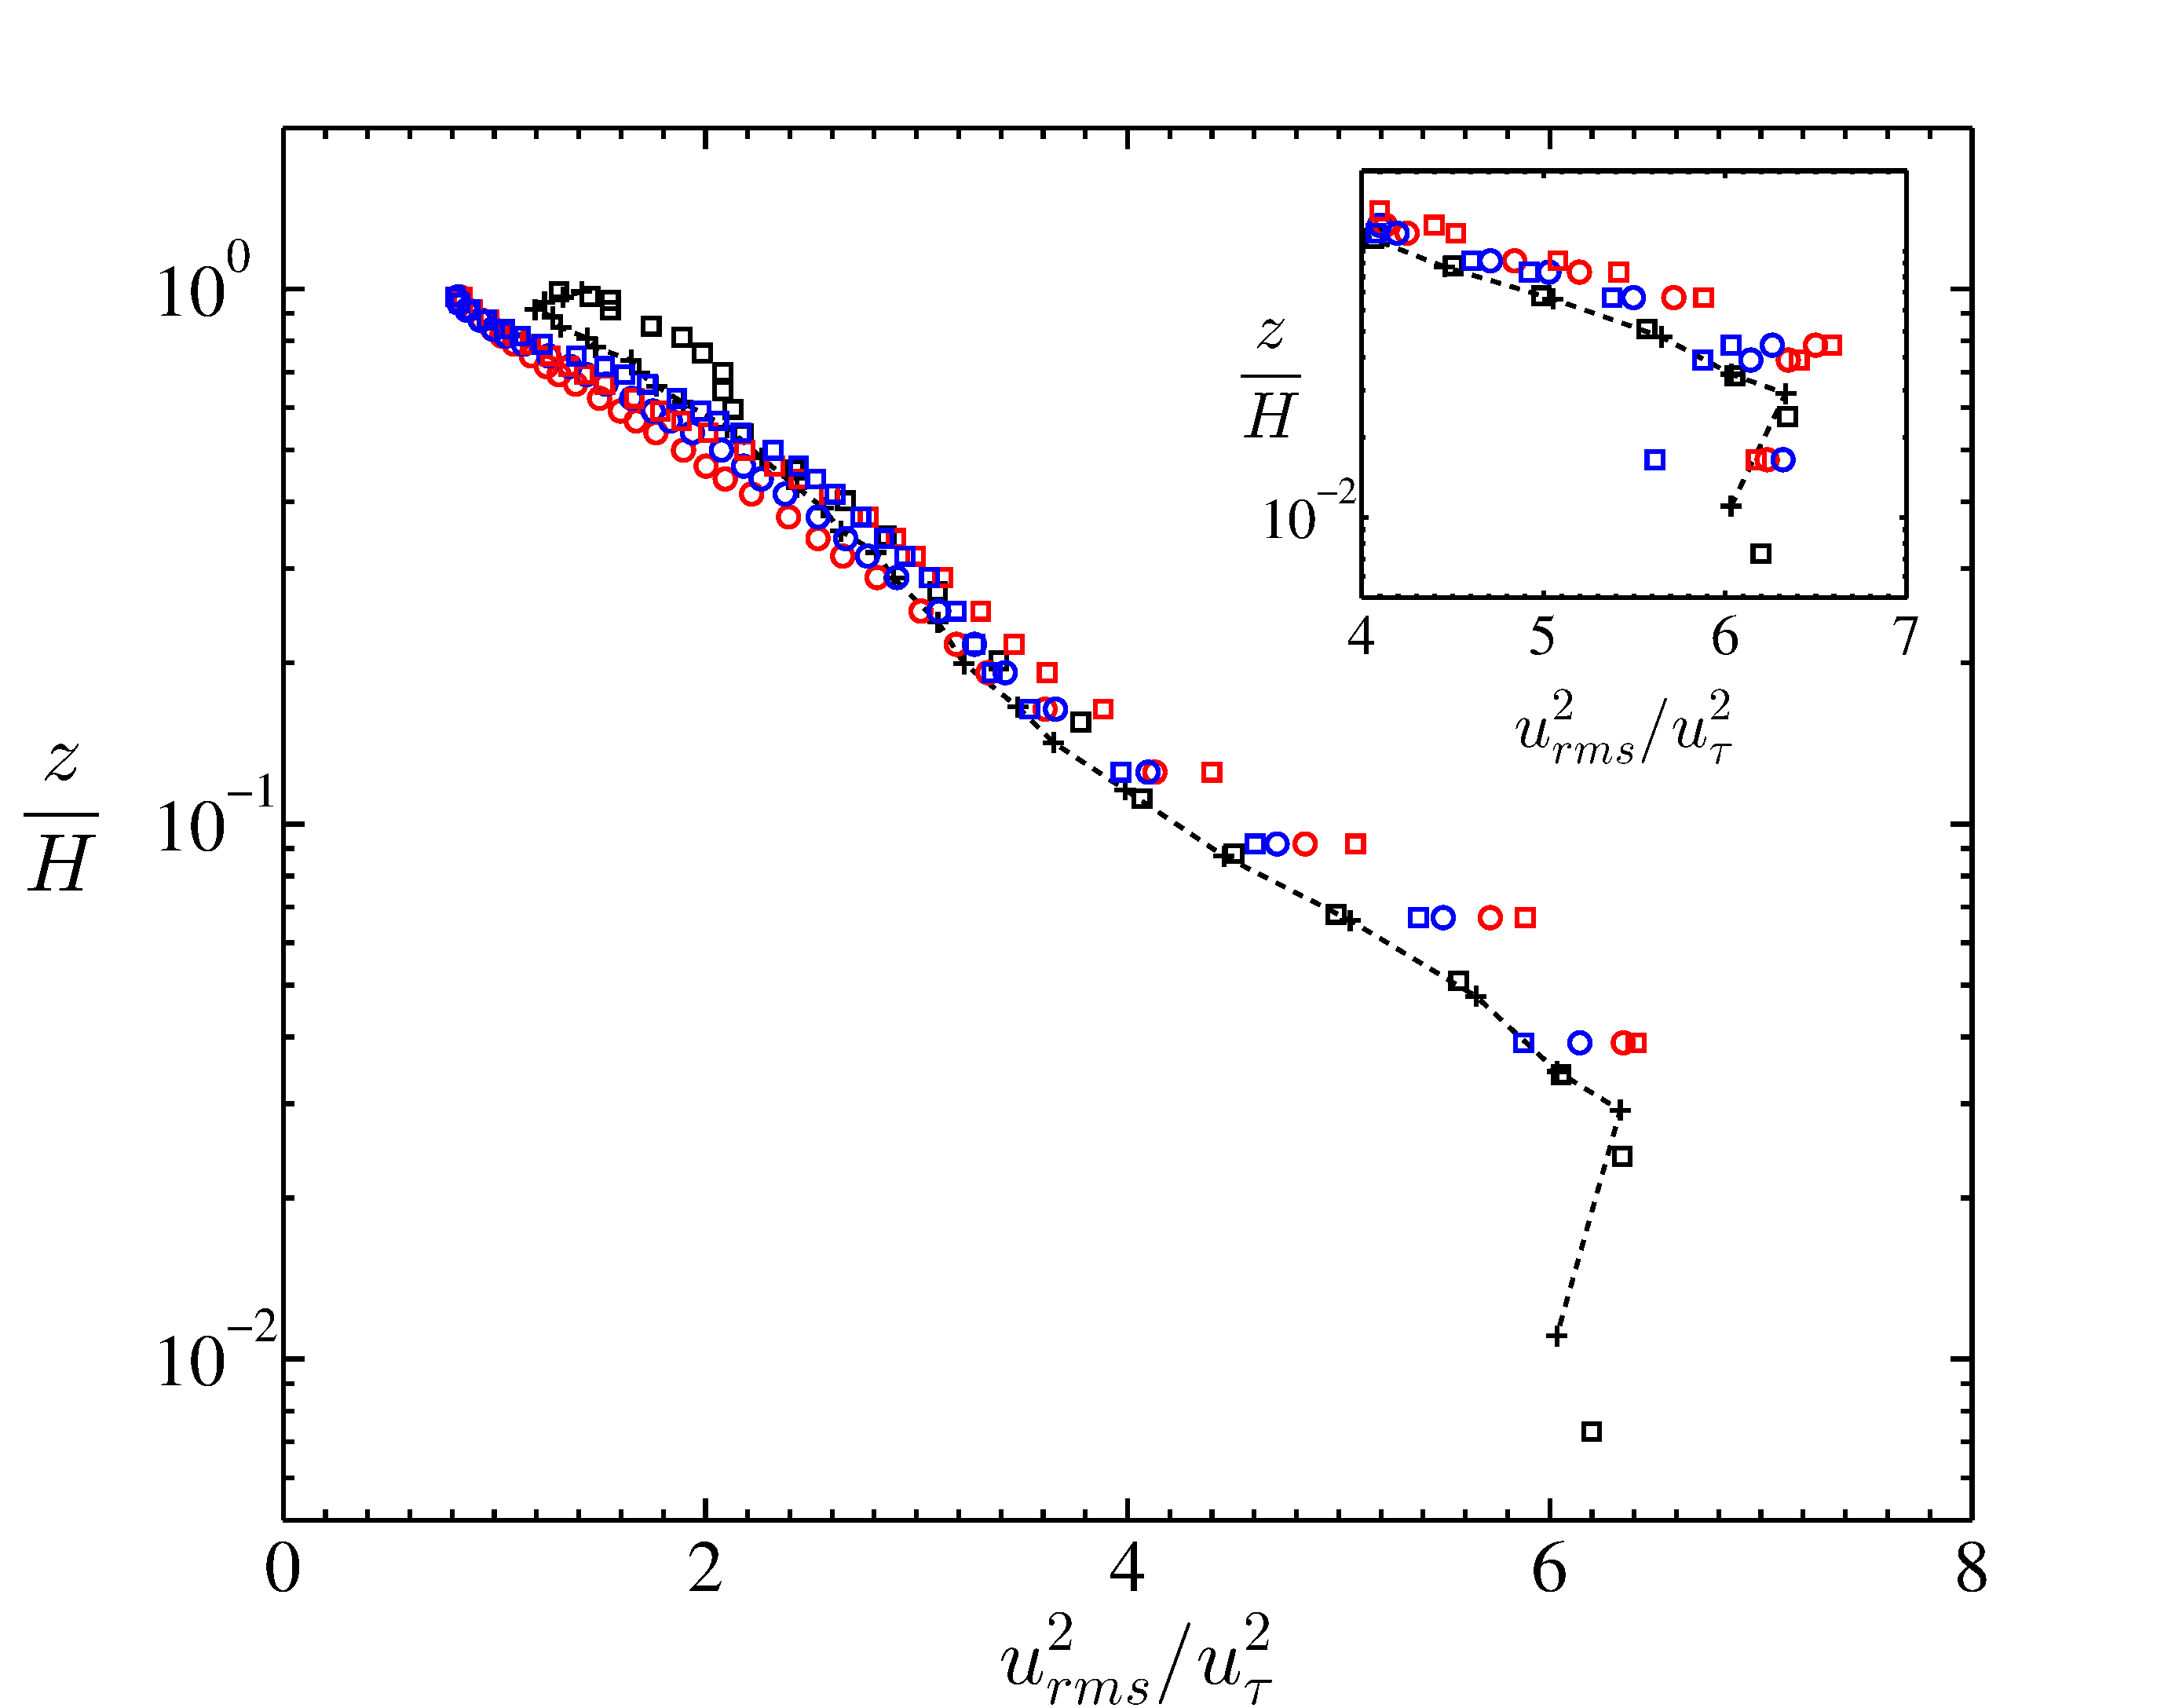
\includegraphics[width=\linewidth]{Fig3/urms_filter_n2.pdf}
                \caption{}
                \label{fig:urms}
        \end{subfigure}
        \centering
        \begin{subfigure}[t]{0.75\textwidth}
                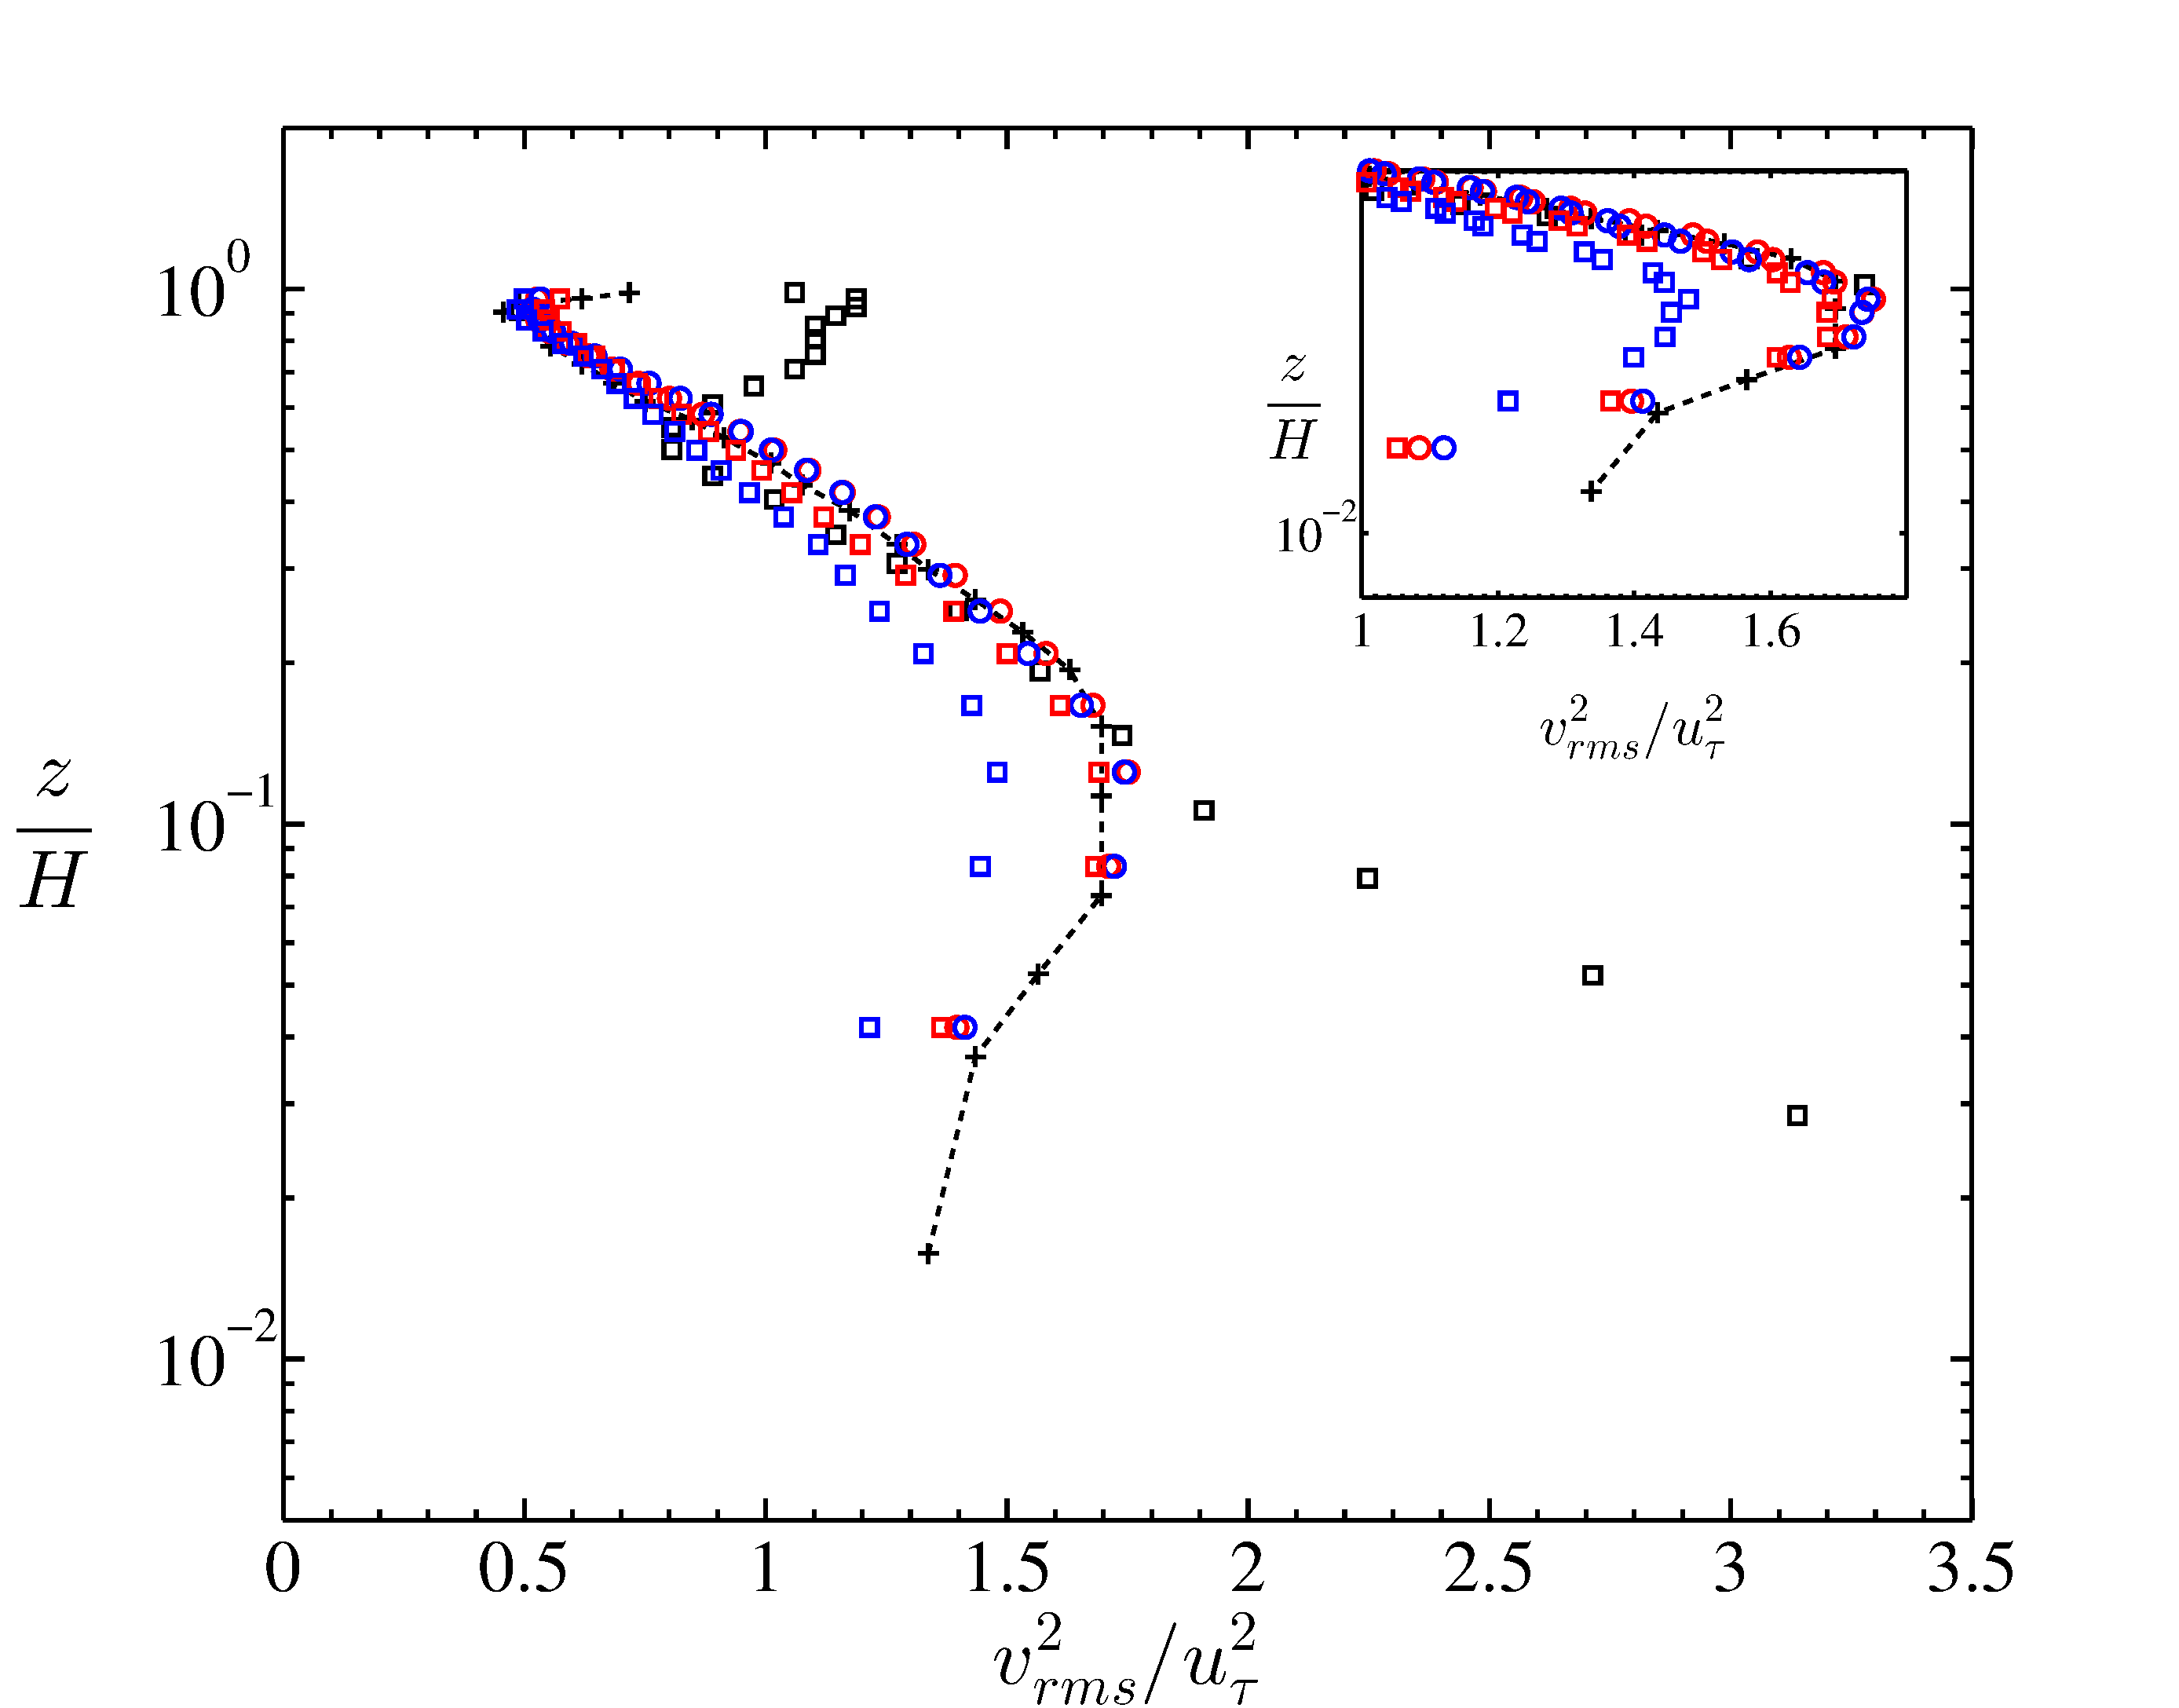
\includegraphics[width=\linewidth]{Fig3/vrms_filter_n2.pdf}
                \caption{}
                \label{fig:vrms}
        \end{subfigure}
        \caption[Second order statistics $u_{rms}, \ v_{rms}$, Case $I-IV$]{Second order statistics for ABL simulations: Case $I-IV$. (a) $u_{rms}$ (b) $v_{rms}$. Red, Blue curves: current simulations $I-IV$ ($n = 2, \ C_0 = 0.16$);  Red $\Box$, $k_{c}=1$; $\circ$, $k_{c}=2$; Blue $\circ$, $k_{c} = 4$; Blue $\Box$, $k_{c} = 6$.  Black $-+$, standard Smagorinsky ($C_s = 0.10, n = 2$) {for Port$\acute{e}$-Agel et al.~\cite{porte1fun}} and black $\Box$ scale dependant dynamic Smagorinsky for Port$\acute{e}$-Agel et al.~\cite{porte1fun}}\label{fig:stat21}
\end{figure}
\begin{figure}        
        \centering
        \begin{subfigure}[t]{0.75\textwidth}
                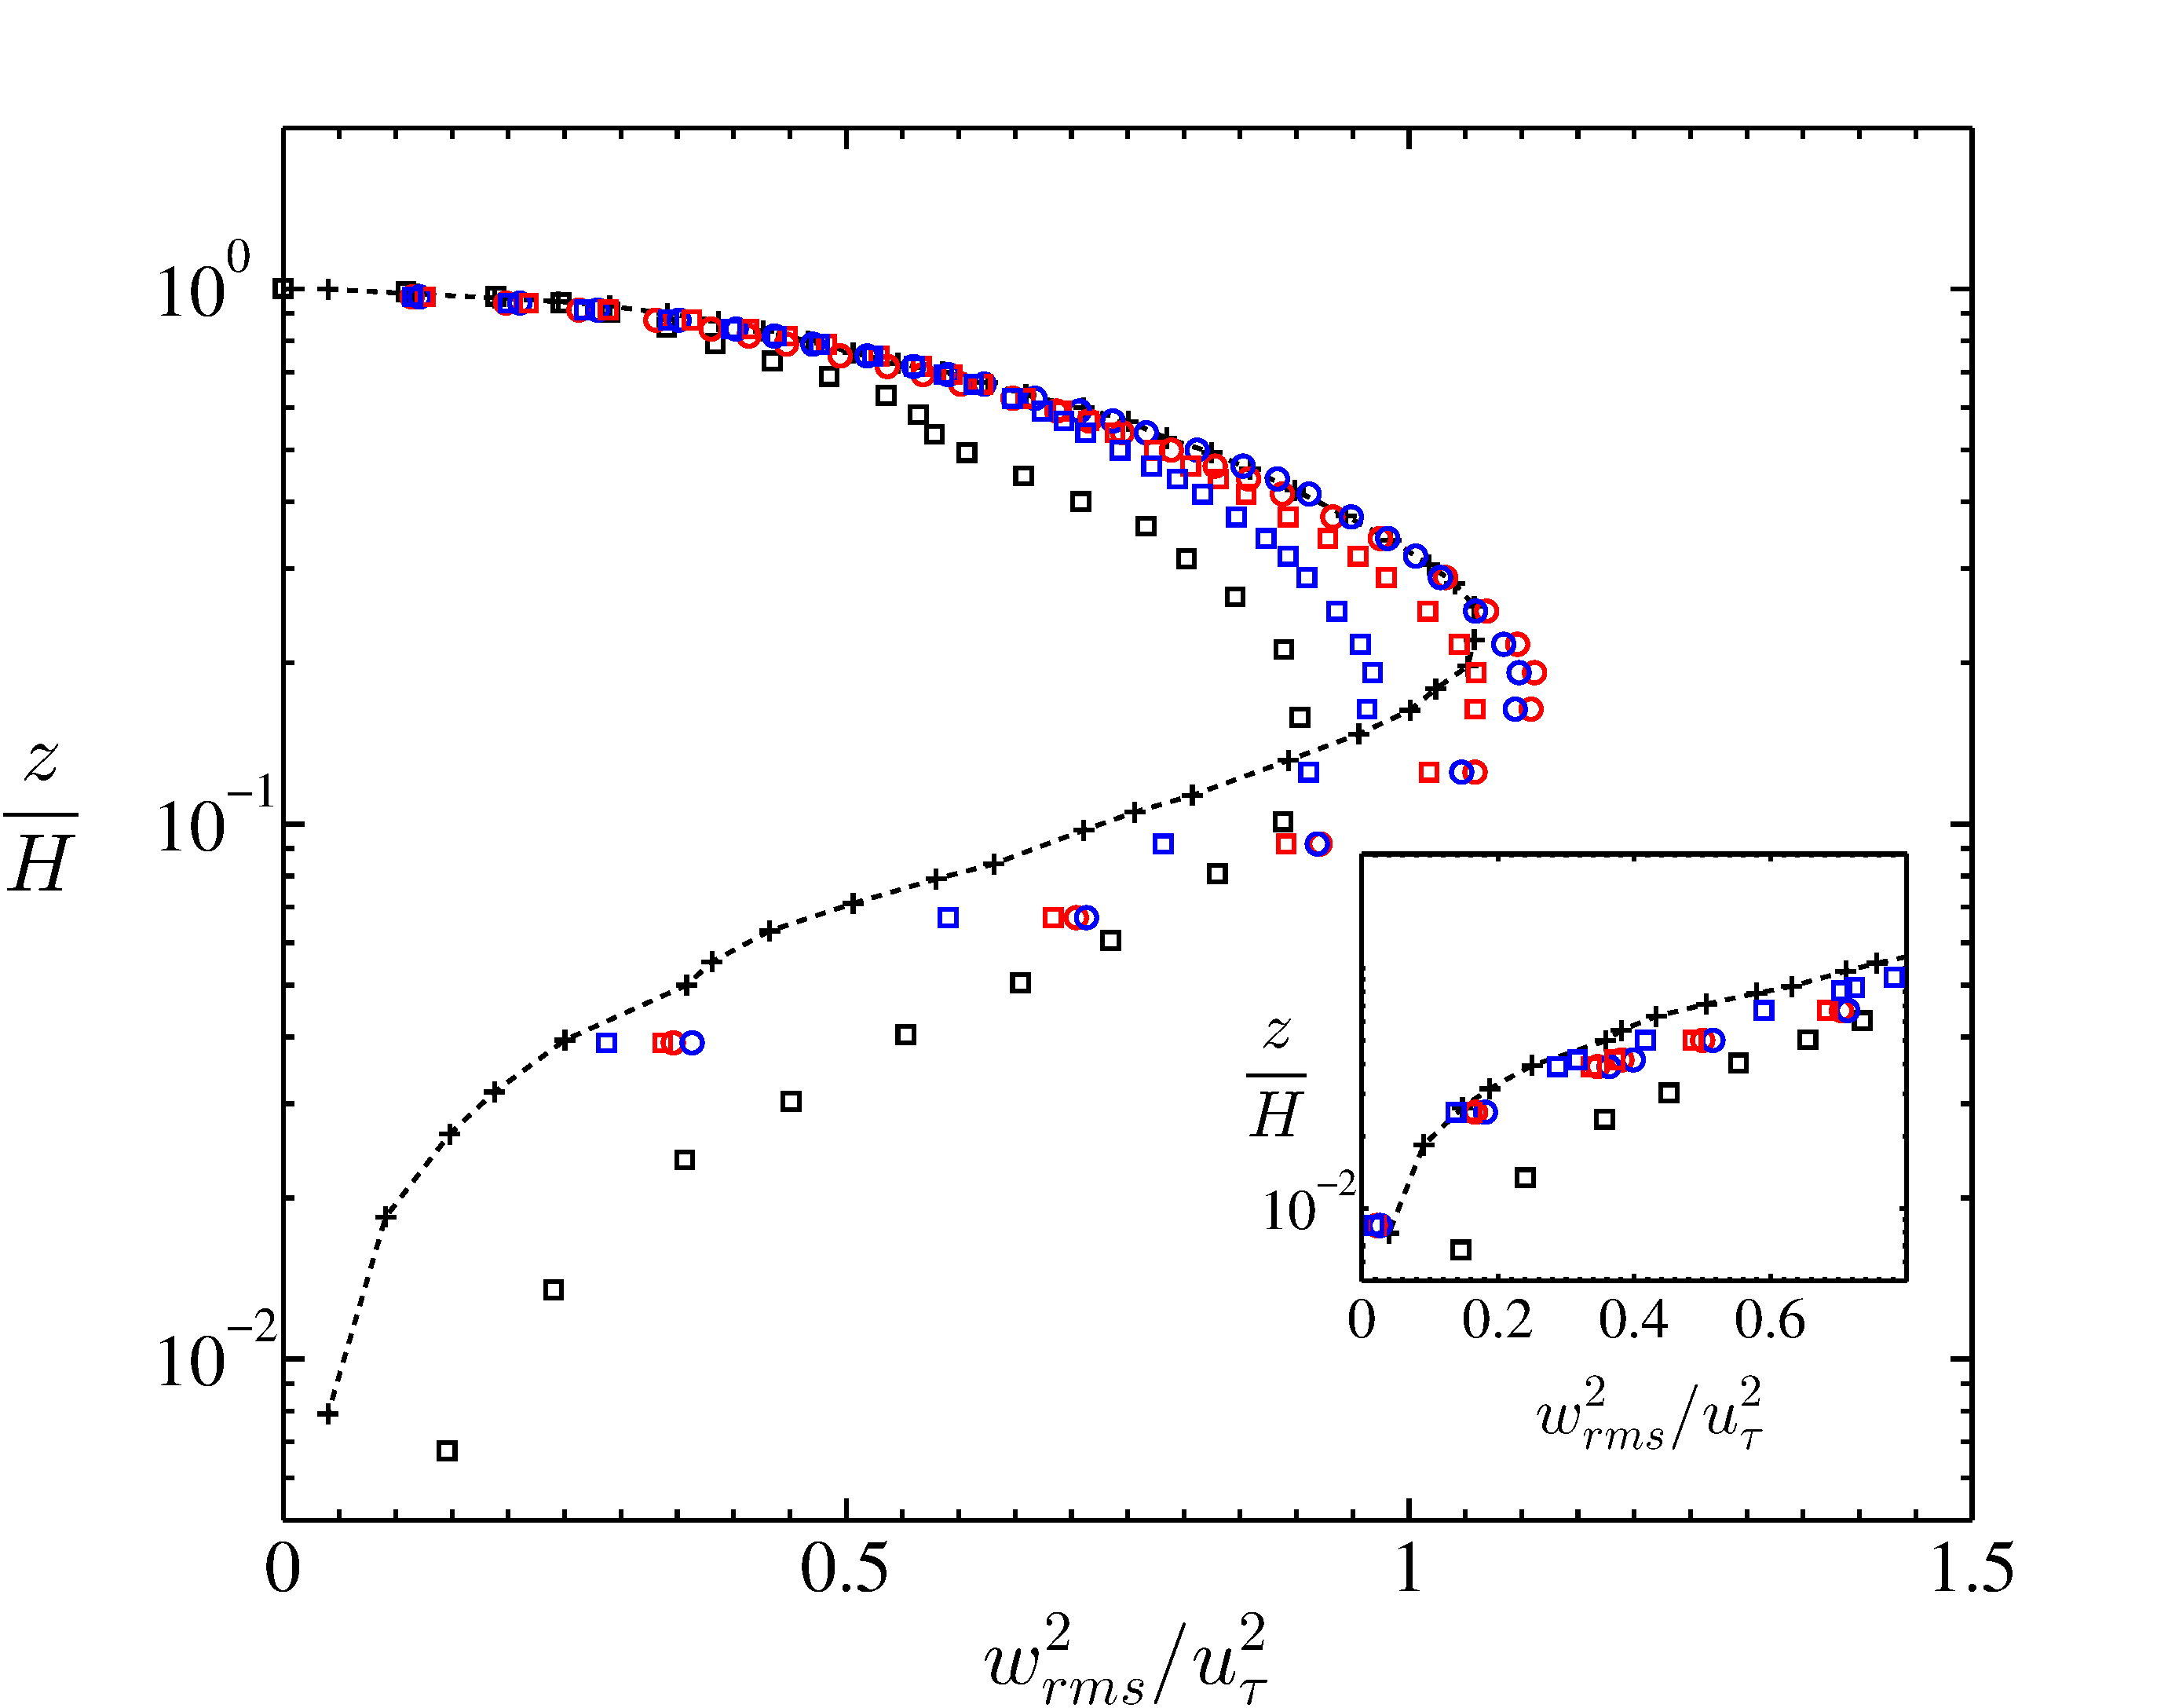
\includegraphics[width=\linewidth]{Fig3/wrms_filter_n2.pdf}
                \caption{}
                \label{fig:wrms}
        \end{subfigure}
        \centering
        \begin{subfigure}[t]{0.75\textwidth}
                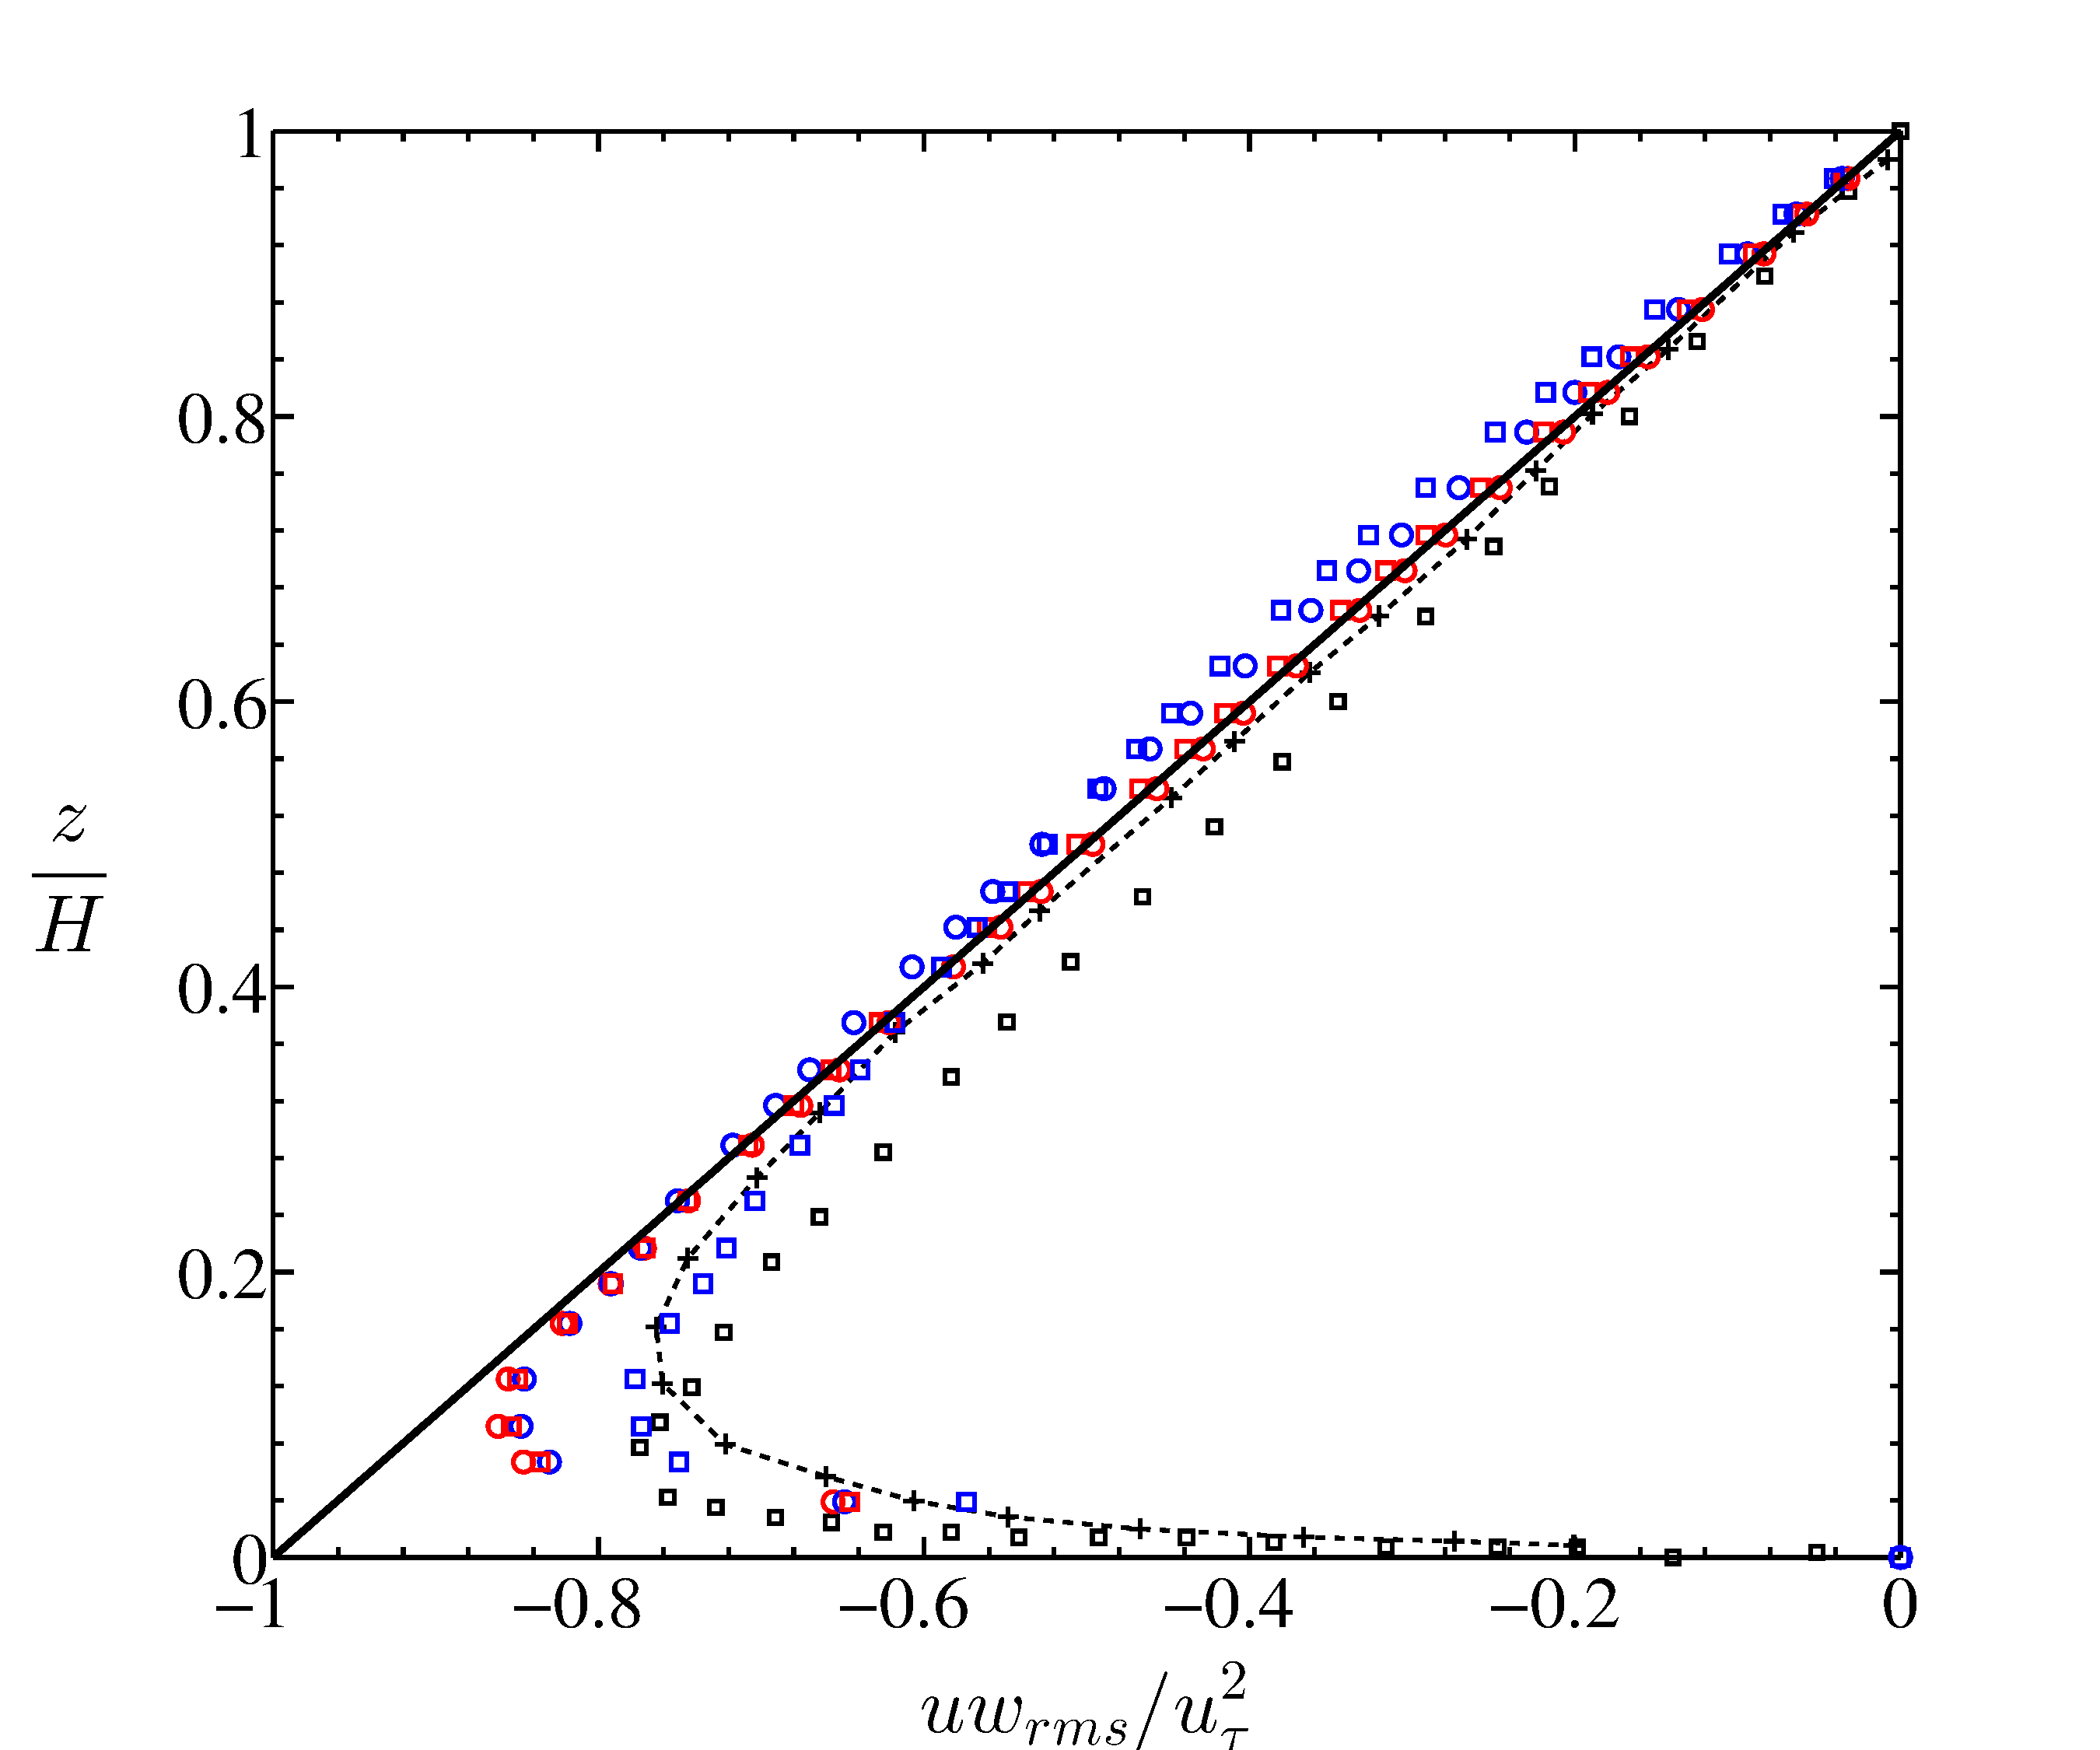
\includegraphics[width=\linewidth]{Fig3/uwrms_filter_n2.pdf}
                \caption{}
                \label{fig:uwrms}
        \end{subfigure}
        \caption[Second order statistics $w_{rms}, \ uw_{rms}$, Case $I-IV$]{Second order statistics for ABL simulations: Case $I-IV$. (a) $w_{rms}$ (b) $uw_{rms}$. Red, Blue curves: current simulations $I-IV$ ($n = 2, \ C_0 = 0.16$);  Red $\Box$, $k_{c}=1$; $\circ$, $k_{c}=2$; Blue $\circ$, $k_{c} = 4$; Blue $\Box$, $k_{c} = 6$.  Black $-+$, standard Smagorinsky ($C_s = 0.10, n = 2$) and black $\Box$ scale dependant dynamic Smagorinsky for Port$\acute{e}$-Agel et al.~\cite{porte1fun}. Solid black line in (b) is the ideal linear trend of non-dimensional total stress.}\label{fig:stat22}
\end{figure}
\subsection{Cases V-VII}
This section describes the statistics involved with tuning parameters $C_0 = 0.17, n = 1$.  The non-dimensional velocity gradient in Figure~\ref{fig:statba} shows similar trends with Chow et. al~\cite{chow} as was observed in Cases I-IV. The log-layer mismatch with $k_c = 2$ is slightly higher ($\sim 60\%$) compared to the mismatch with $k_c = 4, 6$ ($\sim 40-50\%$) and the peak is closer towards the wall compared to the cases I-IV. The plot with $k_c = 6$ shows some reminiscent logarithmic trends {in the first $15-20\%$} of the ABL and yet displays some prominence in the wake region ($\phi(z) > 1$), compared to $k_c = 2, 4$. All the plots with different $k_c$ show a relatively slower decay to the ``flat-profile" region compared to the plots with $n=2$ (Cases I - IV).\\
The results of second order statistics are shown in Figure{s}~\ref{fig:stat021a},~\ref{fig:stat022a}. The plots with $k_c = 4, 6$ show excellent match with the standard Smagorinsky model in the outer layer of the flow~\cite{porte1fun}. The discrepancies in the inner layer compared to the Cases I-IV can be manifested in the 
{smaller values}  of resolved ``stresses" (especially $v_{rms}$, $w_{rms}$, $uw_{rms}$) with $k_c = 4$ instead of $k_c = 6$ as observed in Cases I-IV. To summarize, 
%even 
with $n = 1, C_0 = 0.17$, the phenomenon of ``logarithmic mismatch" can {still} be seen as in Case I-IV. 
\begin{figure}
\centering
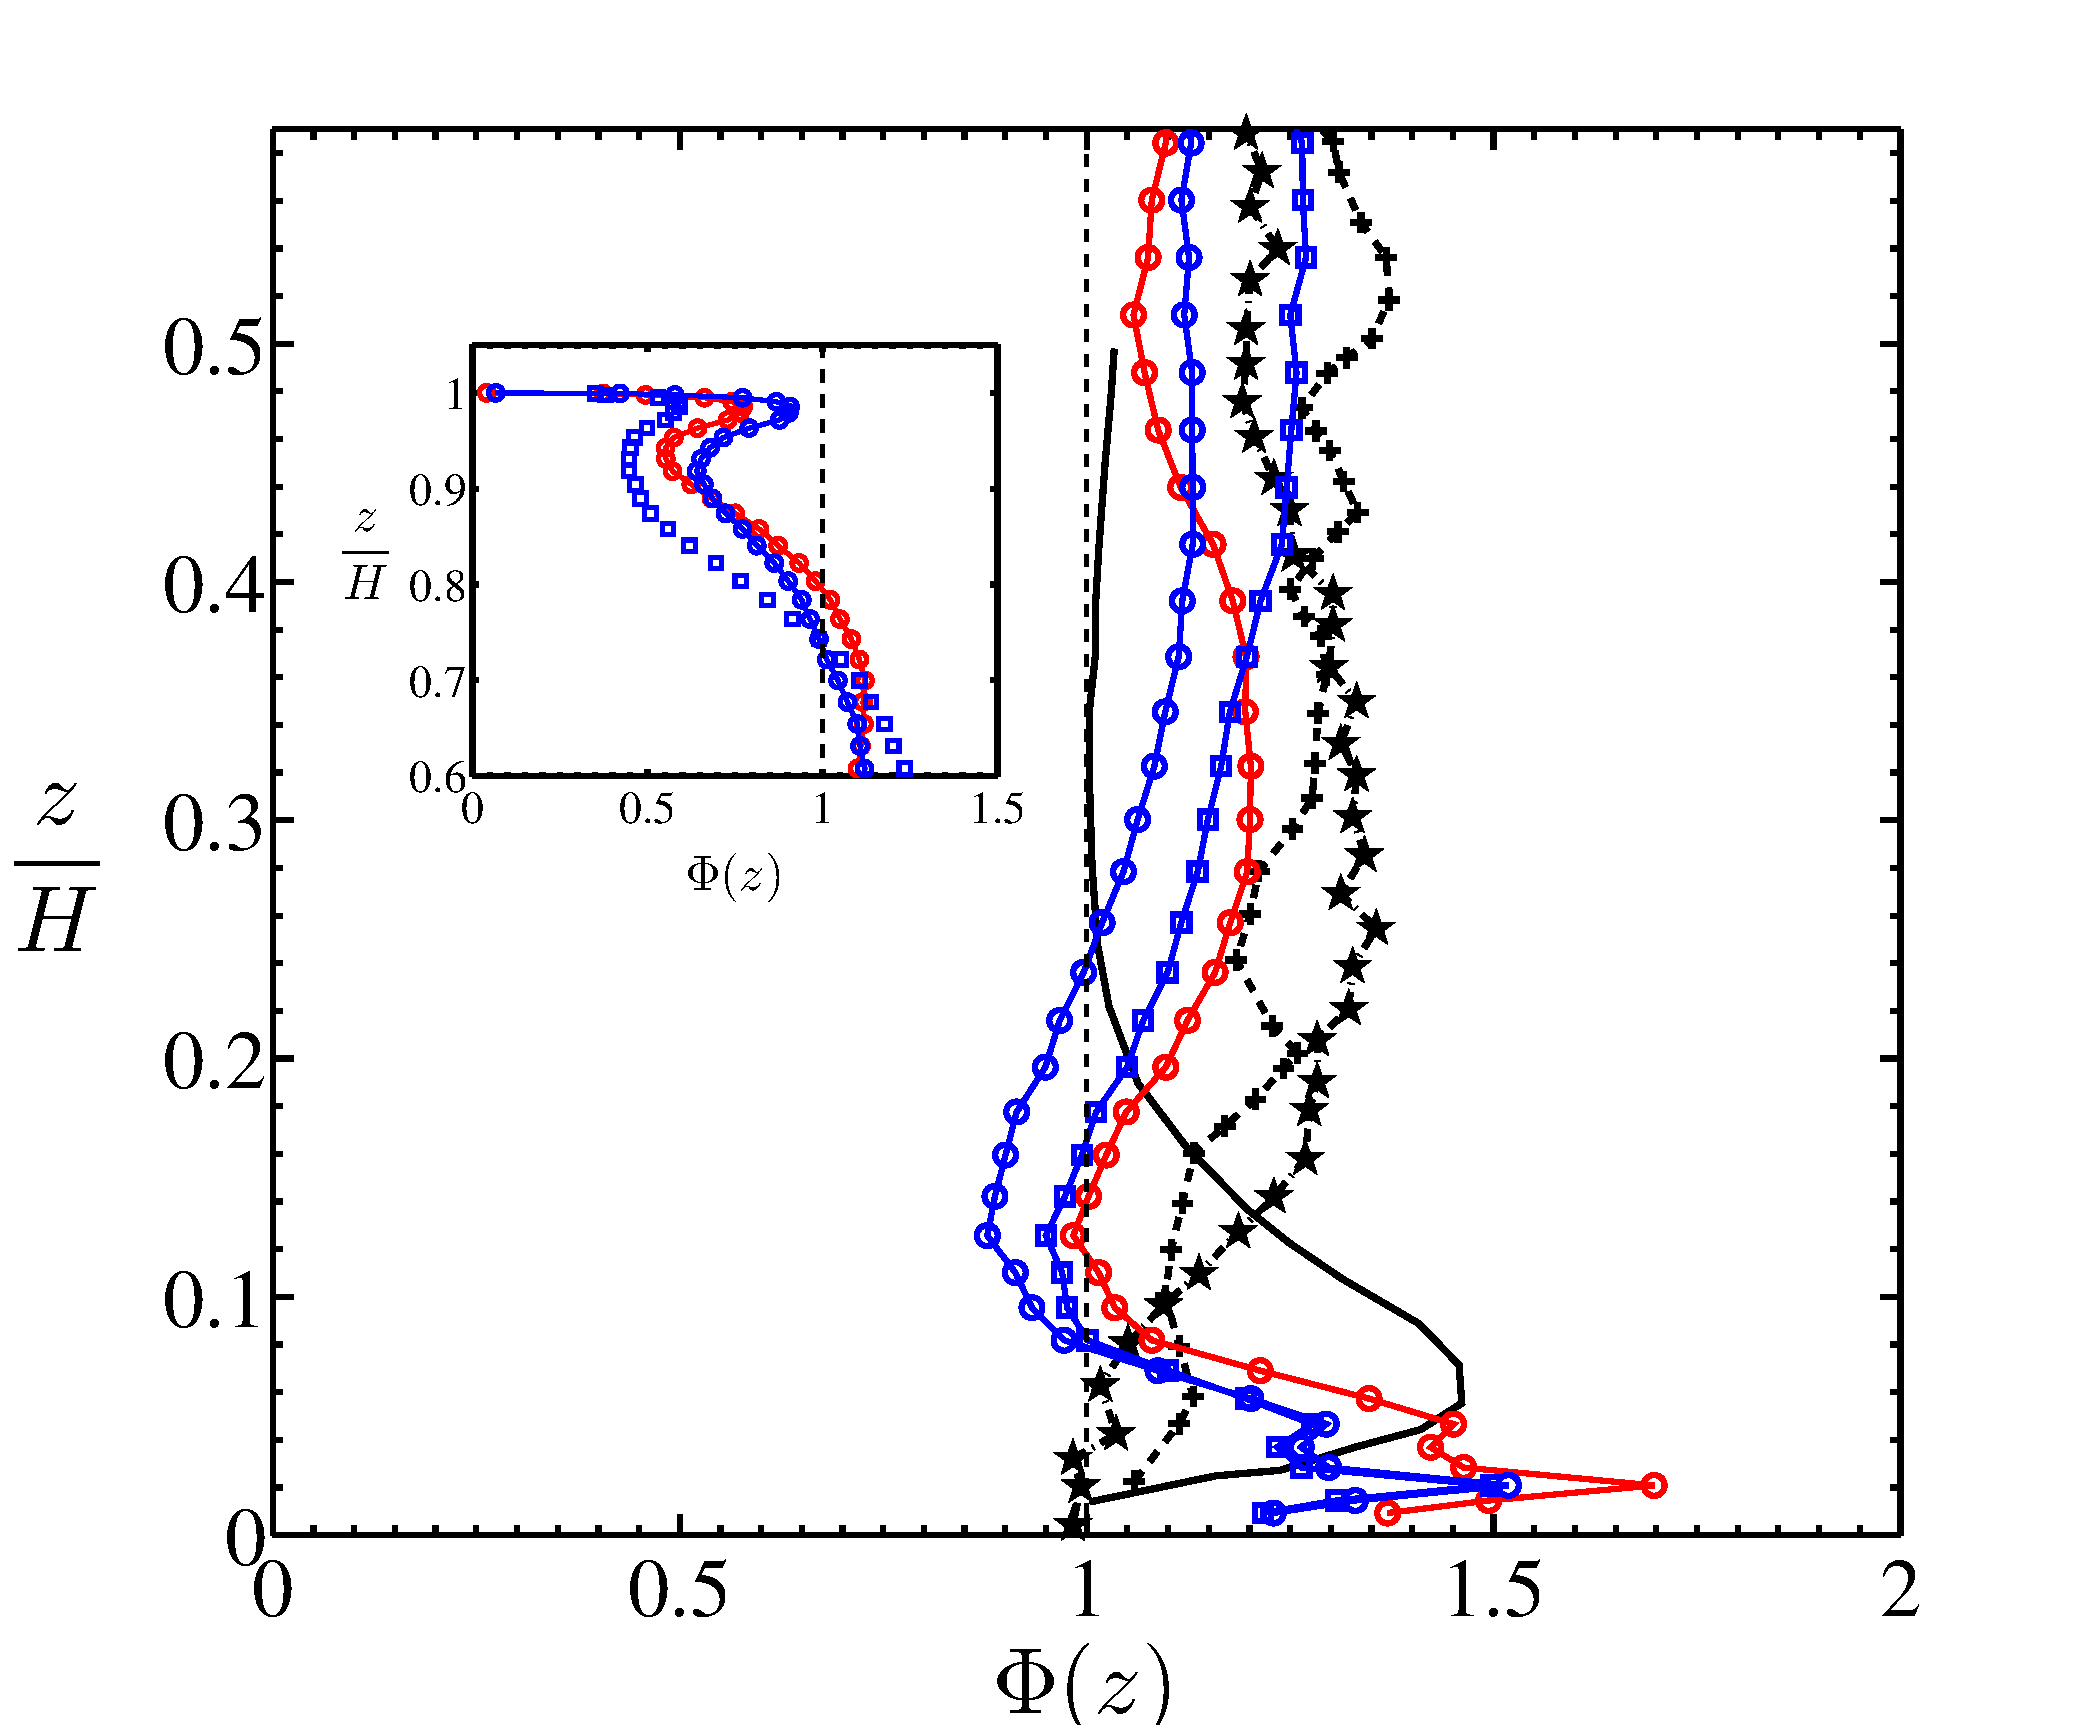
\includegraphics[width = 0.75\linewidth]{Fig3/gradient_filt_n1.pdf}        
        \caption[$\Phi(z)$, Case $V-VII$]{Non dimensinonal mean streamwise velocity gradient $\phi(z)$ vs $z/H$. Red, Blue curves: current simulations $V-VII$ ($n = 1, \ C_0 = 0.17$); Black curves from the literature~\cite{porte1fun,bou1}. Red $\circ$, $k_{c}=2$; Blue $\circ$, $k_{c} = 4$; Blue $\Box$, $k_{c} = 6$. Black $+$ scale dependant dynamic Smagorinsky for Port$\acute{e}$-Agel et al.~\cite{porte1fun}; $-$ , standard Smagorinsky, $\star$, Lagrangian scale dependant dynamic Smagorinsky with filtering, Bou-Zeid et. al~\cite{bou1}}\label{fig:statba}
\end{figure}

\begin{figure}
\centering
        \begin{subfigure}[t]{0.75\textwidth}
                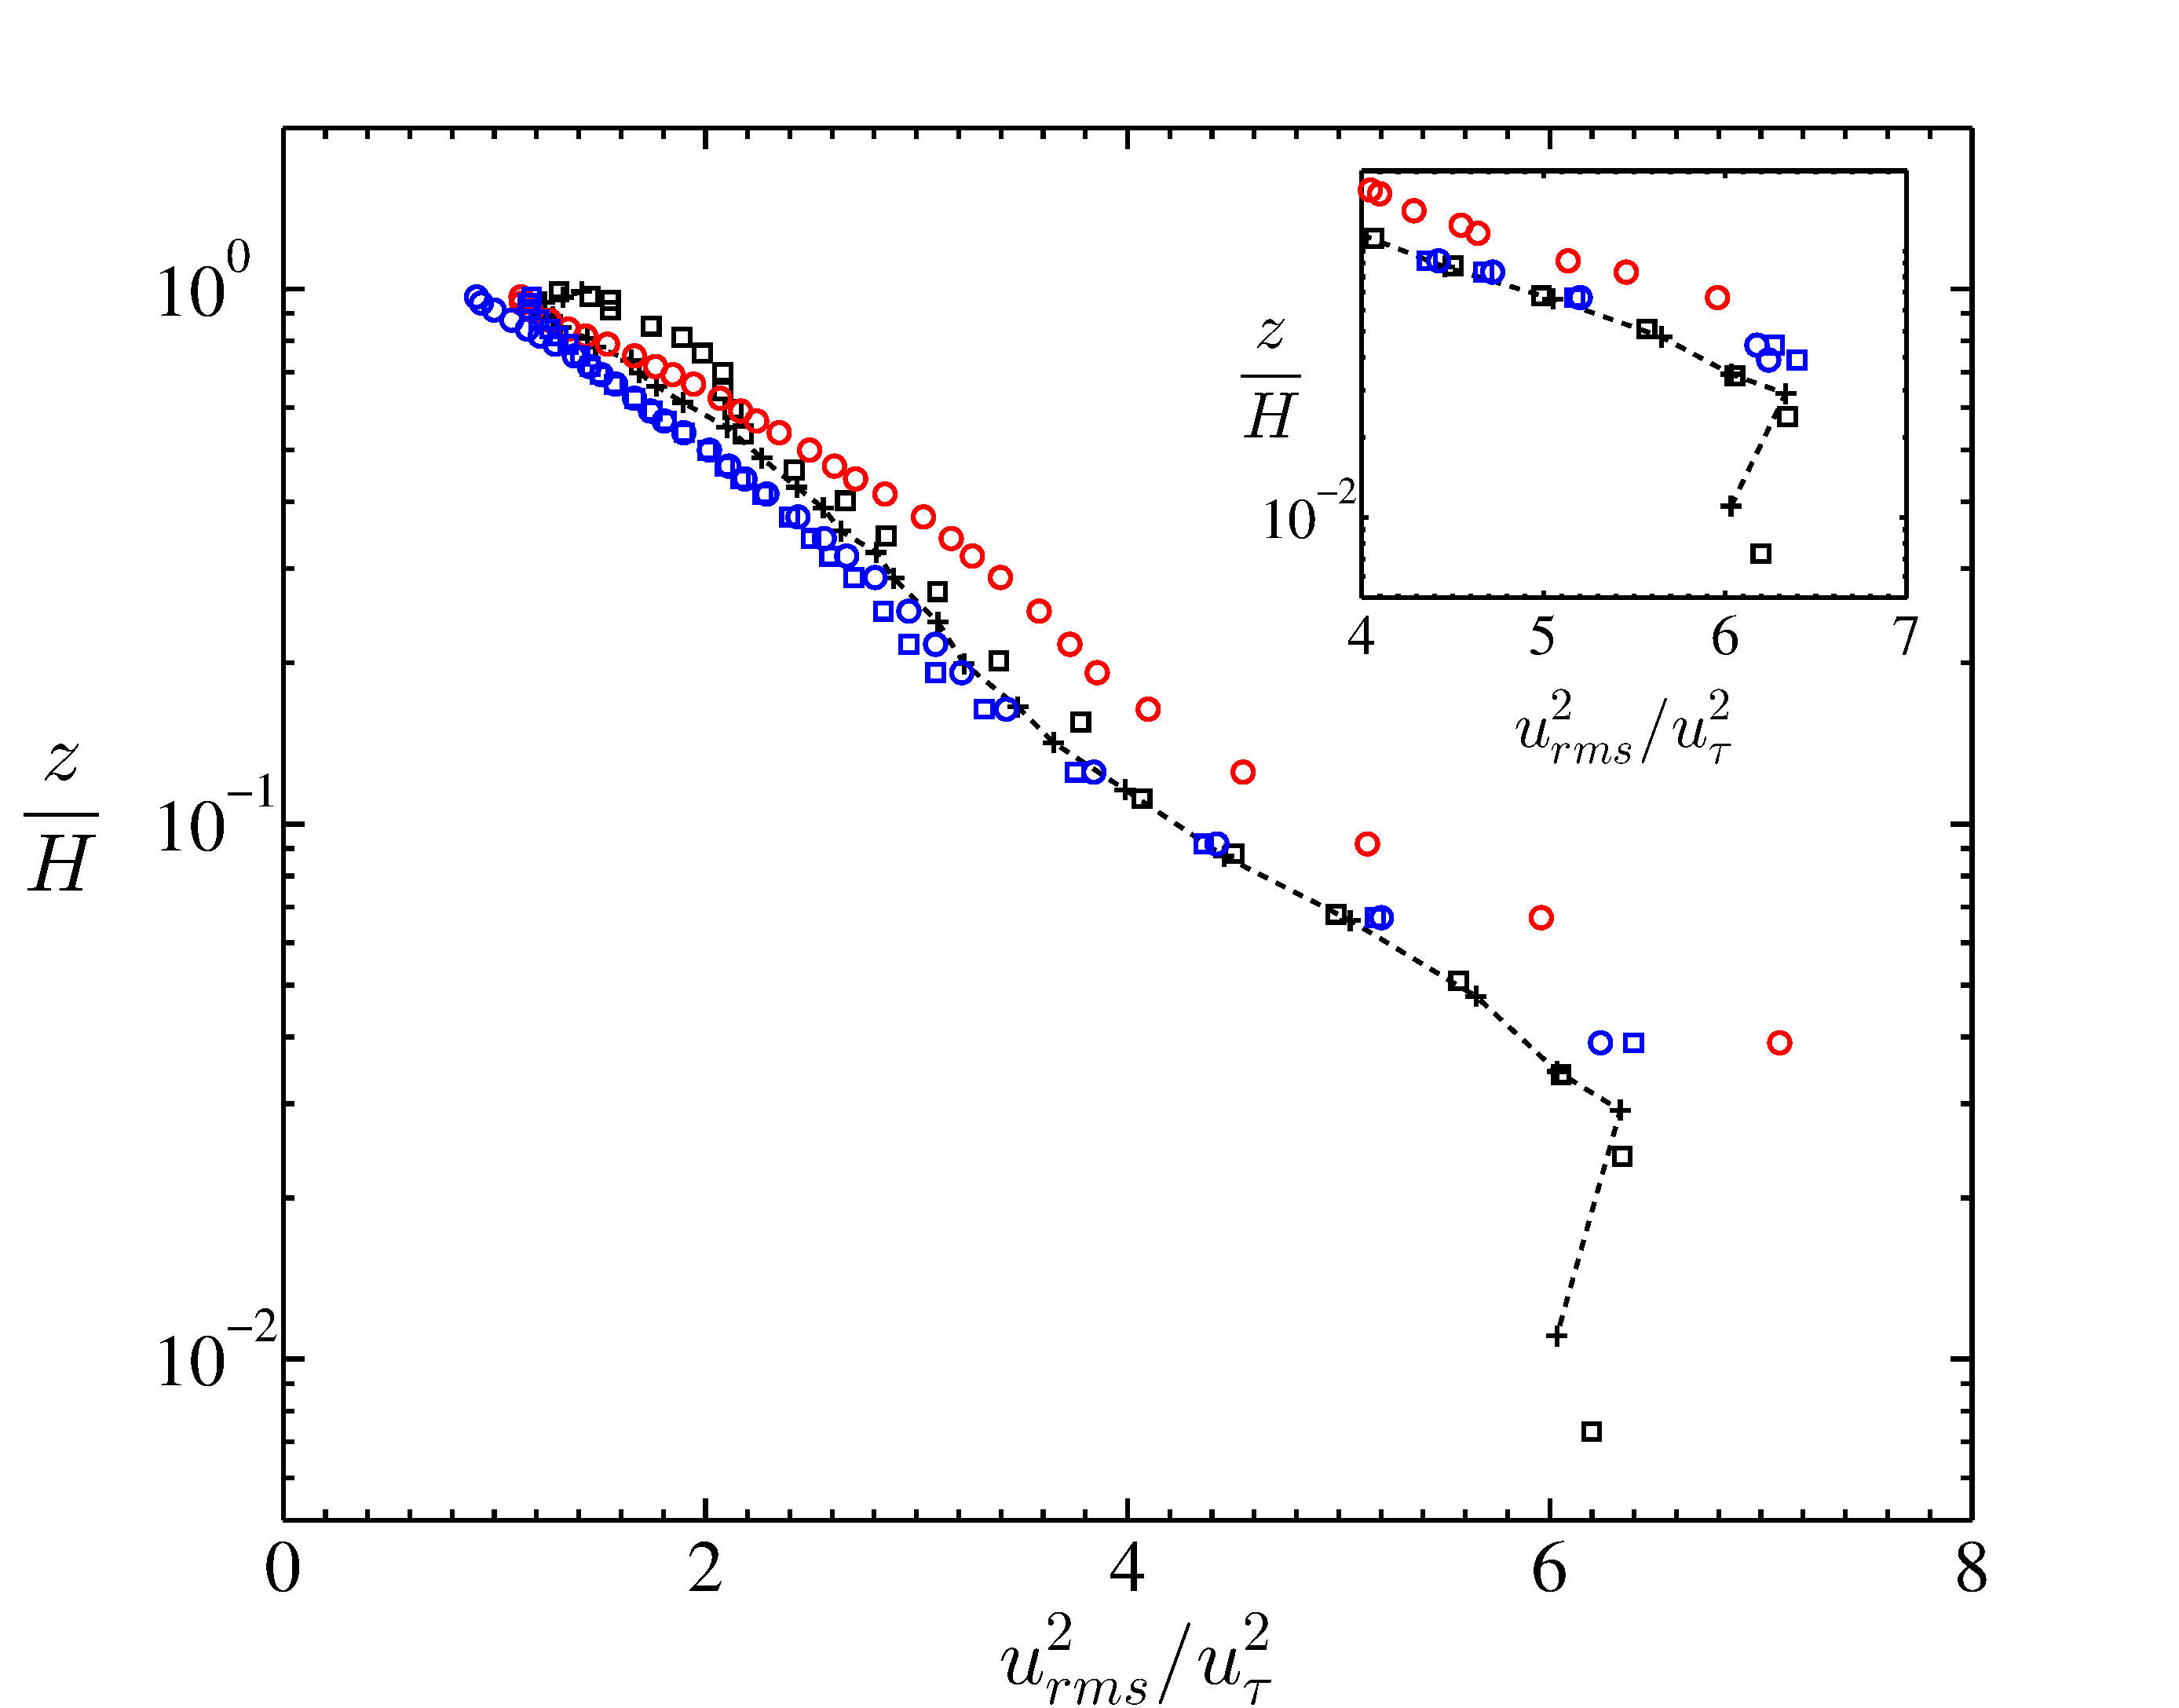
\includegraphics[width=\linewidth]{Fig3/urms_filter_n1.pdf}
                \caption{}
                \label{fig:urms1a}
        \end{subfigure}
        \centering
        \begin{subfigure}[t]{0.75\textwidth}
                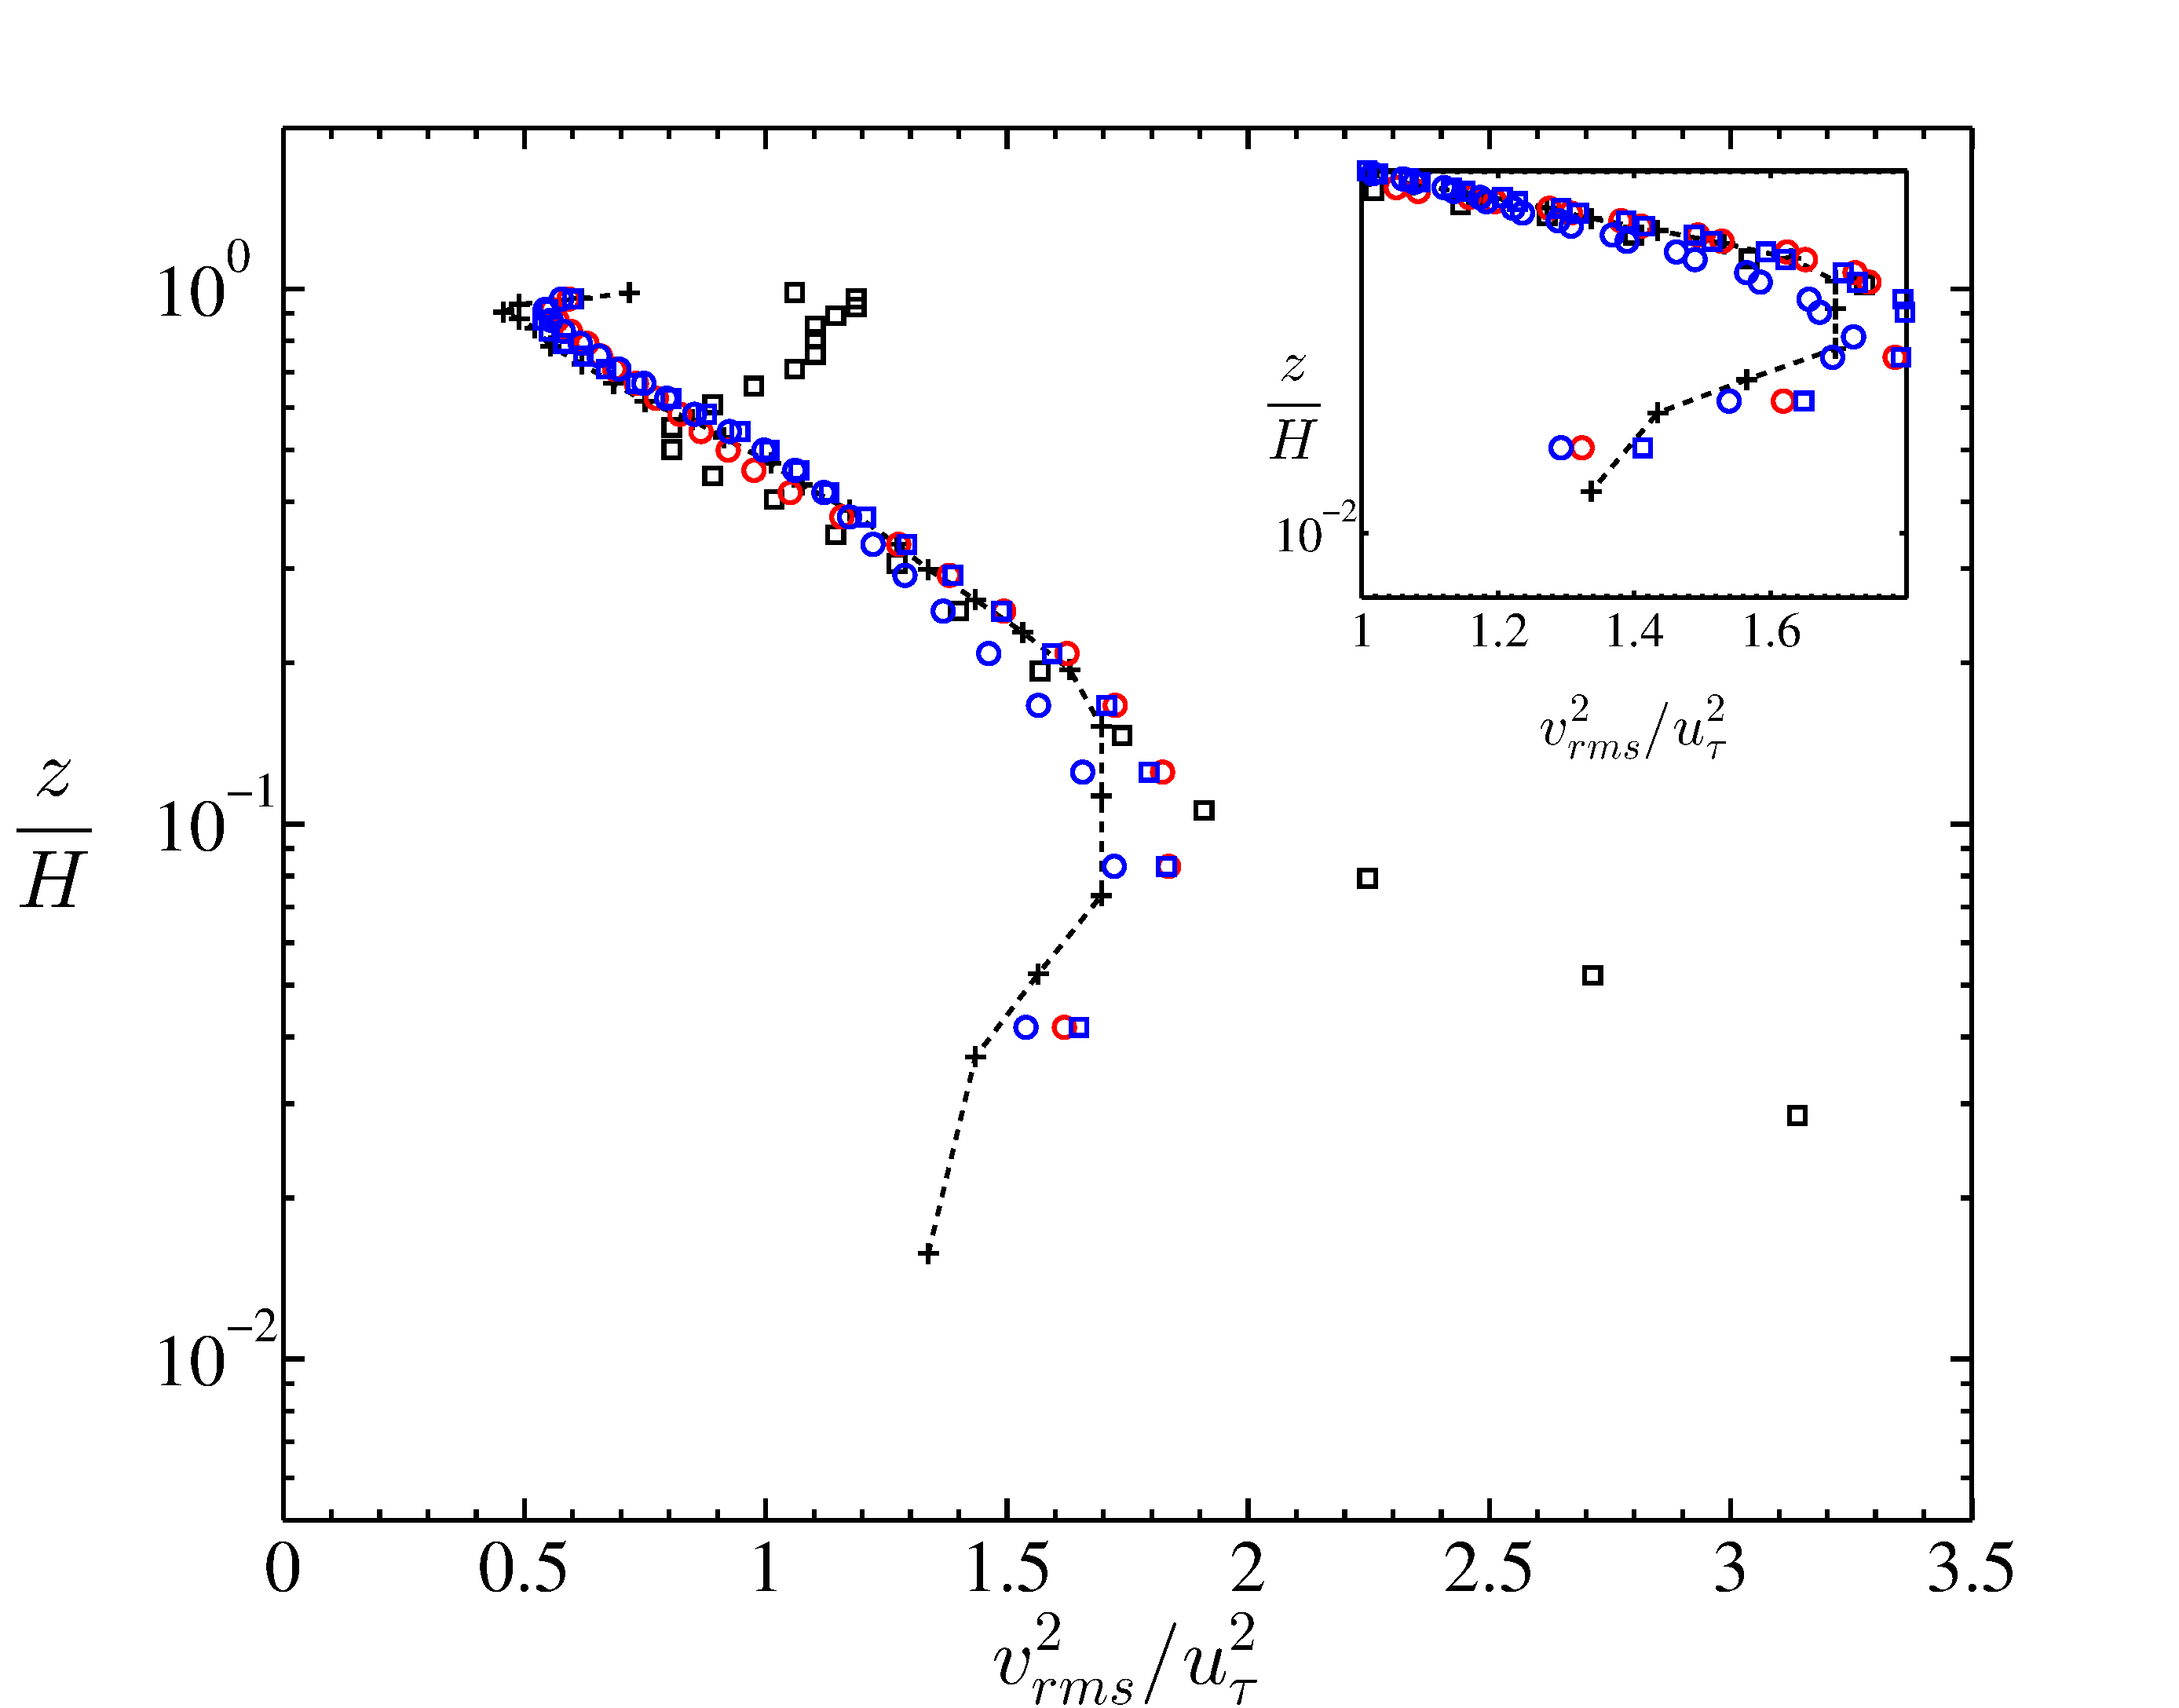
\includegraphics[width=\linewidth]{Fig3/vrms_filter_n1.pdf}
                \caption{}
                \label{fig:vrms1a}
        \end{subfigure}
        \caption[Second order statistics $u_{rms}, \ v_{rms}$, Case $V-VII$]{Second order statistics for ABL simulations: Case $V-VII$ . (a) $u_{rms}$ (b) $v_{rms}$ . Red, Blue curves: current simulations $V-VII$ ($n = 1, \ C_0 = 0.17$);  Red $\circ$, $k_{c}=2$; Blue $\circ$, $k_{c} = 4$; Blue $\Box$, $k_{c} = 6$.  Black $-+$, standard Smagorinsky ($C_s = 0.10, n = 2$) {for Port$\acute{e}$-Agel et al.~\cite{porte1fun}} and black $\Box$ scale dependant dynamic Smagorinsky for Port$\acute{e}$-Agel et al.~\cite{porte1fun}. }\label{fig:stat021a}
\end{figure}
\begin{figure}
        \centering
        \begin{subfigure}[t]{0.75\textwidth}
                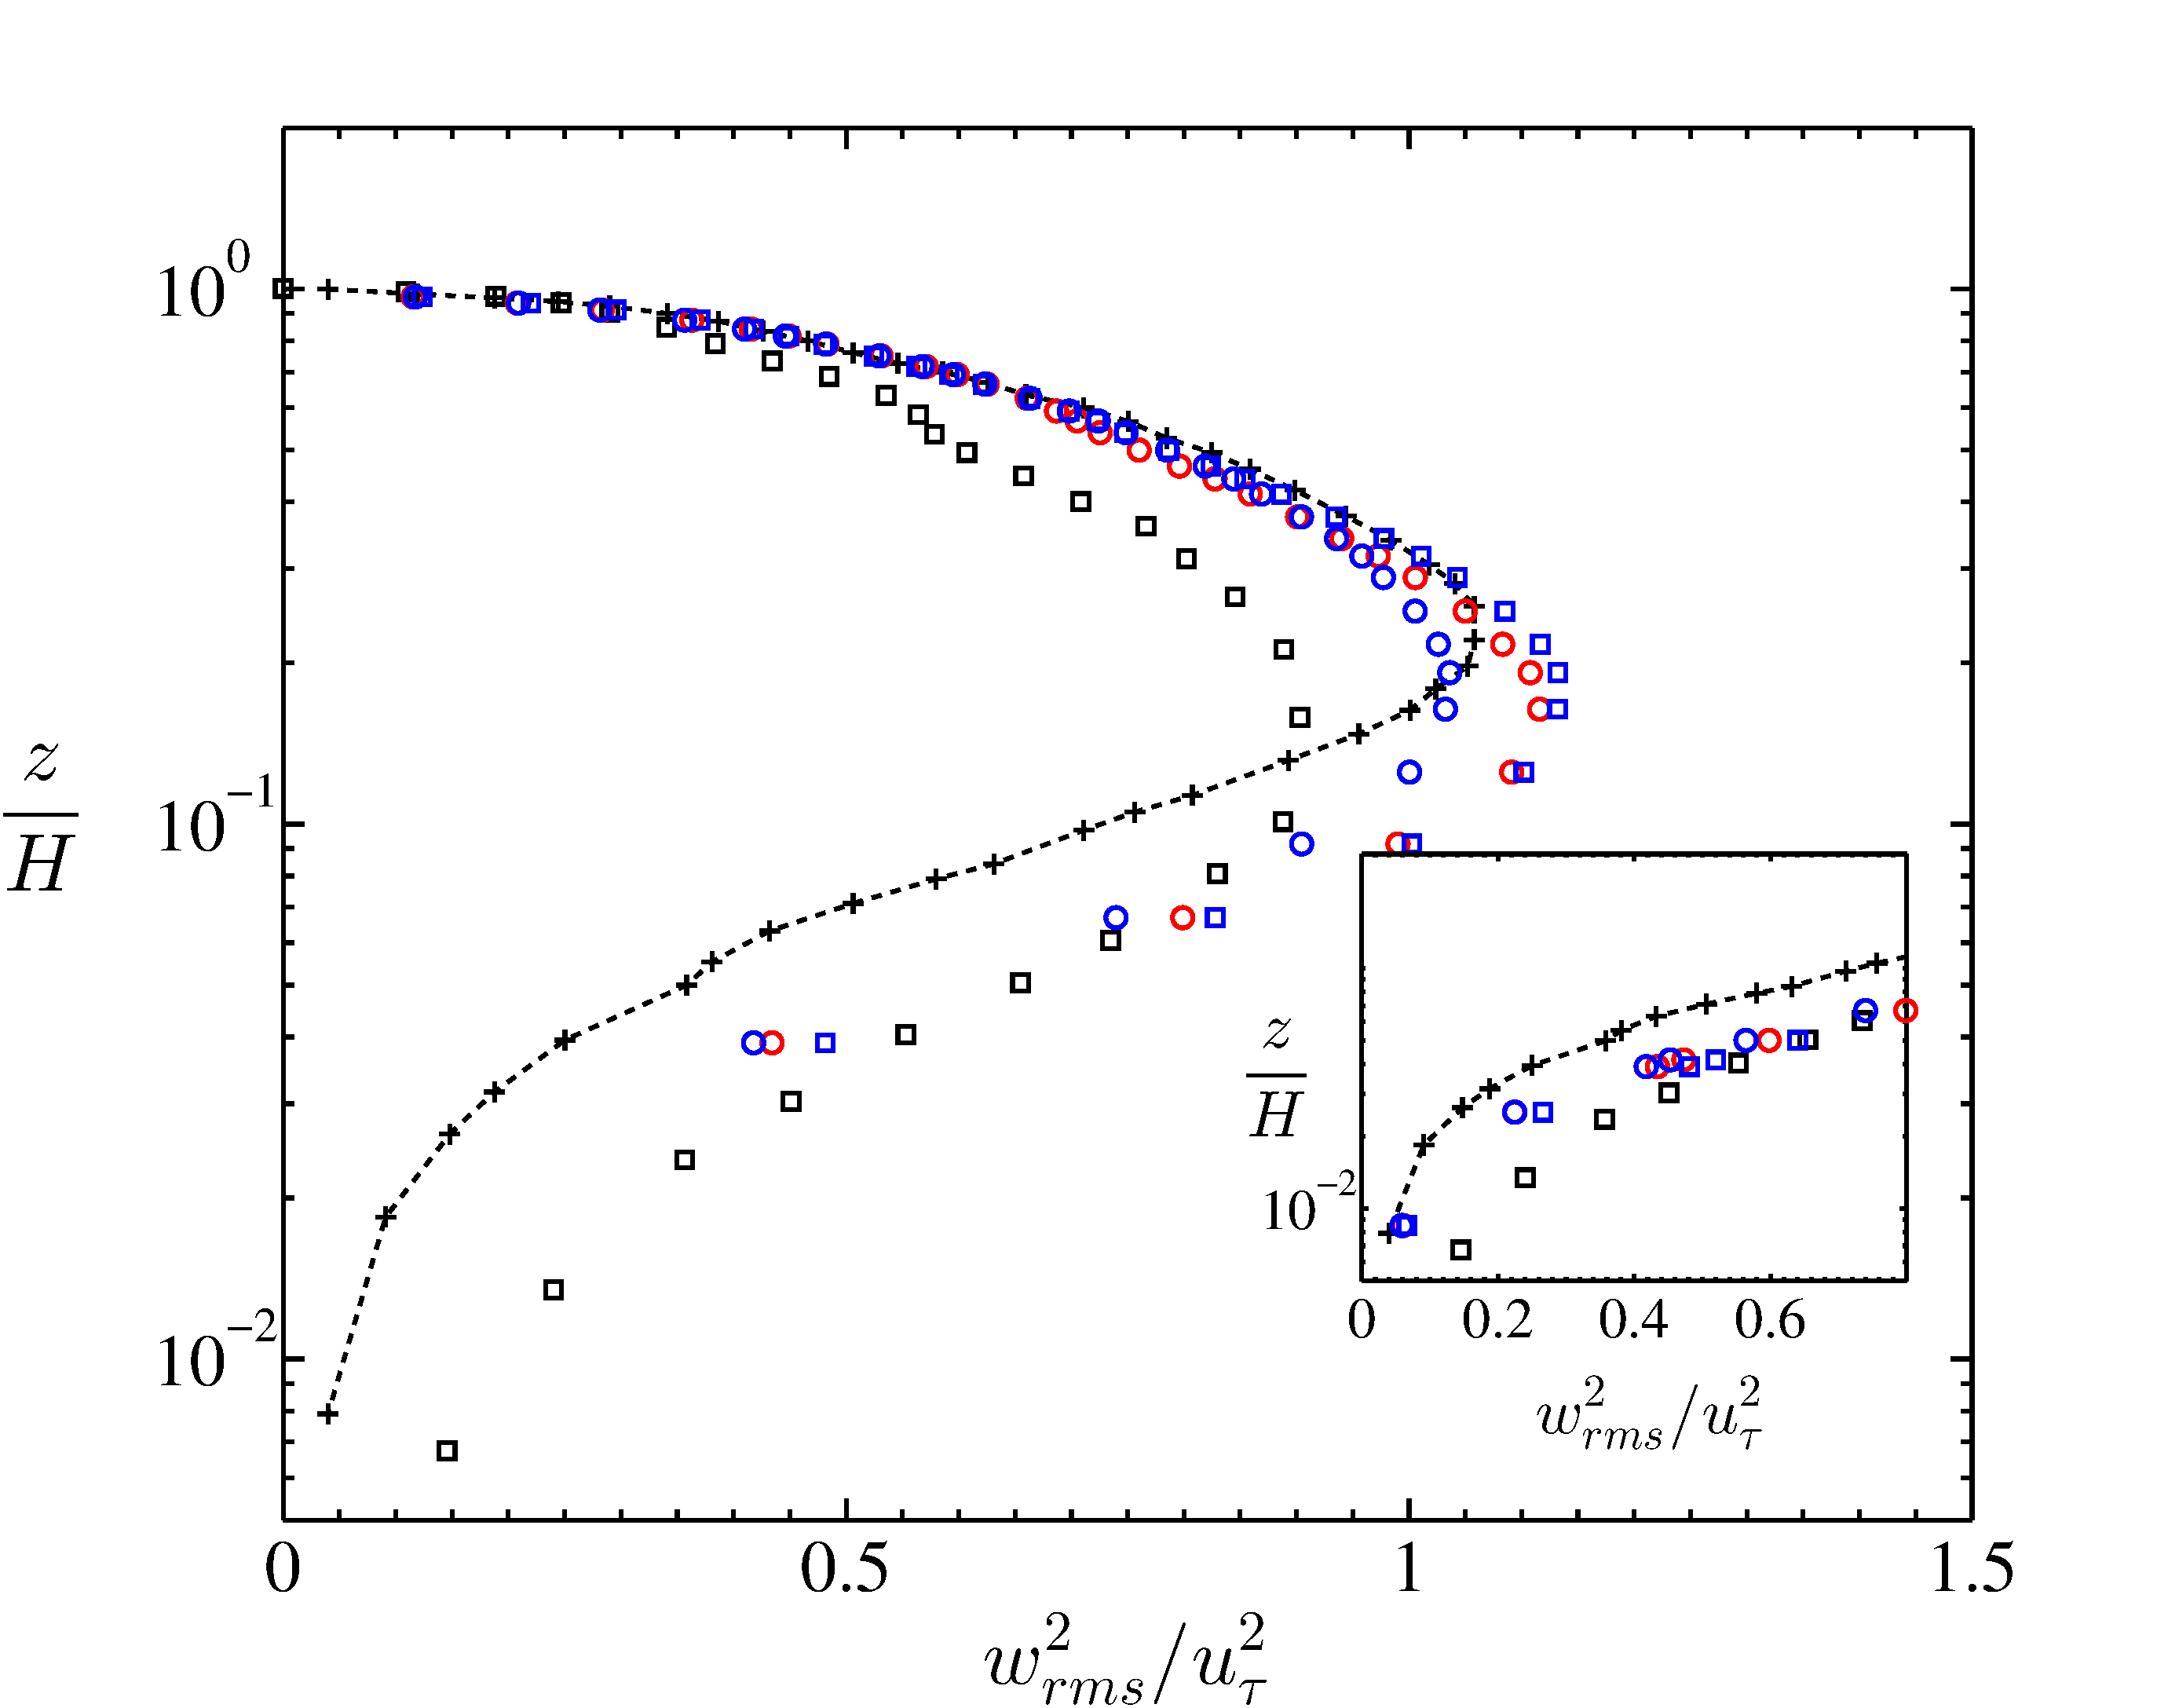
\includegraphics[width=\linewidth]{Fig3/wrms_filter_n1.pdf}
                \caption{}
                \label{fig:wrms1a}
        \end{subfigure}
        \centering
        \begin{subfigure}[t]{0.75\textwidth}
                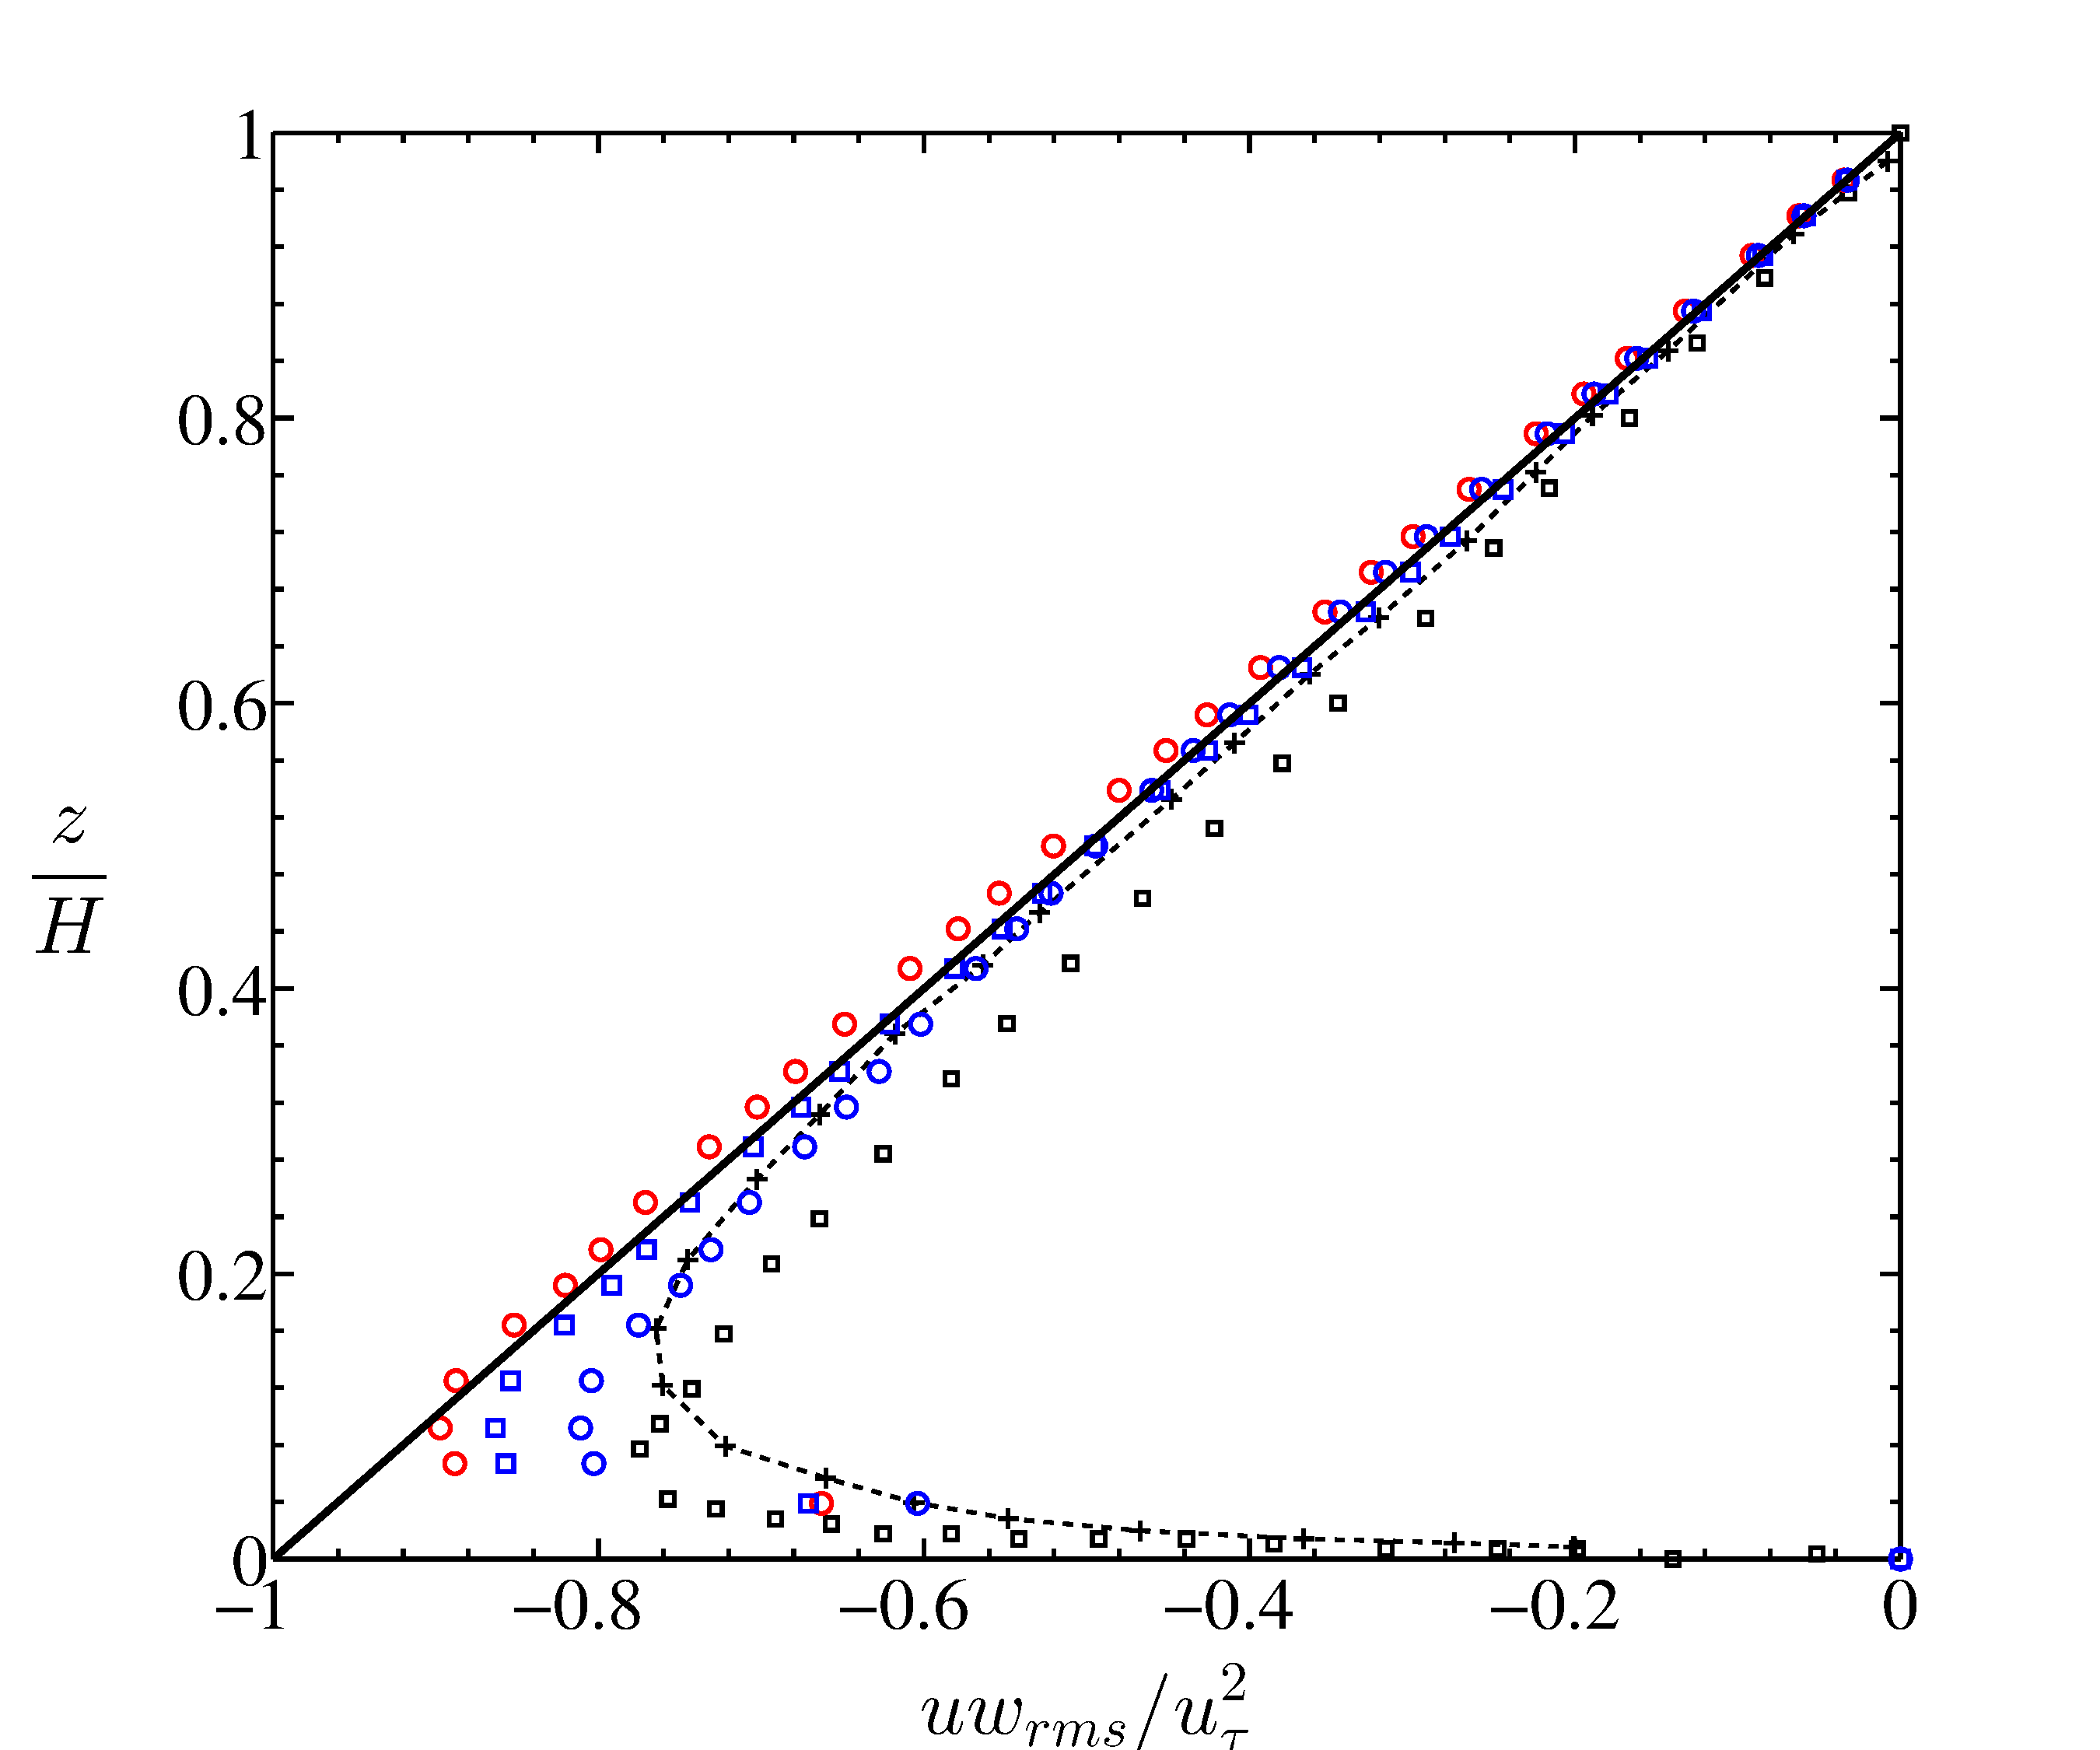
\includegraphics[width=\linewidth]{Fig3/uwrms_filter_n1.pdf}
                \caption{}
                \label{fig:uwrms1a}
        \end{subfigure}%
        \caption[Second order statistics $w_{rms}, \ uw_{rms}$, Case $V-VII$]{Second order statistics for ABL simulations: Case $V-VII$ . (a) $w_{rms}$ (b) $uw_{rms}$ . Red, Blue curves: current simulations $V-VII$ ($n = 1, \ C_0 = 0.17$);  Red $\circ$, $k_{c}=2$; Blue $\circ$, $k_{c} = 4$; Blue $\Box$, $k_{c} = 6$.  Black $-+$, standard Smagorinsky ($C_s = 0.10, n = 2$)  {for Port$\acute{e}$-Agel et al.~\cite{porte1fun}} and black $\Box$ scale dependant dynamic Smagorinsky for Port$\acute{e}$-Agel et al.~\cite{porte1fun}. Solid black line in (b) is the ideal linear trend of non-dimensional total stress. }\label{fig:stat022a}
\end{figure}

\subsection{Cases VIII-X}
With the tuning parameters $C_0 = 0.19, n = 0.5$, the law of the wall shows significant improvements in the near wall region as depicted in Figure~\ref{fig:statb} with the maximum log-law deviation suppressed to 5\% in the lower $10\%$ of ABL. The results are found to be quite comparable with the scale-dependant models of Porte-Ag\'{e}l et. al~\cite{porte1fun} and Bou-Zeid et. al~\cite{bou1} especially with $k_c = 4$. Specifically, {our} results at {$z/H\preceq 0.1$} 
%are exactly intermediate 
{lie in the middle}
between planar averaged scale dependant model of Porte-Ag\'{e}l and its superior Lagrangian averaging counterpart~\cite{bou1}. The plots of $k_c = 2,4,6$ are {practically} indifferent in the near wall region $z/H \sim 0.05-0.1$, beyond which significant differences are registered. For higher explicit filtering with $k_c = 6$, there is a slight negative value of the gradient $\Phi$ at $z/H \sim 0.01$ even though the error is still within $10\%$. The filtering results do not show {significant conspicuousness} in the ``wake-region" except for $k_c = 4$. (The wake region starts at $z/H \sim 0.3-0.4$, when $\Phi(z) > 1$ ). The mean velocity profile gradually decays to {flat profile} with zero gradient as it approaches the top symmetry boundary conditions.{It is observed that in Cases VIII-X, the decay from wake profile to flat profile occurs quite quickly as opposed to a relatively suppressed decay in Cases I-IV.} 
The second order statistics are shown in Figure~\ref{fig:stat021},~\ref{fig:stat022}. The results shows reasonable similarity and sometimes over-prediction of the resolved Reynolds stresses compared to the dynamic Smagorinsky model. {It is quite intriguing to note that a simple change of the shape function of the Smagorinsky mixing length (increasing $dC_s/dz$) has profound impact on the near wall stresses, especially, $u_{rms}, v_{rms}$ which instead of decaying to zero at `` {wall} " for Cases I-IV, actually show a peak at the approximate `` \textit{wall} " similar to the trends of standard dynamic models.}  The results with $k_c=6$ show similar effects of diffusion and {under-prediction of peaks as in case $I-IV$ compared to other values of $k_c$,}  even though the underprediction is much more benign than the previous cases.

\begin{figure}
\centering
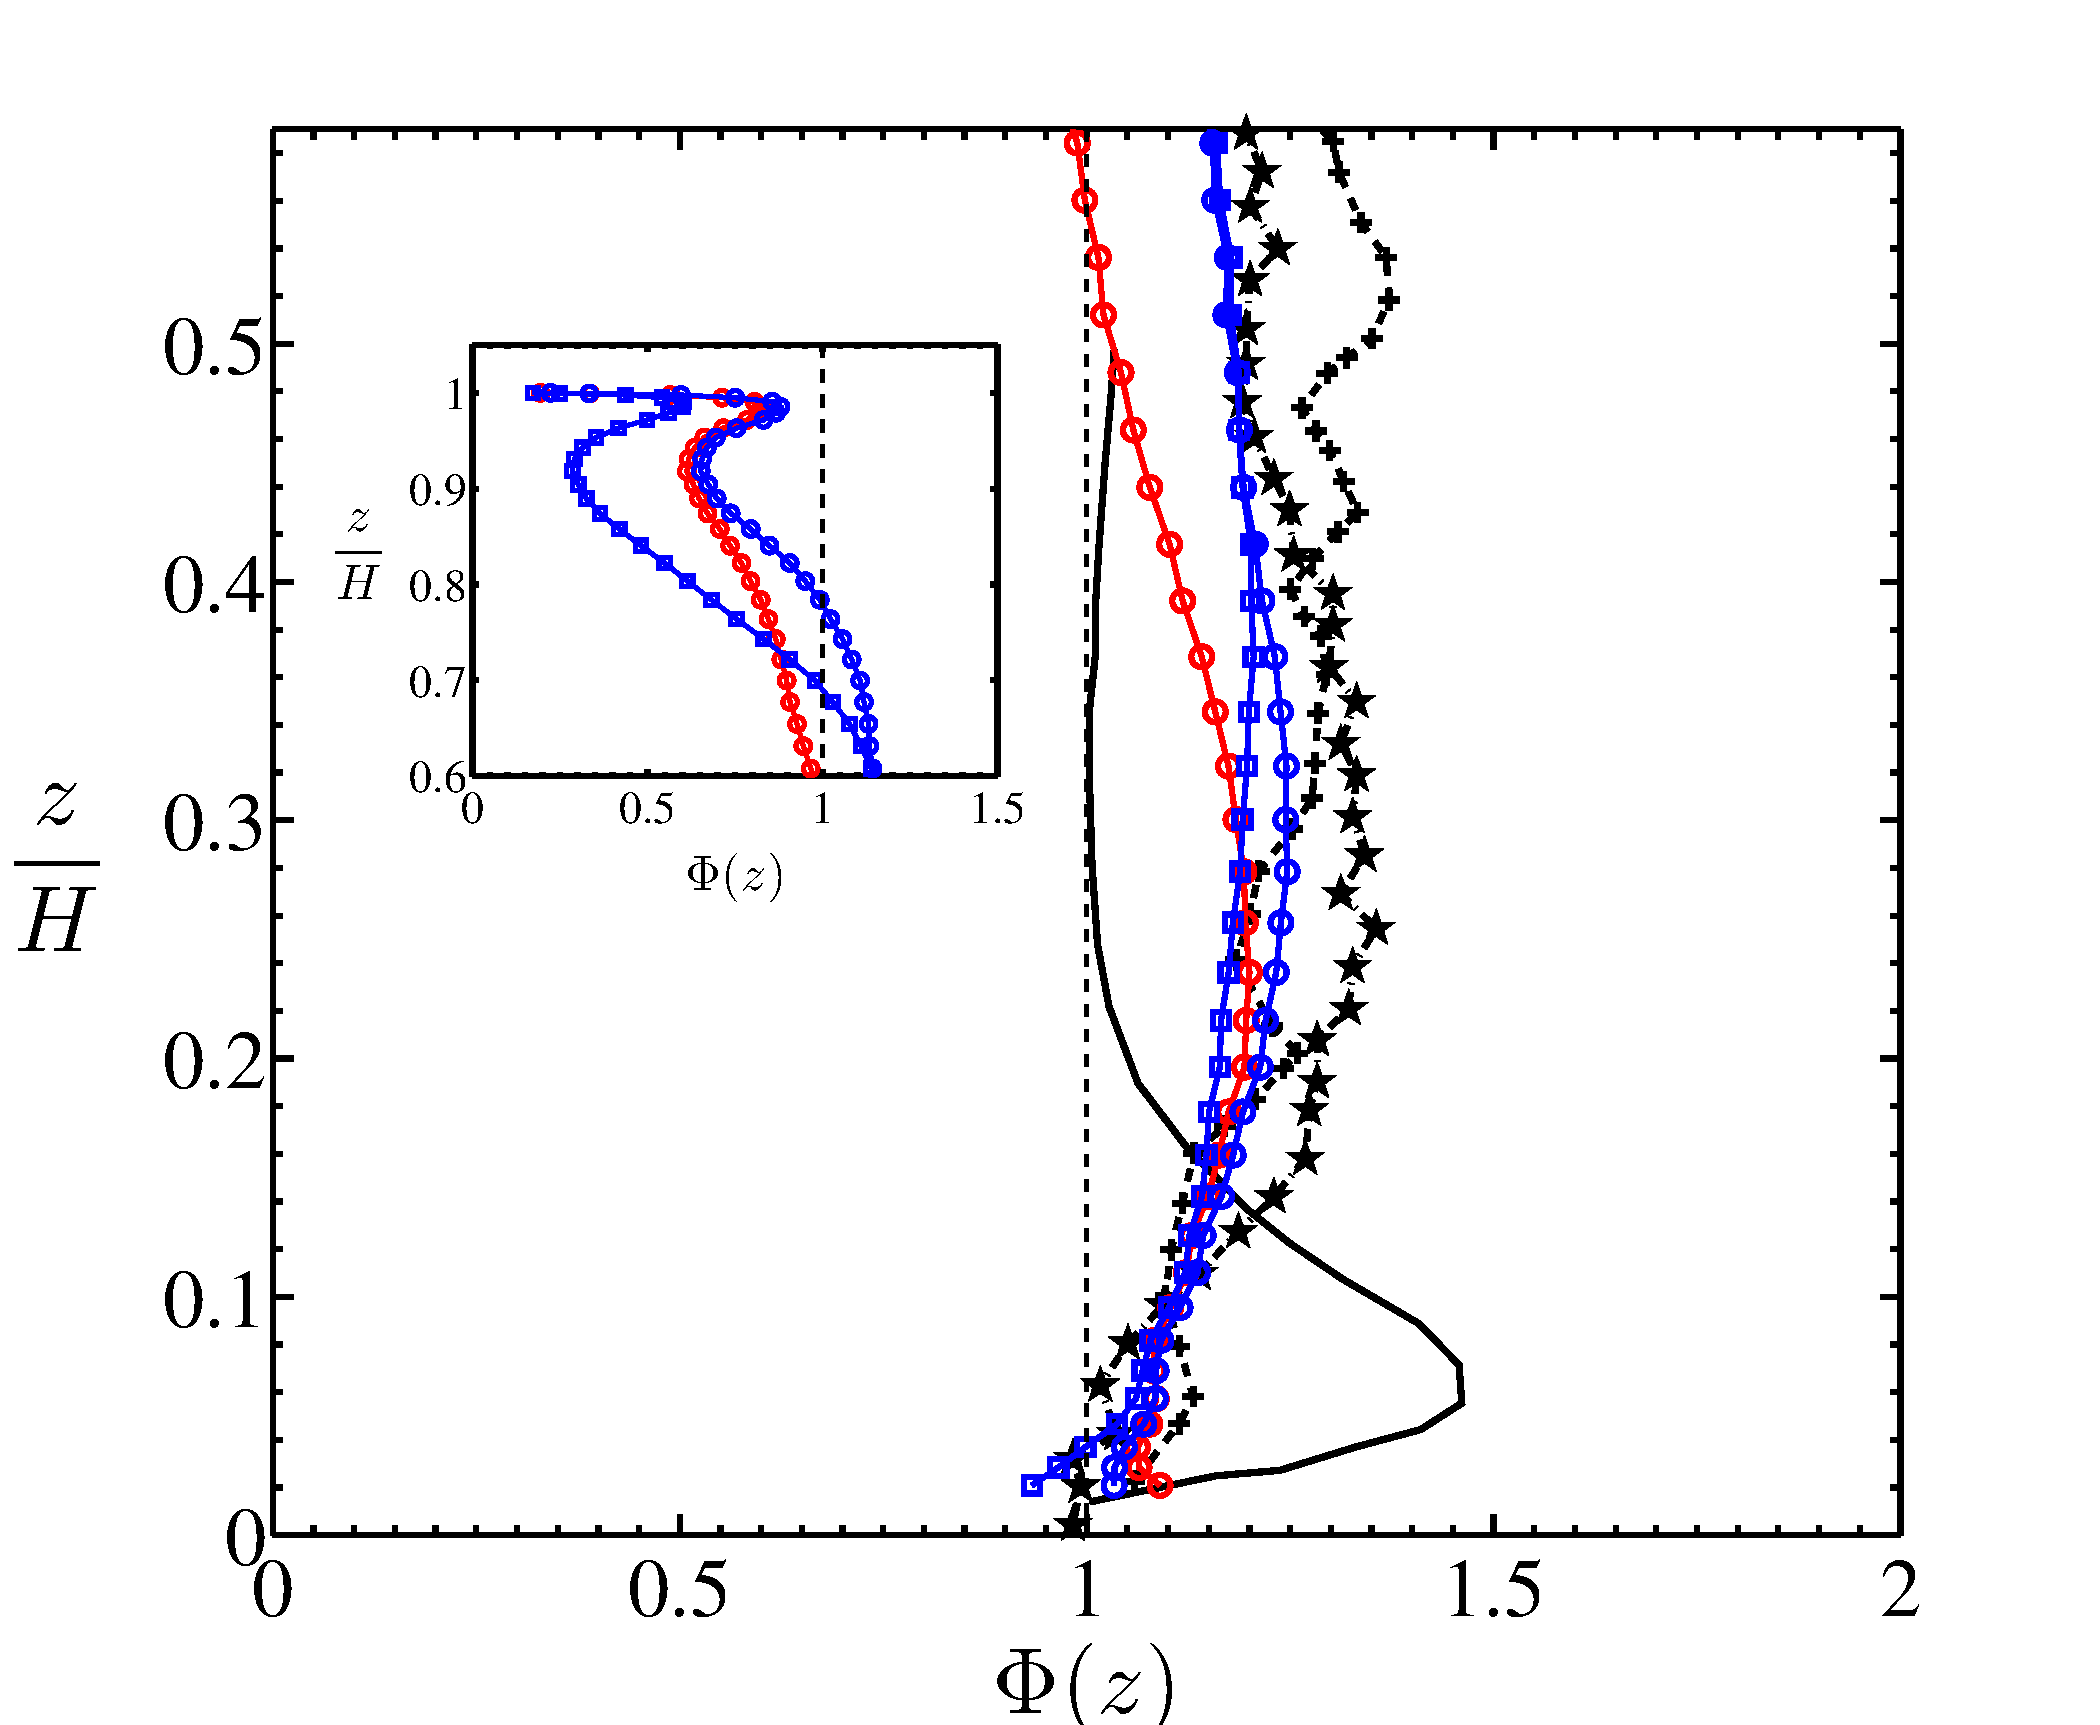
\includegraphics[width = 0.75\linewidth]{Fig3/gradient_filt_n05.pdf}        
        \caption[$\Phi(z)$, Case $VIII-X$]{Non dimensinonal mean streamwise velocity gradient $\phi(z)$ vs $z/H$. Red, Blue curves: current simulations $VIII-X$ {($n = 0.5, \ C_0 = 0.19$)}; Black curves from the literature~\cite{porte1fun,bou1}. Red $\circ$, $k_{c}=2$; Blue $\circ$, $k_{c} = 4$; Blue $\Box$, $k_{c} = 6$. Black $+$ scale dependant dynamic Smagorinsky for Port$\acute{e}$-Agel et al.~\cite{porte1fun}; $-$ , standard Smagorinsky, $\star$, Lagrangian scale dependant dynamic Smagorinsky with filtering, Bou-Zeid et. al~\cite{bou1}}\label{fig:statb}
\end{figure}

\begin{figure}
\centering
        \begin{subfigure}[t]{0.75\textwidth}
                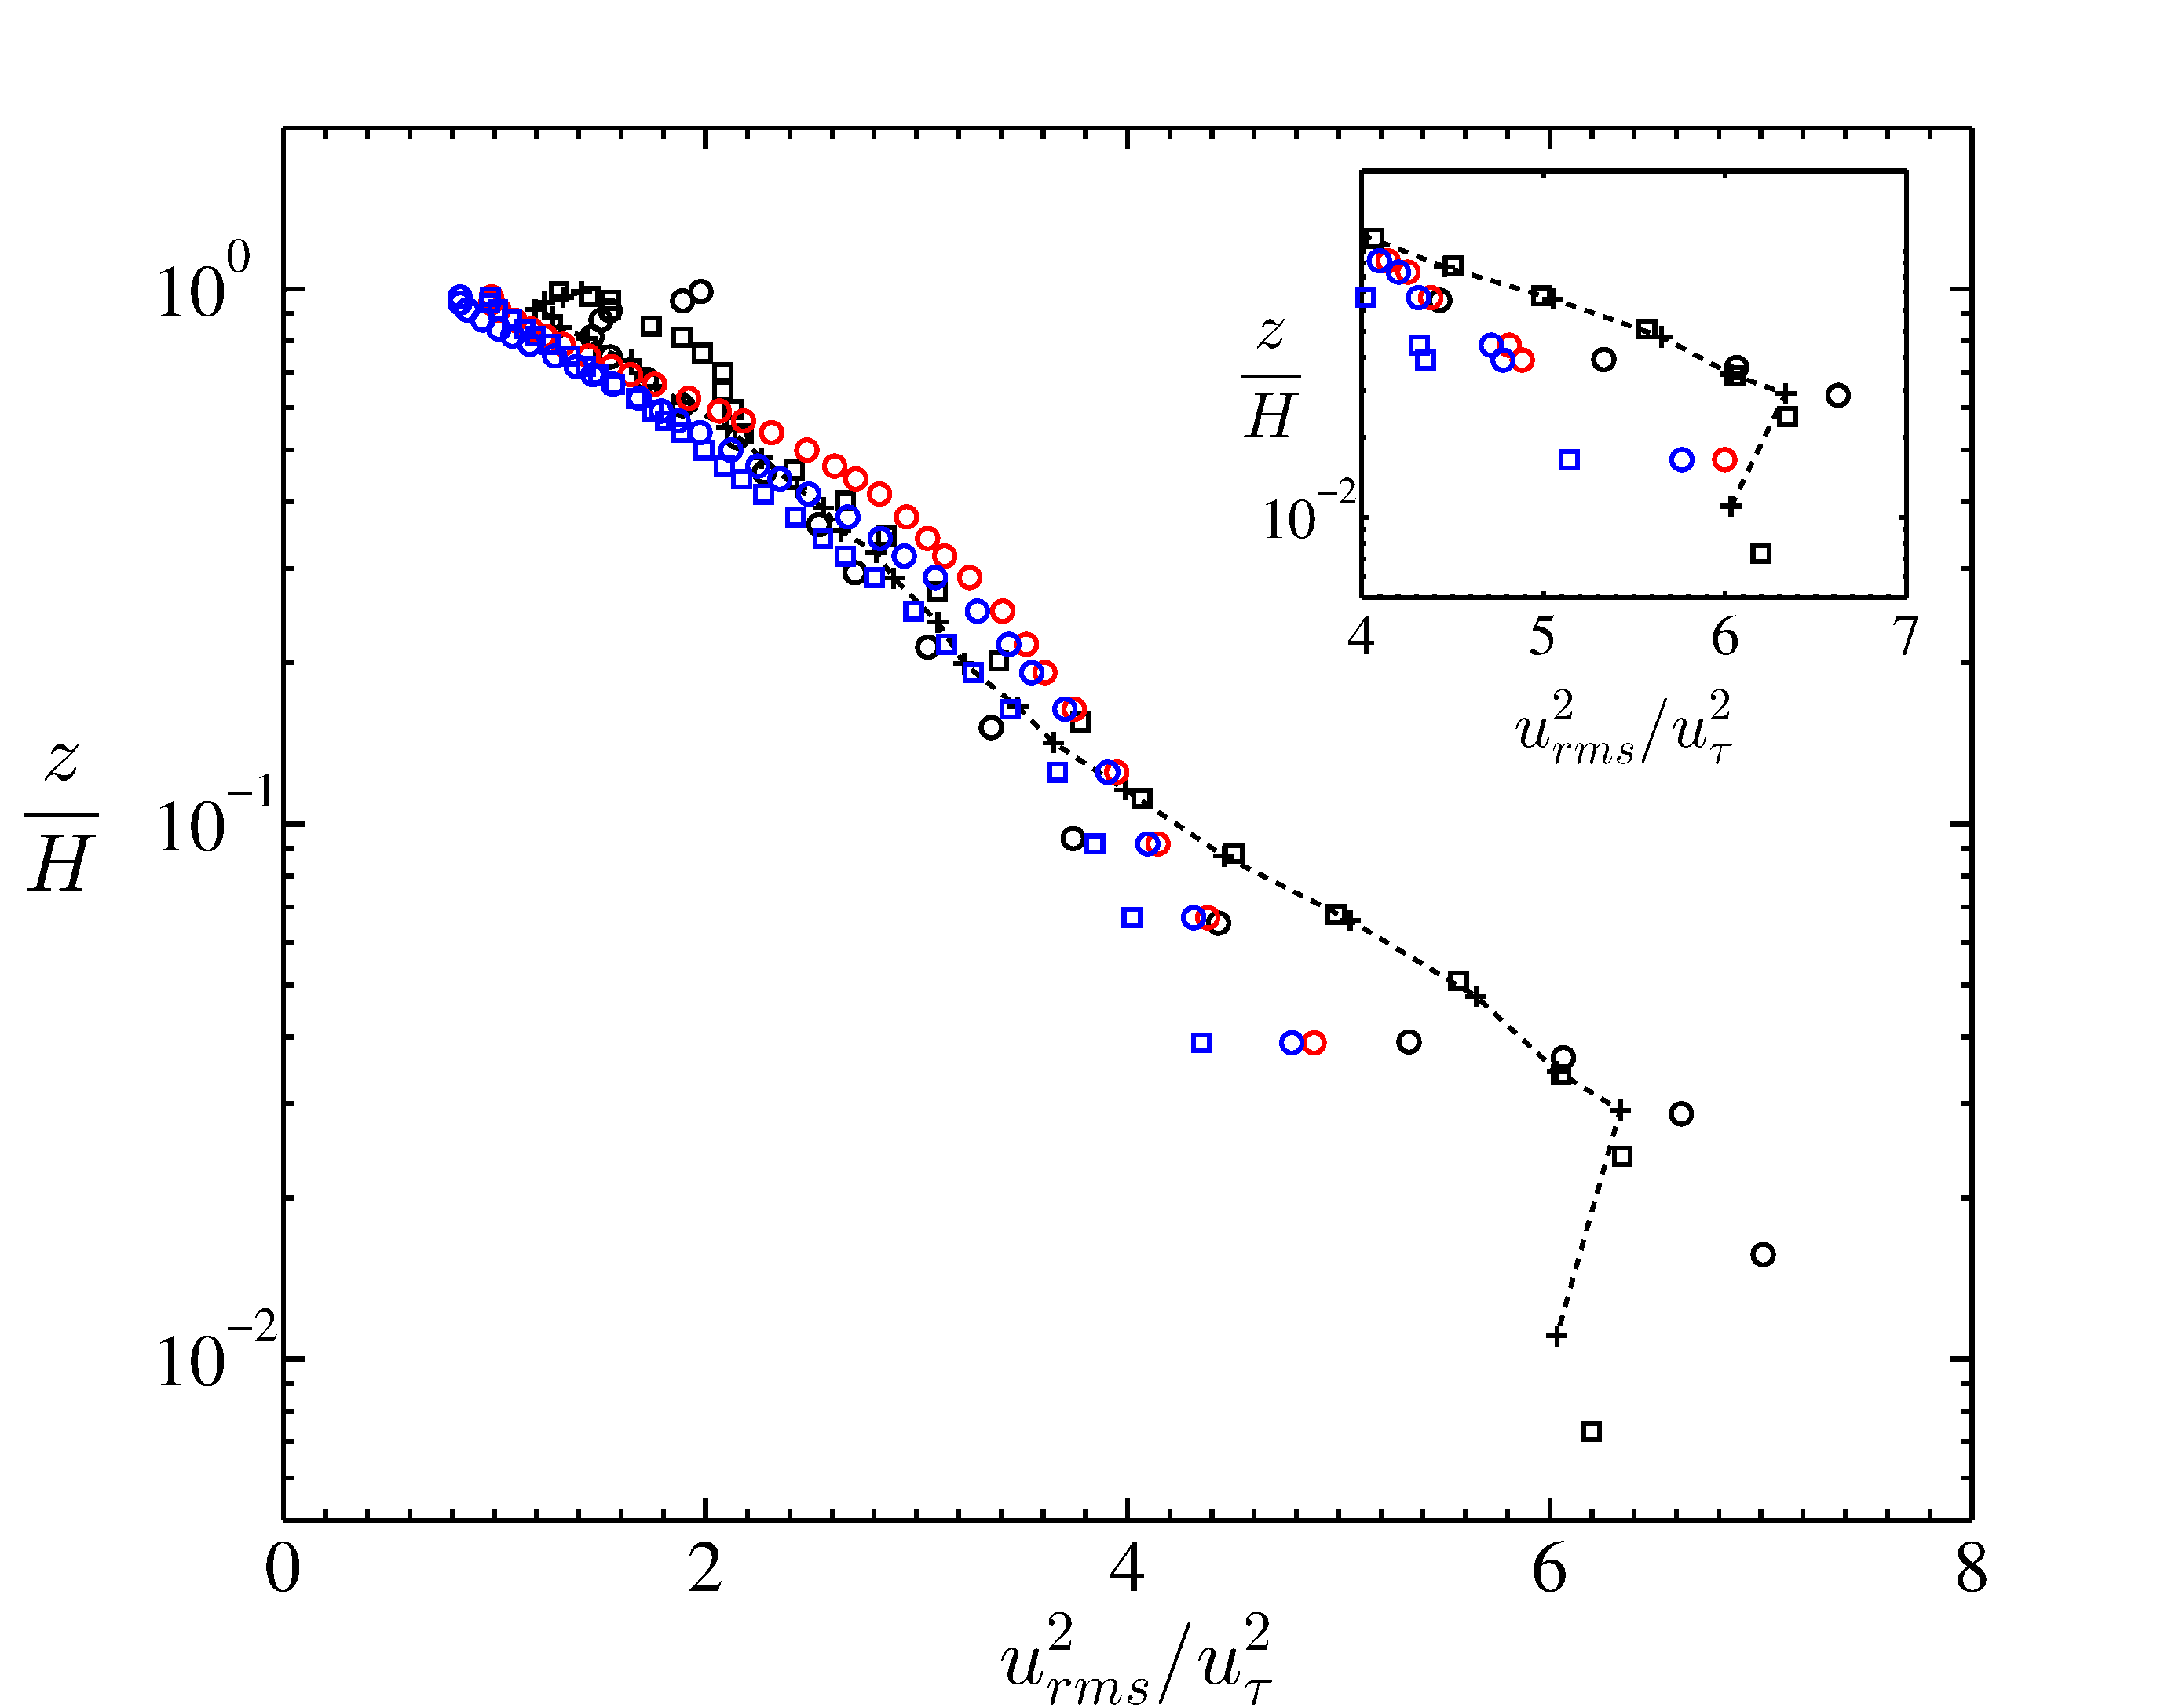
\includegraphics[width=\linewidth]{Fig3/urms_filter_n05.pdf}
                \caption{}
                \label{fig:urms1}
        \end{subfigure}
        \centering
        \begin{subfigure}[t]{0.75\textwidth}
                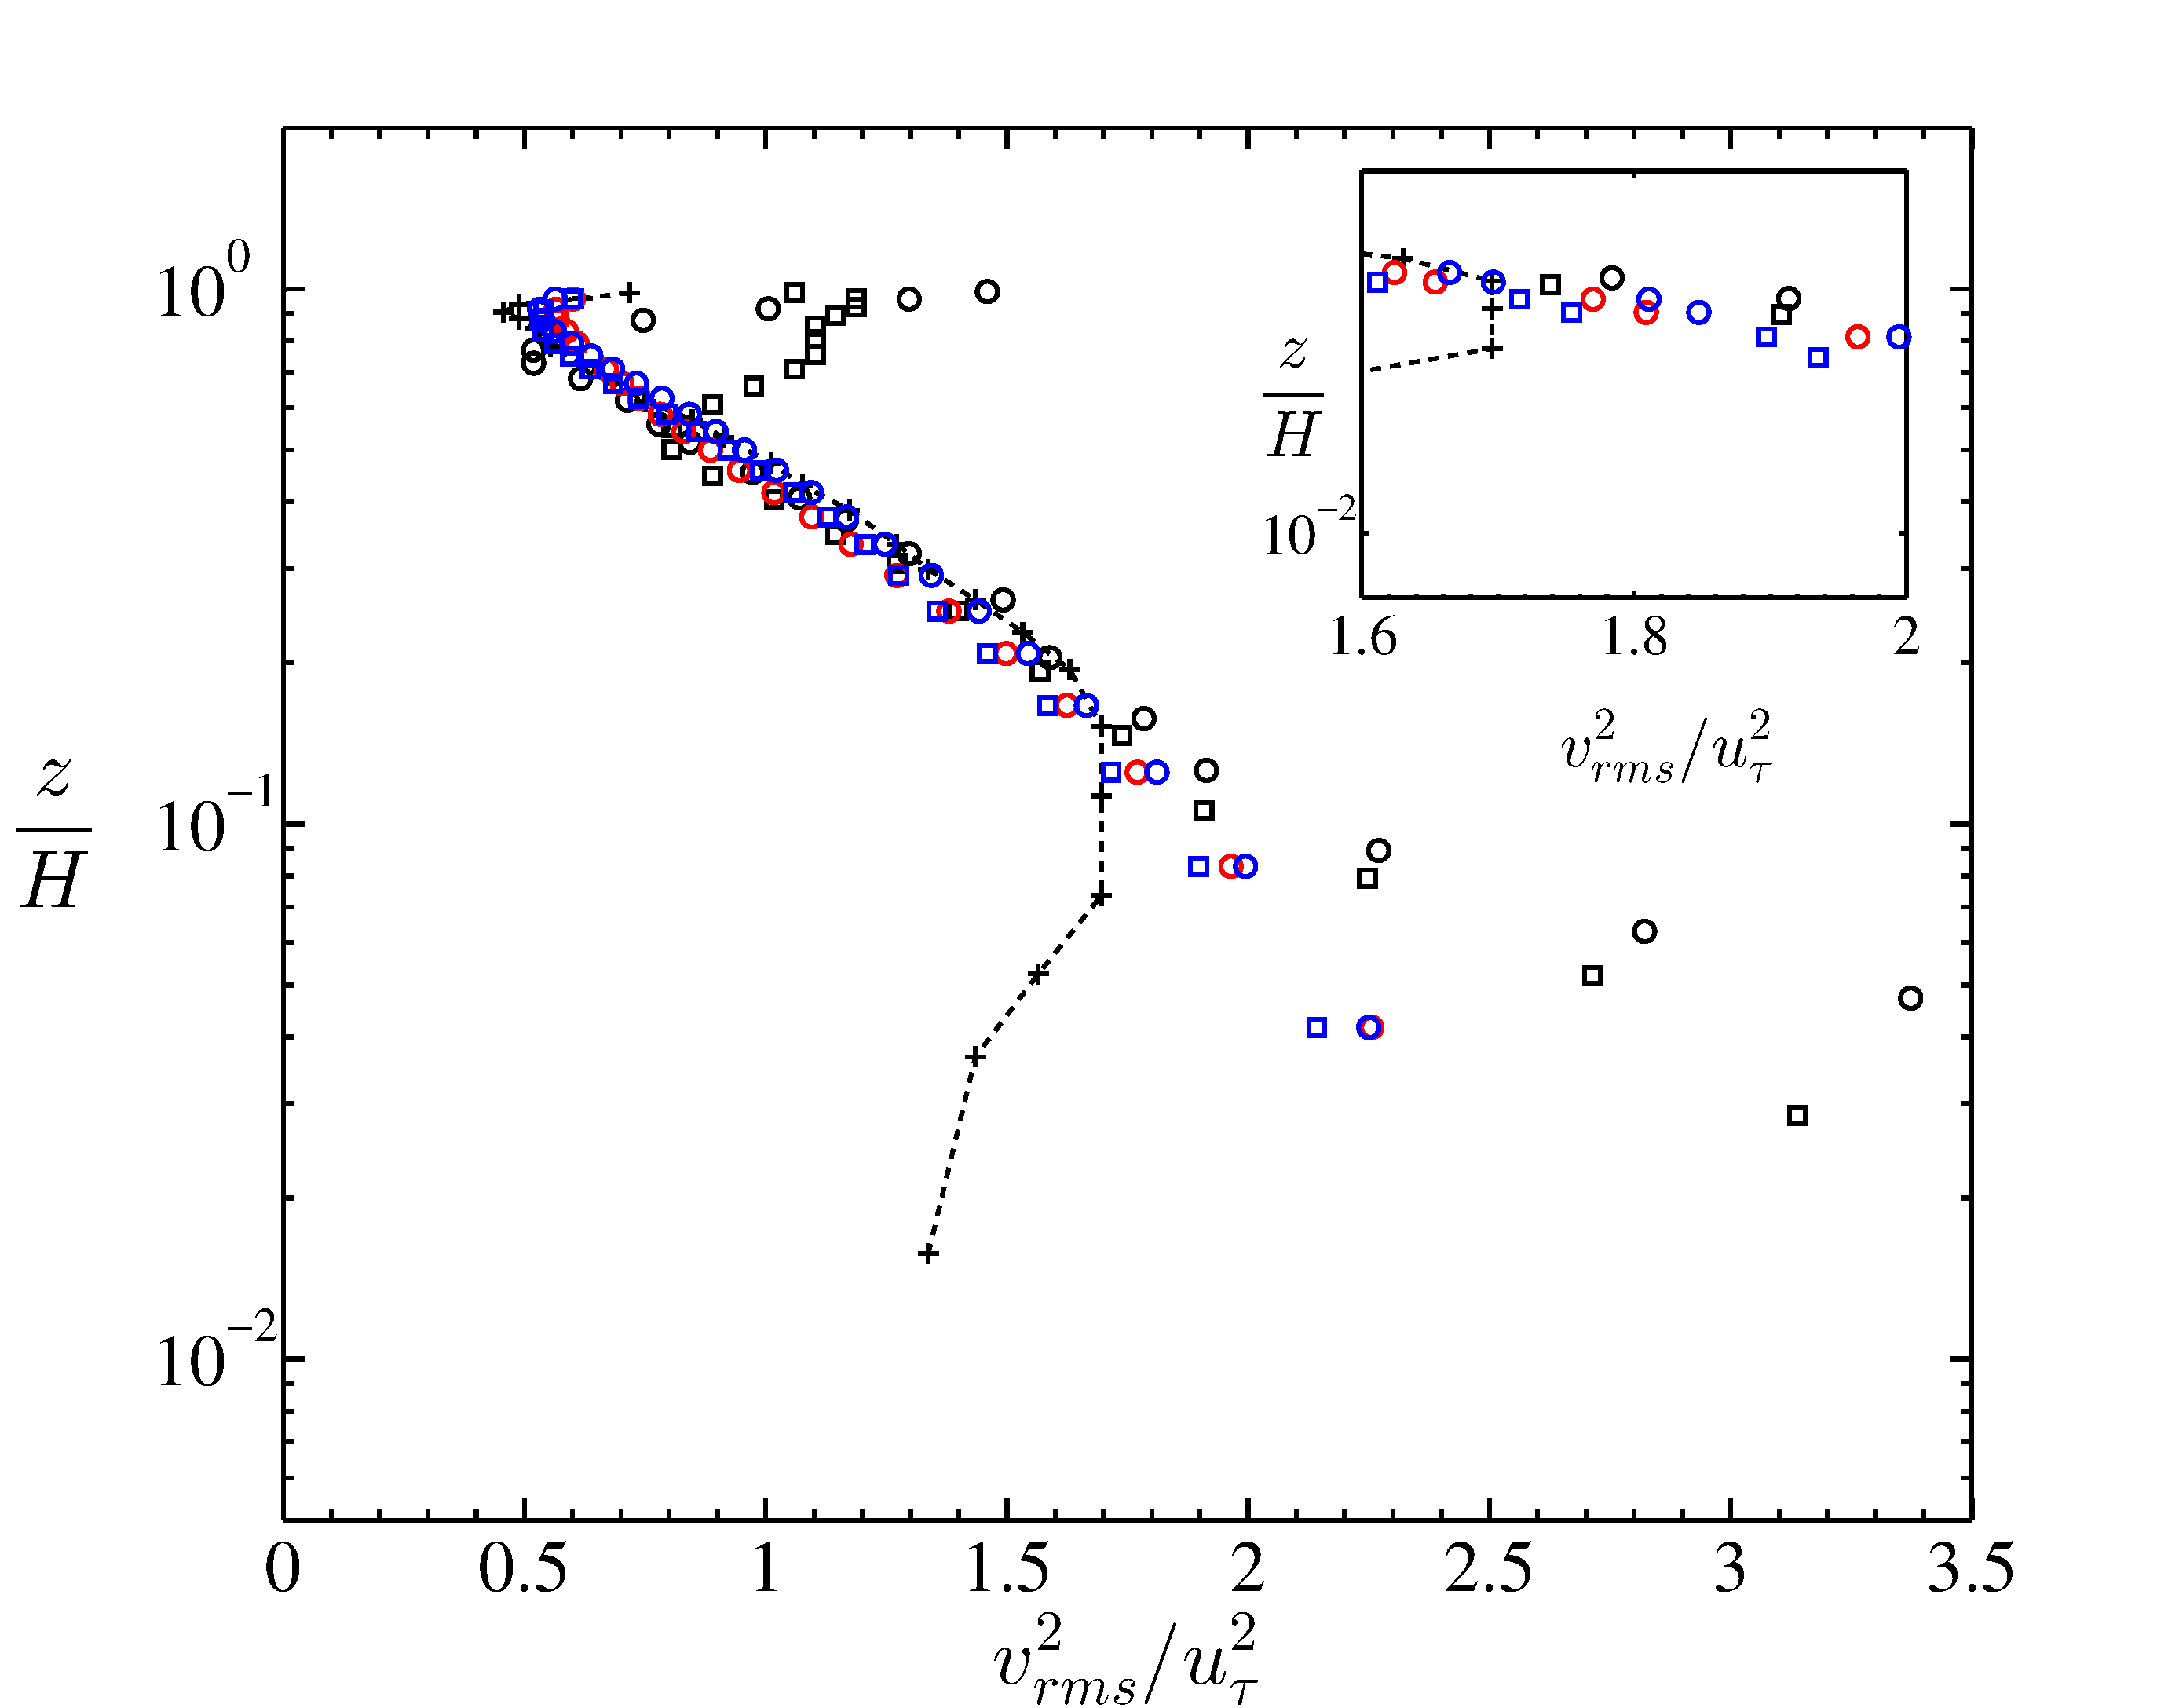
\includegraphics[width=\linewidth]{Fig3/vrms_filter_n05.pdf}
                \caption{}
                \label{fig:vrms1}
        \end{subfigure}
        \caption[Second order statistics $u_{rms}, \ v_{rms}$, Case $VIII-X$]{Second order statistics for ABL simulations: Case $VIII-X$ . (a) $u_{rms}$ (b) $v_{rms}$ . Red, Blue curves: current simulations $VIII-X$ ($n = 0.5, \ C_0 = 0.19$);  Red $\circ$, $k_{c}=2$; Blue $\circ$, $k_{c} = 4$; Blue $\Box$, $k_{c} = 6$.  Black $-+$, standard Smagorinsky ($C_s = 0.10, n = 2$)  {for Port$\acute{e}$-Agel et al.~\cite{porte1fun}} and black $\Box$ scale dependant dynamic Smagorinsky for Port$\acute{e}$-Agel et al.~\cite{porte1fun}.}\label{fig:stat021}
\end{figure}
\begin{figure}
        \centering
        \begin{subfigure}[t]{0.75\textwidth}
                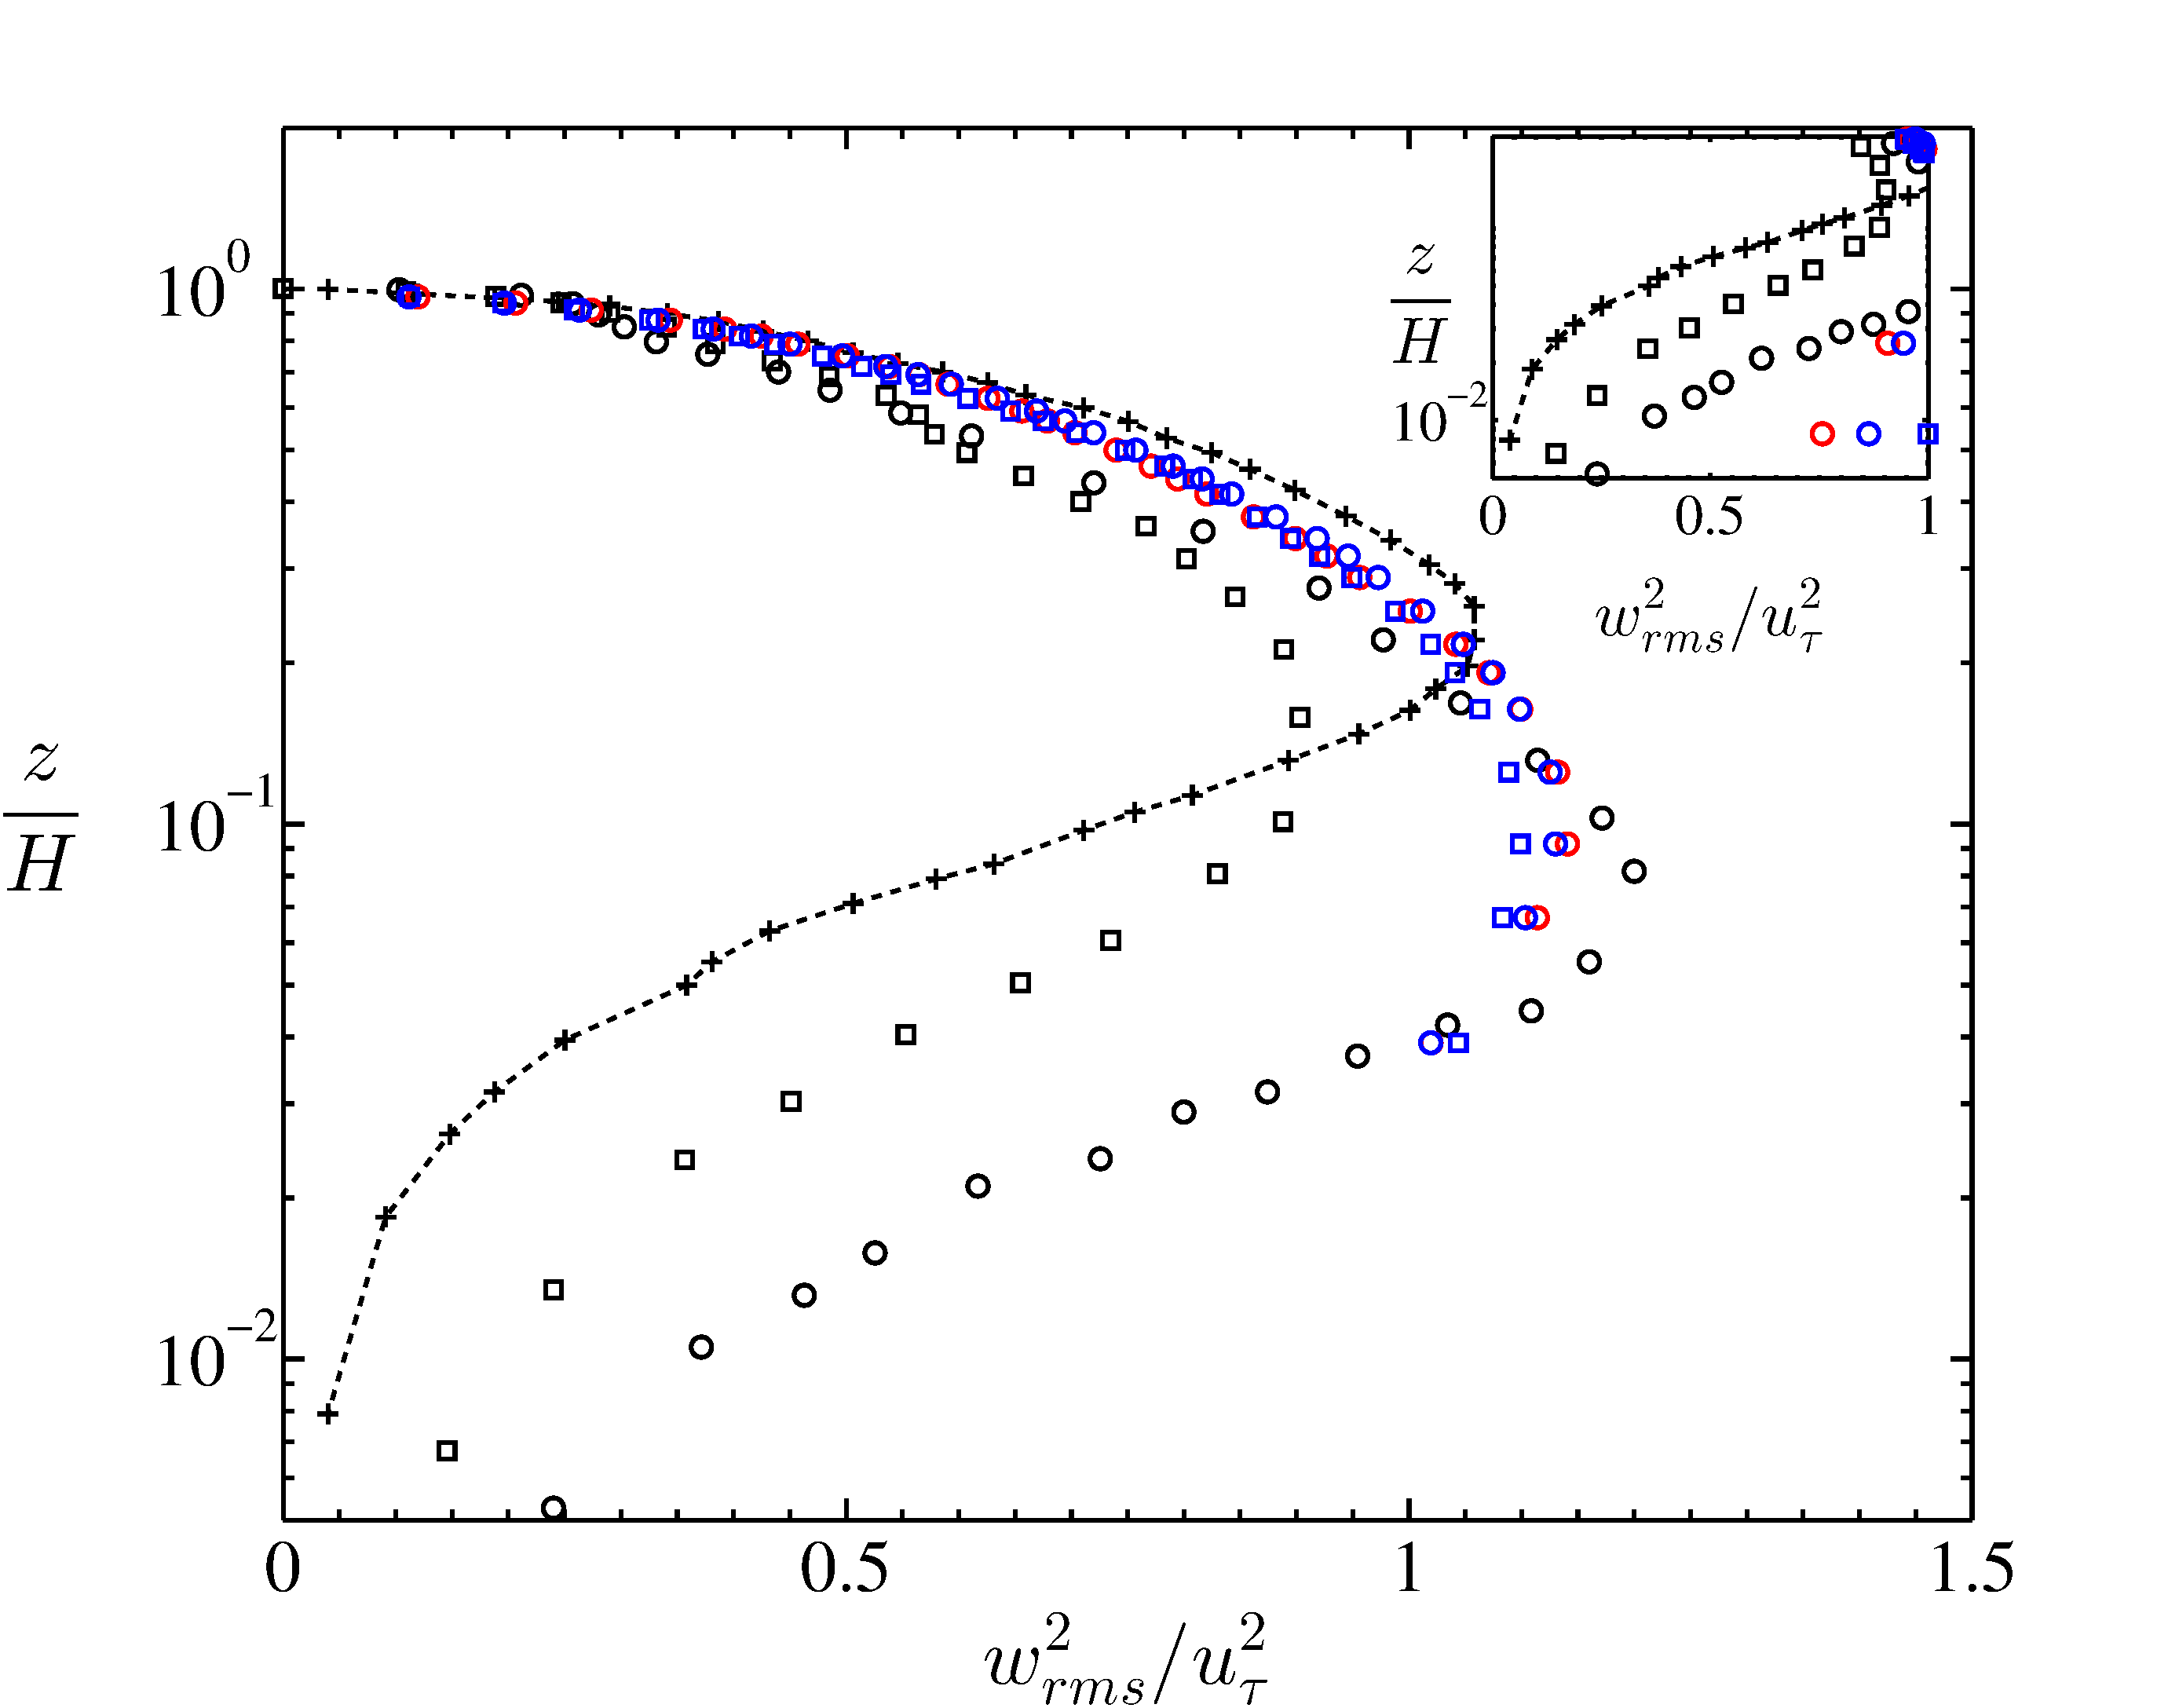
\includegraphics[width=\linewidth]{Fig3/wrms_filter_n05.pdf}
                \caption{}
                \label{fig:wrms1}
        \end{subfigure}
        \centering
        \begin{subfigure}[t]{0.75\textwidth}
                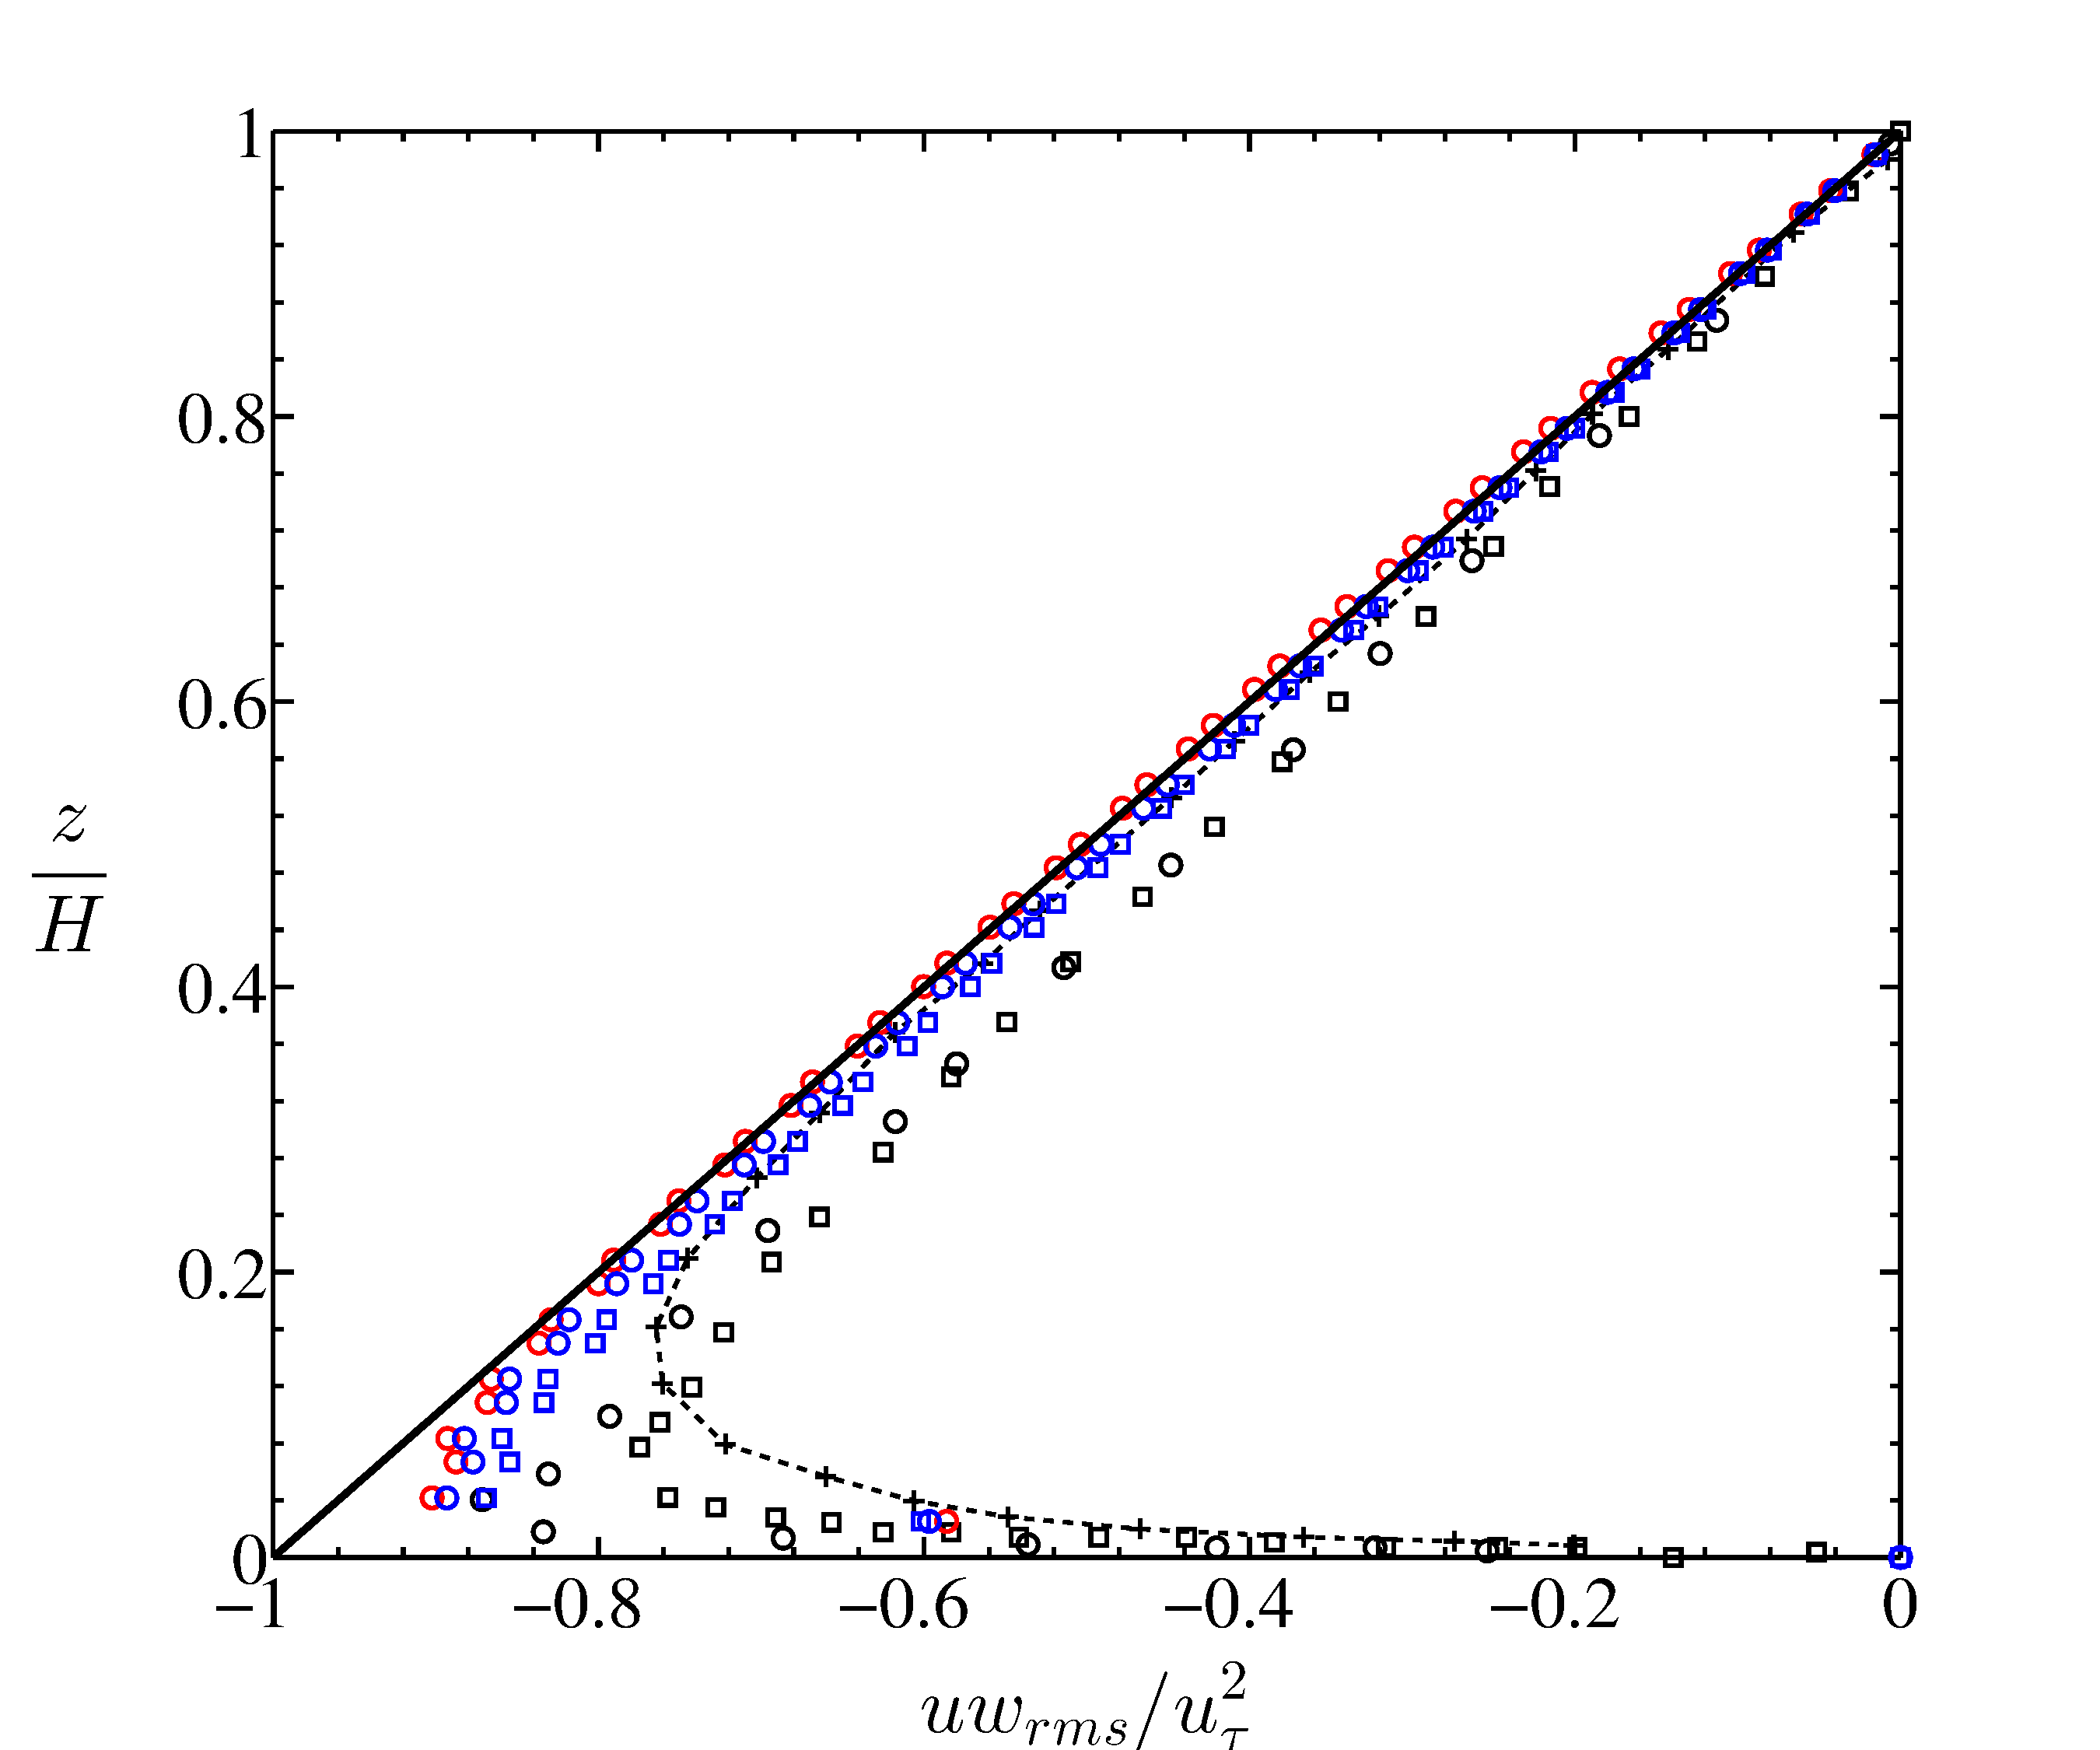
\includegraphics[width=\linewidth]{Fig3/uwrms_filter_n05.pdf}
                \caption{}
                \label{fig:uwrms1}
        \end{subfigure}%
        \caption[Second order statistics $w_{rms}, \ uw_{rms}$, Case $VIII-X$ ]{Second order statistics for ABL simulations: Case $VIII-X$ . (a) $w_{rms}$ (b) $uw_{rms}$ . Red, Blue curves: current simulations $VIII-X$ ($n = 0.5, \ C_0 = 0.19$);  Red $\circ$, $k_{c}=2$; Blue $\circ$, $k_{c} = 4$; Blue $\Box$, $k_{c} = 6$.  Black $-+$, standard Smagorinsky ($C_s = 0.10, n = 2$) {for Port$\acute{e}$-Agel et al.~\cite{porte1fun}} and black $\Box$ scale dependant dynamic Smagorinsky for Port$\acute{e}$-Agel et al.~\cite{porte1fun}. Solid black line in (b) is the ideal linear trend of non-dimensional total stress.}\label{fig:stat022}
\end{figure}

\subsection{A note on Log Layer Mismatch}\label{lotw}
The term ``log-layer mismatch" has been found in the papers by Brasseur {and Wei}~\cite{brass},  Wu $\&$ Meyers~\cite{meyers_err} and Meyers~\cite{meyers2} but {its} detrimental effects have been seen in all LES results of high Reynolds number turbulent boundary layer flow~\cite{sull,pio2,porte1fun,bou1,chow,temp2}. The effect of ``log-layer mismatch", as also discussed above, is the deviation of the mean velocity gradient from the expected logarithmic trend in the near-wall region ($\Phi(z) > 1$ and usually shows a peak structure at $z/H < 0.1$), which has been partially addressed by having a proper choice of SGS model~\cite{mason,porte1fun,bou1} or explicit filtering in the wall closure model~\cite{bou1,meyers_err,meyers2} or using more complicated techniques like optimal control theory~\cite{temp2}, designing high accuracy zones for law of {the} wall~\cite{brass} or blending functions in self-adaptive models~\cite{meyers2} .
To understand the fundamental cause of "log-layer mismatch" we resort to Figure~\ref{fig:hiRe} where we plot $\Phi(z) = \kappa z/u_{\tau} dU/dz$ vs $z/\delta$, for high $Re$ channel flow DNS~\cite{lee2} with $\delta$ being the half channel width. We note, that  similar peaked structures in Figure~\ref{fig:hiRe} (we would call them ``log law deviation" subsequently to differentiate between "log-layer mismatch" in ABL) can be seen, as we have  observed in Figures~\ref{fig:stata},~\ref{fig:statba} for rough-wall neutral atmospheric boundary layer for high $Re$. It is not hard to relate those deviations from $\Phi(z) = 1$ in Figure~\ref{fig:hiRe}, due to the presence of physical viscous sub-layer where log-law does not hold. With increasing $Re_{\tau}$, there is an increasing separation of outer and inner scales $\delta/\delta_{\nu}$~\cite{pope,balad}, where $\delta_{\nu} = \nu/u_{\tau}$. Consequently, since $\delta$ is fixed in all DNS simulations (Figure ~\ref{fig:hiRe}), increasing $Re_{\tau}$ would require the shrinkage of inner scales $\delta_{\nu}$, which does not minimize the``log-law deviations" at all but rather makes the peaks of those deviation thinner and  shifts them more towards the wall in outer scale $z/\delta$, while the peaks remain at the same locations with same magnitudes in the inner scale $z^{+}$, normalized with $\delta_{\nu}$. Consequently, the more the peak shifts towards the wall, the more quickly $\Phi(z)$ becomes closer to 1, i.e. at much lower value of $z/\delta$.  It is thus not surprising that in standard Smagorinsky model (dissipative SGS model) with constant $C_s$ or also sometimes with wall-damped $C_s$~\cite{mason,chow} for very high $Re$ we would observe similar log-law deviations due to the presence ``unphysical / artificial viscous sublayer" with a representative length scale $\delta_{\nu_t}$, where $\nu_{t} = (C_s\Delta)^{2}\vert \widetilde{S} \vert$ is the Smagorinsky eddy viscosity. Also, the location of such peaks would scale well with $\delta_{\nu_{t}} = \nu_{t}/u_{\tau}$. Similar feature as in the argument above can actually be seen through careful observation of Figure~\ref{fig:stata},~\ref{fig:statba}. The peaks of the log-layer mismatch in those figure (current spectral element simulations) are actually closer to the wall compared to the standard Smagorinsky model of Bou-Zeid et. al~\cite{bou1}. This can be attributed from the fact that the length-scale in the artificial viscous sublayer is much smaller (contributed only by the Smagorinsky model, numerical dissipation negligible) while for~\cite{bou1} $\delta_{\nu_t}$ is much larger (probably due to the contribution of numerical dissipation and higher Smagorinsky coefficient). Additionally it can be understood, that as long as the artificial boundary layer can be formed, with eddy viscosity $\nu_t$, the log-layer mismatch would persist irrelevant of the fact whether $nu_{t}$ is small or big. This is corroborated in the papers of Khanna and Brasseur~\cite{khan} and Spalart~\cite{spal2}, who observed that refining vertical resolution actually shifted the ``log-layer mismatch" downards towards the wall which can be attributed to the decrement yet persistance of the numerical dissipation in the grid. (similar as in Figure~\ref{fig:hiRe}) It is only with a careful design of $nu_{t}$, we can stop the artificial / unphysical layer to form itself, resulting in proper log-layer predictions. These ideas are along the lines of the Log-law analysis made by Brasseur and Wei~\cite{brass}, and can be referred for further details. A quick calculation of  the parameters $\mathfrak{R}-R_{LES}-N_{\delta}$ in Table~\ref{table:brass} as suggested by Brasseur and Wei~\cite{brass} along with their critical values have been registered. The parameters (See details in~\cite{brass}) should be greater than the critical values to avoid log-layer mismatch, and it is not surprising that only models with $n = 1/2$ and indepedant of the filtering modes $k_c$ consistently qualify their tests and thus can avoid ``log-layer mismatch". The bottom line is simply decreasing of $C_s\Delta$ in the Smagorinsky coefficient would never minimize log-layer mismatch as its origin does not lie on extra-dissipative Smagorinsky model, but rather an unphysical near wall dissipation in the first place. These discussions are corroborated by the fact that the biggest challenge reported in representing the near wall logarithmic trends (also the near-wall features) on a relatively co{a}rse LES grid  is that the {numerical discretization errors} near wall start \textbf{interfering} with the physical modelling and affecting the results of the resolved statistics~\cite{cabot2,brass,meyers2}.  
 %Additionally it was also observed that in the first grid point of the finite difference scheme large errors of velocity gradient deviating from the logarithmic trends crop in, and are alleviated by simply brute forcing the logarithmic gradient at the first grid point~\cite{porte1fun,meyers2}. 
\begin{table}[ht] 
\centering % used for centering table 
\begin{tabular}{c c c c} % centered columns (4 columns) 
\hline\hline    %inserts double horizontal lines 
Case & $\mathfrak{R}$  & $R_{LES}$ & $N_{\delta}$   \\ [0.5 ex] % inserts table 
%heading 
\hline  % inserts single horizontal line 
III & 0.0599 & 436 & 169 \\
VI & 0.1517 & 474 & 169 \\
IX & 1.6454 & 1090 & 169 \\
\hline
VIII & 1.6811 & 1105 & 169 \\
IX & 1.6454 & 1090 & 169 \\
X & 1.5835 & 1064 & 169 \\
\hline \\ [1 ex]
\end{tabular} 
\caption[HAZ parameters of Brasseur and Wei (2010)]{Estimation of three parameters suggested by Brasseur and Wei~\cite{brass} in our current model to estimate the High-Accuracy-Zone. Critical parameters: $\mathfrak{R^{*}} \gtrsim 1$, $R_{LES}^{*} > 350$ and $N_{\delta}^{*} > 45-50$}  % title of Table 
\label{table:brass} % is used to refer this table in the text 
\end{table} 
% May be conclusion: decouple SGS modelling error + Numerical discretization error
To summarize, as pointed out by Brasseur and Wei~\cite{brass}, we would like to emphasize that the persistance of log-scaling is essentially the dominance of intertial scales ($u_{\tau}, z$) over viscous scales (molecular, SGS dissipation/ numerical) and also scales imposed by the roughness element $z_0$. Mismatch would occur, if any other scales, dominates over the inertial scaling. It is at this bottleneck, that the spectral element method plays a crucial role in modelling the high $Re$ turbulent boundary layer flows. Using higher polynomial orders ($\sim 7$) and limited amount of tuning in the SGS models in the current simulations, we can technically put a barrier to the diffusion and dispersion errors (spurious numerical scales) percolating to the physical system involving near wall modelling. Consequently, we could address the effects of ``log layer mismatch" or the generation of an artificial viscous sublayer with a reasonable amount of success {without evoking more sophisticated dynamic-type models}.  {From Figure~\ref{fig:stat0_lotw} we observe that the SGS models with $n = \frac{1}{2}$ show much better logarithmic trends {at $z/H \sim 0.1$} as compared to $n = 1,2,3$ which manifest ``log-layer mismatch".}

\begin{figure}
\centering
\begin{subfigure}[t]{0.5\textwidth}
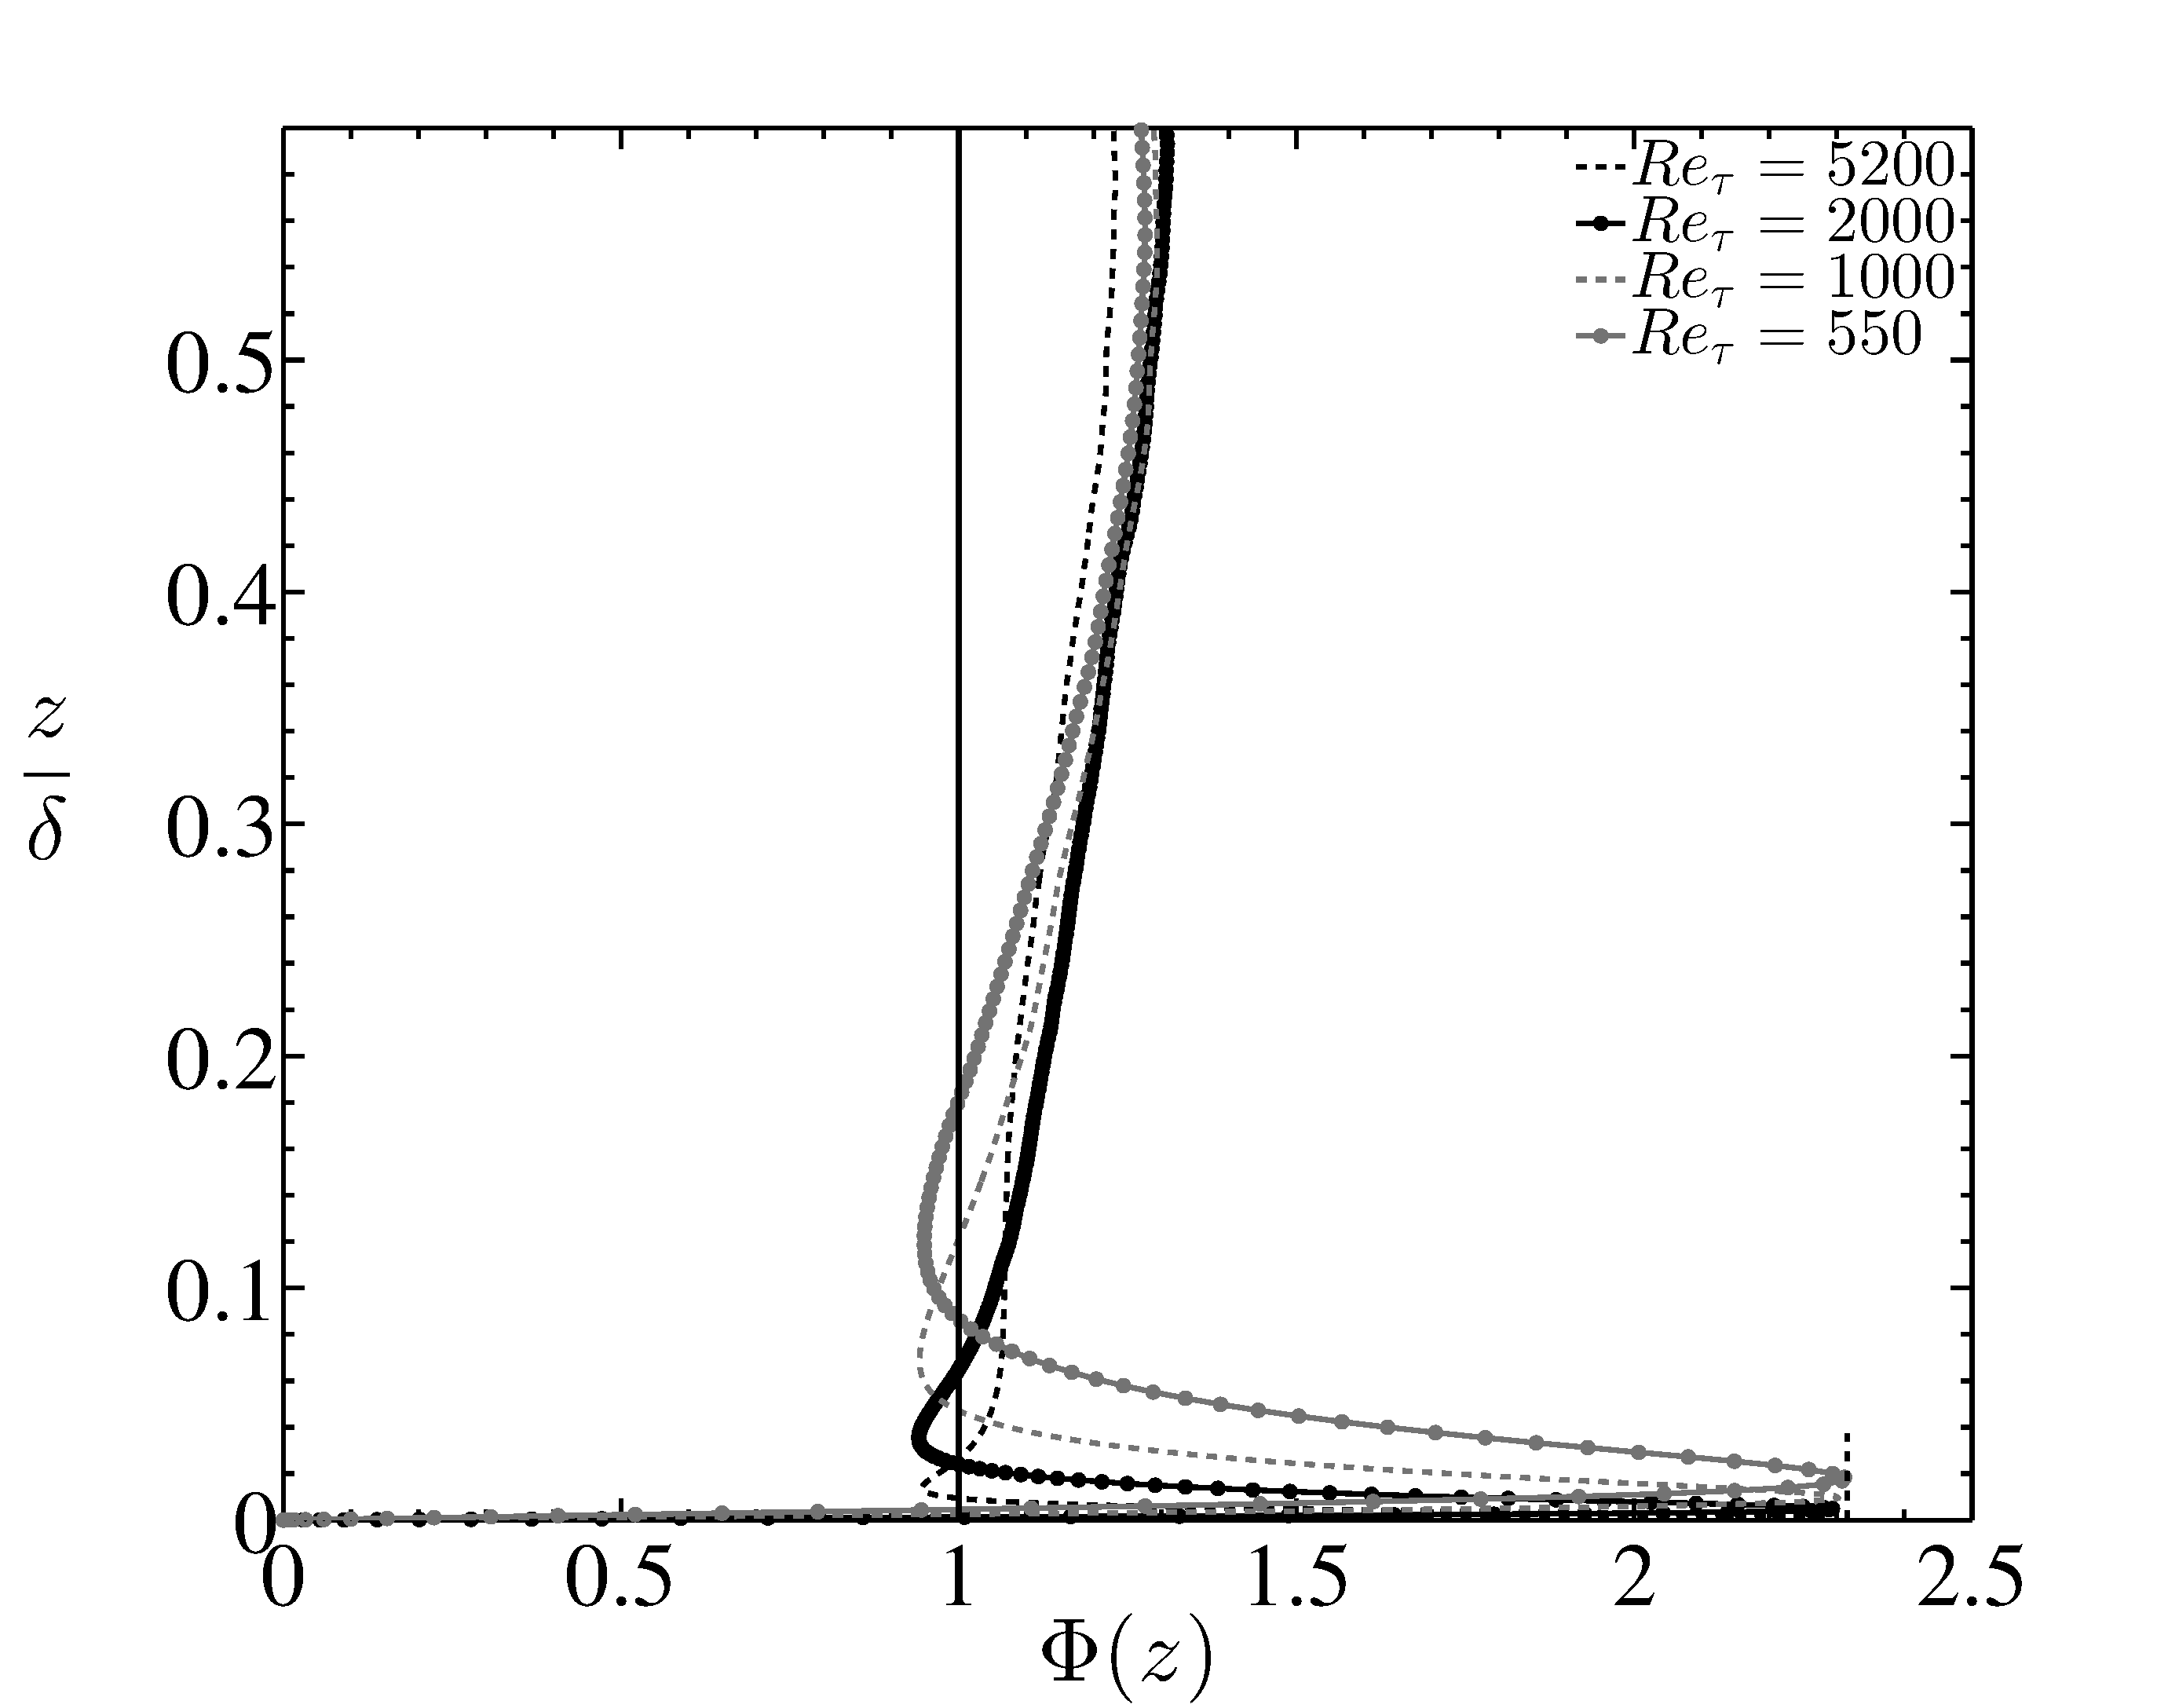
\includegraphics[width = \linewidth]{Figure/highRe.pdf}
\end{subfigure}%
\begin{subfigure}[t]{0.5\textwidth}
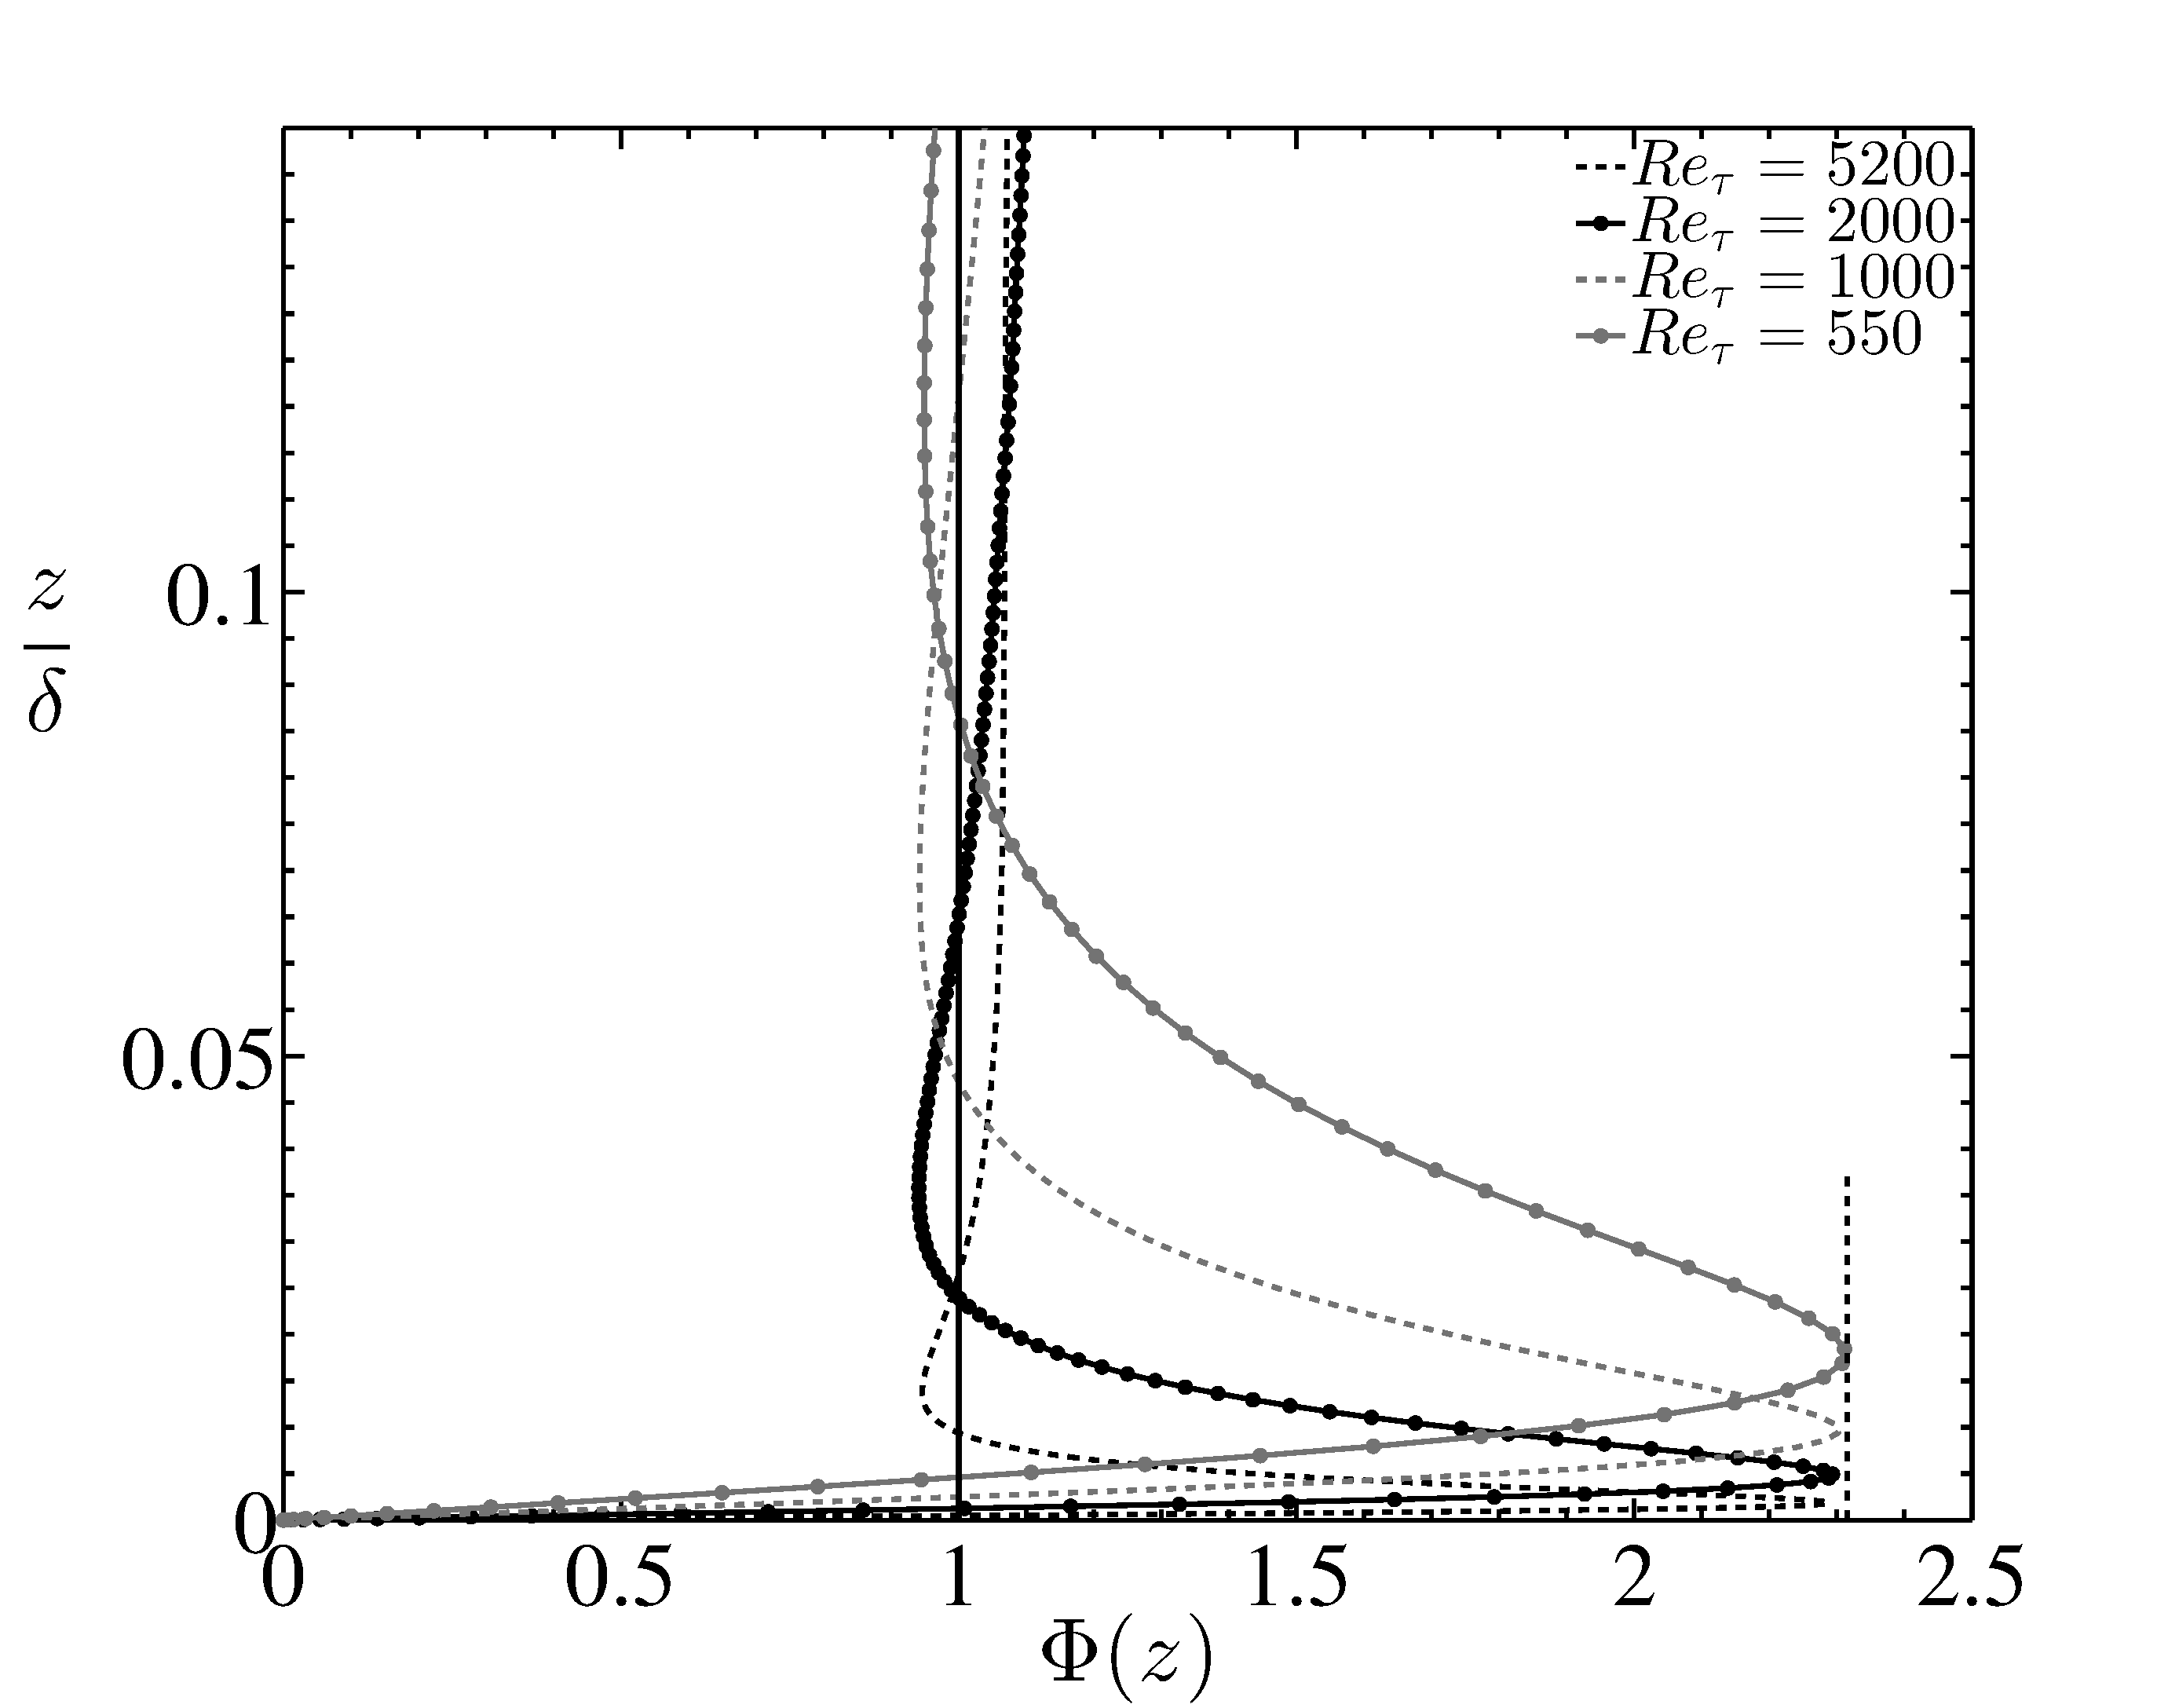
\includegraphics[width = \linewidth]{Figure/highRe2.pdf}
\end{subfigure}
\begin{subfigure}[t]{0.65\textwidth}
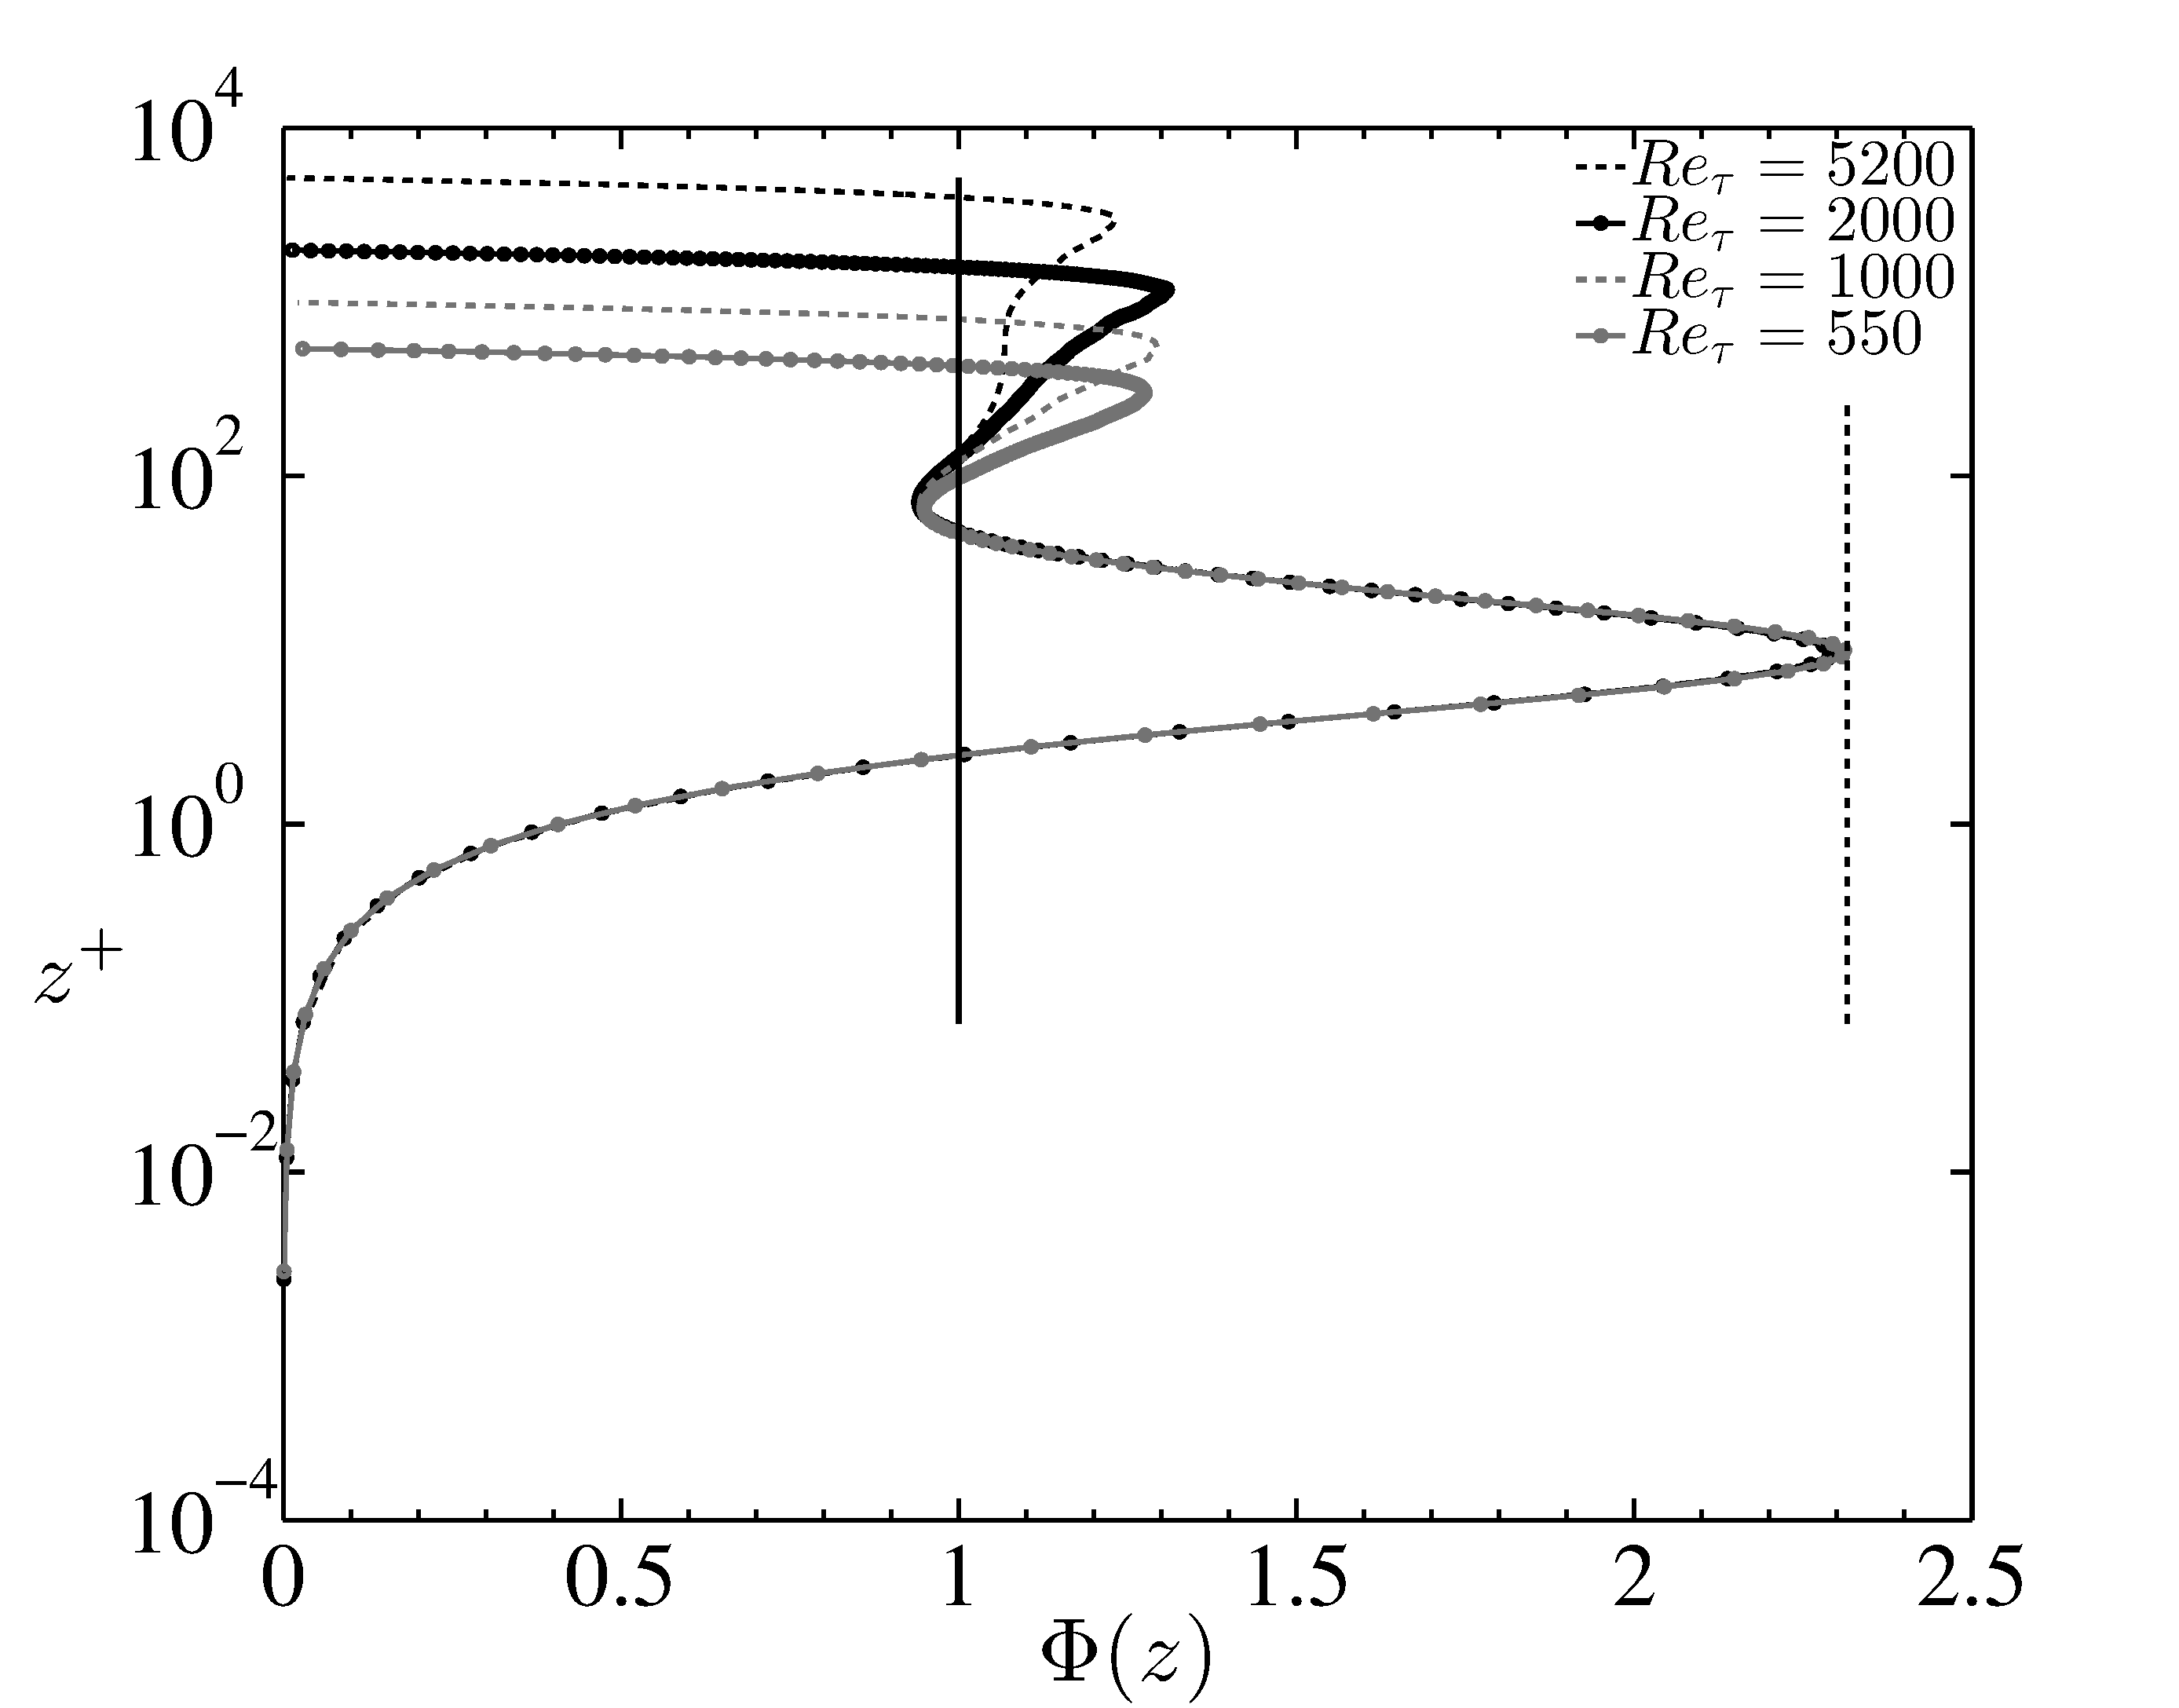
\includegraphics[width = \linewidth]{Figure/highRe2bb.pdf}
\end{subfigure}
\caption[Log-law deviation in high $Re_{\tau}$ channel flows]{High fidelity DNS simulations showing deviation of logarithmic trends $\Phi(z) \gg 1$ in the near-wall region, at very high Reynolds number channel flows.}\label{fig:hiRe}
\end{figure} 

\begin{figure}
\begin{minipage}{0.5\textwidth}
%\centering
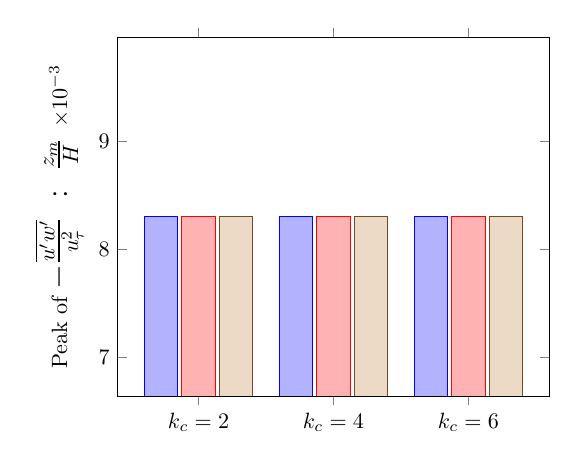
\begin{tikzpicture}[scale=0.8]
\begin{axis}[
    ybar,
    enlargelimits=0.3,
    legend style={at={(0.75,1.05)},
      anchor=north,legend columns=-1},
      ybar,
      bar width = 15pt,
    ylabel={Peak of \Large $-\frac{\overline{u'w'}}{u_{\tau}^2} \ : \ \frac{z_m}{H}$  \normalsize  $\times 10^{-3}$},
    symbolic x coords={$k_c=2$,$k_c=4$,$k_c=6$},
    xtick=data,
%    nodes near coords,
%    nodes near coords align={vertical},
    ]
\addplot coordinates {($k_c=2$,8.3) ($k_c=4$,8.3) ($k_c=6$,8.3)};
\addplot coordinates {($k_c=2$,8.3) ($k_c=4$,8.3) ($k_c=6$,8.3)};
\addplot coordinates {($k_c=2$,8.3) ($k_c=4$,8.3) ($k_c=6$,8.3)};
%\legend{I-IV,V-VII,VIII-X}
\end{axis}
\end{tikzpicture}
%\caption{Peak of normalized kinematic shear stress $-{uw_{rms}}/{u_{\tau}}^2$ in bar graph. Red: Cases I-IV $\lbrace C_0 = 0.16, n = 2 \rbrace$, Blue: Cases V-VII $\lbrace C_0 = 0.17, n = 1 \rbrace$ ,Green: Cases VIII-X $\lbrace C_0 = 0.19, n = \frac{1}{2} \rbrace$}\label{fig:bargraph}
%\captionof{figure}{Peak of normalized kinematic shear stress $-{uw_{rms}}/{u_{\tau}}^2$ in bar graph. Red: Cases I-IV $\lbrace C_0 = 0.16, n = 2 \rbrace$, Blue: Cases V-VII $\lbrace C_0 = 0.17, n = 1 \rbrace$ ,Green: Cases VIII-X $\lbrace C_0 = 0.19, n = \frac{1}{2} \rbrace$}
%\label{fig:fig2}
\end{minipage}%
\begin{minipage}{0.4\textwidth}
%\centering
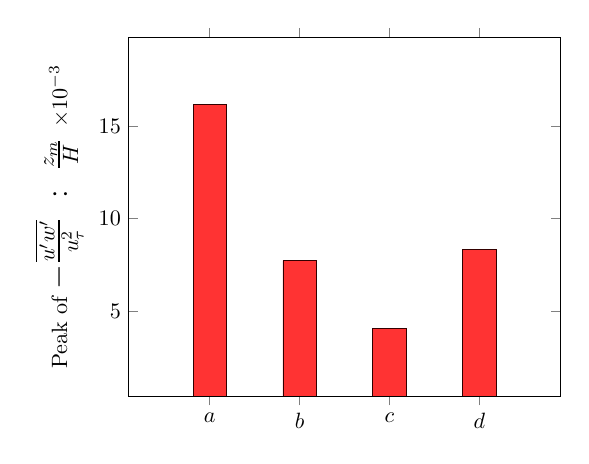
\begin{tikzpicture}[scale=0.8]
\begin{axis}[
    ybar,
    enlargelimits=0.3,
    legend style={at={(0.75,1.05)},
      anchor=north,legend columns=-1},
      ybar,
      bar width = 15pt,
    ylabel={Peak of \Large $-\frac{\overline{u'w'}}{u_{\tau}^2} \ : \ \frac{z_m}{H}$  \normalsize  $\times 10^{-3}$},
    symbolic x coords={$a$,$b$,$c$,$d$},
    xtick=data,
%    nodes near coords,
%    nodes near coords align={vertical},
    ]
\addplot[red!20!black,fill=red!80!white] coordinates {($a$,16.15) ($b$,7.72) ($c$,4.04) ($d$,8.33)};

%\legend{I-IV,V-VII,VIII-X}
\end{axis}
\end{tikzpicture}
%\caption{Peak of normalized kinematic shear stress $-{uw_{rms}}/{u_{\tau}}^2$ in bar graph. Red: Cases I-IV $\lbrace C_0 = 0.16, n = 2 \rbrace$, Blue: Cases V-VII $\lbrace C_0 = 0.17, n = 1 \rbrace$ ,Green: Cases VIII-X $\lbrace C_0 = 0.19, n = \frac{1}{2} \rbrace$}\label{fig:bargraph2}
%\captionof{figure}{Peak of normalized kinematic shear stress~\cite{porte1fun} (a) standard Smagorinsky (b) scale-dependant dynamic Smagorinsky (c) dynamic Smagorinsky }
%\label{fig:fig2}
\end{minipage}
\caption[Peak of kinematic shear stress]{\textit{Left}: Peak of normalized kinematic shear stress $-{uw_{rms}}/{u_{\tau}}^2$ in bar graph. Red: Cases I-IV $\lbrace C_0 = 0.16, n = 2 \rbrace$, Blue: Cases V-VII $\lbrace C_0 = 0.17, n = 1 \rbrace$ ,Green: Cases VIII-X $\lbrace C_0 = 0.19, n = \frac{1}{2} \rbrace$. \textit{Right}: Peak of normalized kinematic shear stress $-{uw_{rms}}/{u_{\tau}}^2$ ($a$,$b$,$c$) in Port\'{e}-Agel et. al~\cite{porte1fun}. $a$: standard Smagorinsky; $b$ scale-dependant dynamic Smagorinsky; $c$ dynamic Smagorinsky; $d$ current simulation with any set of $\lbrace C_0, \ n\rbrace$}\label{fig:peak}
\end{figure}

\begin{figure}
        \centering
        \begin{subfigure}[t]{0.5\textwidth}
                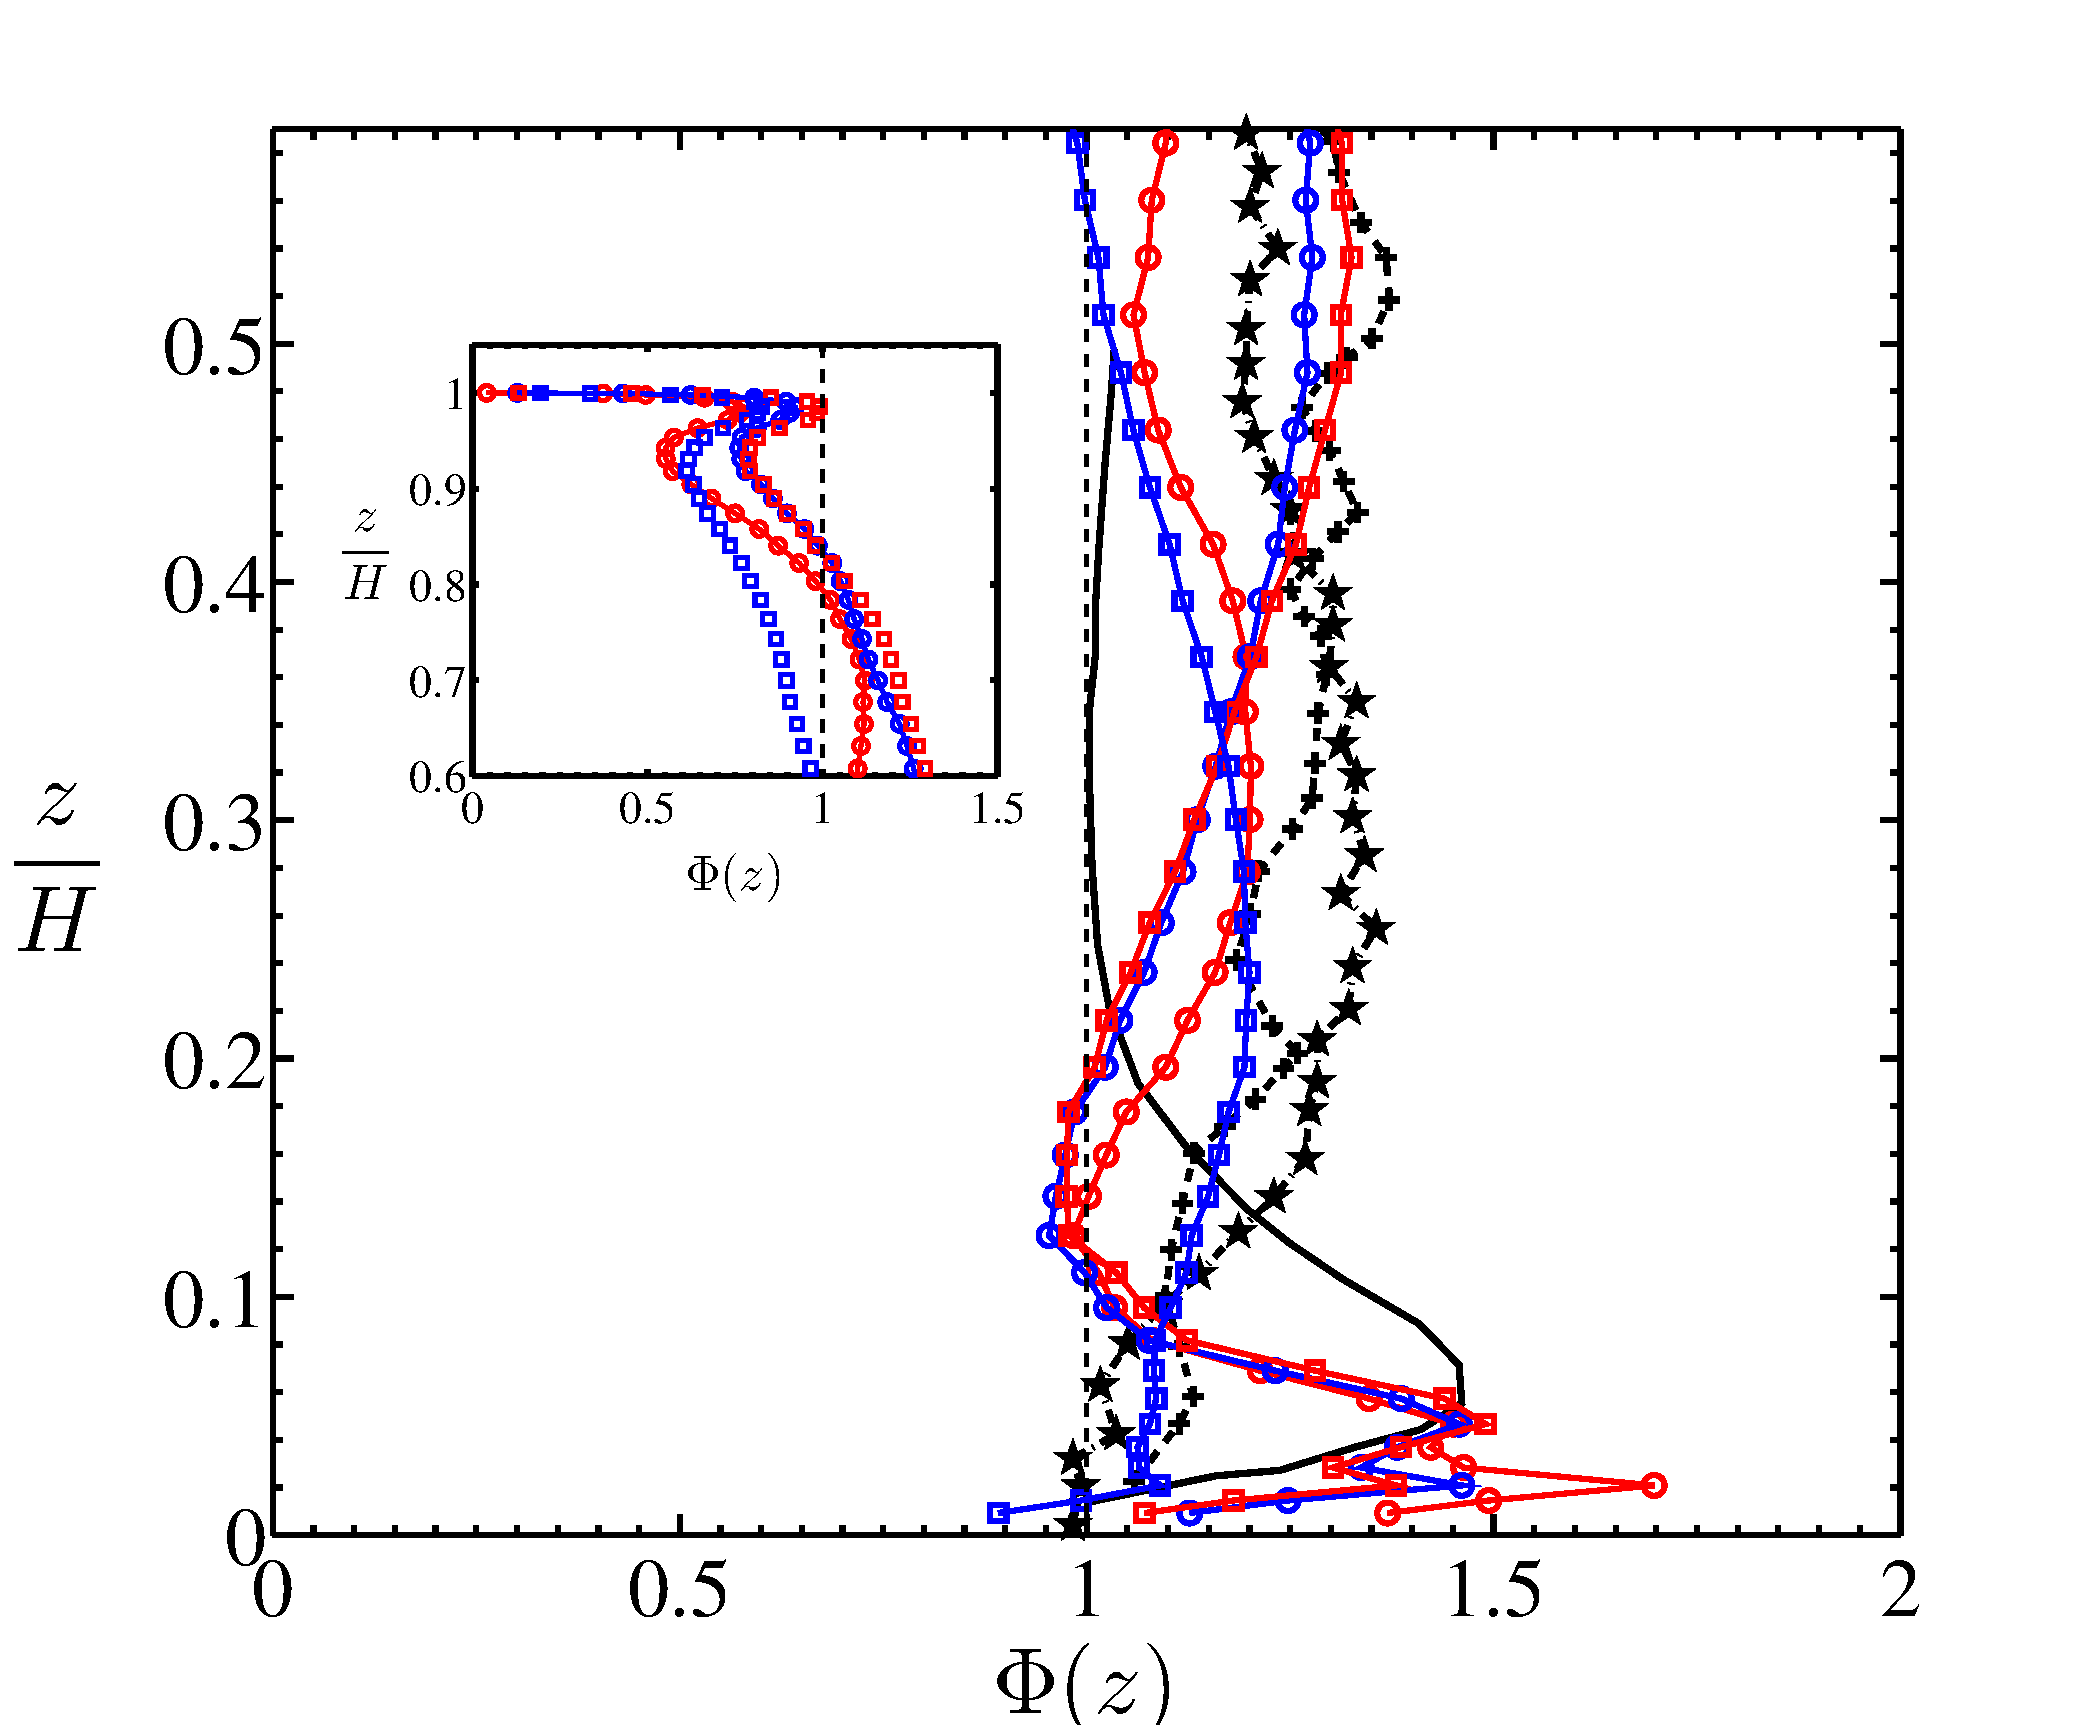
\includegraphics[width=\linewidth]{Fig2/gradient_filt_lotw.pdf}
                \caption{}
                \label{fig:grad1}
        \end{subfigure}%
        \centering
        \begin{subfigure}[t]{0.5\textwidth}
                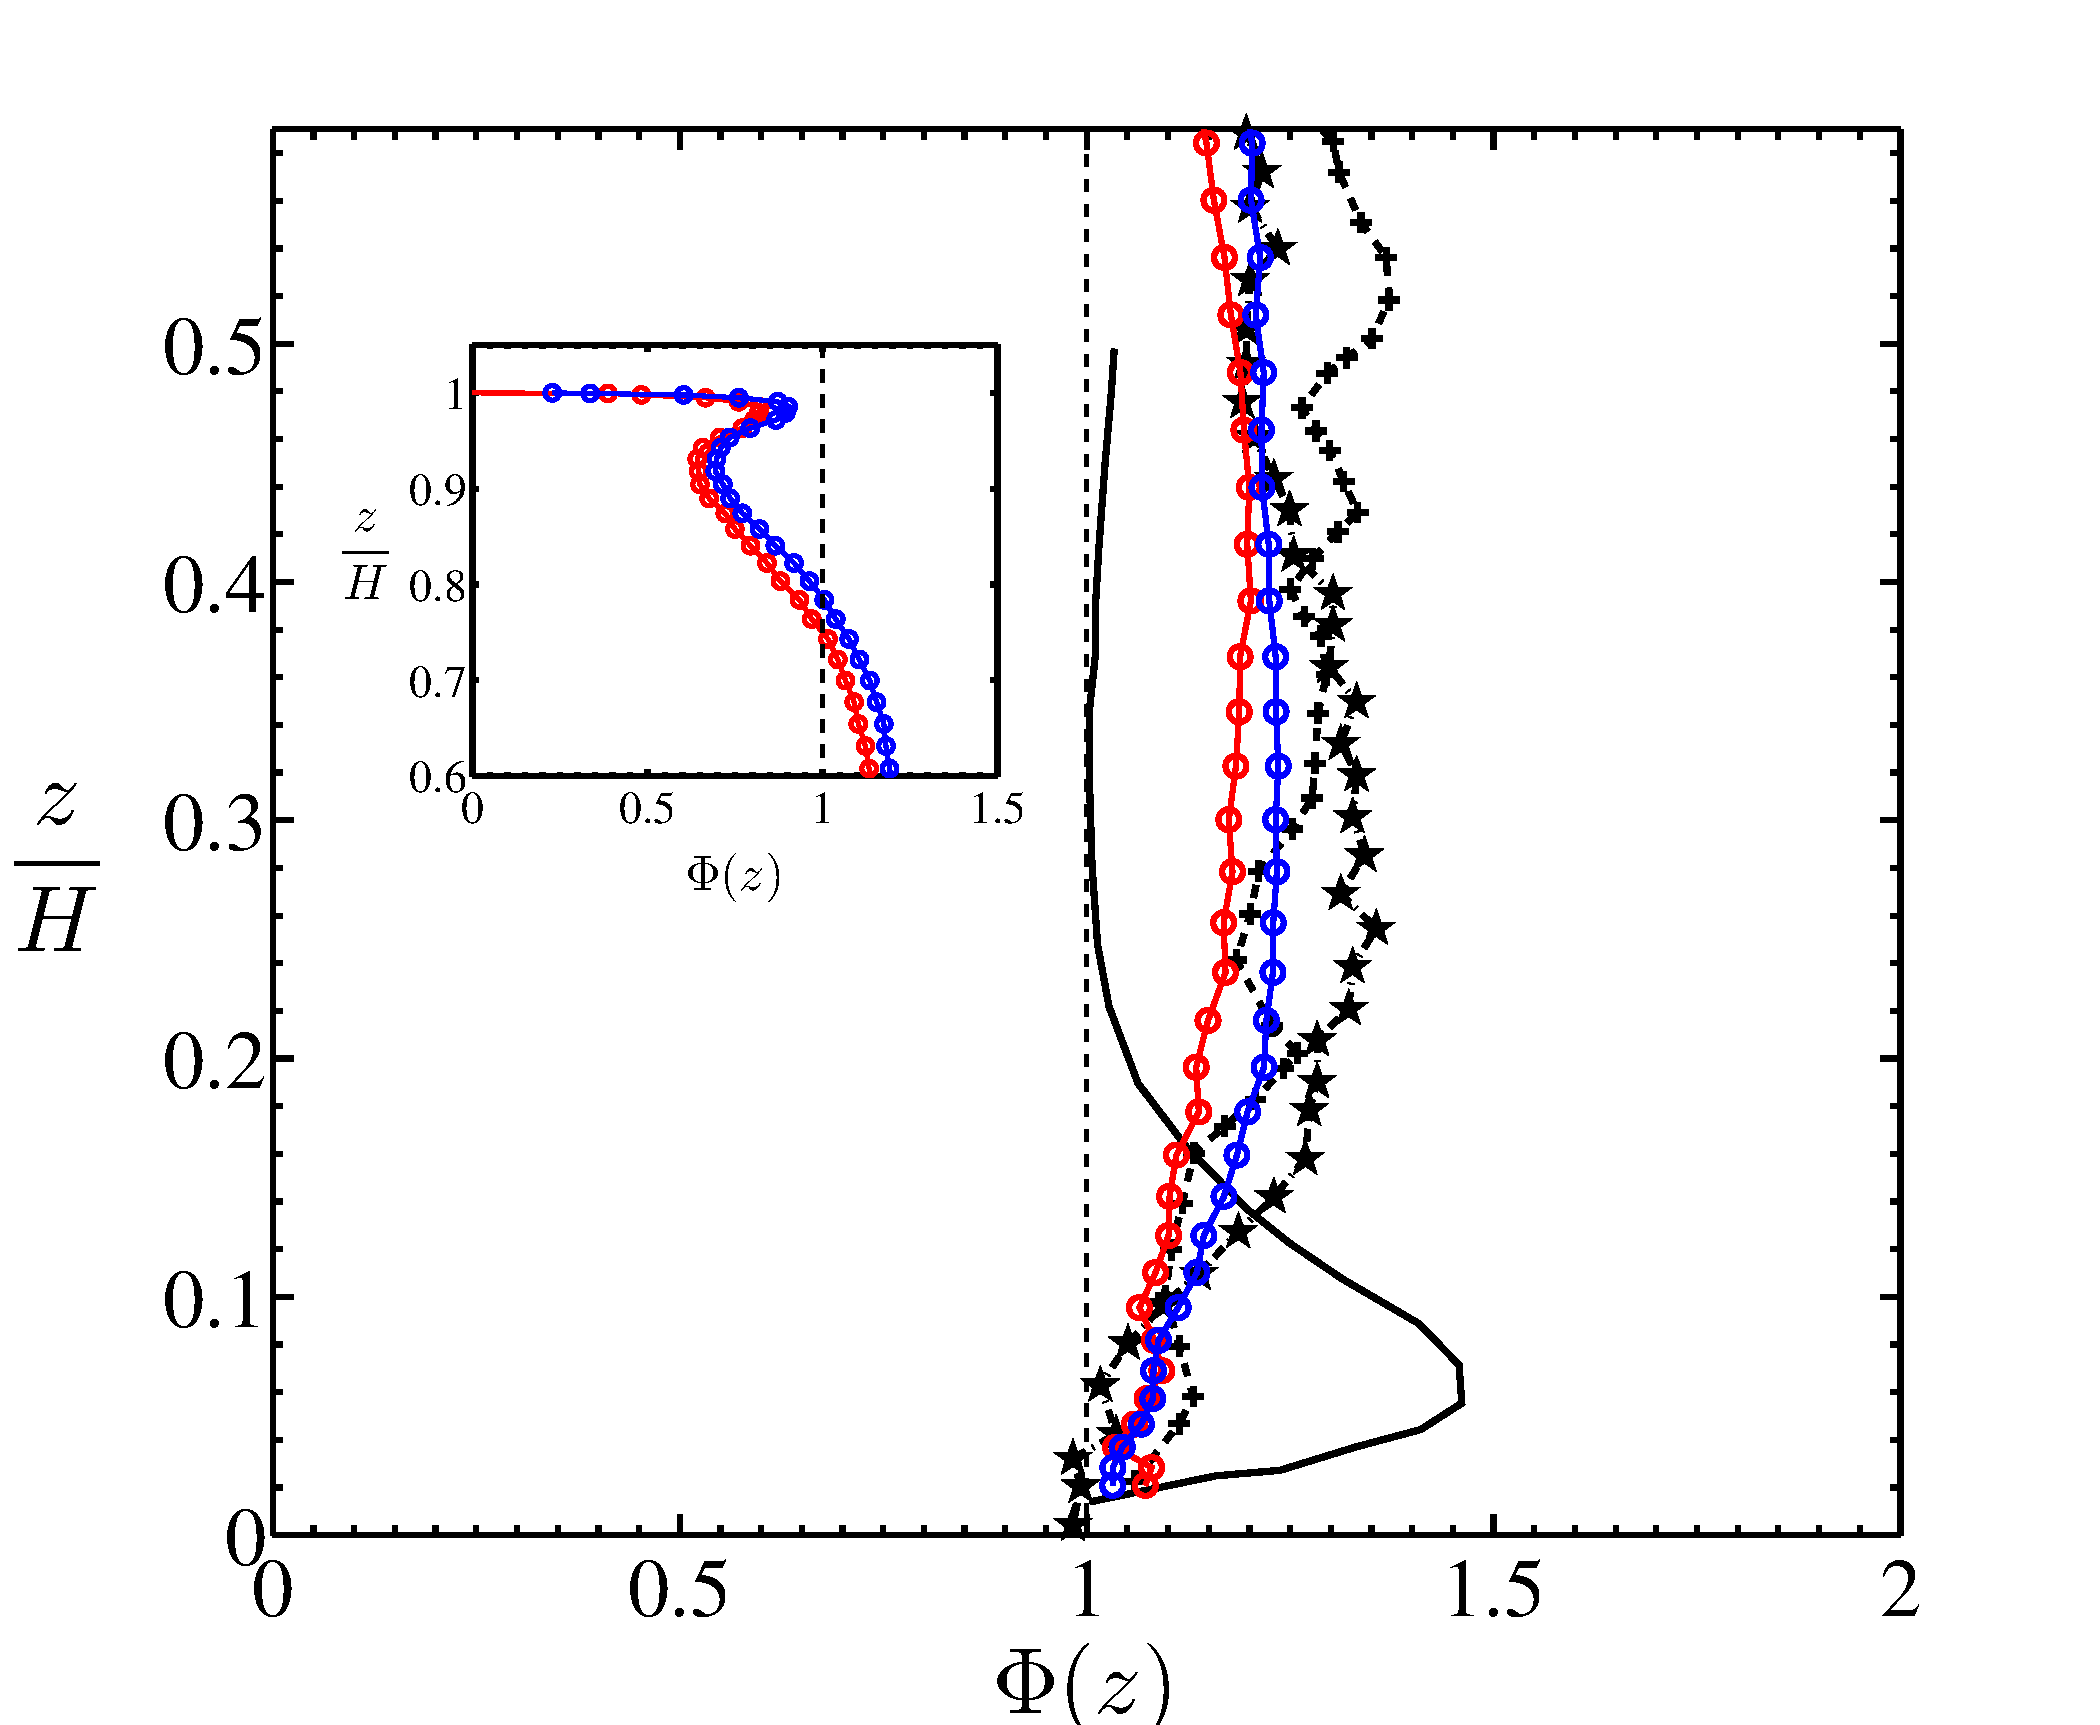
\includegraphics[width=\linewidth]{Fig2/gradient_filt_lotw2.pdf}
                \caption{}
                \label{fig:grad2}
        \end{subfigure}%
        \caption[$\Phi(z)$: interpolation, $C_0$]{Non dimensinonal mean streamwise velocity gradient $\phi(z)$ vs $z/H$. Red, Blue curves: current simulations; Black curves from the literature~\cite{porte1fun,bou1}. (a) $k_{c}=2$: Red $\circ$ $n = 1$; Blue $\circ$, $n = 2$; Red $\Box$, $n = 3$; Blue $\Box$, $C_0 = 0.13, n = \frac{1}{2}$.  (b) $k_c = 4$, $\lbrace C_0, \ n\rbrace = (0.19, 0.5)$: Red $\circ$ , spectral interpolation; Blue $\circ$ mid point interpolation. Black $+$ scale dependant dynamic Smagorinsky for Port$\acute{e}$-Agel et al.~\cite{porte1fun}; $-$ , standard Smagorinsky, $\star$, Lagrangian scale dependant dynamic Smagorinsky with filtering, Bou-Zeid et. al~\cite{bou1}}\label{fig:stat0_lotw}
\end{figure}

\begin{figure}
        \centering
        \begin{subfigure}[t]{0.55\textwidth}
                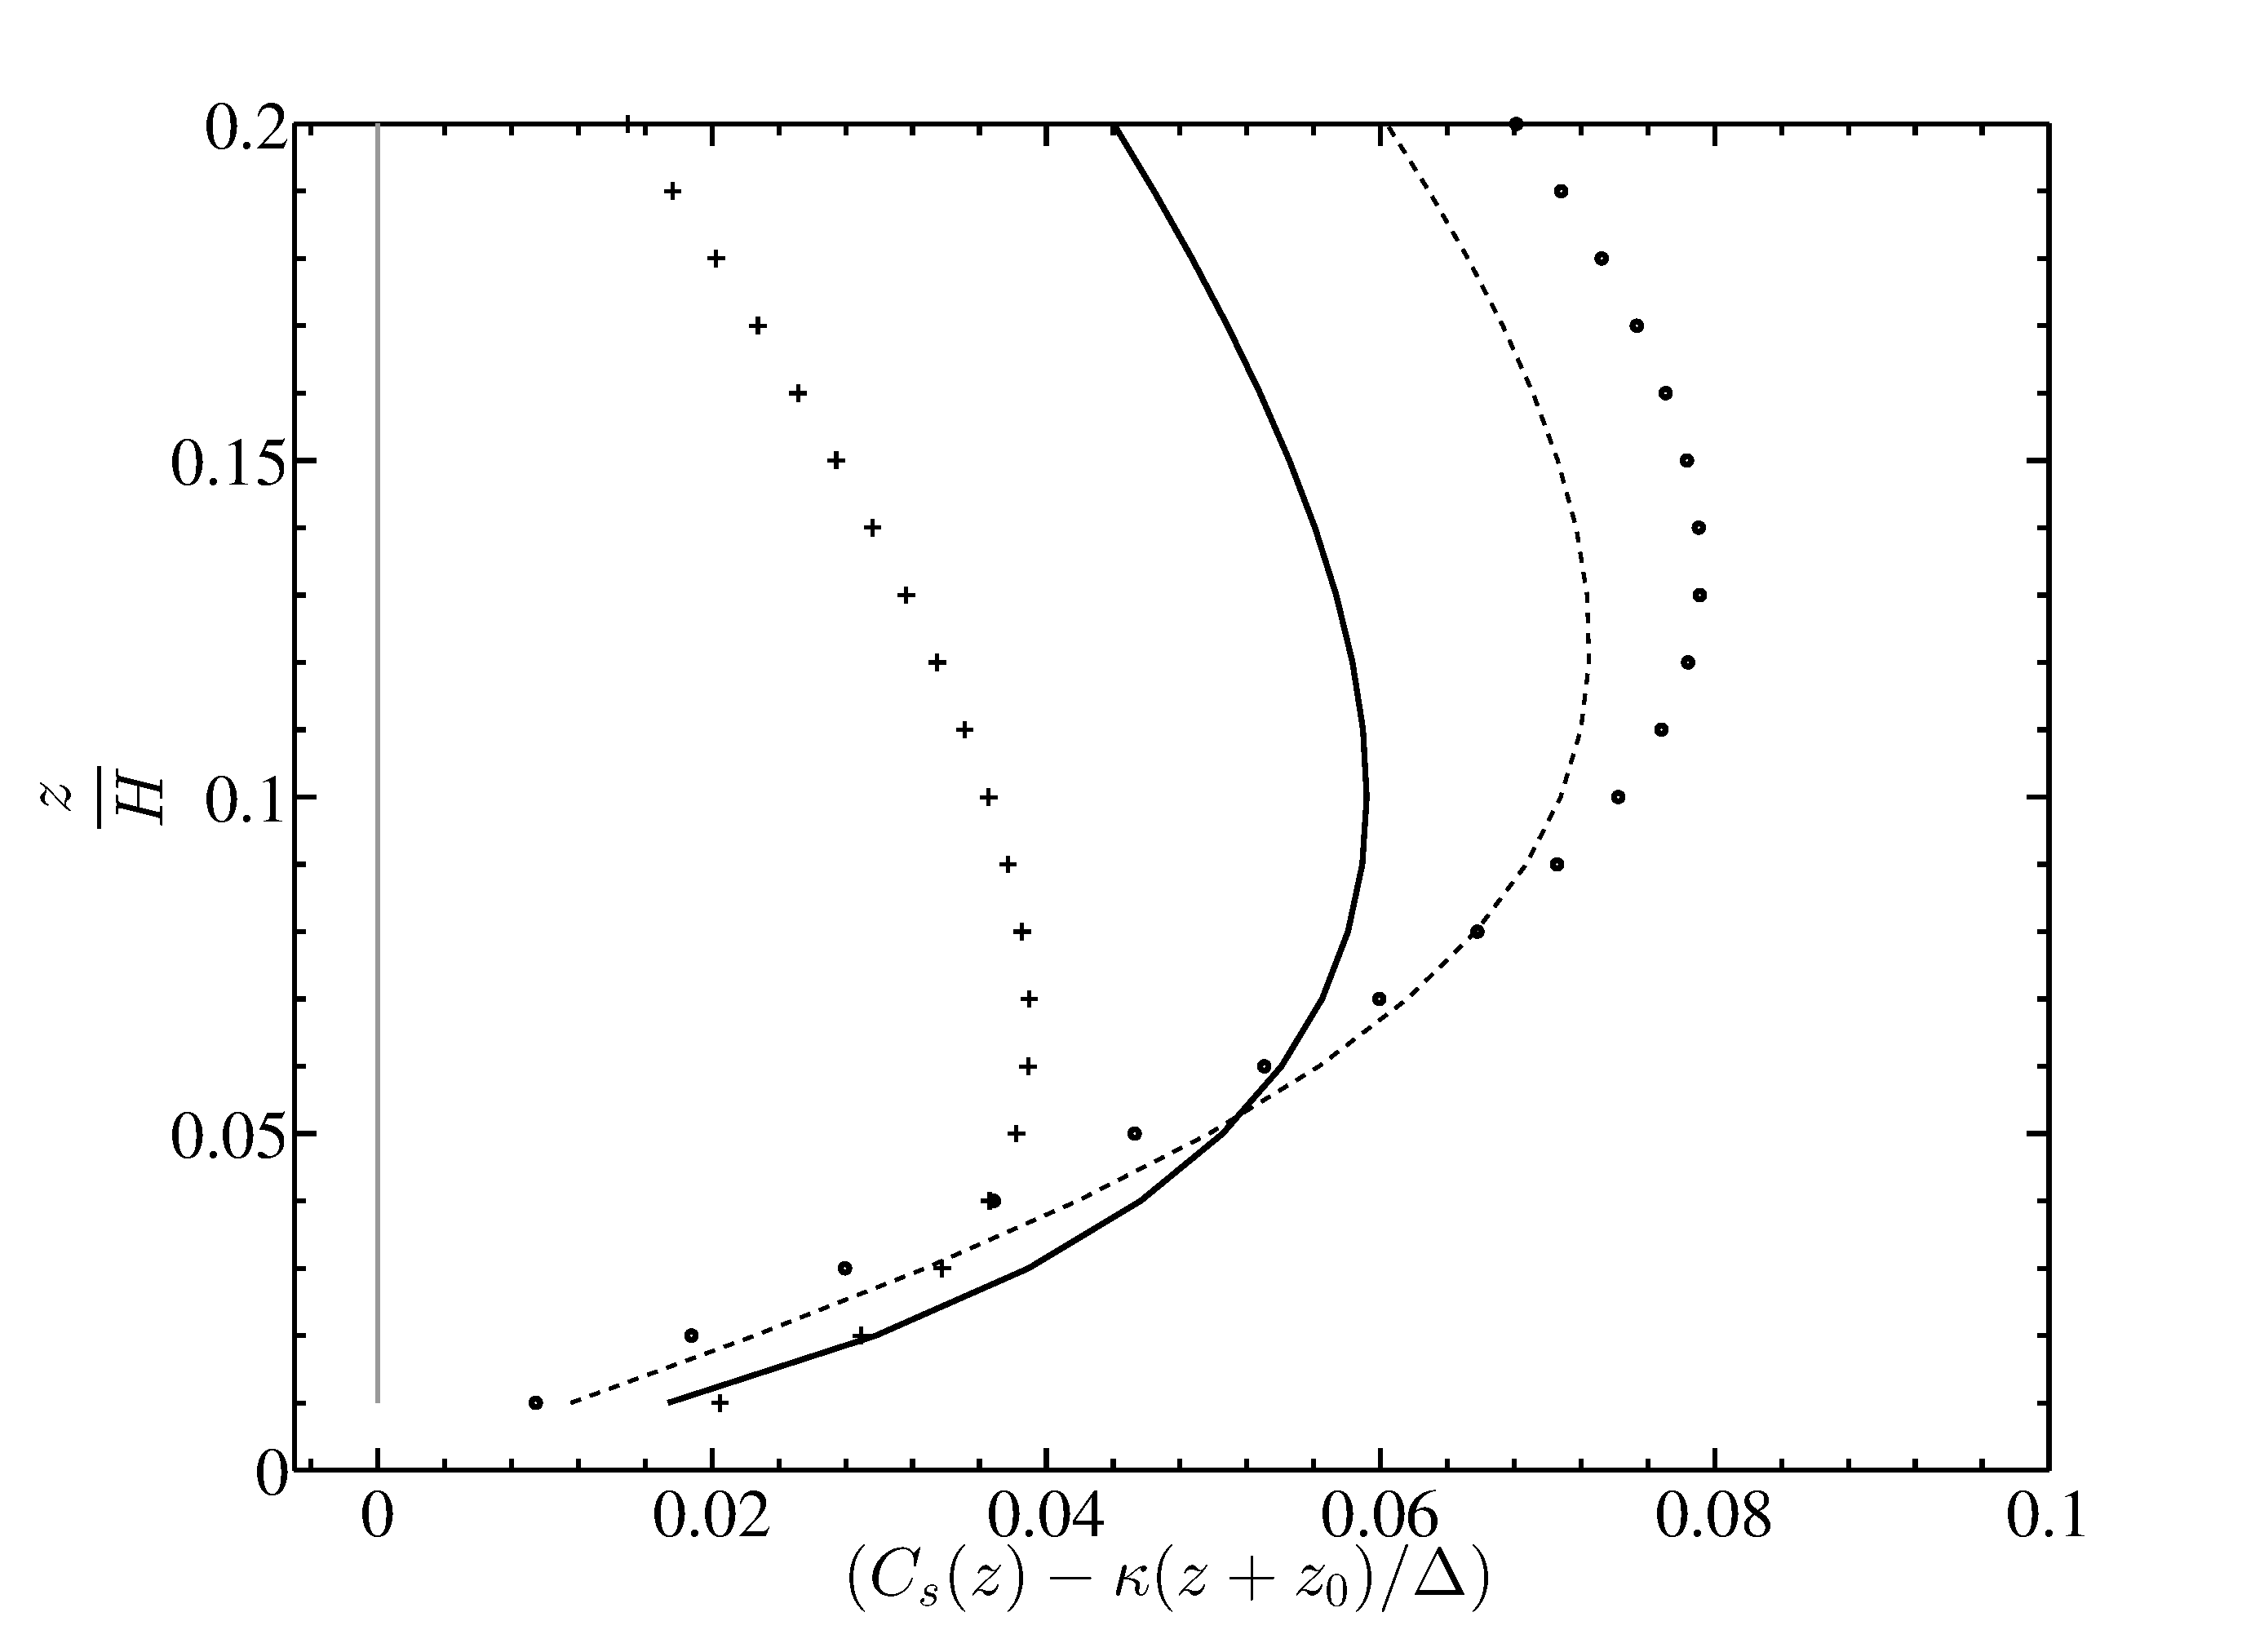
\includegraphics[width=\linewidth]{Fig2/Smag2b_abs.pdf}
                \caption{}
                \label{fig:error1}
        \end{subfigure}%
        \centering
        \begin{subfigure}[t]{0.45\textwidth}
                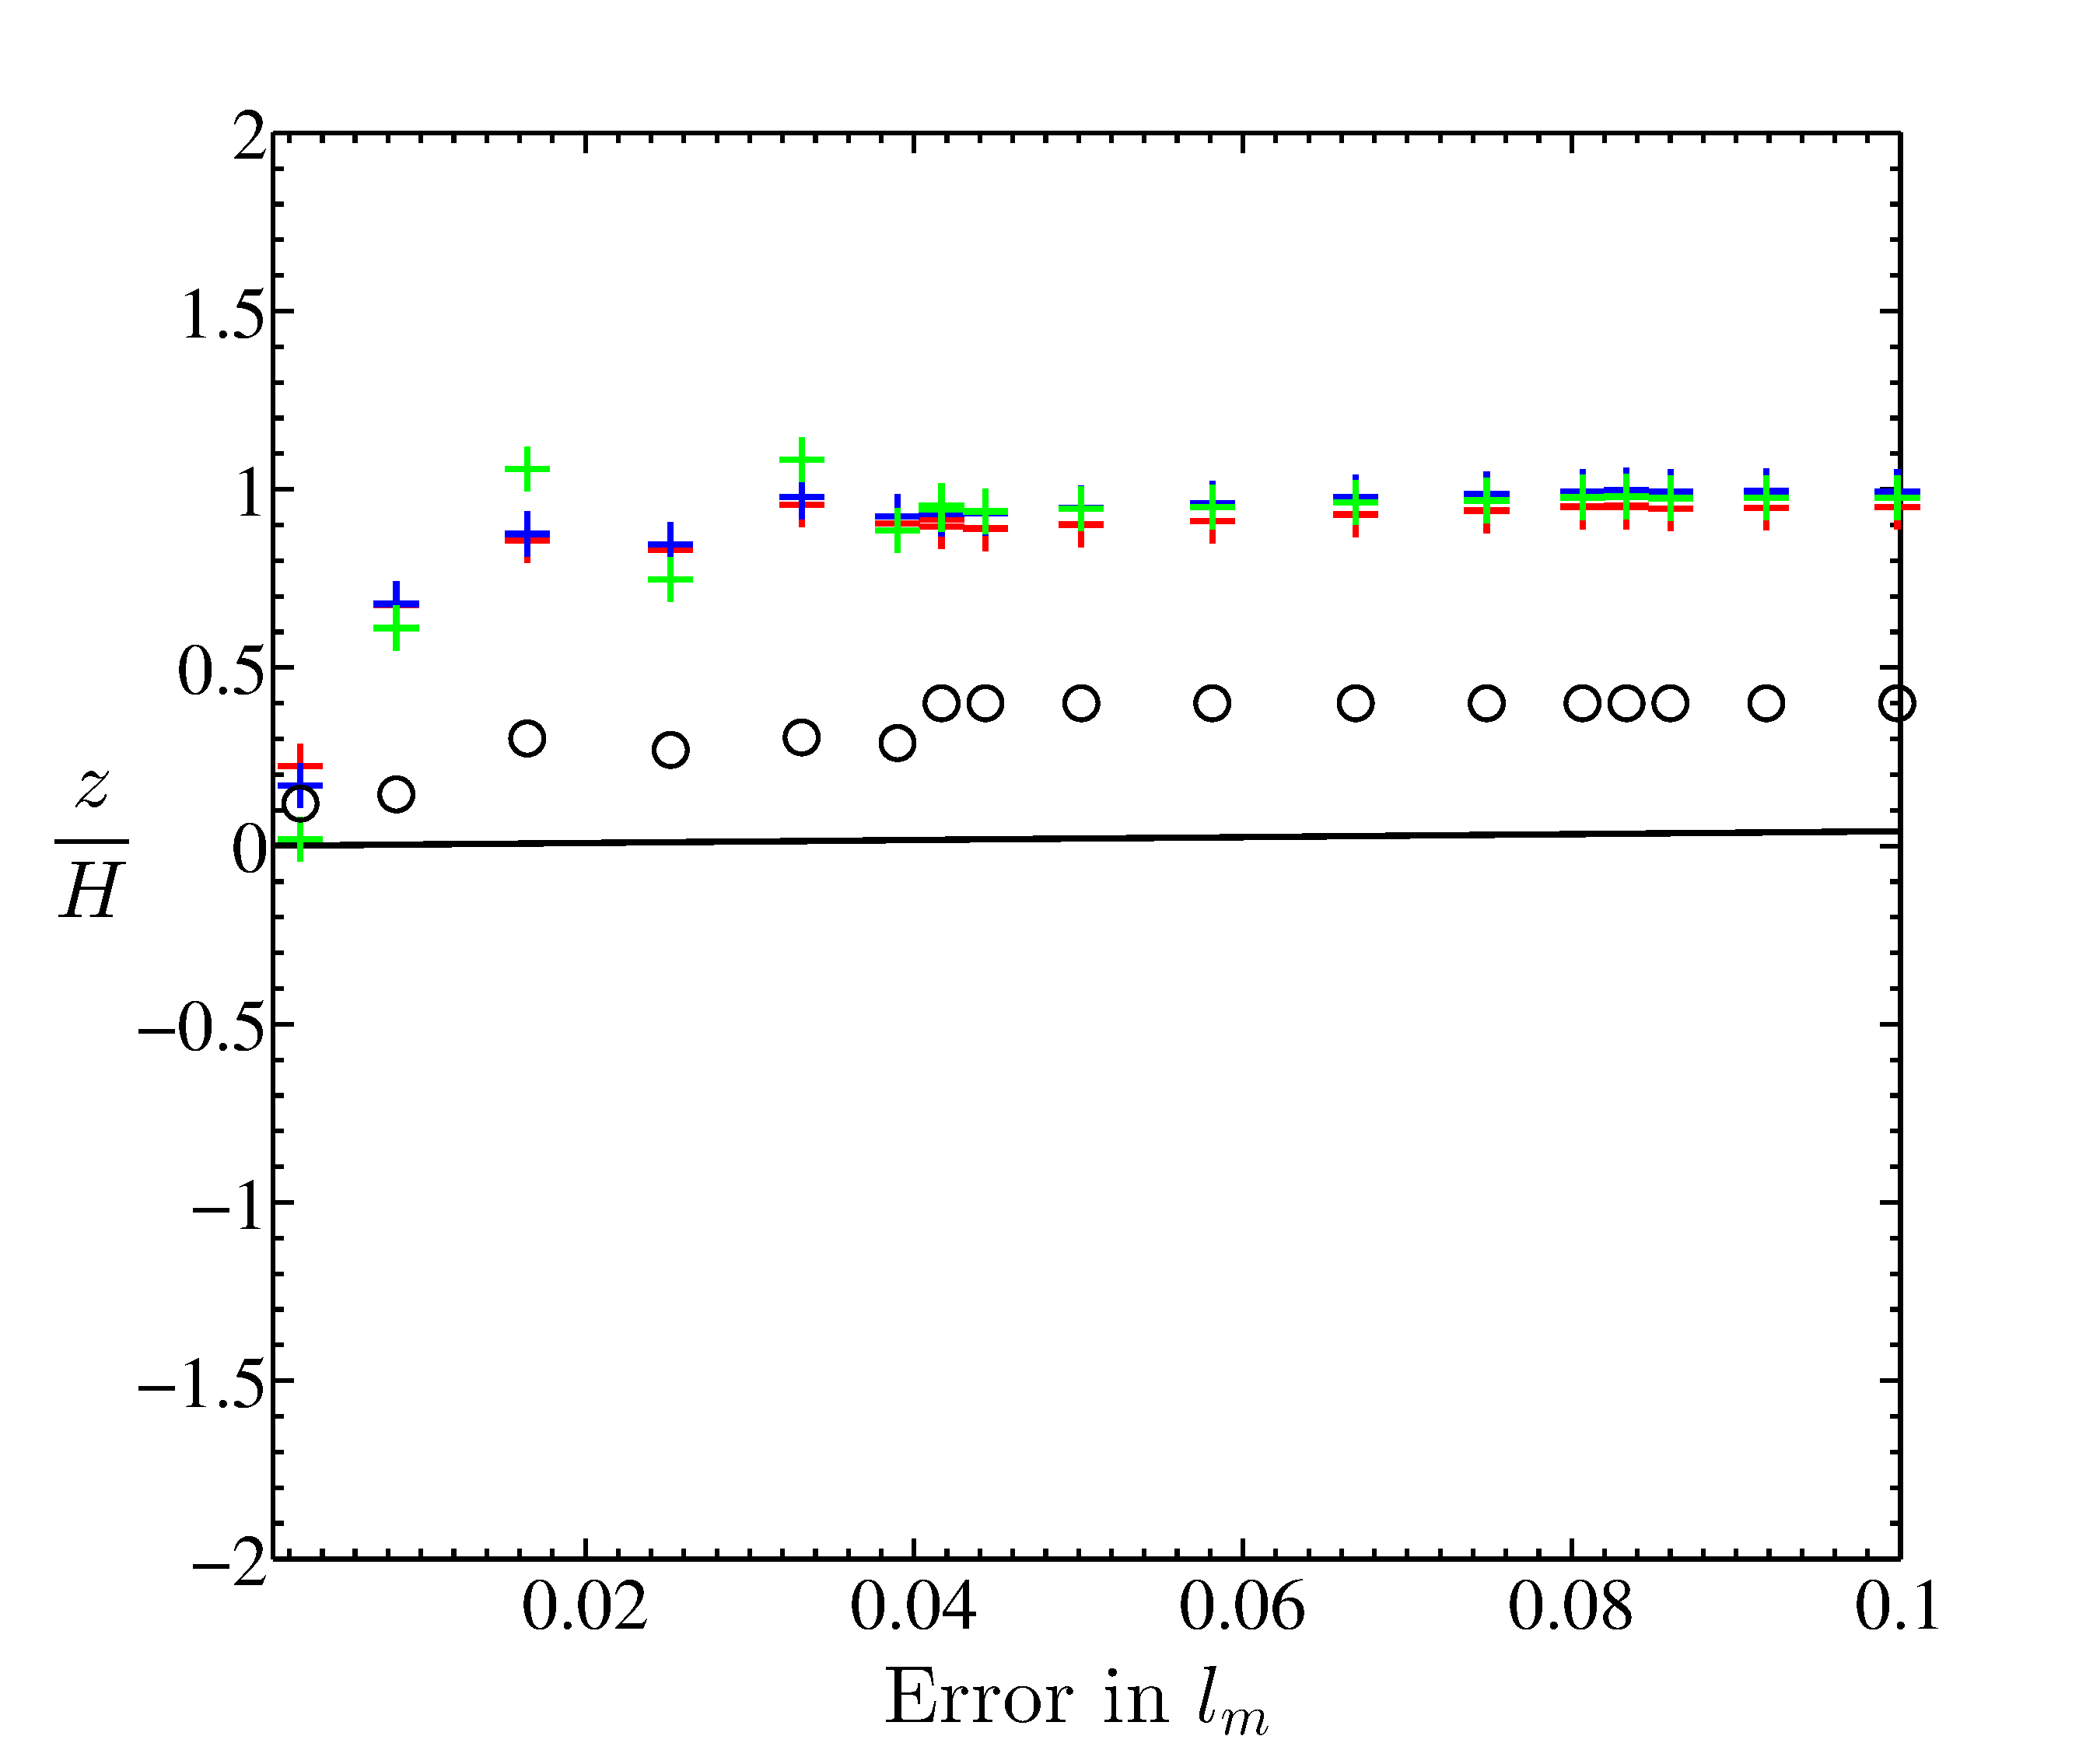
\includegraphics[width=\linewidth]{Fig2/shear_filter_n123.pdf}
                \caption{}
                \label{fig:error2}
        \end{subfigure}
\caption[Errors contributing in log-layer mismatch]{(a)Error $E_{1}$ in filter-scale $l_f$ compared to mixing length scale at log-layer $\kappa z$. (b) Error $E2$ in eddy-turnover time length scale $u_{\tau} \times t_{eddy}$ compared to log-layer mixing-length scale $\kappa z$. solid Black line: $\kappa z$. Symbols: Red, Blue $\&$ Green $+$, corresponds to $(n = 1, C_0 = 0.17, k_c = 4)$, $(n = 1, C_0 = 0.17,k_c = 2)$, $(n = 1, C_0 = 0.13, k_c = 4)$ respectively. Black $\circ$, $(n = \frac{1}{2}, C_0 = 0.19, k_c = 4)$. $E_1$ is the modelling error, $E_2$ is the numerical error.}
                \label{fig:shear1}
\end{figure}

\begin{figure}[h!]
        \centering
        \begin{subfigure}[t]{0.70\textwidth}
                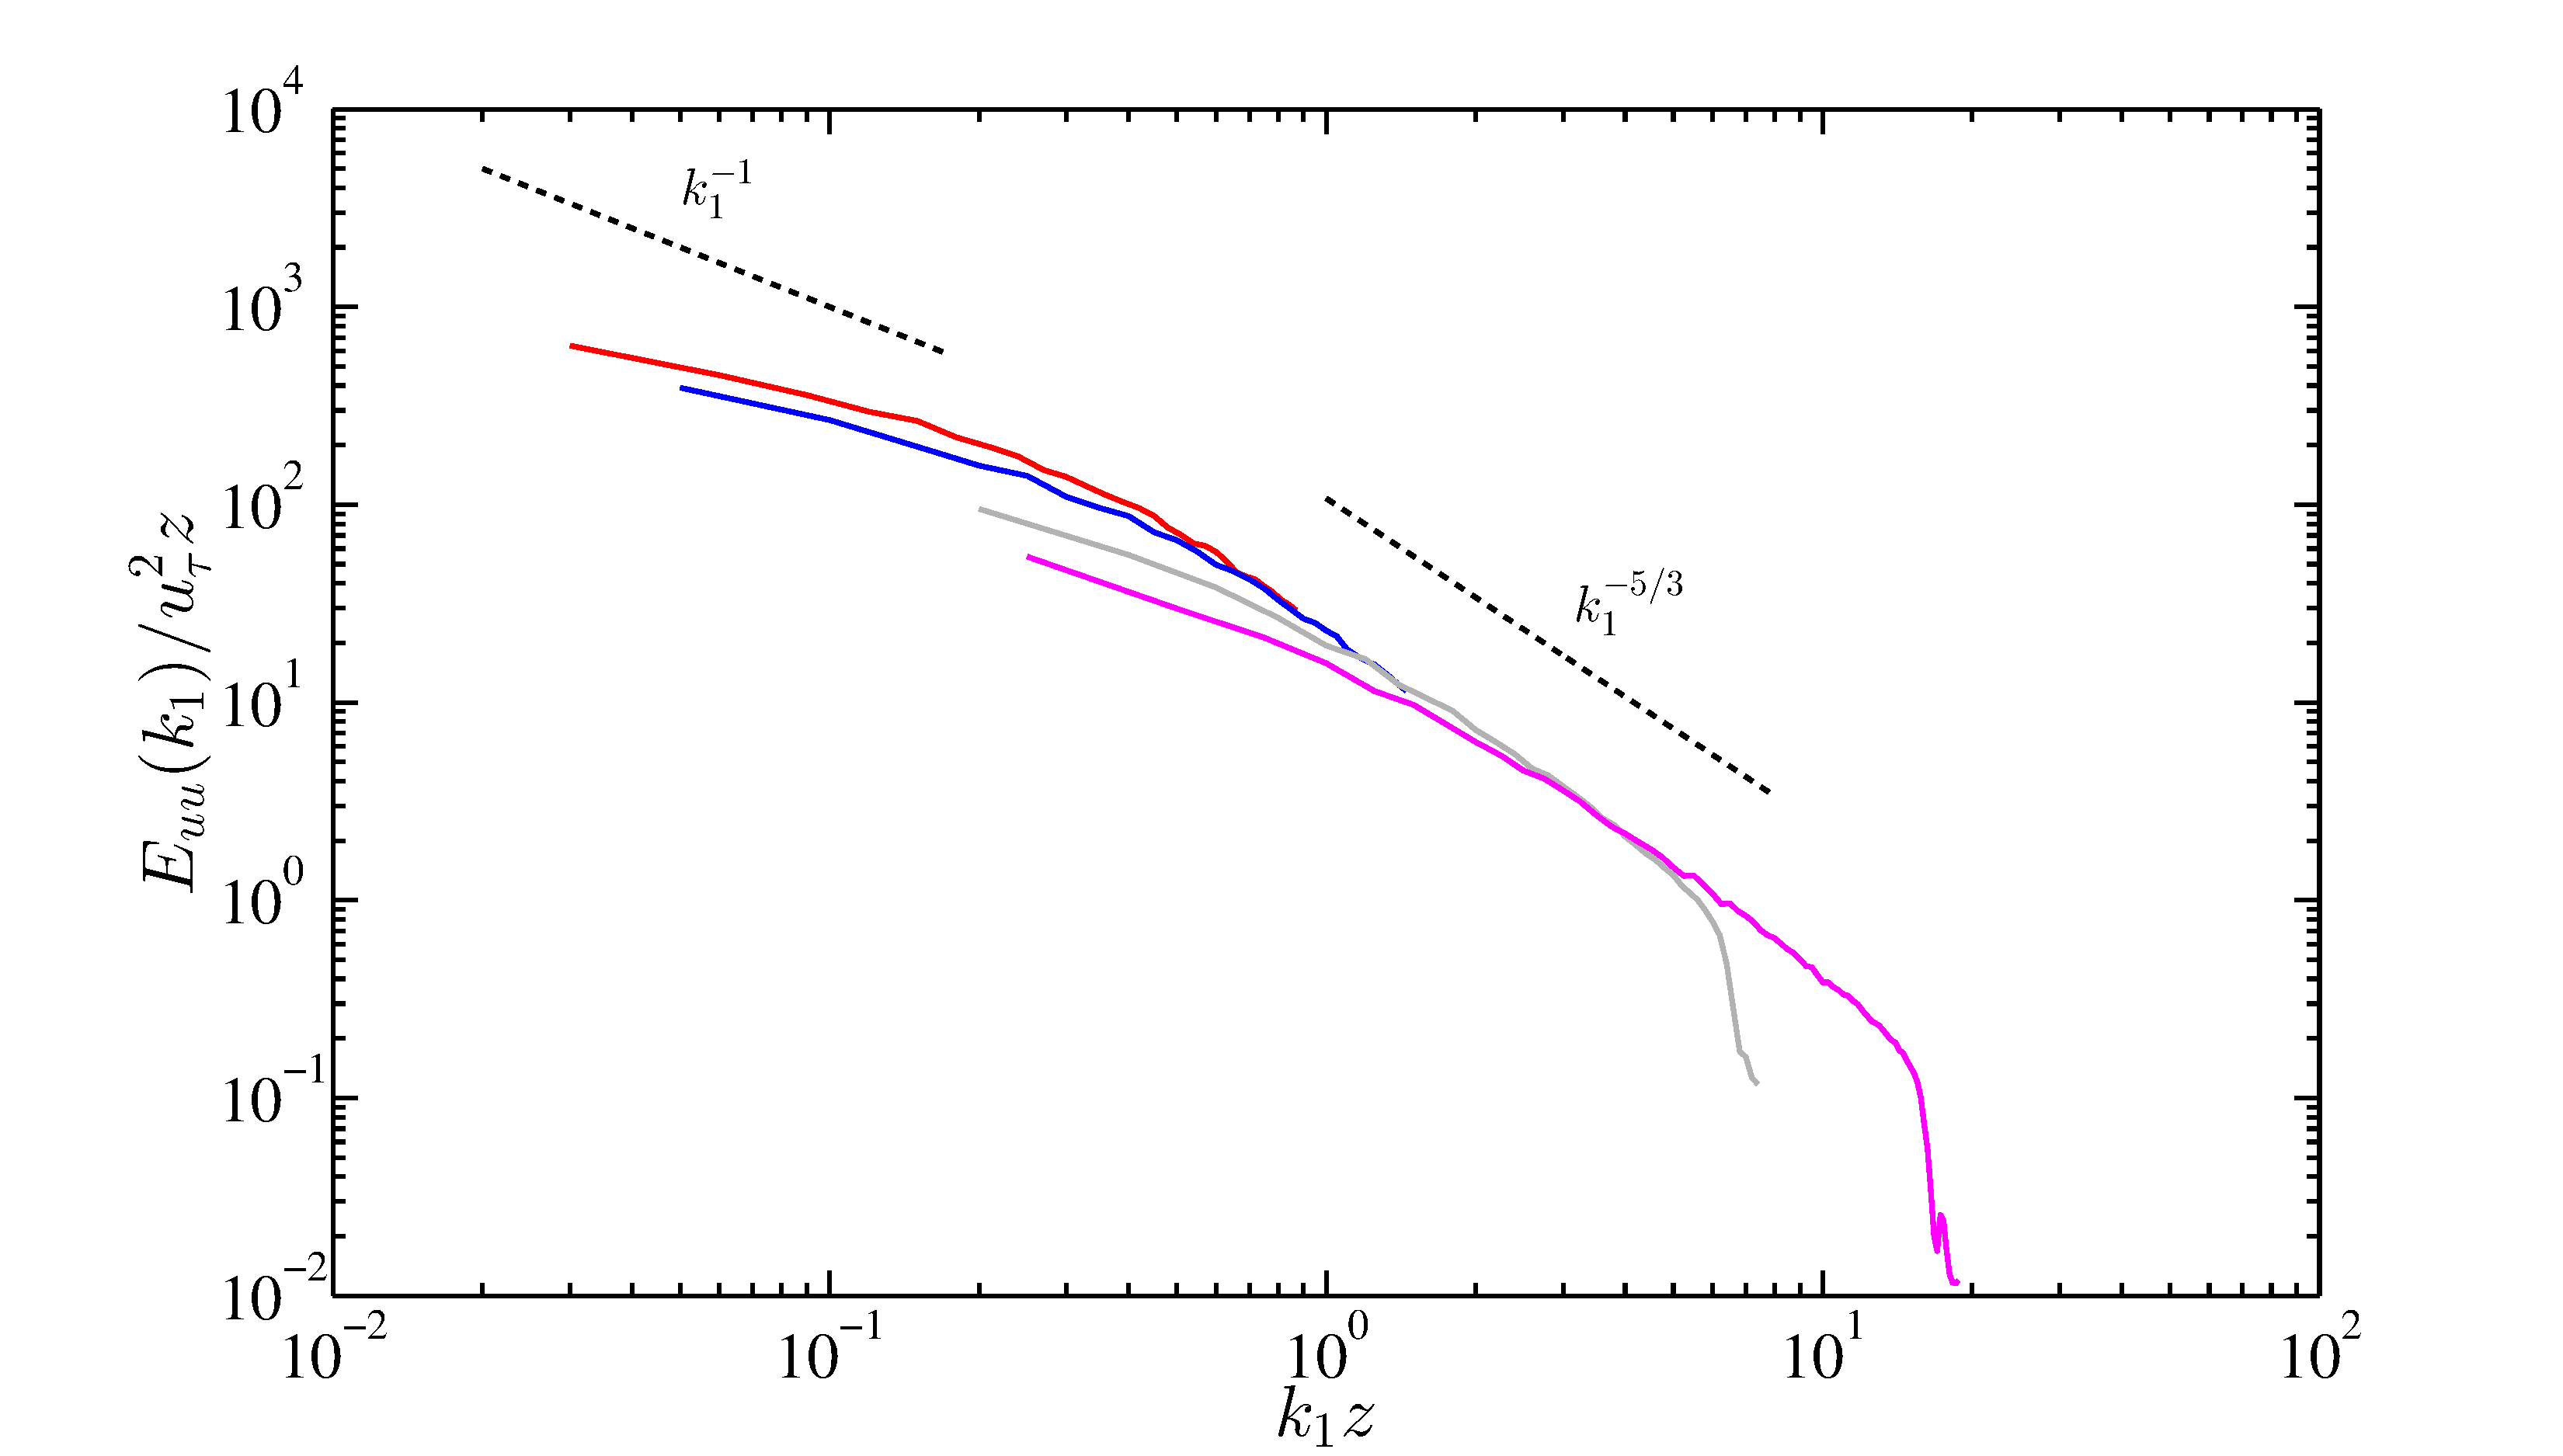
\includegraphics[width=\linewidth]{Fig2/energy_ABL_n05_filt2.pdf}
                \caption{}
                \label{fig:spec}
        \end{subfigure}
\centering
        \begin{subfigure}[t]{0.70\textwidth}
                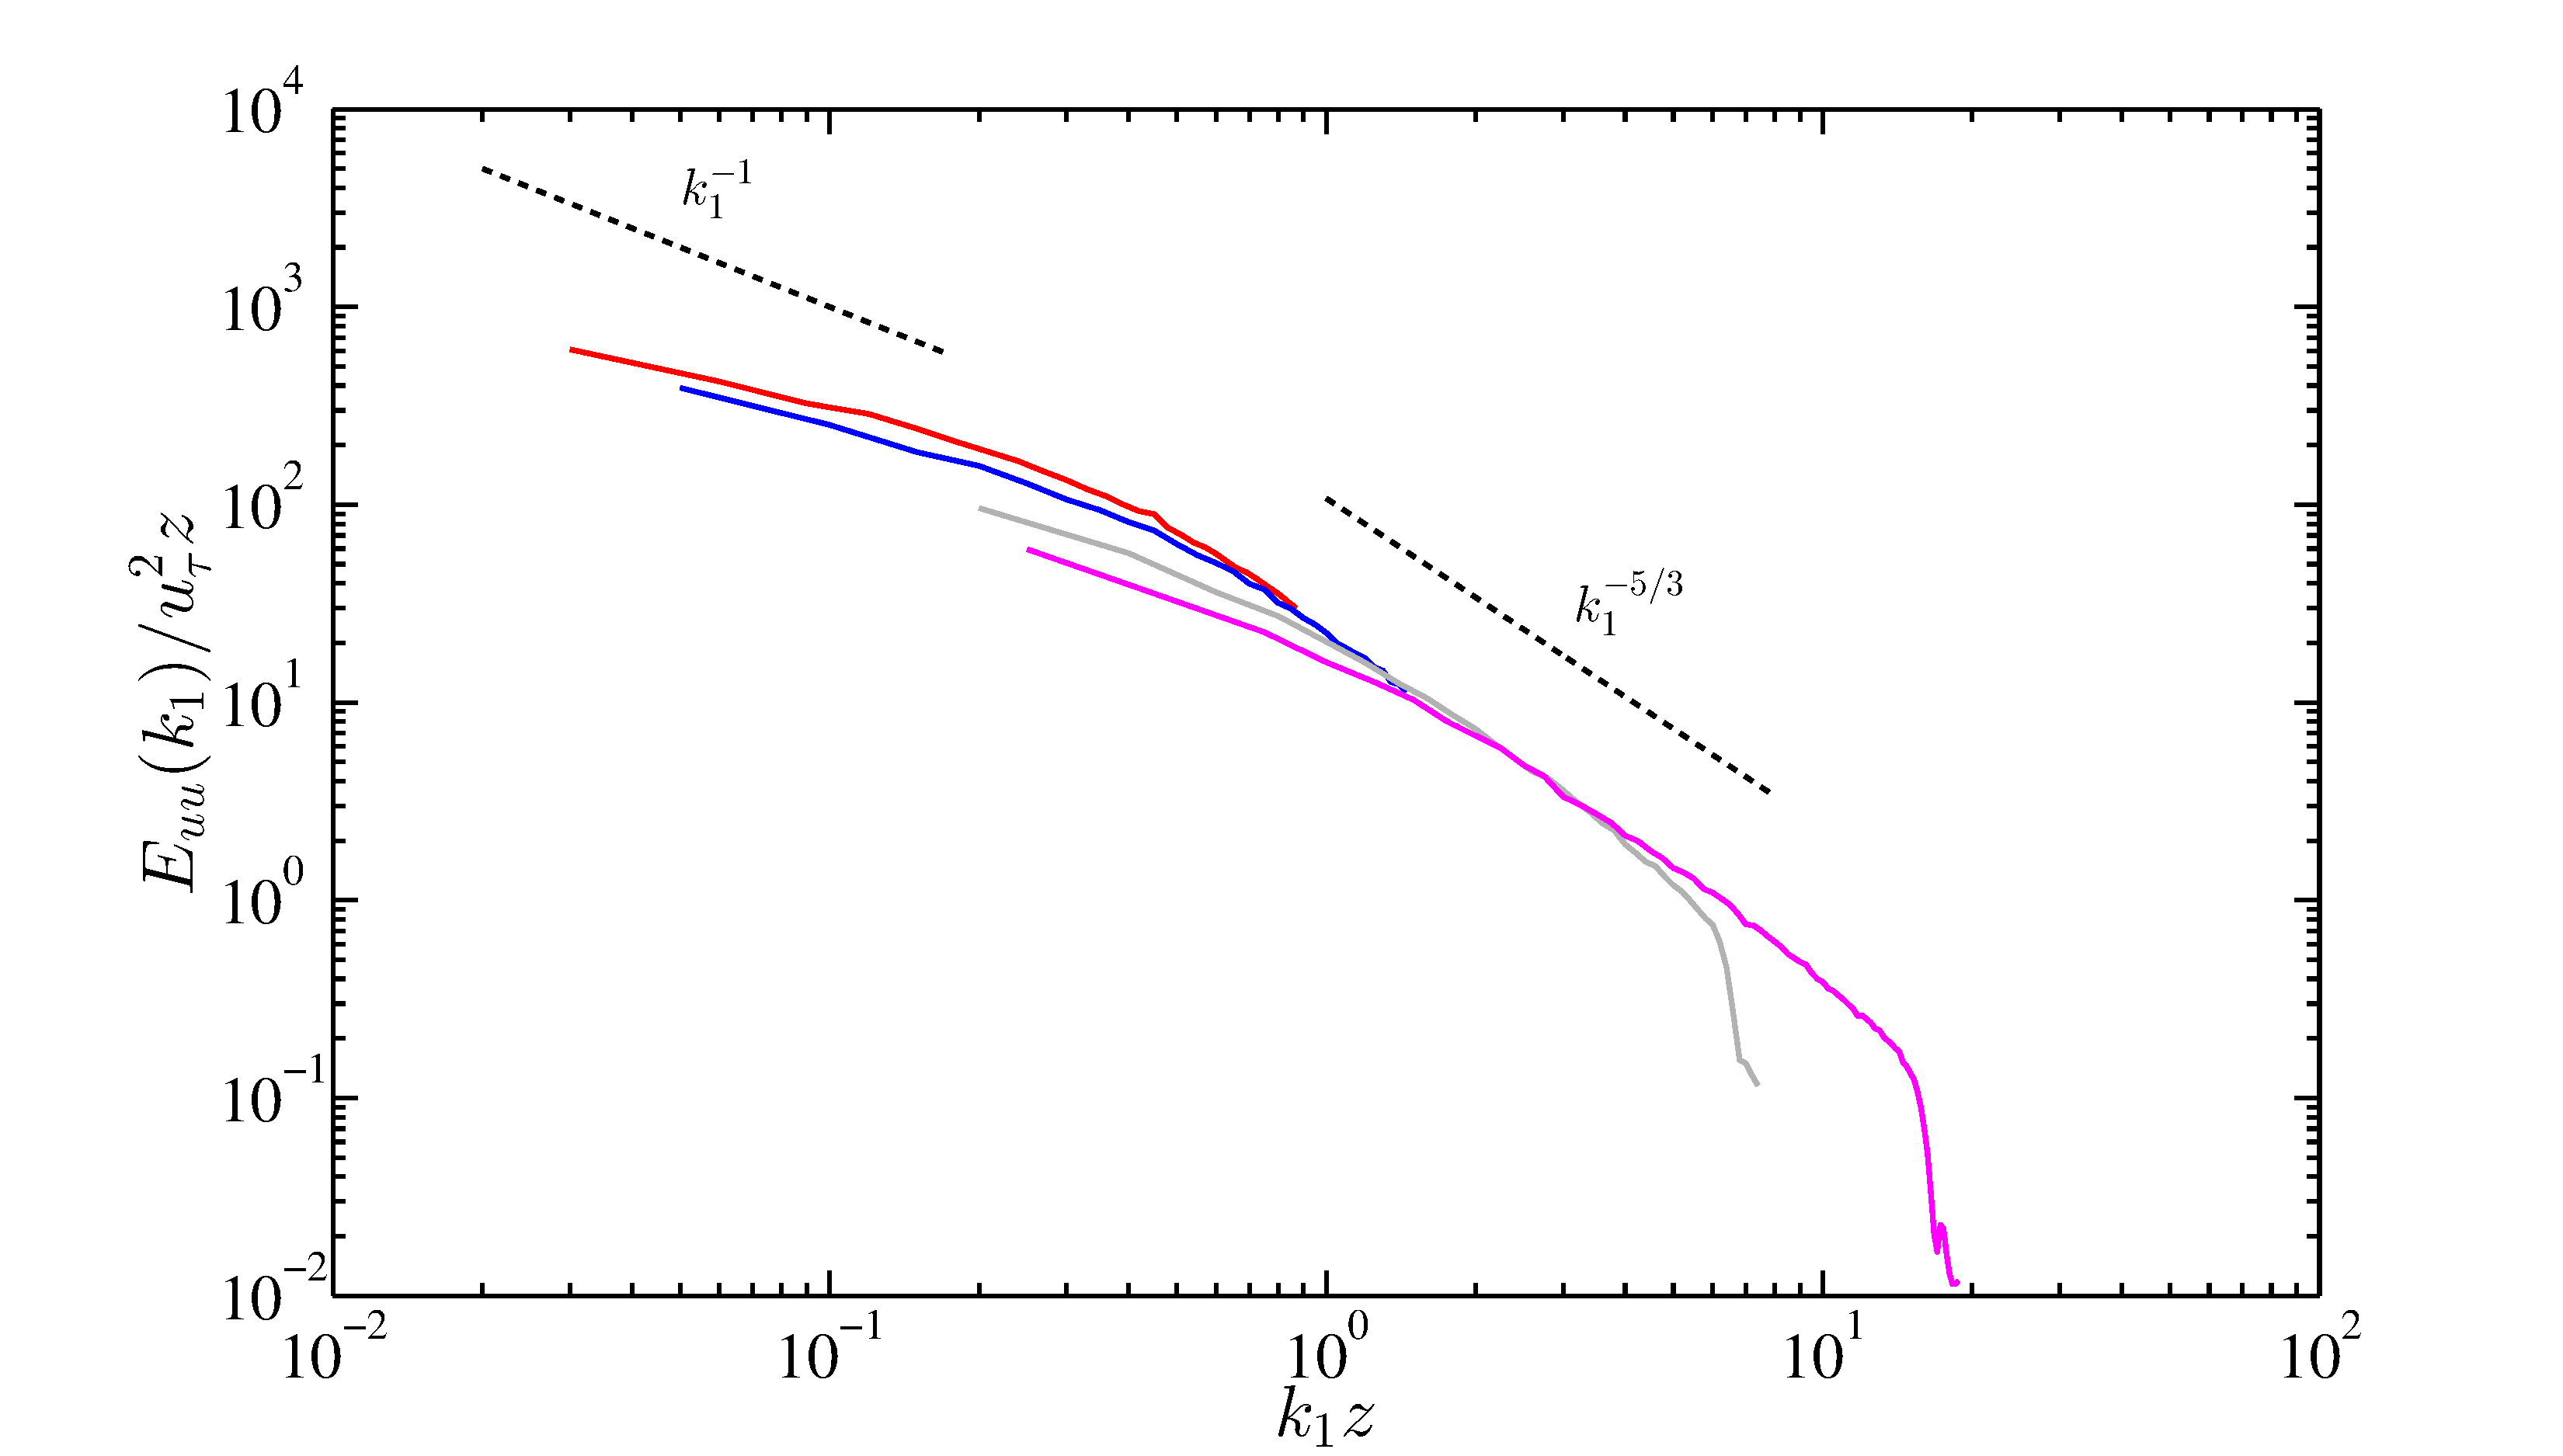
\includegraphics[width=\linewidth]{Fig2/energy_ABL_n05_filt4.pdf}
                \caption{}
                \label{fig:spec2}
        \end{subfigure}
\centering
        \begin{subfigure}[t]{0.70\textwidth}
                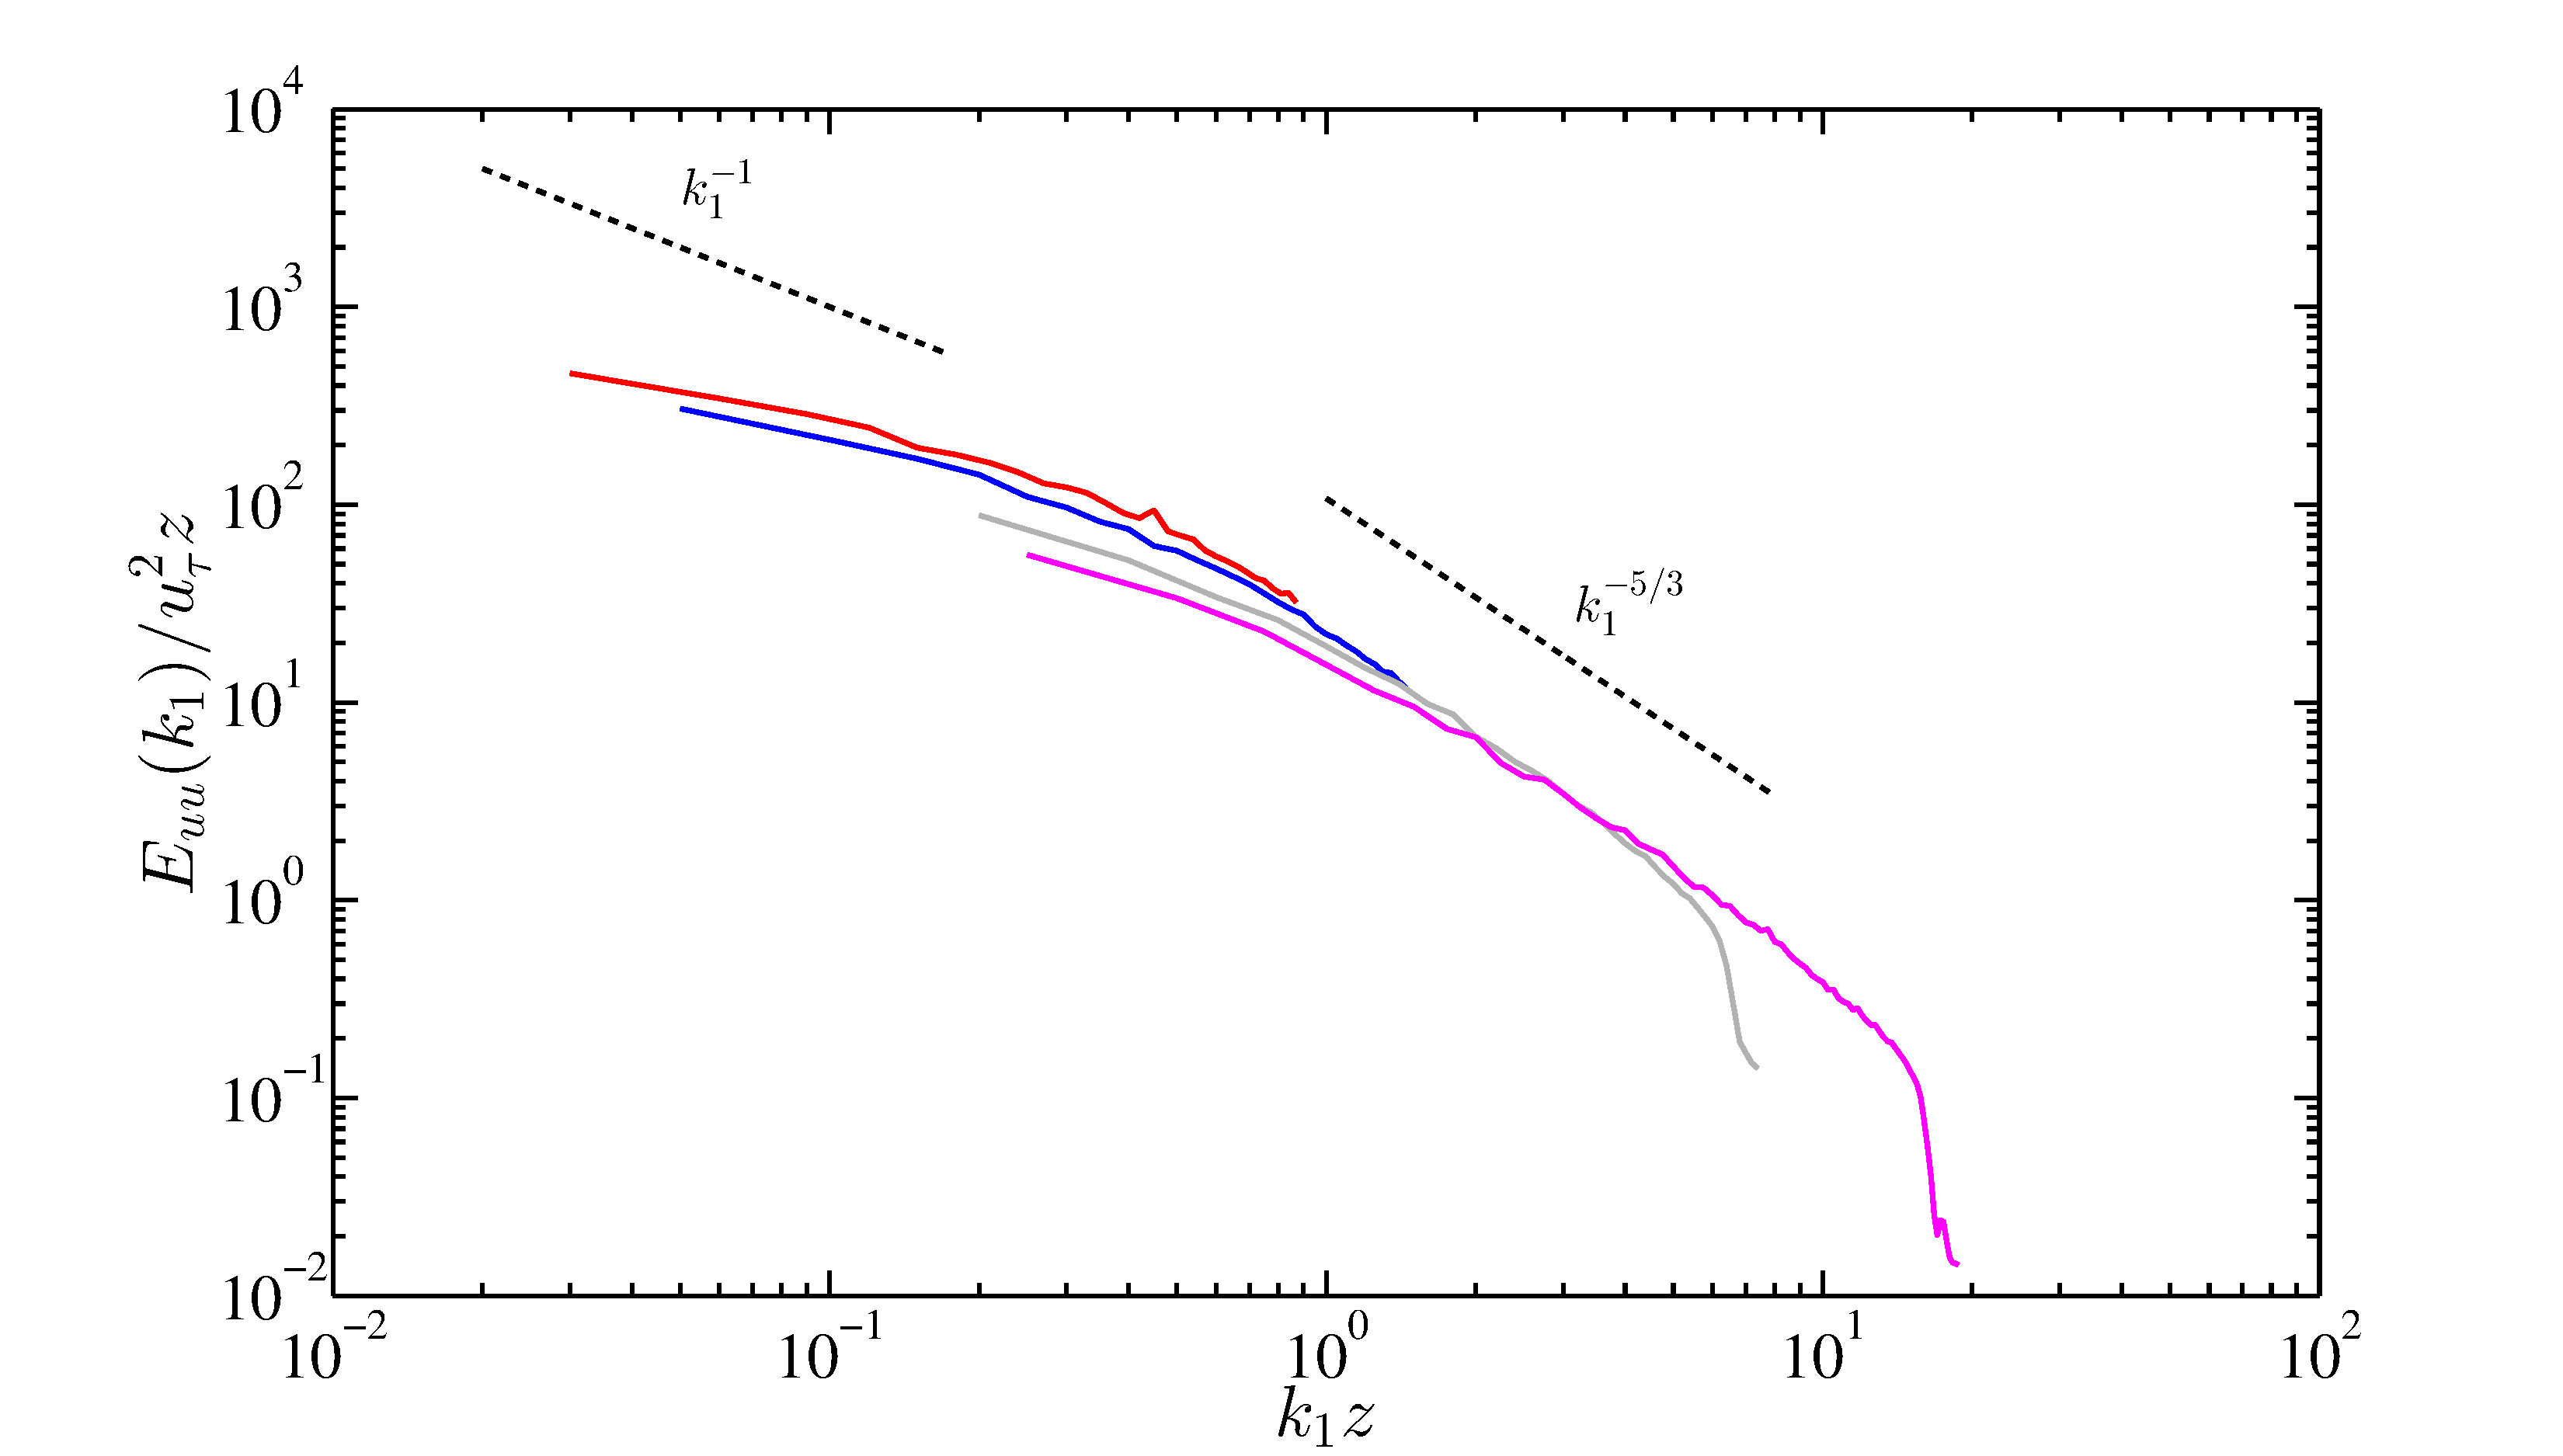
\includegraphics[width=\linewidth]{Fig2/energy_ABL_n05_filt6.pdf}
                \caption{}
                \label{fig:spec3}
        \end{subfigure}        
        \caption[1D Energy Spectra 1]{ Temporally and Horizontally averaged streamwise energy spectrum (A) Case VII, $k_c = 2$ (B) Case VIII, $k_c = 4$ (C) Case IX, $k_c = 6$. The Smagorinsky mixing length damping parameters $\lbrace C_0, \ n \rbrace = \lbrace 0.19, 0.5\rbrace$ are fixed, $k_c$ is varied. $k_1$ is the streamwise wavenumber. Red, $z/H = 0.015$, Blue, $z/H = 0.025$, Grey, $z/H = 0.1$, Magenta, $z/H = 0.25$ }\label{fig:stat0_lotw2}
\end{figure}
        
   \begin{figure}        
\centering
          \begin{subfigure}[t]{0.70\textwidth}
                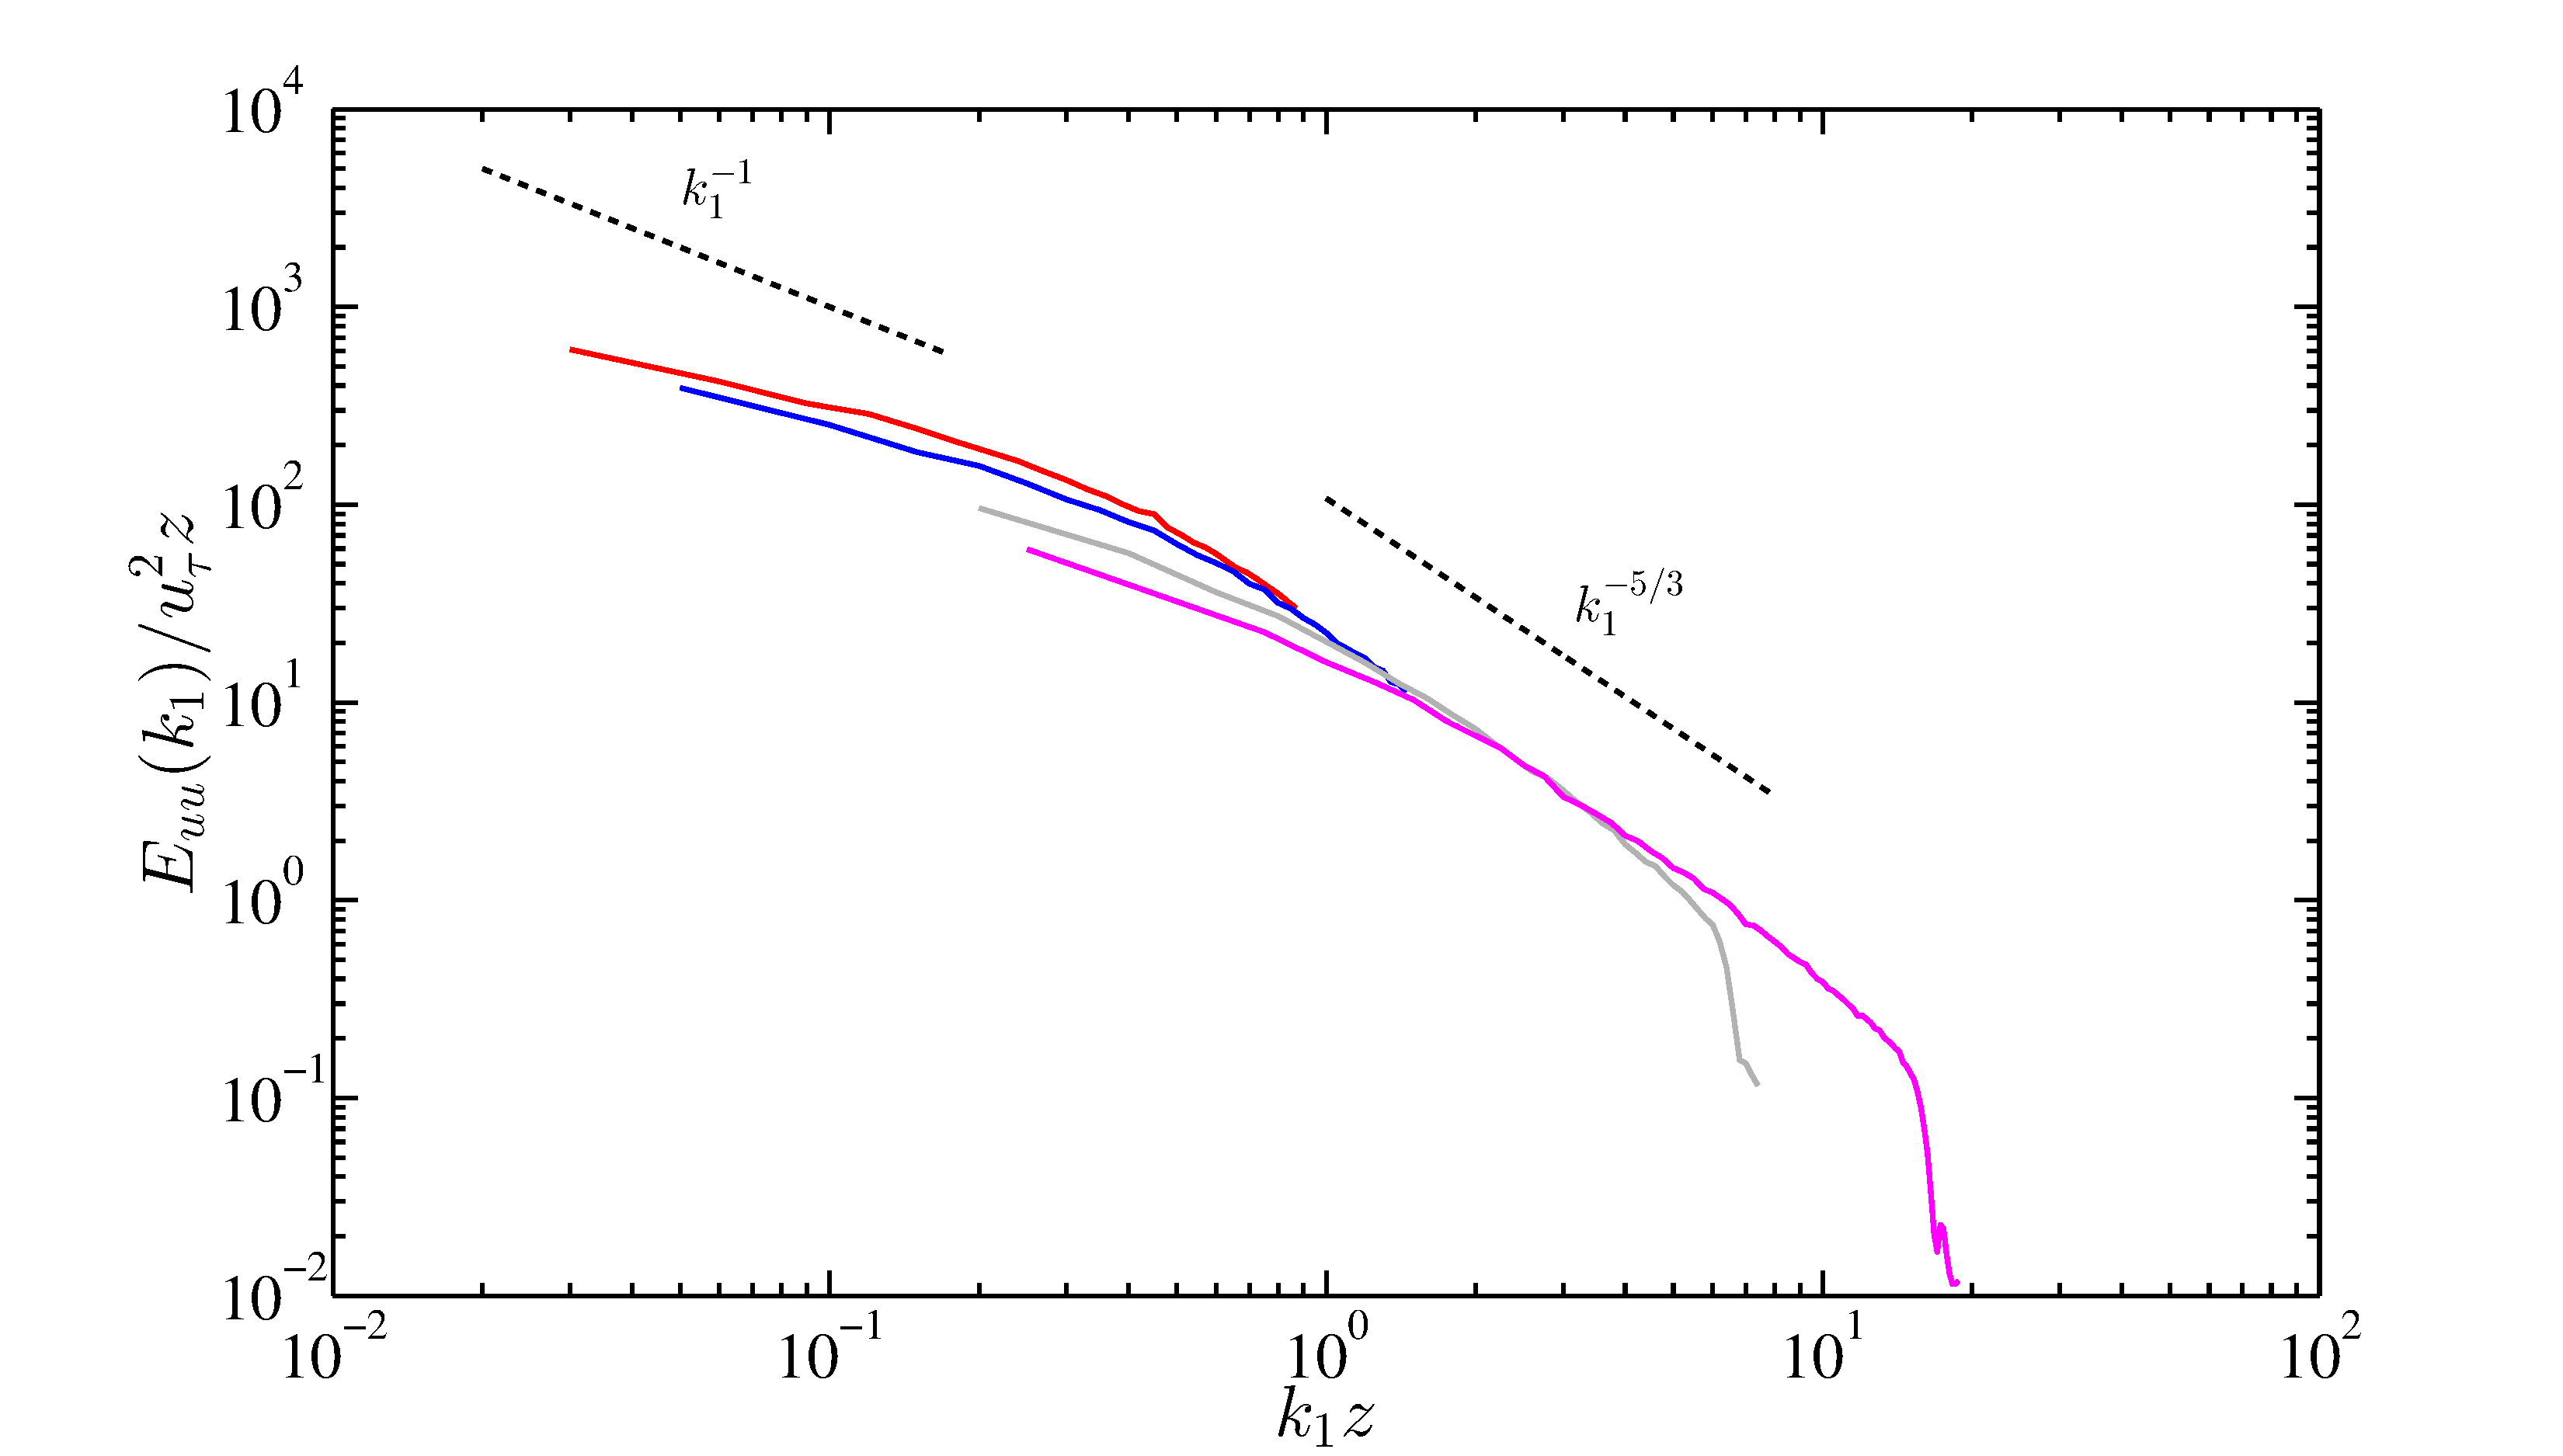
\includegraphics[width=\linewidth]{Fig2/energy_ABL_n05_filt4.pdf}
                \caption{}
                \label{fig:spec4}
        \end{subfigure}   
\centering
          \begin{subfigure}[t]{0.70\textwidth}
                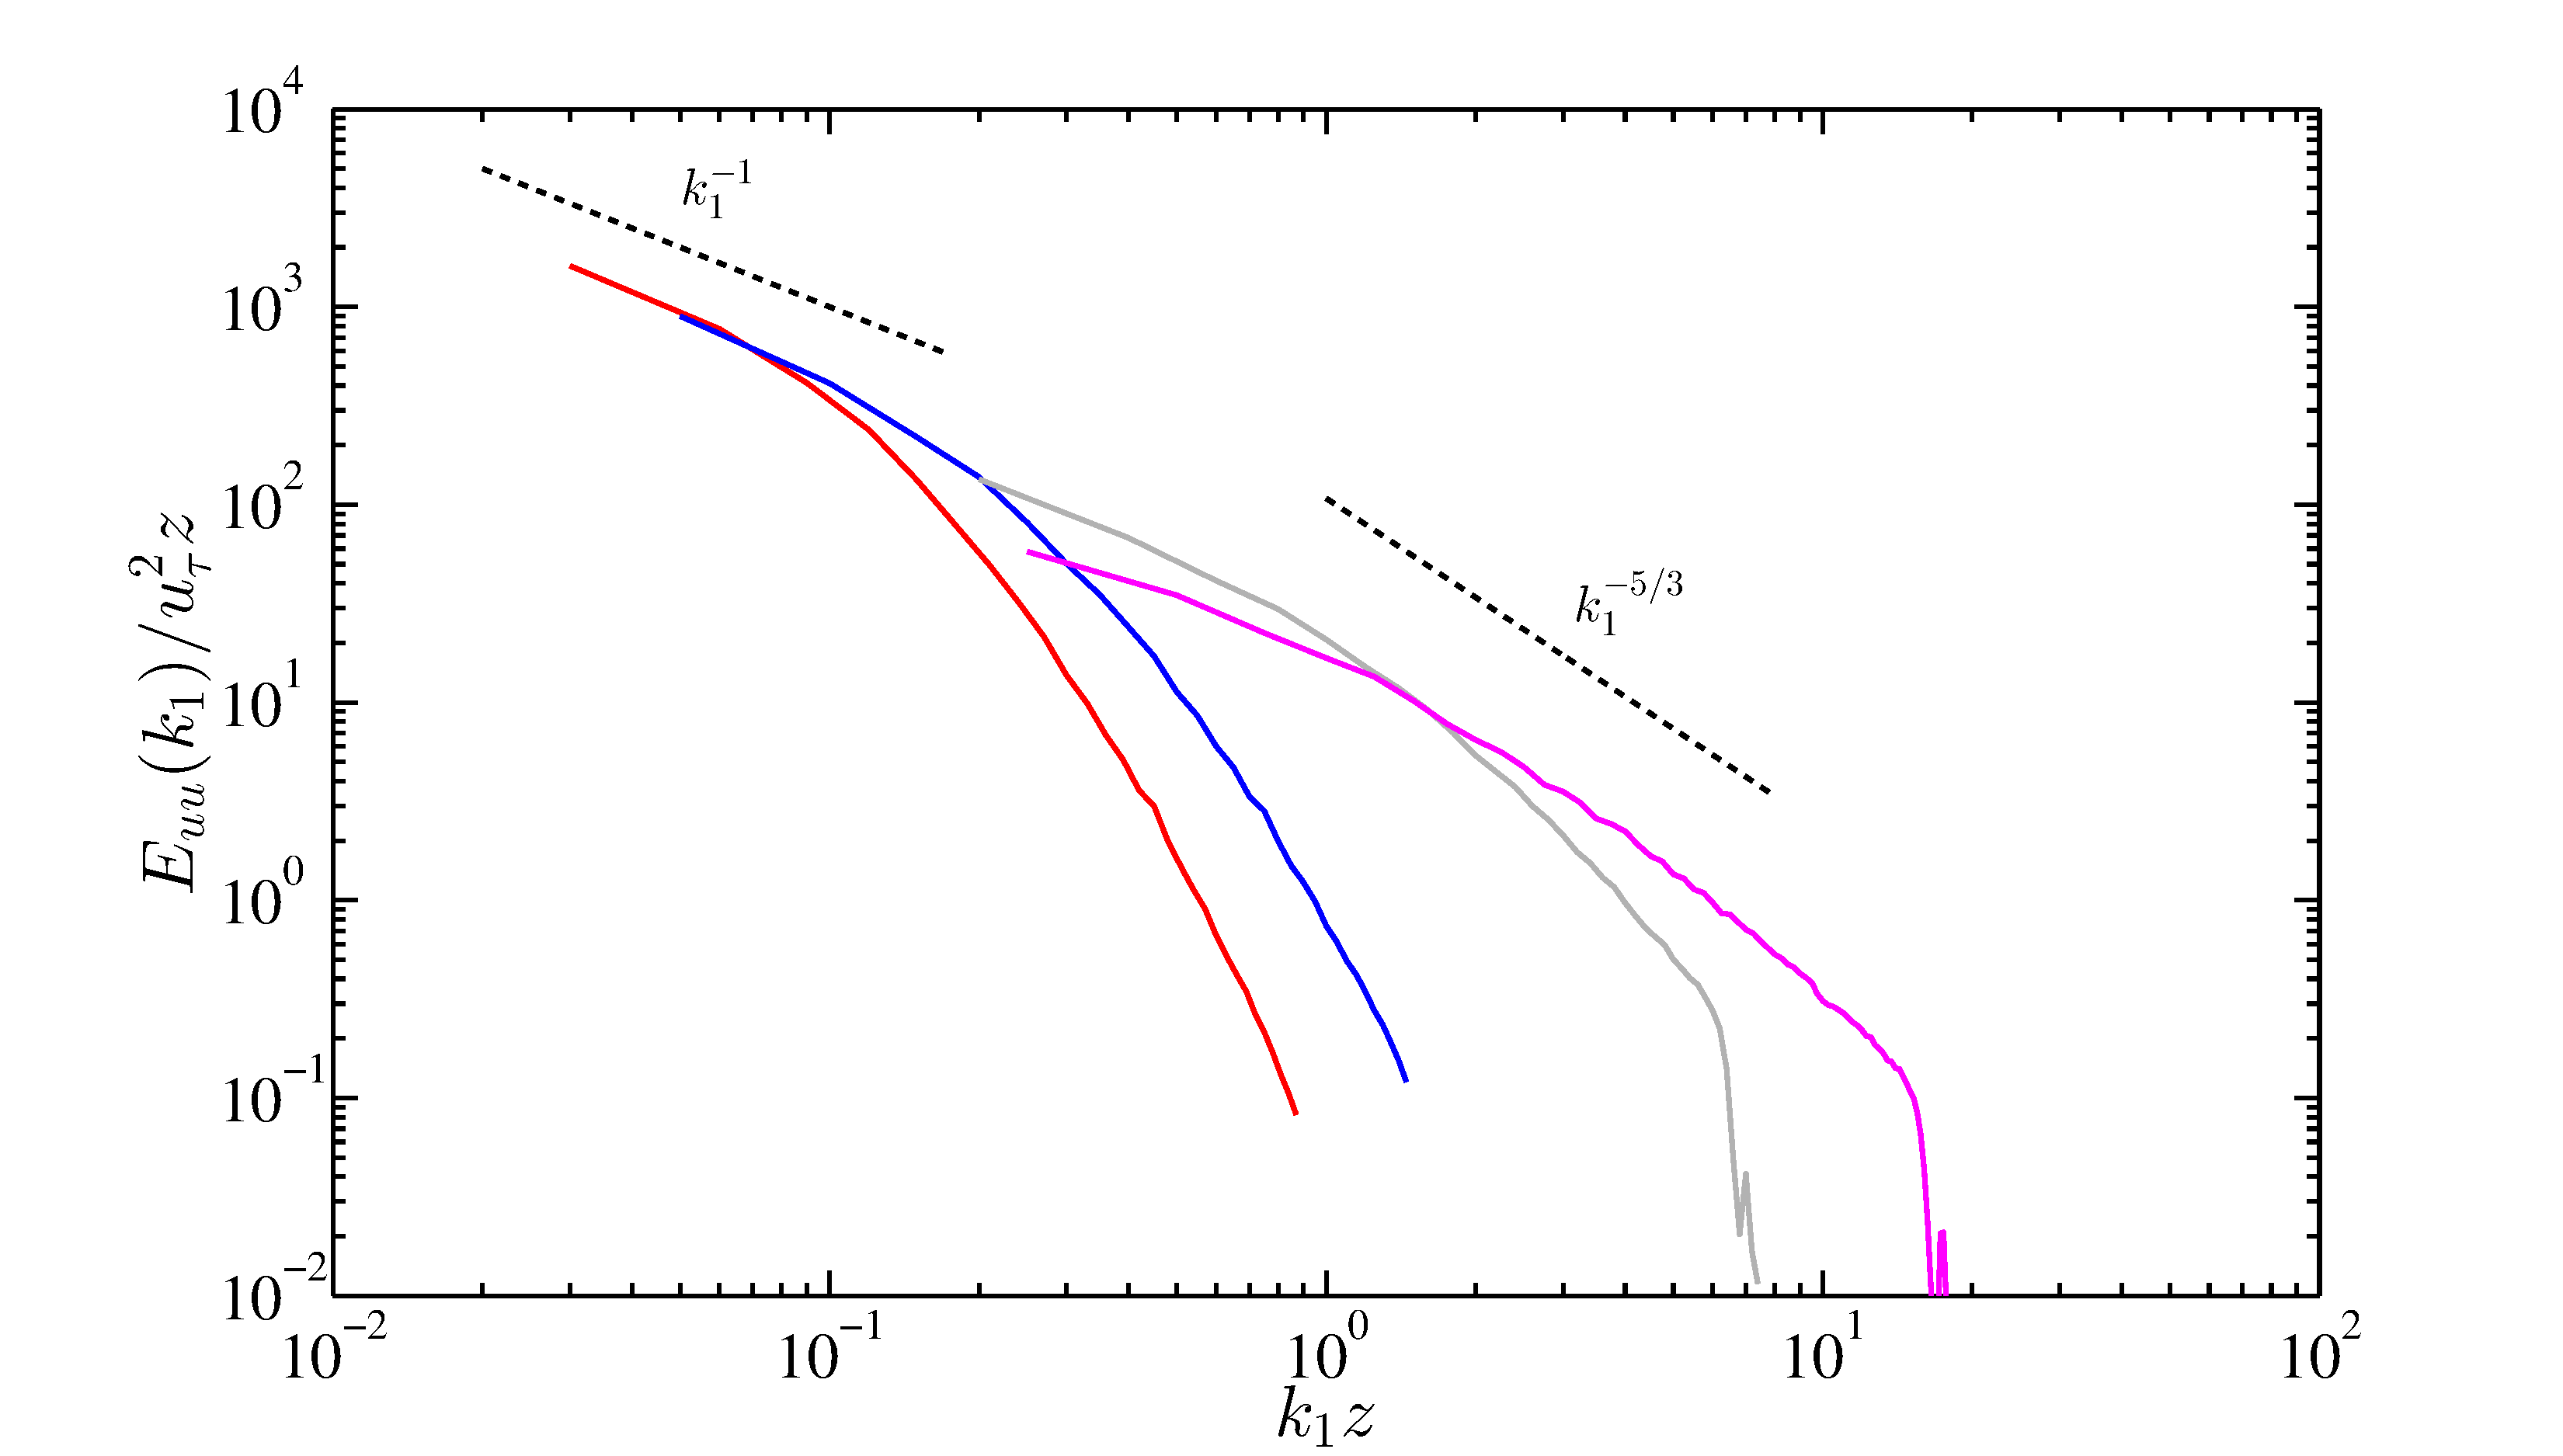
\includegraphics[width=\linewidth]{Fig2/energy_ABL_n2_filt4.pdf}
                \caption{}
                \label{fig:spec5}
        \end{subfigure}           
        \caption[1D Energy Spectra 2]{Temporally and Horizontally averaged streamwise energy spectrum (A) Case IX, $\lbrace C_0, \ n \rbrace = \lbrace 0.19 , 0.5 \rbrace$ (B) Case III, $\lbrace C_0, \ n \rbrace = \lbrace 0.16 , 2 \rbrace$, $k_c = 4$ is fixed. $k_1$ is the streamwise wavenumber. Red, $z/H = 0.015$, Blue, $z/H = 0.025$, Grey, $z/H = 0.1$, Magenta, $z/H = 0.25$  }\label{fig:stat0_lotw3}
\end{figure}

\begin{figure}
\centering
        \begin{subfigure}[t]{0.5\textwidth}
                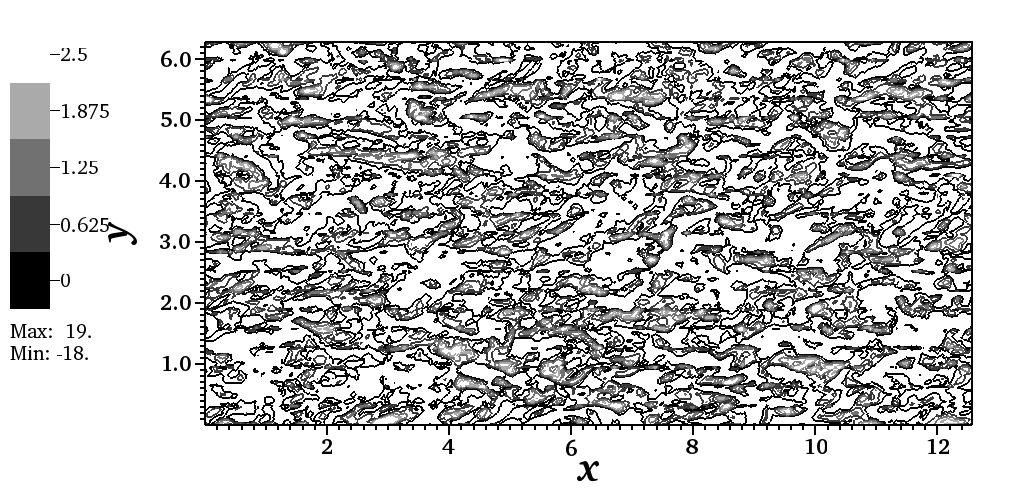
\includegraphics[width=\linewidth]{Fig2/x_vorticity_highdiff.png}
                \caption{}
                \label{fig:highdiff}
        \end{subfigure}%
        \centering
        \begin{subfigure}[t]{0.5\textwidth}
                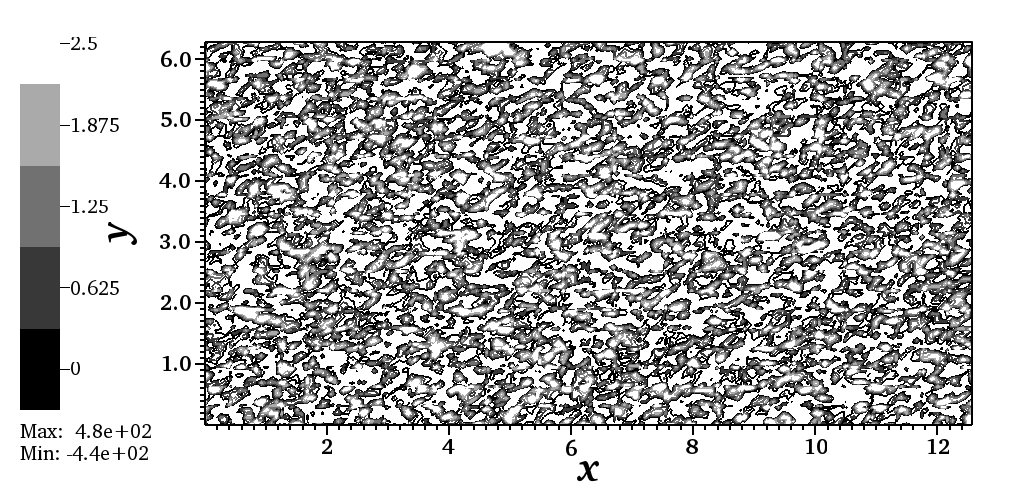
\includegraphics[width=\linewidth]{Fig2/x_vorticity_lowdiff.png}
                \caption{}
                \label{fig:lowdiff}
        \end{subfigure}
       \centering
        \begin{subfigure}[t]{0.5\textwidth}
                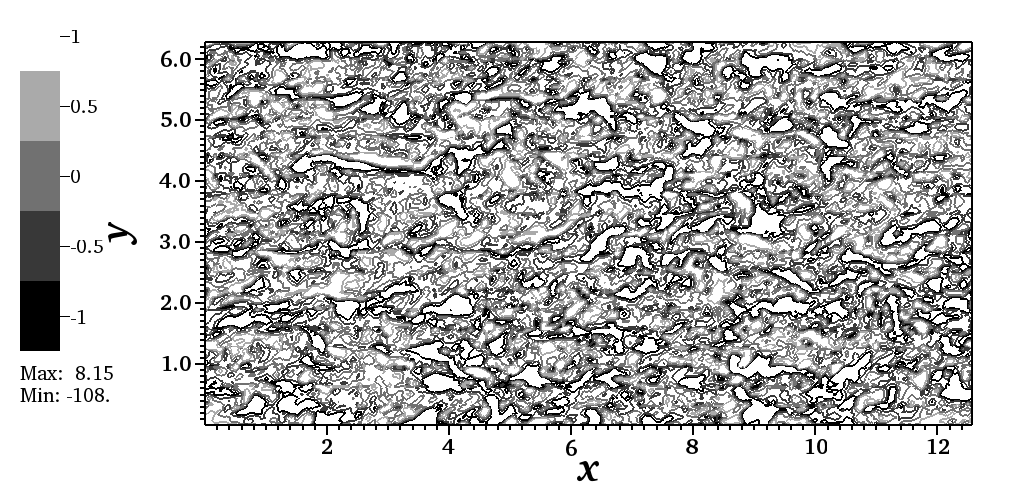
\includegraphics[width=\linewidth]{Fig2/z_vorticity_highdiff.png}
                \caption{}
                \label{fig:highdiff}
        \end{subfigure}%
        \centering
        \begin{subfigure}[t]{0.5\textwidth}
                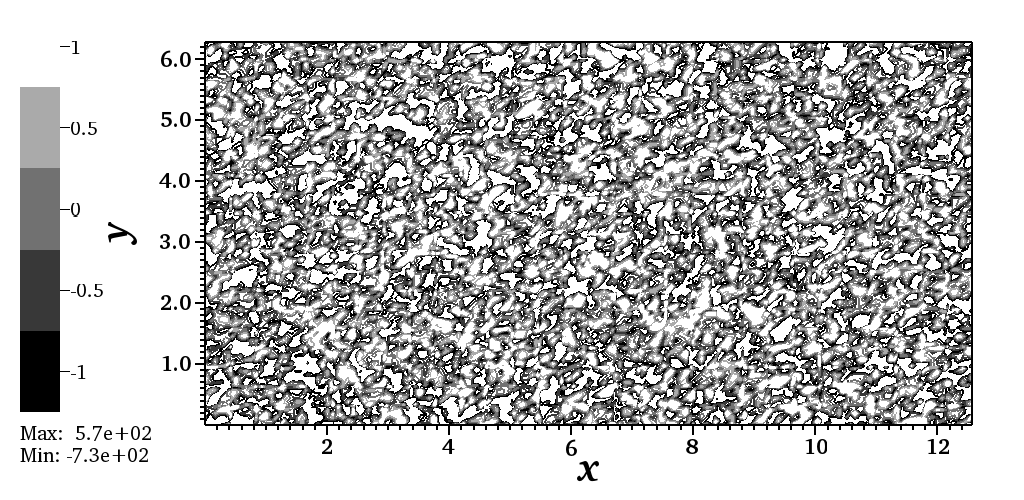
\includegraphics[width=\linewidth]{Fig2/z_vorticity_lowdiff.png}
                \caption{}
                \label{fig:lowdiff}
        \end{subfigure}%
        \caption[Near Wall vorticity structures]{ Instantaneous wall structures of $x$ (\textit{Top}), $z$ (\textit{Bottom}) vorticity  at log layer $z/H = 0.1$ (a) $\lbrace C_0 = 0.16,n = 2, k_c = 4\rbrace$ (b) $\lbrace C_0 = 0.19,n = 0.5, k_c = 4\rbrace $.}\label{fig:vort}
\end{figure}

\begin{figure}
\centering
        \begin{subfigure}[t]{0.5\textwidth}
                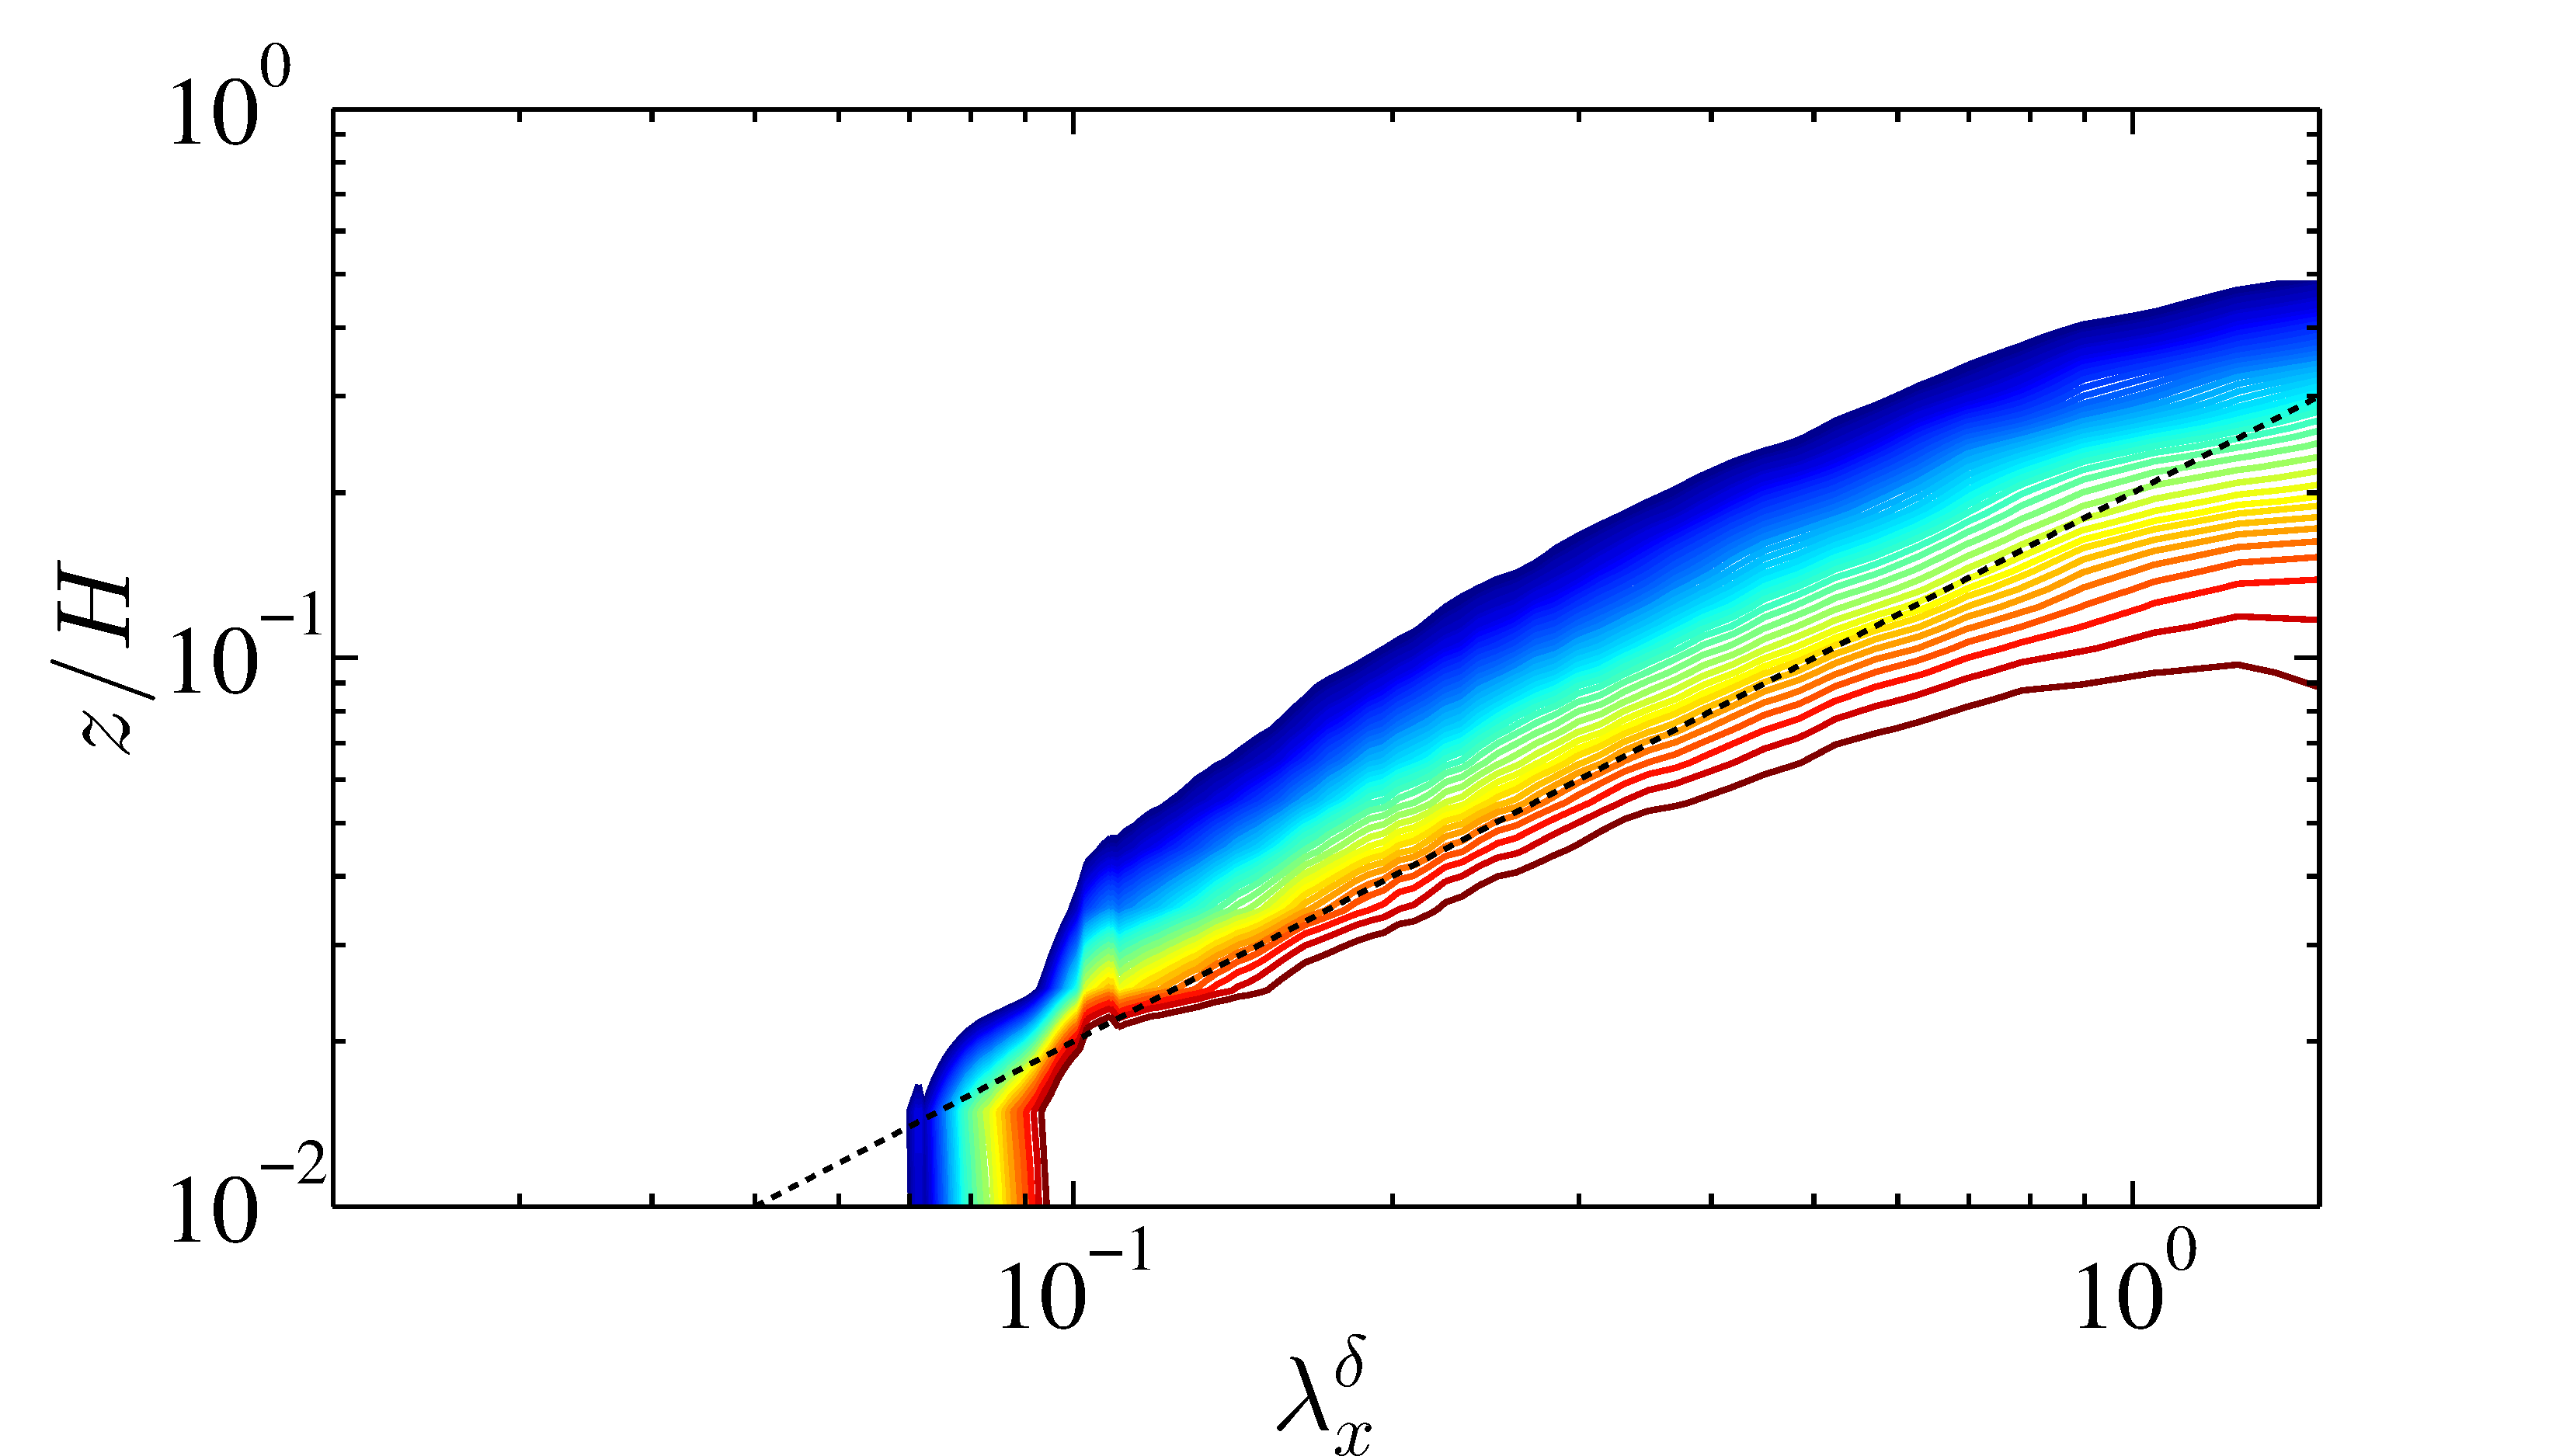
\includegraphics[width=\linewidth]{Fig2/energy_n05_logscale_85.pdf}
                \caption{}
                \label{fig:energy_n05}
        \end{subfigure}%
        \centering
        \begin{subfigure}[t]{0.5\textwidth}
                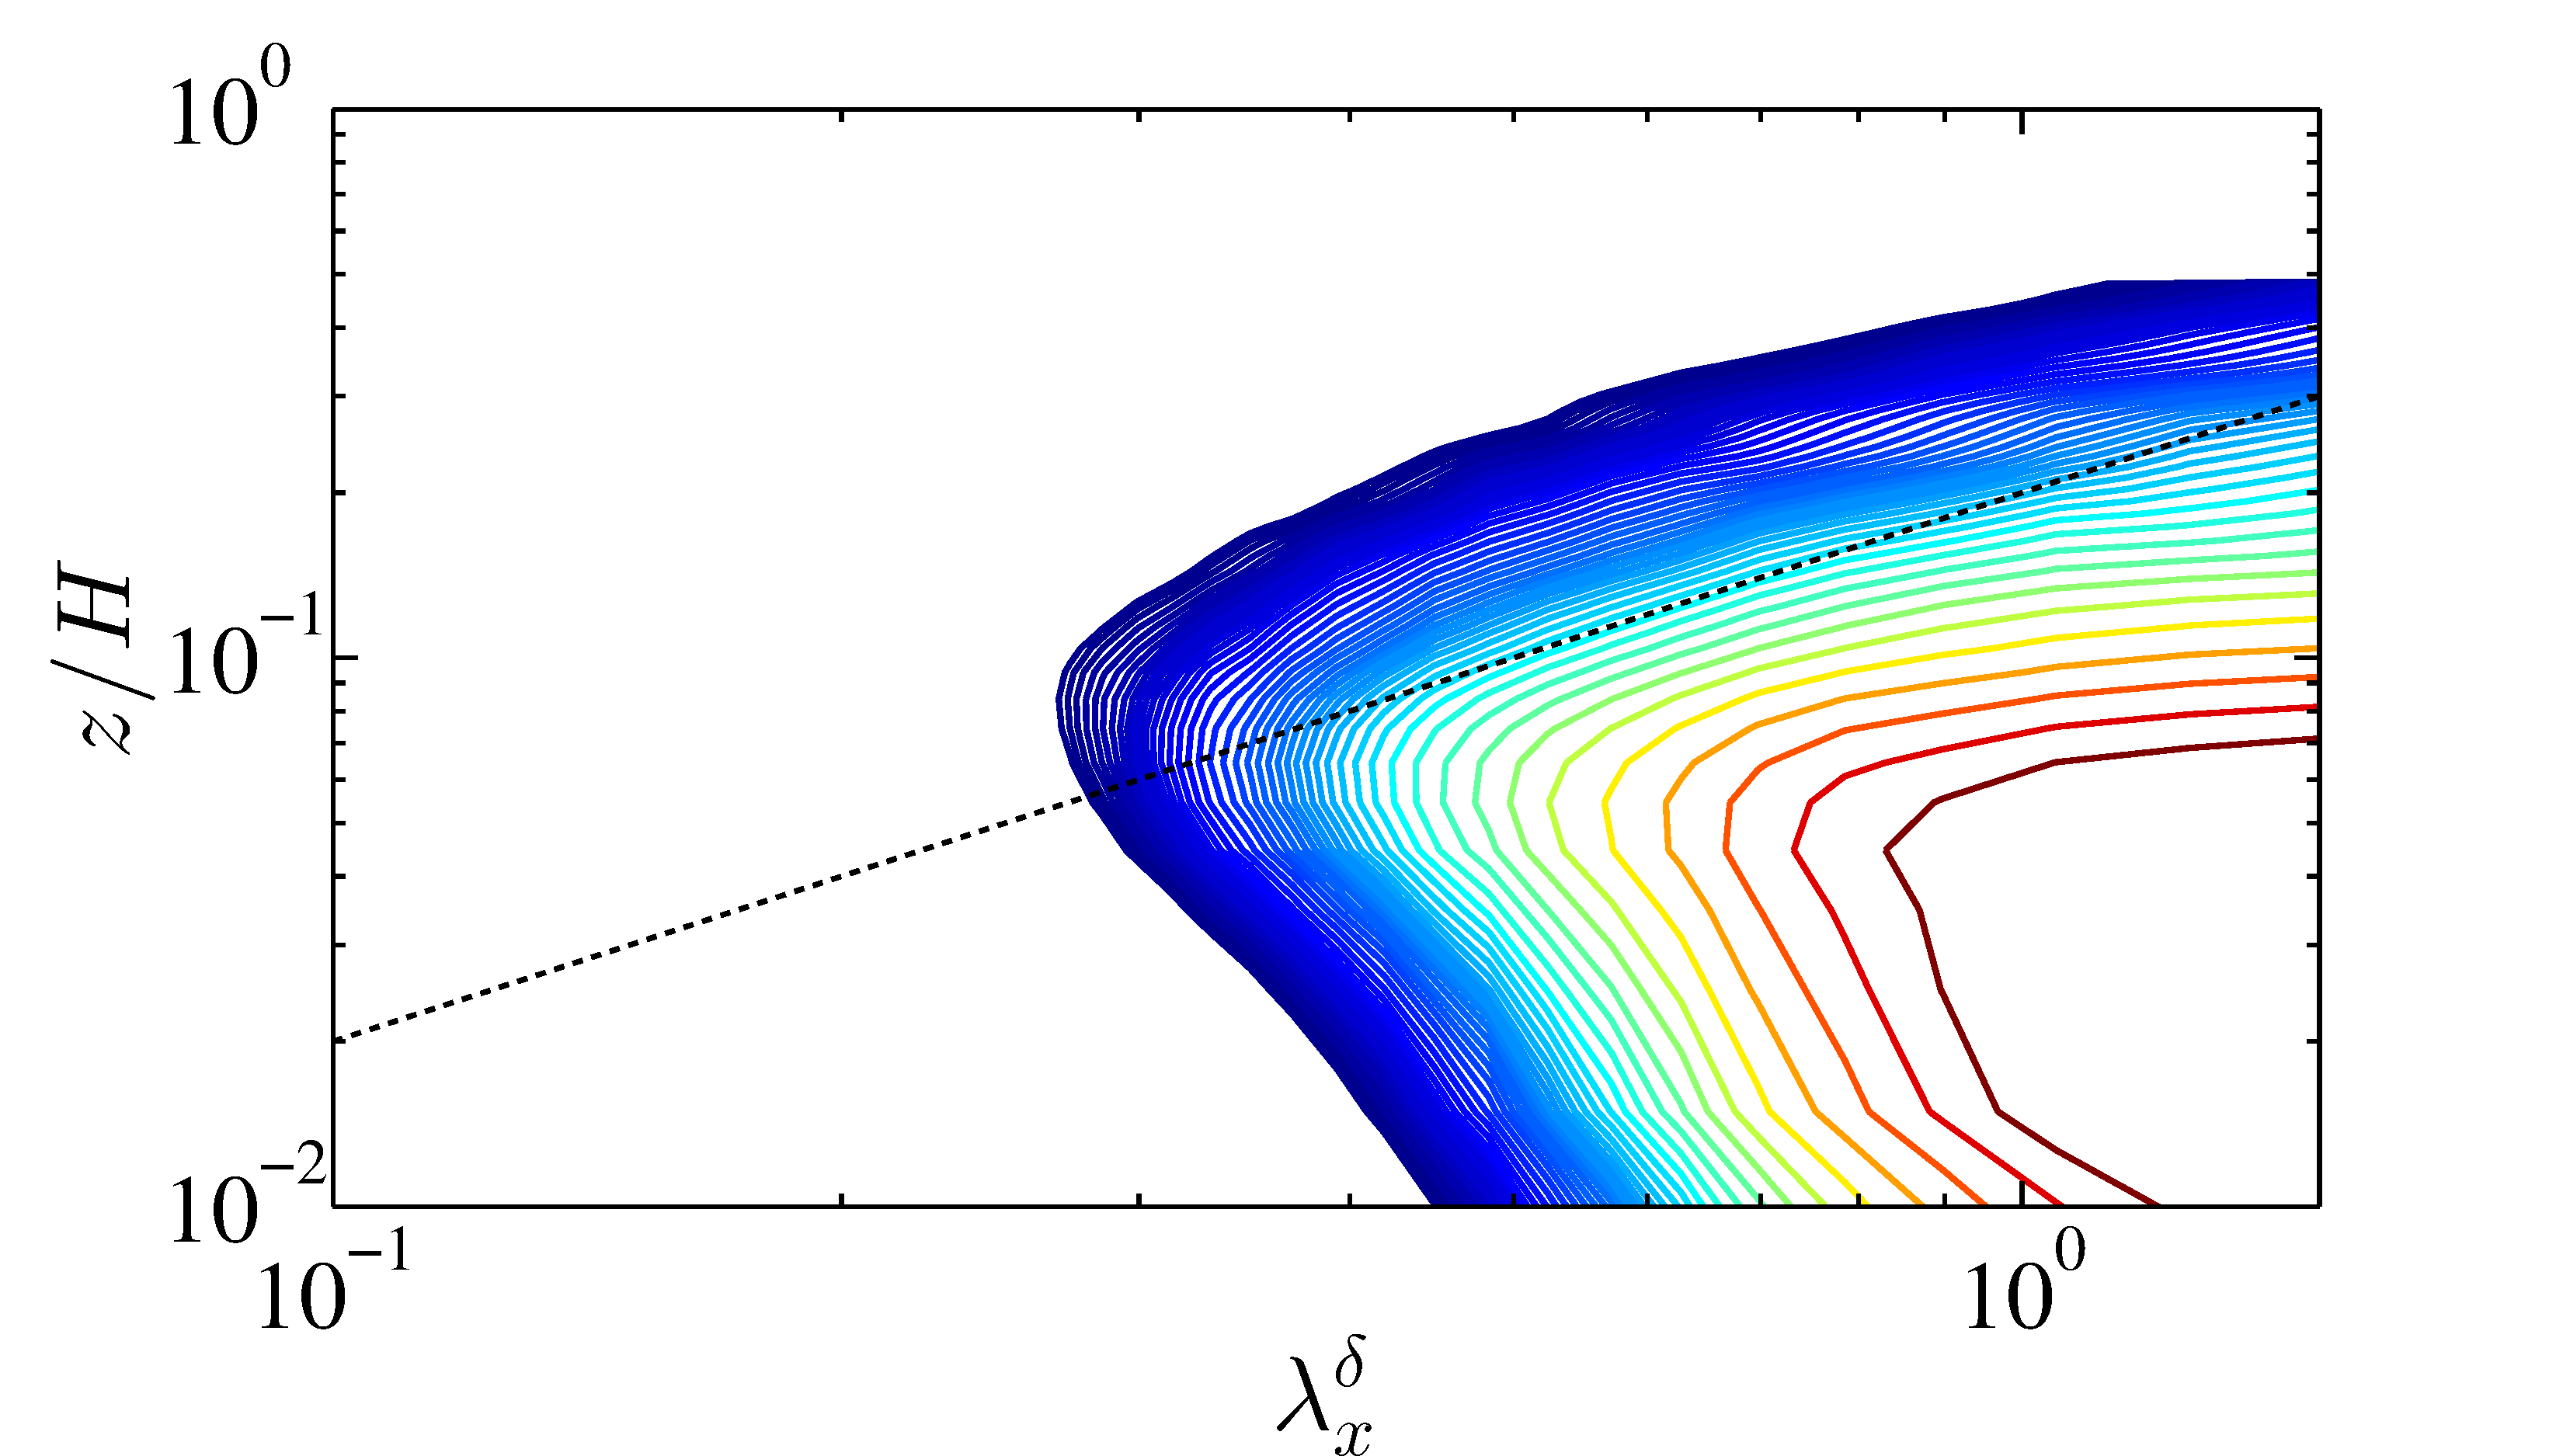
\includegraphics[width=\linewidth]{Fig2/energy_n2_logscale_85.pdf}
                \label{fig:energy_n2}
        \end{subfigure}%
        \caption[Log variation of Energy]{Variation of horizontally and temporally averaged Premultiplied energy spectra $k_1E_{uu}(k_1)$ over wall-normal distance $z/H$ and normalized length scale $\lambda^{\delta}_{x}$ (A) Case IX, $\lbrace C_0 = 0.19,n = 0.5, k_c = 4\rbrace $ (B) Case III, $\lbrace C_0 = 0.16,n = 2, k_c = 4\rbrace $. $\lambda^{\delta}_{x} = \frac{\lambda_x}{H}$, is the normalized streamwise wavelength. $\lambda_x = \frac{2\pi}{k_1}$. Dashed line represents $\lambda_x^{\delta} = 5z/H$. Contour levels indicate $0.85$ times the maximum value at each $z$ level.}\label{fig:2d_spec}
\end{figure}

\begin{figure}
\centering
        \begin{subfigure}[t]{0.5\textwidth}
                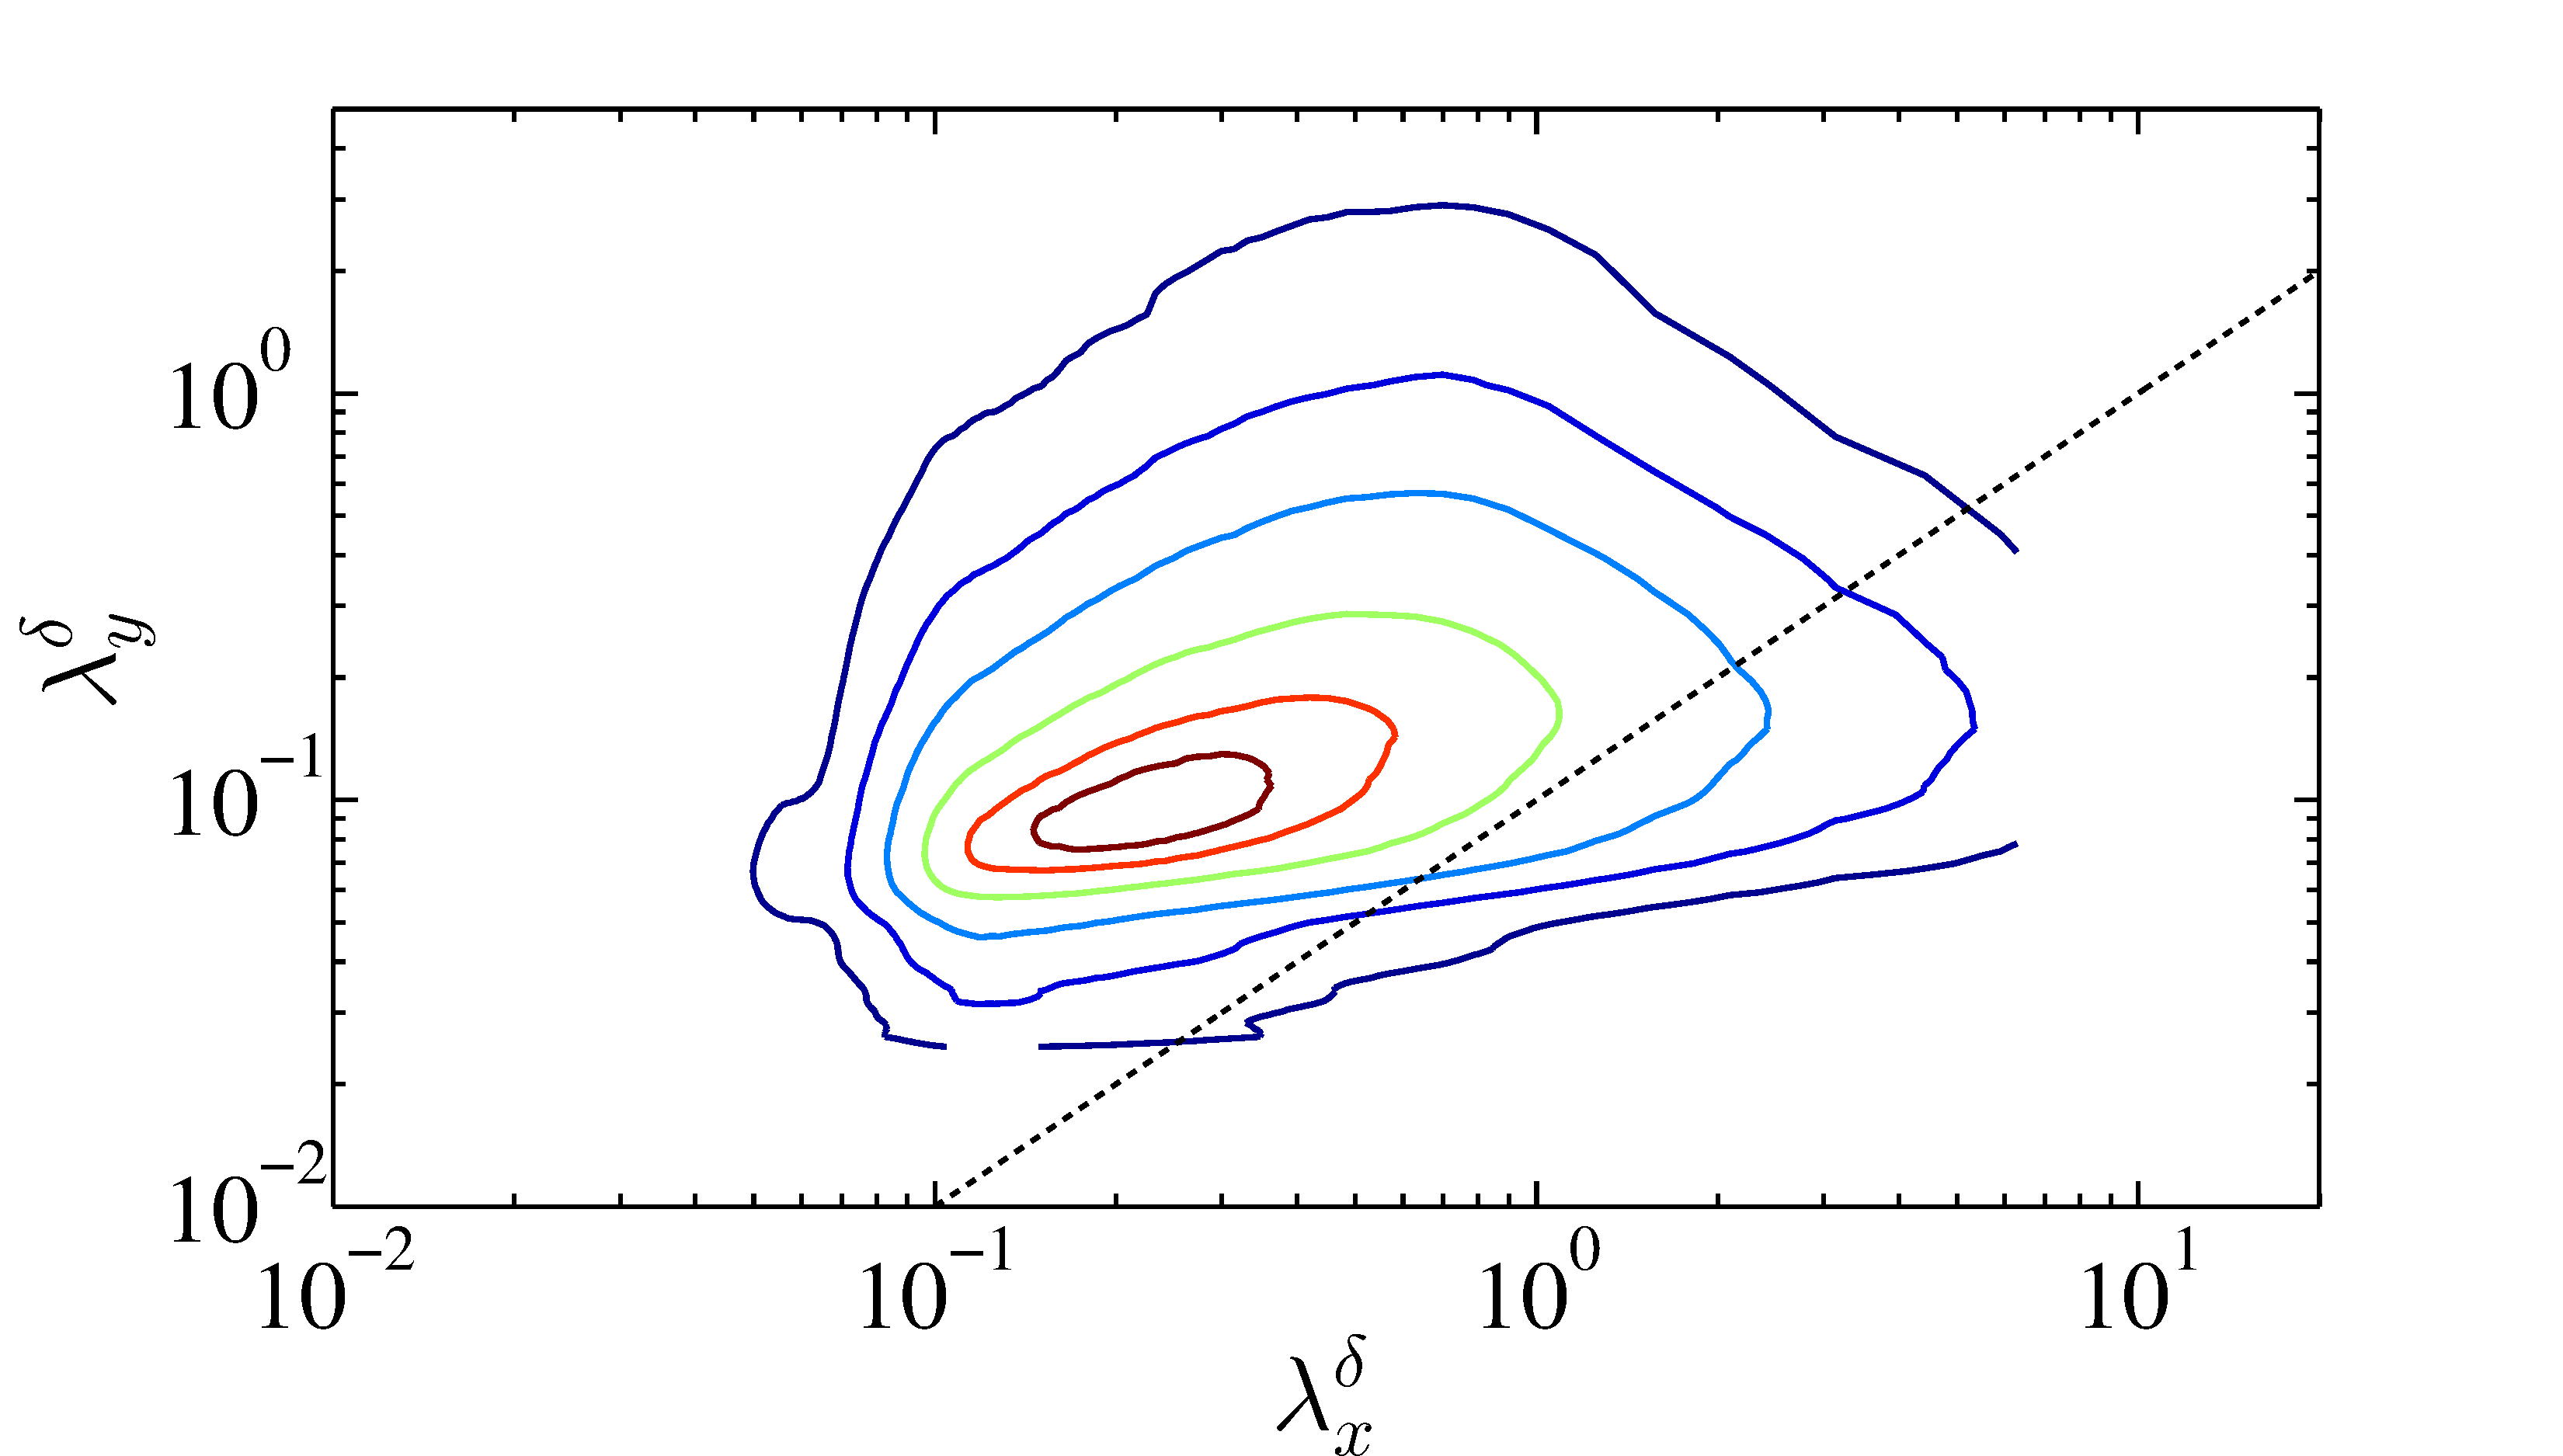
\includegraphics[width=\linewidth]{Fig2/energy_contour_ABL_n05_filt2_level2.pdf}
                \caption{}
                \label{fig:energy1}
        \end{subfigure}%
        \centering
        \begin{subfigure}[t]{0.5\textwidth}
                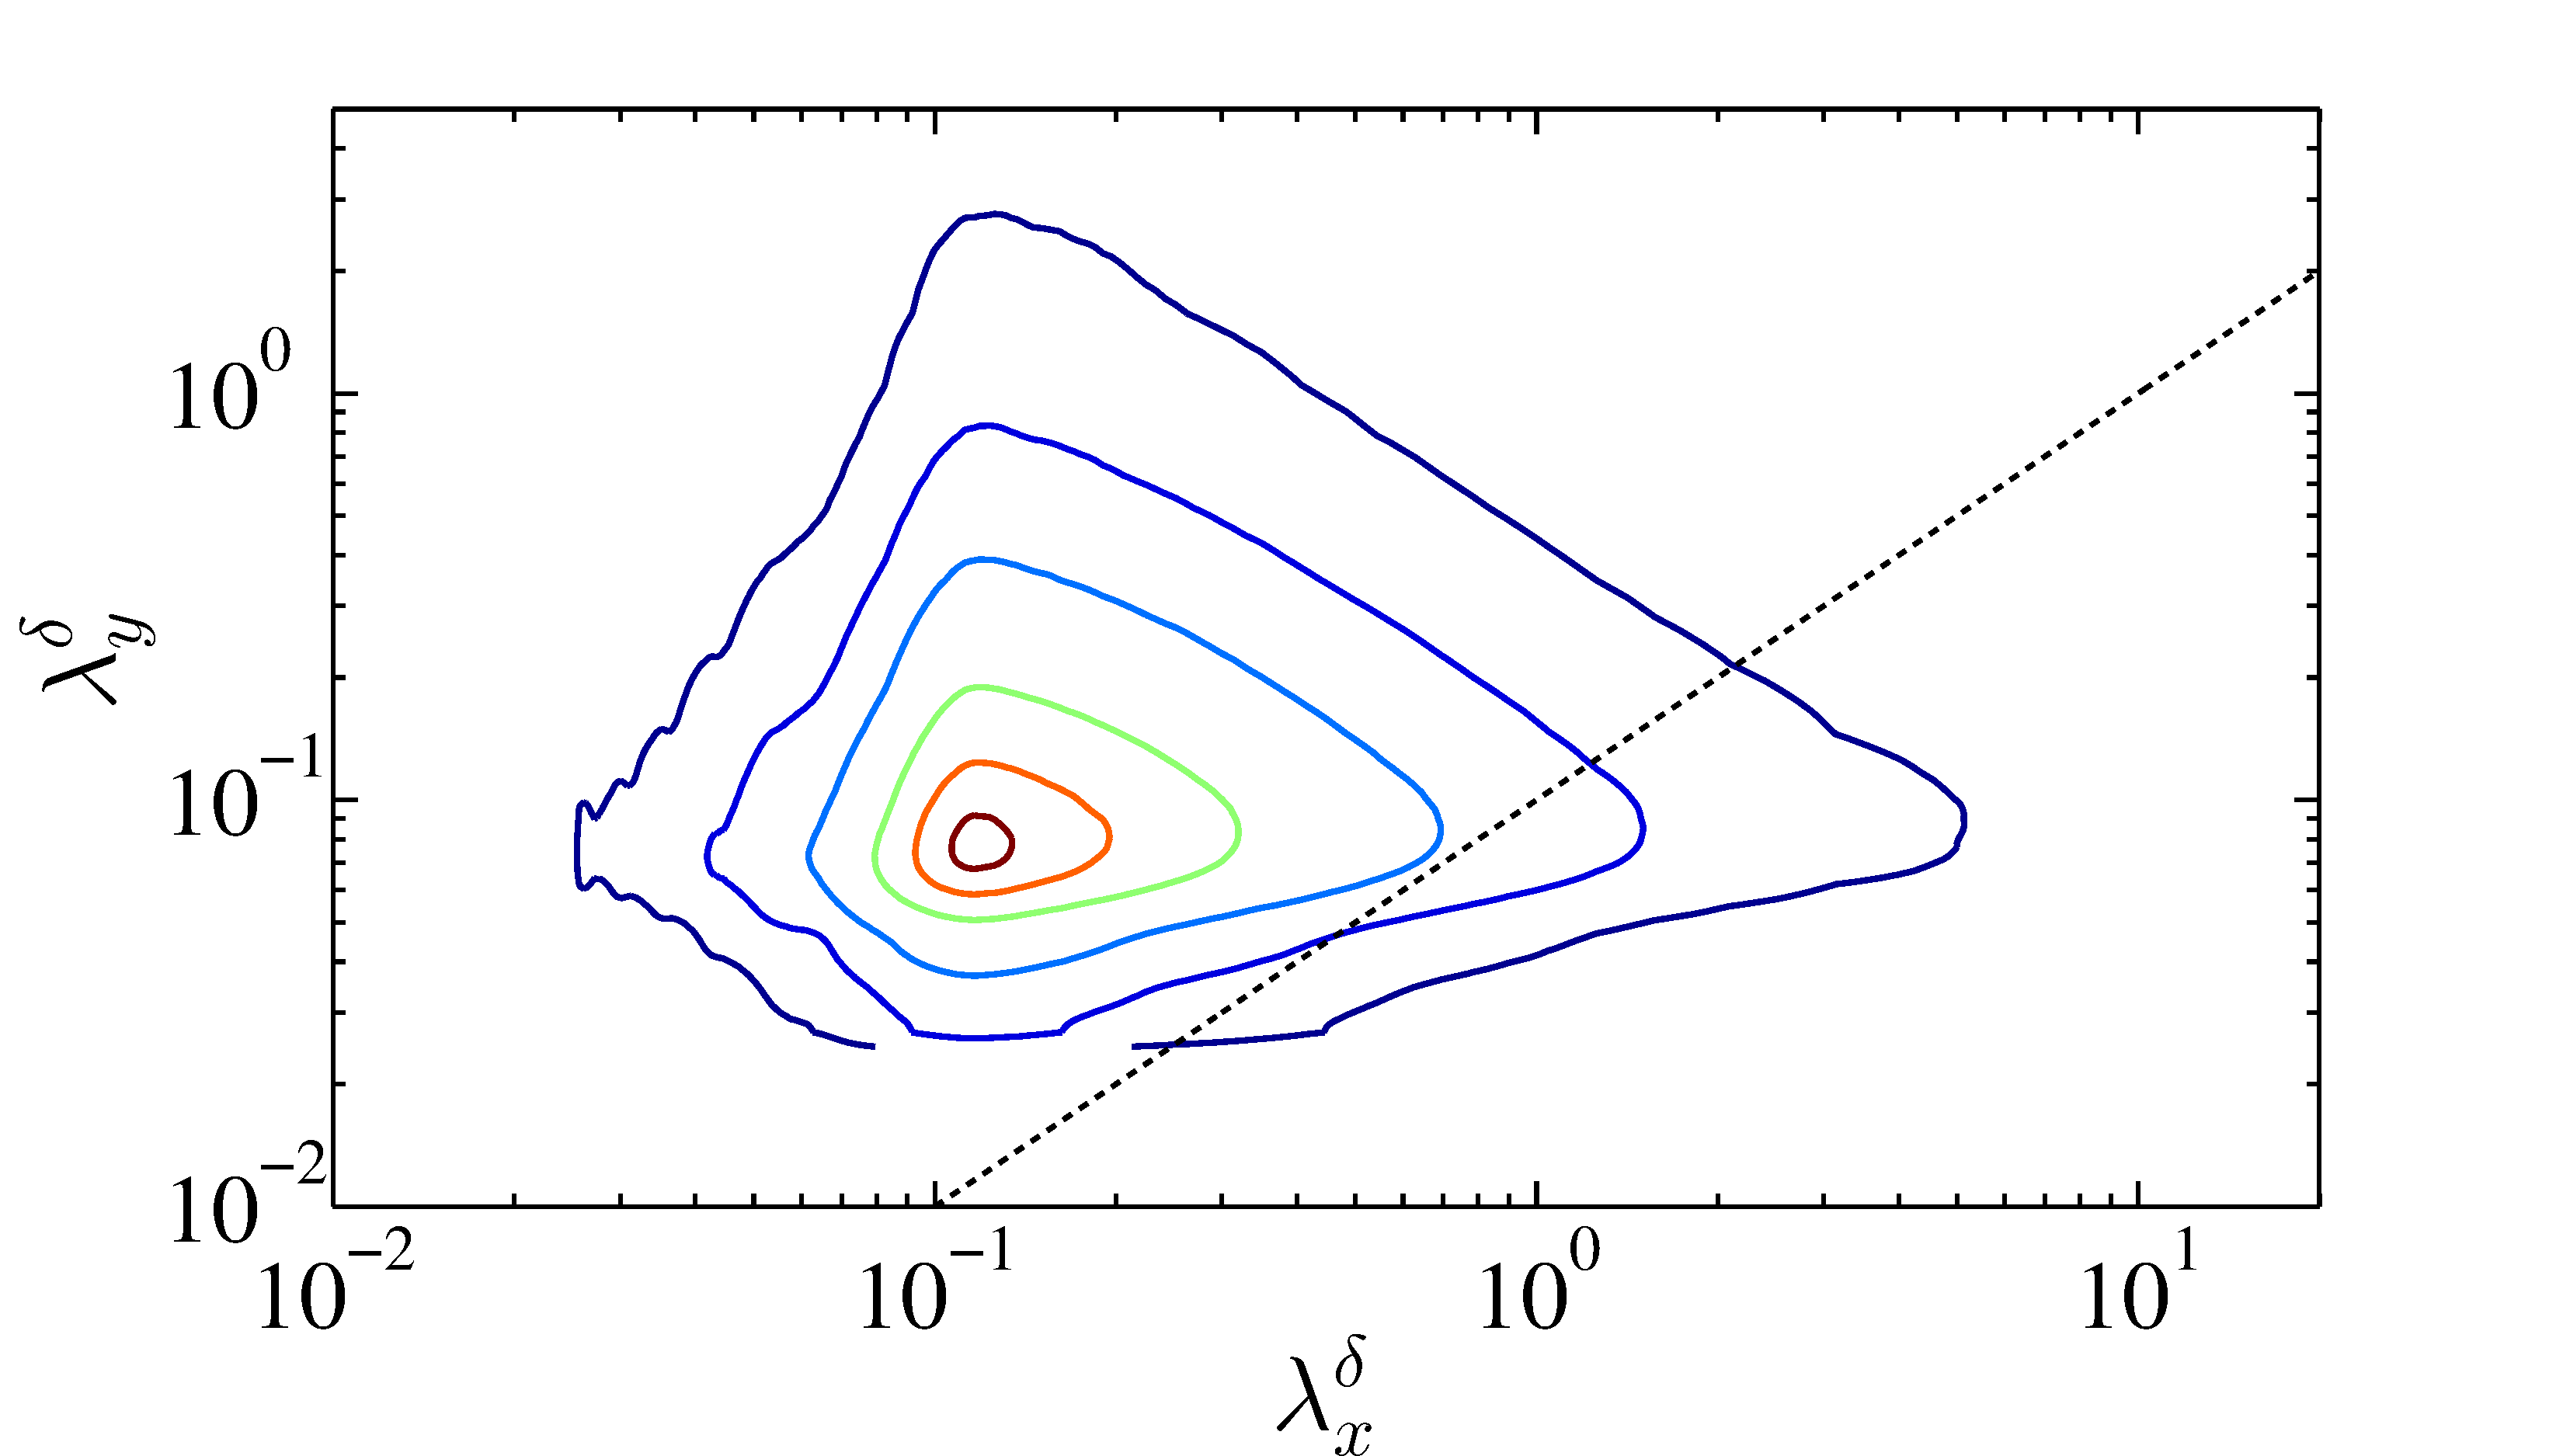
\includegraphics[width=\linewidth]{Fig2/dissp_contour_ABL_n05_filt2_level2.pdf}
                \caption{}
                \label{fig:dissip1}
        \end{subfigure}
\centering
        \begin{subfigure}[t]{0.5\textwidth}
                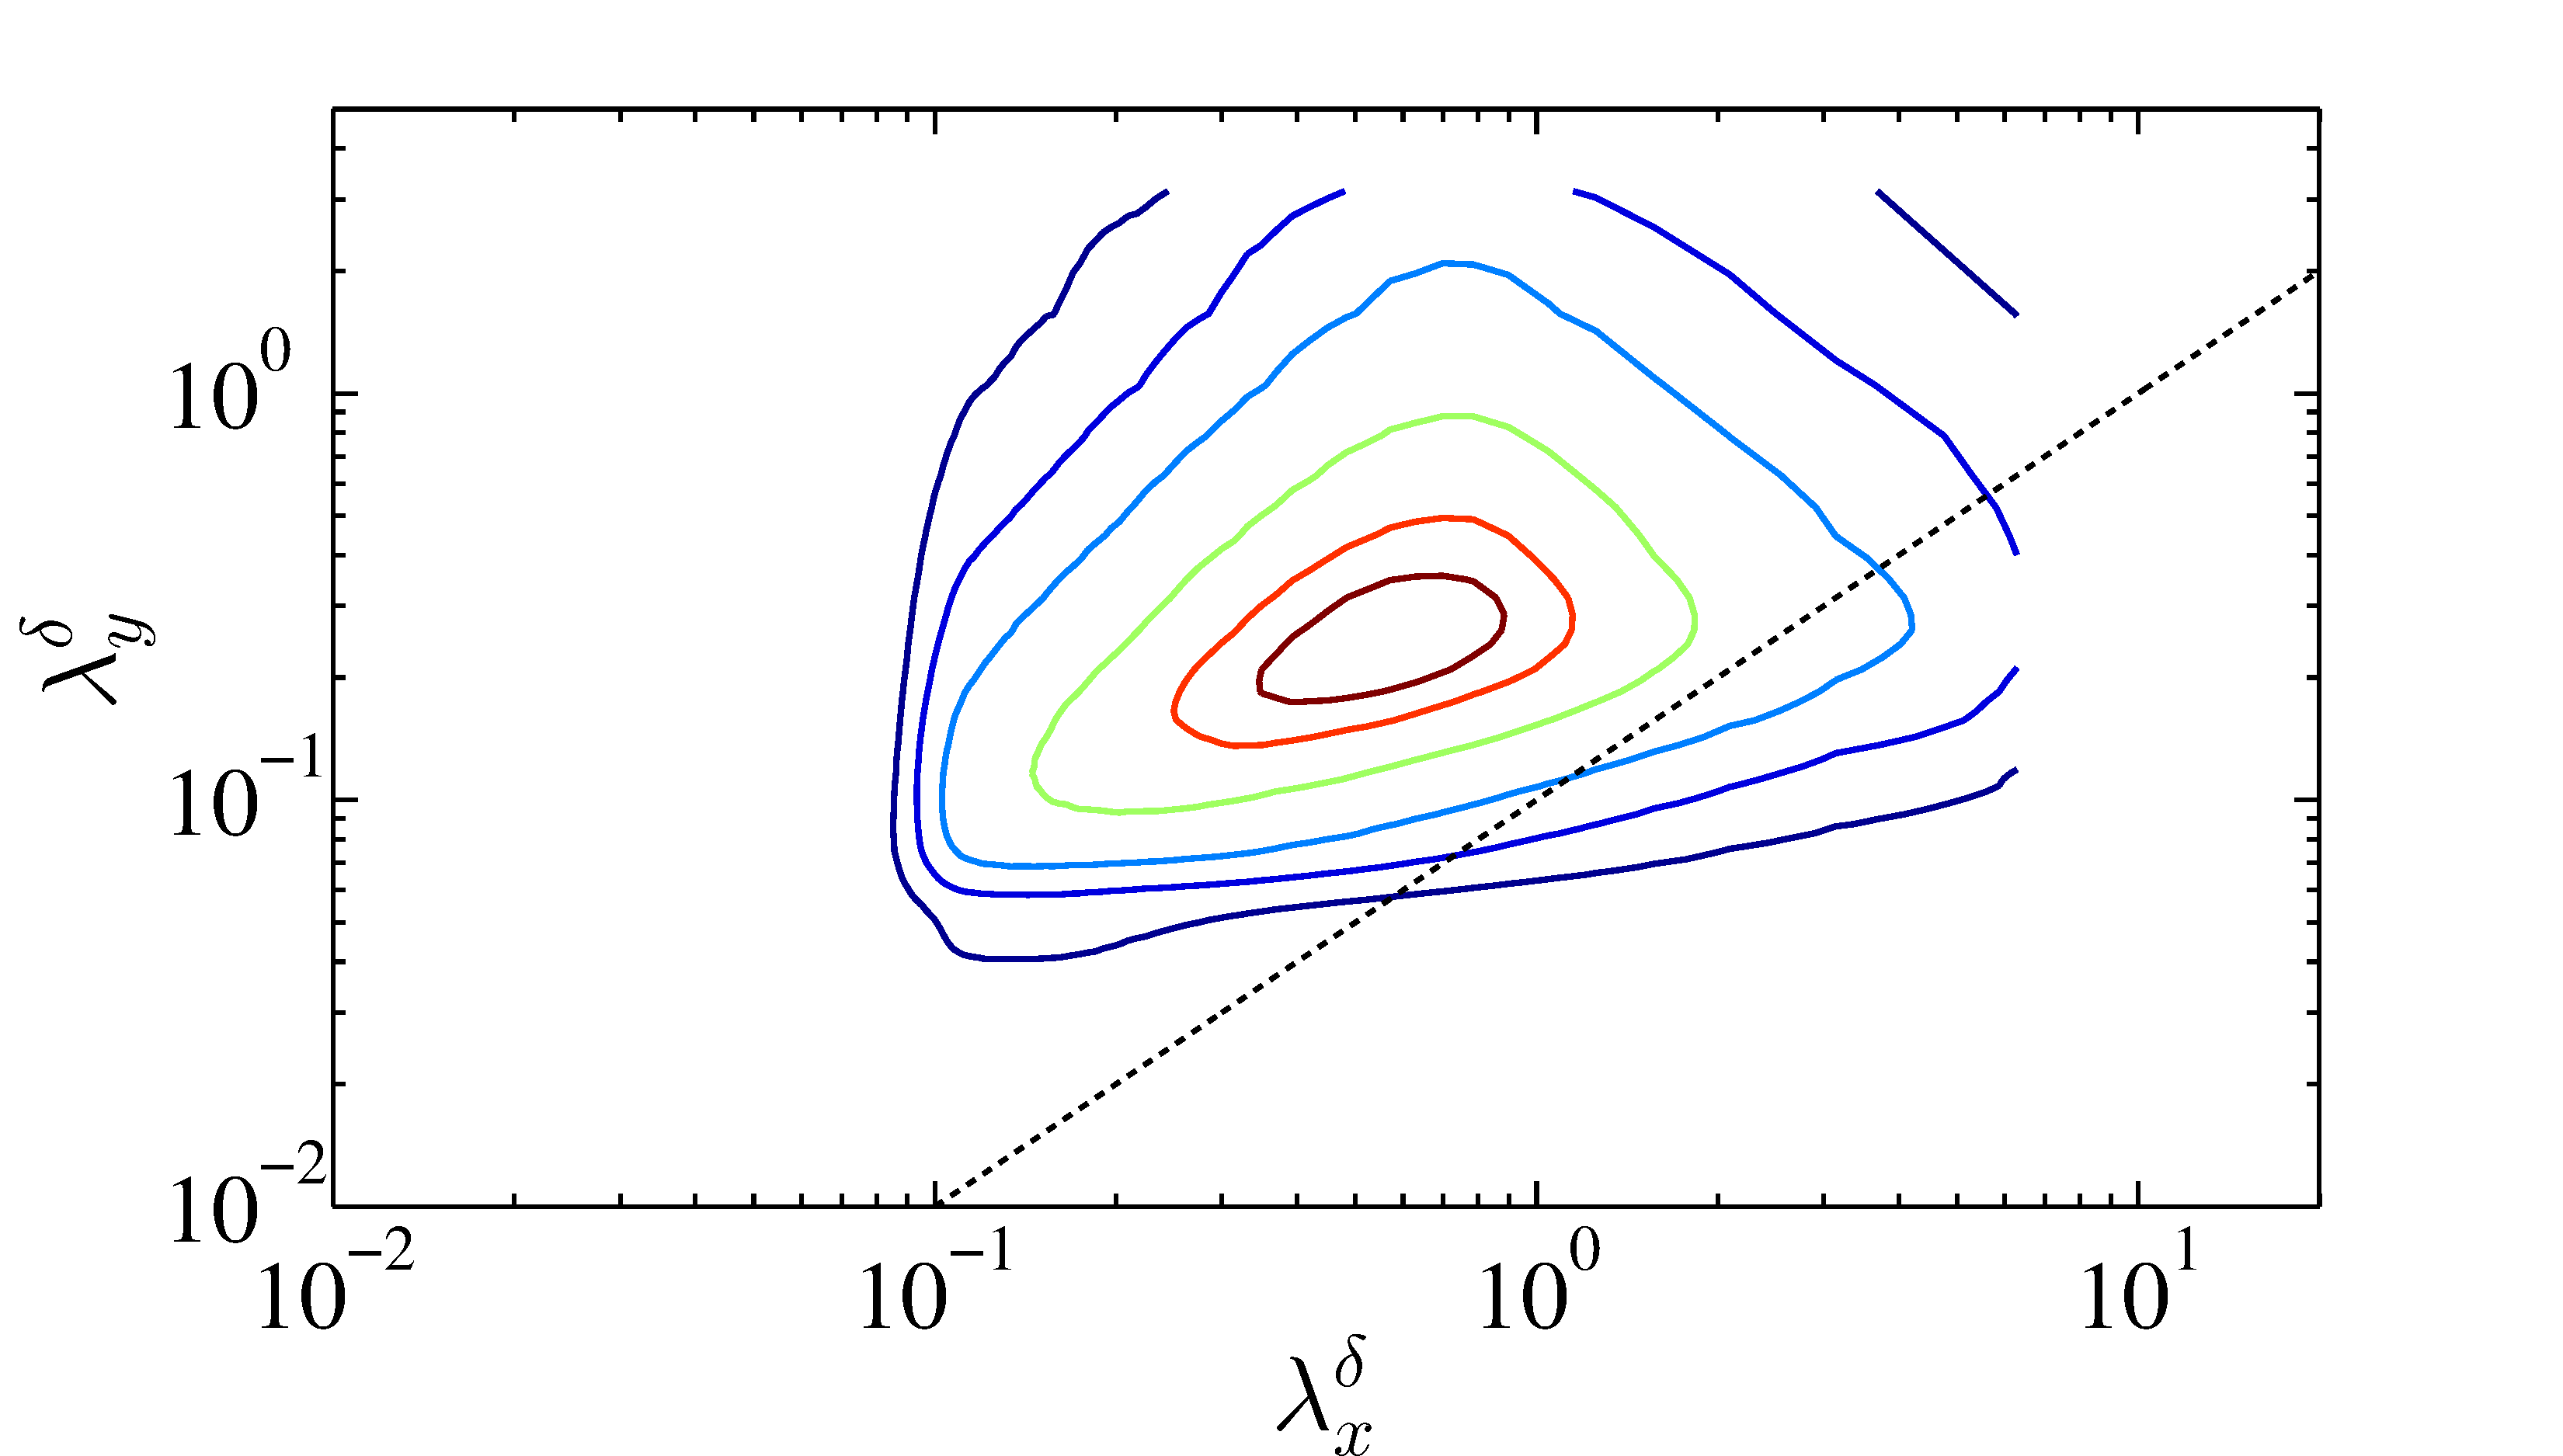
\includegraphics[width=\linewidth]{Fig2/energy_contour_ABL_n05_filt2_level4.pdf}
                \caption{}
                \label{fig:energy2}
        \end{subfigure}%
        \centering
        \begin{subfigure}[t]{0.5\textwidth}
                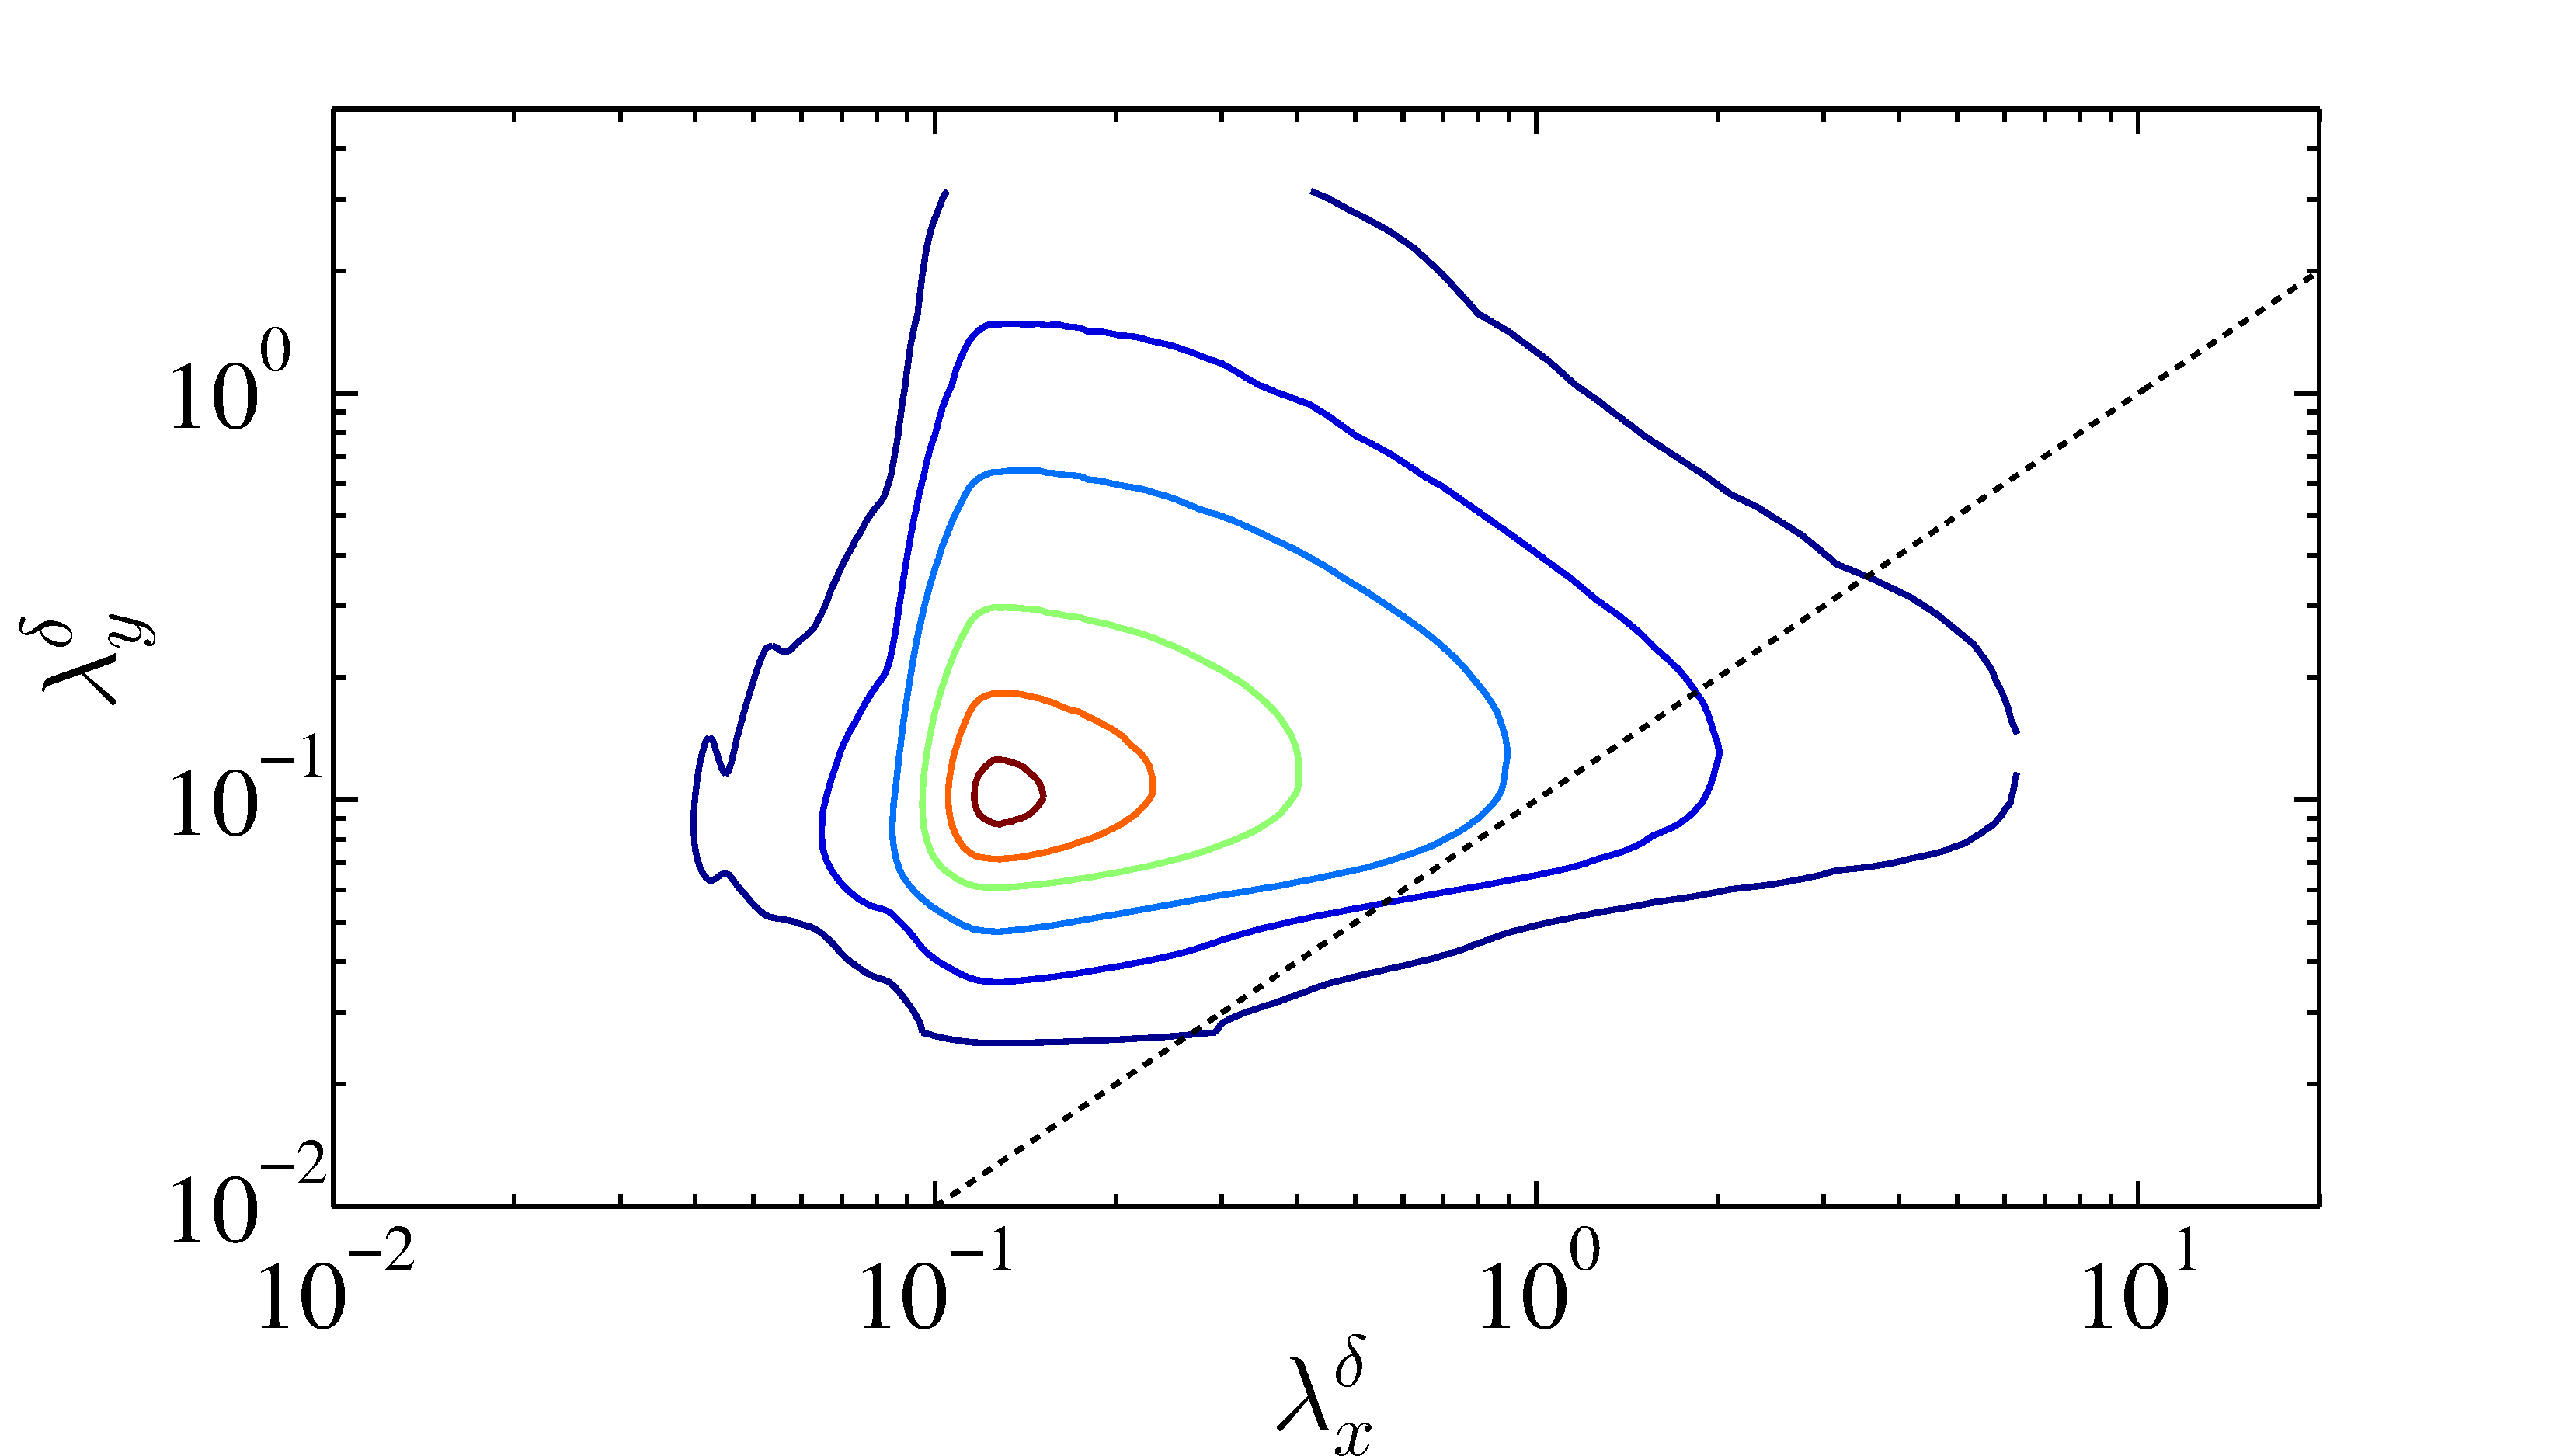
\includegraphics[width=\linewidth]{Fig2/dissp_contour_ABL_n05_filt2_level4.pdf}
                \caption{}
                \label{fig:dissip2}
        \end{subfigure}
 \centering
        \begin{subfigure}[t]{0.5\textwidth}
                \includegraphics[width=\linewidth]{Fig2/energy_contour_ABL_n05_filt2_level5.pdf}
                \caption{}
                \label{fig:energy3}
        \end{subfigure}%
        \centering
        \begin{subfigure}[t]{0.5\textwidth}
                \includegraphics[width=\linewidth]{Fig2/dissp_contour_ABL_n05_filt2_level5.pdf}
                \caption{}
                \label{fig:dissip3}
        \end{subfigure}              
        
        \caption[Premultiplied Spectra 1]{2D Premultiplied spectra for Case IX ($\lbrace C_0 = 0.19, n = 0.5, k_c = 4\rbrace$) in the plane of normalized wavelengths $\lambda_x^{\delta}$ and $\lambda_y^{\delta}$, normalized by BL thickness $H$. Left: Streamwise energy spectra $k_xk_zE_{uu}(k_x,k_z)$, Right: Enstrophy spectra $k_xk_zE_{\omega\omega}(k_x,k_z)$, $(k_x, k_z)$: streamwise and spanwise wavenumbers respectively. (A)-(B) $z/H = 0.015$; (C)-(D) $z/H = 0.1$; (E)-(F) $z/H = 0.25$. Six contour levels are [0.05 0.125 0.25 0.5 0.75 0.95] times the maximum, with increasing from red to blue. Smallest enclosed contour is the maximum The dashed line represents $\lambda_x^{\delta} = 10 \lambda_y^{\delta}$}\label{fig:2d_spec_diss}
\end{figure}

\begin{figure}
\centering
        \begin{subfigure}[t]{0.5\textwidth}
                \includegraphics[width=\linewidth]{Fig3/energy_contour_ABL_n2n05_level2.pdf}
                \caption{}
                \label{fig:energy1b}
        \end{subfigure}%
        \centering
        \begin{subfigure}[t]{0.5\textwidth}
                \includegraphics[width=\linewidth]{Fig3/energy_contour_ABL_n2n05_level5.pdf}
                \caption{}
                \label{fig:dissip1b}
        \end{subfigure}
\centering
        \begin{subfigure}[t]{0.5\textwidth}
                \includegraphics[width=\linewidth]{Fig3/dissp_contour_ABL_n2n05_level2.pdf}
                \caption{}
                \label{fig:energy2b}
        \end{subfigure}%
        \centering
        \begin{subfigure}[t]{0.5\textwidth}
                \includegraphics[width=\linewidth]{Fig3/dissp_contour_ABL_n2n05_level5.pdf}
                \caption{}
                \label{fig:dissip2b}
        \end{subfigure}
 \centering
        \begin{subfigure}[t]{0.5\textwidth}
                \includegraphics[width=\linewidth]{Fig3/cospectra_contour_ABL_n2n05_level2.pdf}
                \caption{}
                \label{fig:energy3b}
        \end{subfigure}%
        \centering
        \begin{subfigure}[t]{0.5\textwidth}
                \includegraphics[width=\linewidth]{Fig3/cospectra_contour_ABL_n2n05_level5.pdf}
                \caption{}
                \label{fig:dissip3b}
        \end{subfigure}              
        
        \caption[Premultiplied Spectra 2]{2D Premultiplied spectra for comparing Cases II \& IX ($\lbrace C_0 = 0.16, n = 2, k_c = 4\rbrace$, $\lbrace C_0 = 0.19, n = 0.5, k_c = 4\rbrace$) in the plane of normalized wavelengths $\lambda_x^{\delta}$ and $\lambda_y^{\delta}$, normalized by BL thickness $H$. \textit{Left}: $z/H = 0.015$, \textit{Right}: $z/H = 0.25$ (A)-(B), Energy Spectra $k_xk_zE_{uu}(k_x,k_z)$, (C)-(D) Surrogate of dissipation or Enstrophy spectra $k_xk_zE_{\omega\omega}(k_x,k_z)$ and (E)-(F) Cospectra of Reynolds shear stress $k_xk_z\phi_{uw}(k_x,k_z)$. Solid contours: Case II, Dashed contours: Case IX. From ligher grey to dark is increasing contour levels. [0.125 0.25 0.5 0.75 0.9 0.95] times the maximum. Smallest enclosed contour is the maximum. The dashed line in each plot represents $\lambda_x^{\delta} = 10 \lambda_y^{\delta}$} \label{fig:2d_spec_diss2}
\end{figure}

\subsection{Low Dissipation trends with $n = \frac{1}{2}$}
The low (and also physically consistent) dissipative nature of the standard Smagorinsky model with Mason and Thompson~\cite{mason} wall damping using $n = \frac{1}{2}$ can be further corroborated in the Figures~\ref{fig:grad1},~\ref{fig:shear1},~\ref{fig:spec},~\ref{fig:highdiff},~\ref{fig:lowdiff}
.{Figure~\ref{fig:grad1} is an effortless manifestation of the reduction of ``log-layer mismatch" with $n = \frac{1}{2}$. All the plots in the Figure~\ref{fig:grad1} are with $k_c = 2$.}  \\
In Figure~\ref{fig:shear1}, the symbol plots refer to the relative error of near wall mixing length $l_m = {u_{\tau}}{f(z)/\langle\vert \widetilde{S} \vert\rangle_{xy}}$ \textcolor{red}{did you ever define $l_m$ that way?} (lengthscale of near-wall eddies) with that of the ideal $\kappa z$ near log-layer shown by the solid black line. Figure~\ref{fig:shear1} clearly shows that with $n = \frac{1}{2}$ (black $\circ$), the error in the mixing length decreases significantly compared to the other plots using $n = 1$ {that} saturate to $100\%$ error at $z/H \gtrapprox 0.05$. It is also observed that when $n = 1$, even by decreasing {$C_0$} to 0.13, the $l_m$ error does not reduce indicating {that} the persistence of ``log-layer mismatch" is directly correlated with the shape of $C_s$ and not just its magnitude.

The streamwise energy spectra for $n = 2$ and $n = \frac{1}{2}$ are shown in Figures~\ref{fig:stat0_lotw2},~\ref{fig:stat0_lotw3}. The spectra normalized with $u_{\tau}, z$ consistently reveals the two spectral ``overlap regions", $k_1^{-1}$ and $k_1^{-{5}/{3}}$ laws,~\cite{perry,porte1fun,meyers2} where $k_1$ is the streamwise wavenumber (in the contour plots of premultiplied spectra in Figures~\ref{fig:2d_spec_diss},~\ref{fig:2d_spec_diss2} we refer to $k_x$ as the streamwise wavenumber which really is $k_1$), with the change of slope near $k_1 z \sim 1 $. At $z/H = 0.5$ (outer layer) the energy spectrum of both $n = 2$ and $n = \frac{1}{2}$ are quite a good match and show a drop in the energy spectrum at approximately the same region $k_1 z \sim O(10)$.  However, at log-layer ($z/H = 0.1$), the spectrum shows {deviation from the expected slope} at {$k_1 z \sim O(1)$} for $n = 2$, whilst for $n = \frac{1}{2}$, the {deviation} occurs at {significantly higher values of $k_z$ close to $\sim O(10)$} indicating that the effects of dissipation on smaller scales near wall are more conspicuous with $n = 2$. Also, for $n = 0.5$, the normalized spectra collapses into a single curve in the $-5/3$ law region which is expected from the scaling laws~\cite{perry}. This is further corroborated in Figure~\ref{fig:vort}, where more structures of near wall $x$ vorticity can be observed with $n = 0.5$ than with $n = 2$.

\subsubsection{Premultiplied Spectra: understanding dissipation trends}
The two dimensional streamwise energy spectra spectra in wavenumber plane ($\lambda_x, \lambda_z$), at a particular wall normal location $z/H$, can be given as $E_{uu}(k_x,k_z)$. The total temporally averaged streamwise kinetic energy $E_{u,z}$ at that wall normal location can be given by
\begin{equation}
E_{u,z} = \int_{0}^{k_x}\int_{0}^{k_z}E_{uu}(k_x,k_z)\mathrm{d}k_x\mathrm{d}k_z \label{eq:spectra}
\end{equation}
When we plot the spectra in logarithmic scale we can manipulate Equation(~\ref{eq:spectra}) to obtain
 \begin{equation}
E_{u,z} = \int_{0}^{k_x}\int_{0}^{k_z}k_xk_zE_{uu}(k_x,k_z)\frac{\mathrm{d}k_x}{k_x}\frac{\mathrm{d}k_z}{k_z} = \int_{0}^{k_x}\int_{0}^{k_z}k_xk_zE_{uu}(k_x,k_z)\mathrm{d}(\log k_x)\mathrm{d}(\log k_z) \label{eq:spectra2}
\end{equation}
Thus the advantage of using pre multiplied spectra in logscale is that it essentially displays the energy content at respective scales and at the same time can project information on wider range of scales. Along the same lines we can design the premultiplied enstrophy spectra $k_xk_zE_{\omega\omega}(k_x,k_z)$ , where enstrophy is essentially a surrogate of dissipation (containing product of gradients, and enstrophy is essentially product of vorticity directly related to gradients) and premultiplied co-spectra $k_xk_z\phi_{uw}(k_x,k_z)$ of the kinematic shear stress which play a pivotal role in turbulence production.
\begin{eqnarray}
E_{\omega,z} & = &  \int_{0}^{k_x}\int_{0}^{k_z}k_xk_zE_{\omega\omega}(k_x,k_z)\mathrm{d}(\log k_x)\mathrm{d}(\log k_z) \\
-\overline{u'w'}(z) & = & -\int_{0}^{k_x}\int_{0}^{k_z}k_xk_z\phi_{uw}(k_x,k_z)\mathrm{d}(\log k_x)\mathrm{d}(\log k_z)
\end{eqnarray}
It is thus quite straightforward to understand that these premultiplied spectra is a very powerful tool in suggesting the nature (how anisotropic are they) and structure (streamwise and spanwise length scales) of the energy containing/turbulence producing and dissipative eddies. The premultiplied spectra can also used effectively to understand tthe structural information of the near wall ``active" eddies which play a significant role in producing turbulent shear stresses and turbulent kinetic energy along the lines of the classic attached-eddy hypothesis of Townsend~\cite{town1,town2} and later extended and verified by other researchers~\cite{perry,balad,jimrev}.\\
The contour plots in Figures~\ref{fig:2d_spec_diss},~\ref{fig:2d_spec_diss2}, shows that using different values of $n$ actually registers the difference in the eddy structures in the near-wall region with the log law ($z/H = 0.015$) while not significant differences can be seen in outer layer $z/H = 0.25$. With $n = 1/2$ we observe strong and consistent anisotropy in the energetic and high kinematic shear stress containing scales with $\lambda_x \approx 10\lambda_z$ (See Figures~\ref{fig:2d_spec_diss2}) which is consistently supported in previous literature containing DNS studies~\cite{hoyas,jimrev}. However, this anisotropy is absent in the near wall region when $n = 2$ is being used, depicting smearing of scales due to unphysical over dissipation in the near wall region. In Figures~\ref{fig:energy1b},~\ref{fig:energy3b} which contains near wall spectra of streamwise energy and kinematic shear stress, we see the maximum energy/shear stress containing eddies (smallest contour loops) are actually elonged in the near wall region for $n = 1/2$, while for $n = 2$, the structure is mainly circular depticting loss of isotropy. In the enstrophy (surrogate of dissipation: kinematic viscosity is not included) spectra, we observe an interesting feature in the near wall structures, which manifests that smaller structures are sustained with model $n=1/2$, while $n = 2$, can support only relatively larger dissipative structures, since over-dissipation actually kills the smaller ones. We have also found from Figure~\ref{fig:2d_spec_diss}, that the structure of the eddies is more or less independant on the number of modes filtered, $k_c$, in the horizontal velocity fields used in near wall modelling. Further evidence, is observed in the variation of premultiplied 1D energy structure varying with height ($k_xE_{uu}(k_x,z)$), where we have observed linear growth of the energy containing scales with an excellent match with the line $\lambda_x = 5y$, which is further supported in ~\cite{jimrev}, when we use model with $n = 1/2$. However, models with $n = 2$ have shown deviations from the linear growth of energy, below $\lambda_x \sim O(H)$, not supporting the essential ``active eddies", and the requirement of longer structures $\lambda_x > H$, to support larger energy content (which would be originally sustained by much smaller active eddies) where we see the the contour lines actually bend beyond $\lambda_x > H$ in support of our argument.

\begin{figure}
\centering
\includegraphics[width = 0.95\linewidth]{Figure/ABL_1.png}
\caption[Snapshot of ABL]{Snapshot of velocity magnitude field of atmospheric boundary layer for Case IX, over the normalized $x-z$ plane. Normalization length scale: BL thickness $H$. Contour colours are based on the magnitude of the velocity, with extreme red: $0.8$ of the maximum, and  extreme blue: $0.05$ of the maximum.}
\end{figure}


\subsection{Effect of Explicit filtering: Variation of $k_c$}
The major comparisons of mean and second order statistics of the atmospheric boundary layer for various degrees of explicit filtering in the near wall model ($k_c = 2, 4, 6$) {have} already {been} discussed in the previous sections. The effect of filtering is not as conspicuous as the shape of $C_s$ (Smagorinsky coefficient) and the discrepancies between different filtering are most prominently seen in the outer layer of the flow, especially in the wake and ``flat-profile" region. Also the outer layer region of $u_{rms}$ shows the worst match with the previous literature for $k_c = 2$. Overall it is observed that results with $k_c = 4, 6$ offer the most reasonable comparison with the literature~\cite{porte1fun}.

{The contribution of the higher bottom wall drag due to turbulence comes from certain region of ``\textit{high-drag patches}" at the wall and not because of an uniform increment in wall shear stress ($\tau_{w}$) compared to its laminar counterpart~\cite{kim1}.}  In the near wall model~(Equation(\ref{stress})), since the information to the wall drag comes from instantaneous horizontal velocities at first grid point from the wall, {low-pass filtering of these variables causes removal of small scale structures while retaining their \textit{large scale} counterpart which still plays a pivotal role in increasing the drag due to turbulence.}  {It is understood, that there is not much differences with filtering $k_c = 2, 4, 6$ since the filtered velocities still contain information of the most important large scale structures which in major may be responsible for the generation of turbulent turbulent drag.} 
It is interesting to note, that for various values of $k_c$ both the energy cascade (1D Energy spectra) at the inner and outer layer of ABL, are monotone invariant of $k_c$ (See Figures~\ref{fig:stat0_lotw2}, $n = 0.5, C_0 = 0.19$). This is further supported by the premultiplied 2D energy spectra in Figures~\ref{fig:2d_spec_diss}, where inconspicuous differences in eddy structures have been observed with variation of $k_c$. {This suggests that the physical mechanism of energy transfer and the scales of motion in the ABL flow are {not strongly affected} by the  ``wall" information.} 

\section{Summary}
The current chapter aims at presenting a higher-order methodology for large eddy simulations of ABL with near wall modelling. Previous literature~\cite{porte1fun,bou1} indicates the limitations of the standard Smagorinsky model as being extremely dissipative in the near wall region preventing the coherent structures to generate \textit{sufficient peaks of Reynolds stresses.}  We have adopted exponentially accurate spectral element discretization in conjunction with standard Smagorinsky model with Mason and Thompson wall damping~\cite{mason} in order to realise the improvement in the atmospheric boundary layer results even with simpler subgrid scale models. We note that due to the fact that spectral element methods are less dissipative {and} dispersive, we need to increase the Smagorinsky coefficient $C_0$ in order to make the second order moments especially \textit{$u_{rms}, \ uw_{rms}$ non-oscillatory in the streamwise direction in near wall region.}. Even increasing $C_0 \ \sim 0.16$ with $n = 2$, we obtain very good match with the second order moments $u_{rms},\ v_{rms}, \ w_{rms}$ with the standard Smagorinsky model results reported in the literature. We also obtained descent match with the scale dependant Smagorinsky model for some statistics {including} in the near wall region for Cases $I-IV$ ($n = 2$). With this model, we obtained excellent linear trends in the kinematic shear stress profile compared to the previous literature results~\cite{calaf,meyers2} and the peak location for all the models (Cases I - X) agree well with the peak of scale-dependant model (See Figure~\ref{fig:peak}). 

However, slight \textit{log-layer mismatch} in the mean velocity trends existed in this model, which can be {effectively} eliminated {yielding} a good match with the log-law, if we use SGS models with $n = \frac{1}{2}$, $C_0 = 0.19$ (cases $VIII-X$). We deducted that lower values of $n$ correspond to a steeper growth of $C_s$ or {increase in} $dC_s/dZ$ which play{s} a crucial role in controlling SGS stresses instead of $C_s$ itself. It was also observed that with $n = \frac{1}{2}$, ``wall drag" $u_{\tau}^2$ increases almost twice as compared to $n = 1,2,3$. It can be seen from Section~\ref{results}, that with $n = \frac{1}{2}$ we have much less dissipation and the results match reasonably well with dynamic Smagorinsky model in the literature.

We also developed approximate shear stress boundary conditions as a tool for the near wall modelling in spectral element methodology. We do not observe any significant difference in results while using different interpolation schemes to connect the outer law velocity fields in the inner shear stress boundary condition. It has been observed, that for a fixed number of grid points, the type of interpolation in the near wall model is not of extreme importance \textit{as long as wall normal extent of the element closest to the wall is not significant.} This is supported by the Figure~\ref{fig:grad2} (spectral and mid-point linear interpolation of NWM) w{h}ere significant difference is not observed in the inner as well as the outer layer. {If we take the outer wall information from grid points further away from the wall the shear stress is noted to decrease as well.~\cite{sag}} 

 Our parametric tests with various $k_c$ and the shape of $C_s$ have revealed a relatively weak influence by the former on the ABL results and yet strong dependence on the latter parameter. We have observed that if we have a sharp growth of $C_s$, such that $dC_s/dz = \kappa$ within $10\%$ of inner layer ($z < 0.1H$), the error due to log-layer mismatch can be eliminated with reasonable amount of success. With cases having high log-layer mismatch, we still observe  over-prediction of peaks of second order statistics despite reasonable match with standard Smagorinsky model.  Also, for the same cases discussed, the near-wall region has a good match with the scale-dependant dynamic models~\cite{porte1fun}. 
 
To summarize, the present work manifests the fact that with higher order discretization methodology, even a relatively simpler subgrid scale model is capable of predicting results which are competent to state-of-art SGS models reported in the literature. The future work would involve developing Smagorinsky models with higher power of gradients (inducing large scale sep{a}ration) which would be more meaningful in higher-order discretization method, and tuning{-}free dynamic and scale dependant subgrid scale model for large-eddy simulation in spectral element framework with high Reynolds number. 
% Chapter 1

\chapter{Results: Wind turbine array} % Main chapter title

\label{Chapter4} % For referencing the chapter elsewhere, use \ref{Chapter1} 
In this chapter we report our preliminary results of a $3\times 3$ wind turbine array in terms of time-averaged statistics (mean velocity and turbulent stresses) as well as instantaneous snapshots of velocity and vorticity fields. At first we present mainly the turbine array results with outflow boundary conditions with sponge-layer and in the later part of the chapter we also present some results with stabilized outflow boundary conditions~\cite{dong,erik}. We also invoke the fundamental concepts of helicity and lamb vector divergence and how they are supposed to play an important role extracting information of turbulence from the flow past the wind turbine array. We  present some snapshots of the helicity and lamb vector divergence plots to further elucidate our rudimentary understanding on the interaction of wind turbine arrays with atmospheric turbulence.
\lhead{Chapter 4. \emph{Results: Wind turbine array}} % This is for the header on each page - perhaps a shortened title
\begin{figure}
\centering
\includegraphics[width=0.55\textwidth]{turbine_array.pdf}\\
 \caption[Computational Domain of Wind turbine array]{Computational domain of wind turbine array AL simulations. top: $x-z$ plane, middle:$y-z$ plane, bottom: $x-y$ plane. The red-dashed line represents the hub-height of the rotors; the dotted ellipse in the bottom figure represents the region of $3\times 3$ wind turbine array}
 \label{f:cord}
\end{figure}
\section{Computational Domain}
The domain size for the actuator line model wind turbine array is $3\pi H\times \pi H\times H$, ($H$ is the ABL boundary layer thickness) with the statistically stationary ABL simulation serving as an initial condition to the actuator line model. Consequently, a seperate ABL simulation at that domain length has been run with a uniform discretization of $40\times 24\times 20$ elements to generate realistic initial conditions for turbine array simulations.  The domain size rescaled in terms of turbine rotor radius (diameter) is given as $94R\times 32R\times 10R \ (47D\times 16D\times 5D) $, where $R = 0.1 H$ is the radius of each turbine-rotor ($D = 2R$ is turbine-rotor diameter). The $9$ turbine rotors have been arranged in a $3\times 3$ matrix arrangement in the computational domain. The design of the  computational domain and the arrangement of different turbines are done in concordance with the experimental set up as in ~\cite{men2,cal3} (See Figure~\ref{f:cord}). 


The first row of 3 rotors are placed at $\pi H/2$ or $8D$ distance from the inflow boundary. The streamwise distance between the turbines is $7D$, while the spanwise distance is $3D$. The hub-height of all the rotors have been set at $D$. These dimensions are designed to conform the experimental set-up as in ~\cite{men2,cal3}. The physical streamwise extent of the domain is $38D$, after which the non-reflective sponge layer initiates with a coarse 2 element stretch to $x = 47D$ coupled with natural outflow boundary condition (See Equation~\ref{nbc1}). Consequently, the wake of last row of 3 sets of rotors has a capacity to convect a physical distance of $16D$ which is more than twice the inter-rotor streamwise spacing. However, for implementing stabilized natural boundary condition~\cite{dong}, it was observed in the previous literature as in ~\cite{erik} that extended domains are still required such that the stabilized boundary conditions do not affect eddies upstream in the flow. The turbulent inflow conditions are implemented as a stationary overlapping mesh methodology~\cite{bem}, where both the simulations are run simultaneously with the inflow condition from ABL simulation being generated by spectrally interpolating the mid-plane of the ABL domain ($yz$ plane at $x = 2\pi\delta$) to the inflow boundary of the computational domain of turbine array (direct memory copies). Since, the spectral interpolation is done in parallel using Message Passing Interface (MPI) it removes the I/O overhead significantly in the computation. \\
\par
The simulations are run with tip-speed ratio $\lambda = 5.00$, (the typical tip-speed ratio for wind turbine is $3-8$) where $\lambda = \Omega R /\overline{V}_x$, with $\Omega$ being the angular velocity of rotor, and $\overline{V}_x$ is the bulk mean stream wise velocity. The pitch angle used in the current simulation $\gamma$ varies linearly between $\ang{0} - \ang{10}$ along the span and the chord-length varies as $C \sim 0.03R - 0.11R$, with various NACA aerofoils being used for the blade corresponding to the study of Troldborg~\cite{troldborg}. The flow velocities at the location where lift and drag forces on the blades are acting are obtained from spectral interpolation technique in Nek5000~\cite{nek5000-web-page}. The drag forces experienced by the cylindrical nacelle and the turbine tower has been modelled by using a simple model using $F_{drag} = \frac{1}{2}C_D \rho U_{bulk}^2 A$, with $C_D \sim 0.9 \ , 1.5$ and $A$ the cross-sectional area for the nacelle and tower respectively in the current simulations. The subgrid scale model remains the same as in ABL simulations (See Chapter~\ref{Chapter3}). However, in the AL model~\cite{troldborg,peet2}, it was observed that approximately 30 points were required in the blade-span ($y-z$ direction) to resolve the wakes behind turbine arrays, demanding a local refinement of the grid of computational domain near the turbines in the $y-z$ plane~\cite{troldborg,churchfield,peet2,tan}. The refinement was performed by considering a base grid of ABL simulation (used in initial condition of turbine array) with domain size $3\pi H \times \pi H \times H$ using $40\times 24\times 20$ elements and shown on Table~\ref{table:grid2}.


\begin{table}[ht] 
\centering % used for centering table 
\begin{tabular}{c c c c} % centered columns (4 columns) 
\hline\hline    %inserts double horizontal lines 
Case & Geometry & $N^{e}_x\times N^{e}_y\times N^{e}_z$  & Grid points   \\ [0.5 ex] % inserts table 
%heading 
\hline  % inserts single horizontal line 
Sponge Layer & $3\pi H \times \pi H \times H$ & $42\times 32\times 24$ & $1.122\times 10^7$ \\ % inserting body of the table 
Stabilized NBC (Dong et. al) & $3\pi H \times \pi H \times H$ & $48\times 32\times 24$ & $1.281\times 10^7$  \\ [1ex] % [1ex] adds vertical space 
\hline\hline \\ [1 ex]
\end{tabular} 
\caption[Wind turbine array: Computational Domain]{Numerical setup for wind turbine array computational domain for two different outflow boundaries. 8 GLL nodes has been used per cartesian direction } % title of Table 
\label{table:grid2} % is used to refer this table in the text 
\end{table} 
Simultaneous refinement in the streamwise direction is also of crucial importance, as far as resolving the wakes of the turbine arrays is concerned. It was observed, that without proper resolution in the streamwise direction, spurious modes develop upstream of the turbine and pollute the flow (See ~\cite{tan}). Additionally, nodal interpolation filter of spectral accuracy~\cite{fischer_filter} has been applied on the two highest modes to eliminate the spurious modes. The non-dimensional timestep has been chosen to be $tD/U_{bulk} \ \sim 3.5\times 10^{-4}$ not only to ensure numerical stability, but also in a way that the rotational motion of the actuator line element is restricted by not covering more than a near turbine element in a timestep. (resolving temporal scales of wakes).  The aerodynamic roughness is taken to be $z_0 = 10^{-4}H$ (constant similar to ~\cite{porte2a,porte1fun}) for both neutral ABL simulations (Chapter~\ref{Chapter3}) and actuator line simulations involving turbine arrays (Chapter~\ref{Chapter4}). The first grid node away from the wall for wind turbine array simulation is such that $\Delta z/z_0$ is identical to the ABL simulation.

\section{Results: Mean and Second order statistics}
\begin{figure}
\centering
        \begin{subfigure}[t]{0.5\textwidth}
                \includegraphics[width=\linewidth]{movie_xy_cropped/movie_xy_2.png}
                \caption{}
                \label{fig:snap1}
        \end{subfigure}%
        \centering
        \begin{subfigure}[t]{0.5\textwidth}
                \includegraphics[width=\linewidth]{movie_xy_cropped/movie_xy_12.png}
                \caption{}
                \label{fig:snap2}
        \end{subfigure}
       \centering
        \begin{subfigure}[t]{0.5\textwidth}
                \includegraphics[width=\linewidth]{movie_xy_cropped/movie_xy_19.png}
                \caption{}
                \label{fig:snap3}
        \end{subfigure}%
        \centering
        \begin{subfigure}[t]{0.5\textwidth}
                \includegraphics[width=\linewidth]{movie_xy_cropped/movie_xy_26.png}
                \caption{}
                \label{fig:snap4}
        \end{subfigure}
     \centering
        \begin{subfigure}[t]{0.5\textwidth}
                \includegraphics[width=\linewidth]{movie_xy_cropped/movie_xy_33.png}
                \caption{}
                \label{fig:snap5}
        \end{subfigure}%
        \centering
        \begin{subfigure}[t]{0.5\textwidth}
                \includegraphics[width=\linewidth]{movie_xy_cropped/movie_xy_38.png}
                \caption{}
                \label{fig:snap6}
        \end{subfigure}
        \caption[Temporal Snapshots in $xy$ plane]{Snapshots of turbulent flow past the wind turbine array in streamwise-spanwise ($xy$) plane at different time levels.}\label{fig:snap_xy}
\end{figure}


\begin{figure}
\centering
        \begin{subfigure}[t]{0.85\textwidth}
                \includegraphics[width=\linewidth]{movie_xz_cropped/movie_xz_2.png}
                \caption{}
                \label{fig:snap1}
        \end{subfigure}
        \centering
        \begin{subfigure}[t]{0.85\textwidth}
                \includegraphics[width=\linewidth]{movie_xz_cropped/movie_xz_12.png}
                \caption{}
                \label{fig:snap2}
        \end{subfigure}
       \centering
        \begin{subfigure}[t]{0.85\textwidth}
                \includegraphics[width=\linewidth]{movie_xz_cropped/movie_xz_19.png}
                \caption{}
                \label{fig:snap3}
        \end{subfigure}
        \centering
        \begin{subfigure}[t]{0.85\textwidth}
                \includegraphics[width=\linewidth]{movie_xz_cropped/movie_xz_26.png}
                \caption{}
                \label{fig:snap4}
        \end{subfigure}
     \centering
        \begin{subfigure}[t]{0.85\textwidth}
                \includegraphics[width=\linewidth]{movie_xz_cropped/movie_xz_33.png}
                \caption{}
                \label{fig:snap5}
        \end{subfigure}
        \centering
        \begin{subfigure}[t]{0.85\textwidth}
                \includegraphics[width=\linewidth]{movie_xz_cropped/movie_xz_38.png}
                \caption{}
                \label{fig:snap6}
        \end{subfigure}
        \caption[Temporal Snapshots in $xy$ plane]{Snapshots of turbulent flow past the wind turbine array in streamwise-wall normal ($xz$) plane at different time levels.}\label{fig:snap_xz}
\end{figure}

\begin{figure}
\centering
        \begin{subfigure}[t]{0.35\textwidth}
                \includegraphics[width=\linewidth]{Figure/avg_lines.png}
                \caption{}
                \label{fig:ss1}
        \end{subfigure}%
        \centering
        \begin{subfigure}[t]{0.55\textwidth}
                \includegraphics[width=\linewidth]{Figure/avg_2.png}
                \caption{}
                \label{fig:ss2}
        \end{subfigure}
        \centering
        \begin{subfigure}[t]{0.75\textwidth}
                \includegraphics[width=\linewidth]{Figure/avg_3.png}
                \caption{}
                \label{fig:ss2b}
        \end{subfigure}
       \centering
        \begin{subfigure}[t]{0.75\textwidth}
                \includegraphics[width=\linewidth]{Figure/tke.png}
                \caption{}
                \label{fig:ss3}
        \end{subfigure}
       \centering
        \begin{subfigure}[t]{0.75\textwidth}
                \includegraphics[width=\linewidth]{Figure/uv_shear.png}
                \caption{}
                \label{fig:ss4}
        \end{subfigure}%
        \caption[Temporally Averaged Statistics Contours]{Temporally averaged statistics contour. (A) Contour lines of a wake depicting its symmetric nature about core and wake growth in $xy$ plane. (B) Contour plot of streamwise mean velocity in $xy$ plane. (C) Contour plot of streamwise mean velocity in $xz$ plane. (D) Contour plot of turbulent kinetic energy in $xz$ plane. (E) Contour plot of kinematic shear stress in $xz$ plane.} \label{fig:stress_contours}
\end{figure}

%\begin{figure}
%\centering
%        \begin{subfigure}[t]{0.5\textwidth}
%                \includegraphics[width=\linewidth]{stats/velocity_profiles_notaveraged.pdf}
%                \caption{}
%                \label{fig:mean1}
%        \end{subfigure}%
%        \centering
%        \begin{subfigure}[t]{0.5\textwidth}
%                \includegraphics[width=\linewidth]{stats/velprof_3avg_log2.pdf}
%                \caption{}
%                \label{fig:mean2}
%        \end{subfigure}
%        \caption{} \label{fig:mean_stats1}
%\end{figure}
    
%------------------ single figures ----------------------%
\begin{figure}
\centering
\includegraphics[width = 0.8\linewidth]{stats/velprof_3points_avg.pdf}
\caption[Mean streamwise velocity at $x$ stations 1]{Temporally averaged mean streamwise velocity profile at different streamwise $x$ stations. Profile averaged over the  3 spanwise points (center of turbine rotor).}\label{fig:meanstat1}
\end{figure}
\begin{figure}
\centering
\includegraphics[width = 0.8\linewidth]{stats/velprof_9points_avg.pdf}
\caption[Mean streamwise velocity at $x$ stations 2]{Temporally averaged mean streamwise velocity profile at different streamwise $x$ stations. Profile averaged over the  9 spanwise points over 3 wind turbine rotor extents.}\label{fig:meanstat2}
\end{figure}
\begin{figure}
\centering
\includegraphics[width = 0.8\linewidth]{stats/velprof_Npoints_avg.pdf}
\caption[Mean streamwise velocity at $x$ stations 3]{Temporally averaged mean streamwise velocity profile at different streamwise $x$ stations. Profile averaged over the whole spanwise domain. }\label{meanstat3}
\end{figure}


%----------------- similarity tests --------------------%
\begin{figure}
\centering
        \begin{subfigure}[t]{0.5\textwidth}
                \includegraphics[width=\linewidth]{stats/similarity_velprof_Npts_zavg.pdf}
                \caption{}
                \label{fig:mean1}
        \end{subfigure}%
        \centering
        \begin{subfigure}[t]{0.5\textwidth}
                \includegraphics[width=\linewidth]{stats/similarity_velprof_Npts_2b.pdf}
                \caption{}
                \label{fig:mean2}
        \end{subfigure}
        \caption[Wake similarity laws]{Estimation of similarity scaling laws of normalized wake velocity deficit $\frac{\delta U}{\delta U_{max}}$ vs $r(x)/r_{1/2}$. (A) $xz$ plane (B) $xy$ plane} \label{fig:similarity}
\end{figure}
    
%--------------------stats figure ---------------------%
\begin{figure}
\centering
\includegraphics[width = 0.8\linewidth]{stats/tkeprof_3points_avg.pdf}
\caption[Mean tke at $x$ stations 1]{Temporally averaged mean turbulent kinetic energy at different streamwise $x$ stations. Profile averaged over the  3 spanwise points (center of turbine rotor).}\label{fig:tkestat1}
\end{figure}
\begin{figure}
\centering
\includegraphics[width = 0.8\linewidth]{stats/tkeprof_9points_avg.pdf}
\caption[Mean tke at $x$ stations 2]{Temporally averaged mean turbulent kinetic energy at different streamwise $x$ stations. Profile averaged over the  9 spanwise points over 3 wind turbine rotor extents.}\label{fig:tkestat2}
\end{figure}
\begin{figure}
\centering
\includegraphics[width = 0.8\linewidth]{stats/tkeprof_Npoints_avg.pdf}
\caption[Mean tke at $x$ stations 3]{Temporally averaged mean turbulent kinetic energy at different streamwise $x$ stations. Profile averaged over the whole spanwise domain.}\label{fig:tkestat3}
\end{figure}

%--------------fluctuations stats figure---------------------%
\begin{figure}
\centering
\includegraphics[width = 0.8\linewidth]{stats/ufluc_3points_avg.pdf}
\caption[Mean $\sigma_{u}$ at $x$ stations 1]{Temporally averaged streamwise turbulent intensity at different streamwise $x$ stations. Profile averaged over the  3 spanwise points (center of turbine rotor).}\label{fig:ustat1}
\end{figure}
\begin{figure}
\centering
\includegraphics[width = 0.8\linewidth]{stats/ufluc_9points_avg.pdf}
\caption[Mean $\sigma_{u}$ at $x$ stations 2]{Temporally averaged mean streamwise turbulent intensity at different streamwise $x$ stations. Profile averaged over the  9 spanwise points over 3 wind turbine rotor extents.}\label{fig:ustat2}
\end{figure}
\begin{figure}
\centering
\includegraphics[width = 0.8\linewidth]{stats/ufluc_Npoints_avg.pdf}
\caption[Mean $\sigma_{u}$ at $x$ stations 3]{Temporally averaged mean streamwise turbulent intensity at different streamwise $x$ stations. Profile averaged over the whole spanwise domain.}\label{fig:ustat3}
\end{figure}
%---------------------------------------------------------------------------%
\begin{figure}
\centering
\includegraphics[width = 0.8\linewidth]{stats/vfluc_3points_avg.pdf}
\caption[Mean $\sigma_{v}$ at $x$ stations 1]{Temporally averaged spanwise turbulent intensity at different streamwise $x$ stations. Profile averaged over the  3 spanwise points (center of turbine rotor).}\label{fig:vstat1}
\end{figure}
\begin{figure}
\centering
\includegraphics[width = 0.8\linewidth]{stats/vfluc_9points_avg.pdf}
\caption[Mean $\sigma_{v}$ at $x$ stations 2]{Temporally averaged mean spanwise turbulent intensity at different streamwise $x$ stations. Profile averaged over the  9 spanwise points over 3 wind turbine rotor extents.}\label{fig:vstat2}
\end{figure}
\begin{figure}
\centering
\includegraphics[width = 0.8\linewidth]{stats/vfluc_Npoints_avg.pdf}
\caption[Mean $\sigma_{v}$ at $x$ stations 3]{Temporally averaged mean spanwise turbulent intensity at different streamwise $x$ stations. Profile averaged over the whole spanwise domain.}\label{fig:vstat3}
\end{figure}
%--------------------------------------------------------------------------------------%
\begin{figure}
\centering
\includegraphics[width = 0.8\linewidth]{stats/wfluc_3points_avg.pdf}
\caption[Mean $\sigma_{w}$ at $x$ stations 1]{Temporally averaged wall normal turbulent intensity at different streamwise $x$ stations. Profile averaged over the  3 spanwise points (center of turbine rotor).}\label{fig:wstat1}
\end{figure}
\begin{figure}
\centering
\includegraphics[width = 0.8\linewidth]{stats/wfluc_9points_avg.pdf}
\caption[Mean $\sigma_{w}$ at $x$ stations 2]{Temporally averaged mean wall normal turbulent intensity at different streamwise $x$ stations. Profile averaged over the  9 spanwise points over 3 wind turbine rotor extents.}\label{fig:wstat2}
\end{figure}
\begin{figure}
\centering
\includegraphics[width = 0.8\linewidth]{stats/wfluc_Npoints_avg.pdf}
\caption[Mean $\sigma_{w}$ at $x$ stations 3]{Temporally averaged mean wall normal turbulent intensity at different streamwise $x$ stations. Profile averaged over the whole spanwise domain.}\label{fig:wstat3}
\end{figure}




\begin{figure}
\centering
\includegraphics[width = 0.8\linewidth]{stats/shrprof_3points_avg.pdf}
\caption[Mean shear stress at $x$ stations 1]{Temporally averaged mean turbulent kinematic shear stress at different streamwise $x$ stations. Profile averaged over the  3 spanwise points (center of turbine rotor).}\label{fig:shrstat1}
\end{figure}
\begin{figure}
\centering
\includegraphics[width = 0.8\linewidth]{stats/shrprof_9points_avg.pdf}
\caption[Mean shear stress at $x$ stations 2]{Temporally averaged mean turbulent kinematic shear stress at different streamwise $x$ stations. Profile averaged over the  9 spanwise points over 3 wind turbine rotor extents.}\label{fig:shrstat2}
\end{figure}
\begin{figure}
\centering
\includegraphics[width = 0.8\linewidth]{stats/shrprof_Npoints_avg.pdf}
\caption[Mean shear stress at $x$ stations 3]{Temporally averaged mean turbulent kinematic shear stress at different streamwise $x$ stations. Profile averaged over the whole spanwise domain.}\label{fig:shrstat3}
\end{figure}




%----------------------------------------------------------------------------------------

\section{Mathematical Tools used in PostProcessing}
\subsection{Helicity}
Helicity is a quadratic invariant of Eulerian equation of fluid motion and can be given as the integral of the dot product of velocity and vorticity vector over the whole flow domain.
\begin{equation}
\mathcal{H} = \int_{\Omega}\pmb{u}\cdot\pmb{\omega}\mathrm{d}V \label{eq:hel1}
\end{equation}
In physical terms it represents the degree of linkage of the vortex lines of flow, conserved when conditions are such that these vortex lines are frozen within the fluid [Moffat].
It is easy to observe that in 3D Navier-Stokes flow, where the diffusion term is negligible for very high Reynolds number flow, the vorticity equation can be written as
\begin{equation}
\frac{D \pmb{\omega}}{D t} = \nabla \times (\pmb{u}\times \pmb{\omega}) \label{eq:link}
\end{equation}
Encapsulated in Equation(~\ref{eq:link}) is the ``frozen field of vorticity " with $D\pmb{\omega}/Dt = 0$, manifesting that curl of $\pmb{u}\times \pmb{\omega}$ is zero. The term $\pmb{u}\times \pmb{\omega}$ is directly not related to helicity but is still important as it forms the genesis of the concept that at times long enough so that the flow-field remains differentiable (singularity in vortices have not formed), and the effect of diffusion is negligibly small, the links/ knots in vortex lines should also persist for such long times. From this concept, we can define, the helicity $\mathcal{H}$ as a degree of knottedness in the vortex lines of the flow or the lack of mirror-symmetry of the flow [Moffat]. \\
It is also meaningful to define the helicity density of flow-field which is simply the dot product of $\pmb{u}$ and $\pmb{\omega}$. It is important to note, that while $\mathcal{H}$ assumes a single scalar value for the whole flow-field, helicity density field $h = \pmb{u}\cdot \pmb{\omega}$ on the other hand is a scalar field and should contain more information in it than the simple value of helicity $\mathcal{H}$. The 3D NS equation with viscous diffusion can be written as 
\begin{equation}
\frac{\partial \pmb{u}}{\partial t} = -\nabla h + (\pmb{u}\times \pmb{\omega}) + \nu \nabla ^{2} \pmb{u}, \ \ \nabla \cdot \pmb{u} = 0 \label{eq:nsh}
\end{equation} 
If we identify some regions within the turbulence field, the helicity density $\pmb{u}\cdot\pmb{\omega}$ is maximal or near maximal, so that $\pmb{u}$ is nearly parallel to $\pm \pmb{\omega}$. Then in such regions the nonlinear term $\pmb{u}\times \pmb{\omega}$ of Equation(~\ref{eq:nsh}) is small, so that a reduction in the nonlinear cascade of energy to smaller scales can be expected. Thus apparently the main effect of helicity in turbulent flow should be to inhibit this (Kolmogorov) cascade; and indeed the flow structures in regions where $\pmb{u}\times \pmb{\omega}$ is near maximal should for this
reason tend to persist coherently in time; they can be thought to be potentially good candidates as the coherent structures of turbulence, about which much has been written [].
In this chapter, we analyse the helicity density field of turbulent flow past the wind turbine arrays to understand the potential coherent structures that play a significant role in the power generation in wind turbines.
\subsection{Lamb Vector Divergence}

\begin{figure}
\includegraphics[width = 0.95\linewidth]{Figure/power_2.png}
\caption[Power Spectrum]{Power spectrum in the middle plane of first second and third row in wind turbines.$-5/3$ cascade law of energy and multiple harmonics corresponding to the rotational frequency of turbine blades. } \label{fig:power2}
\end{figure} 
% Chapter 1

\chapter{Future Work} % Main chapter title

\label{Chapter5} % For referencing the chapter elsewhere, use \ref{Chapter1} 

\lhead{Chapter 5. \emph{Future Work}} % This is for the header on each page - perhaps a shortened title

%----------------------------------------------------------------------------------------
 
%\input{Chapters/Chapter6} 
%\input{Chapters/Chapter7} 

%----------------------------------------------------------------------------------------
%	THESIS CONTENT - APPENDICES
%----------------------------------------------------------------------------------------

\addtocontents{toc}{\vspace{2em}} % Add a gap in the Contents, for aesthetics

\appendix % Cue to tell LaTeX that the following 'chapters' are Appendices

% Include the appendices of the thesis as separate files from the Appendices folder
% Uncomment the lines as you write the Appendices

% Appendix A

\chapter{Navier-Stokes equation in Spectral Element Formulation } % Main appendix title

\label{AppendixA} % For referencing this appendix elsewhere, use \ref{AppendixA}

\lhead{Appendix A. \emph{NS Equations in SEM formuation}} % This is for the header on each page - perhaps a shortened title
\section{Weak Formulation of NS: Galerkin projection}\label{galproj}
   
${\Omega} \subset \mathbb{R}^{3}$ $\Rightarrow$ domain of NS equation. 
 Sobolev spaces for velocity and pressure $X:= H_0^{1}(\Omega)^3$ and $Z:= L_{0}^{2}(\Omega)$ respectively
\begin{eqnarray}
L_{0}^{2}(\Omega)  & = &   \left\{ q \in L^2(\Omega) \ \Bigg| \int_{\Omega}q d^{3}\pmb{x} = 0 \right\} \\ 
H^{1}(\Omega) & = & \left\{ q \in L^2(\Omega) \ \vert \alpha \vert \leq 1, \ \Bigg| D^{\alpha}q \in L^2(\Omega)  \right\} \\
H_0^{1}(\Omega)    & = & \left\{ q \in H^1(\Omega) \ \Bigg| q \Big \vert_{\partial \Omega} = 0 \right\} 
\end{eqnarray}
where $D^{\alpha} = {\partial ^{\alpha}}/{\partial x_1^{\alpha_1}\partial x_2^{\alpha_2}\partial x_3^{\alpha_3}}$, with $\vert \alpha \vert = \alpha_1 + \alpha_2 + \alpha_3$, is the distributional derivative operator.

The variational formula of the NS equation (used in Nek5000 implementation) can be derived by projecting the residual in an orthogonal test space, with test function $\pmb{v}\ \in \ H^{0}_{1}(\Omega)^{3}$.
\begin{equation}
\int_{\Omega} \pmb{v}\cdot \frac{\partial \pmb{u}}{\partial t}\mbox{d} \Omega +  \int_{\Omega} \pmb{v}\cdot \pmb{u} \cdot \nabla \pmb{u}\mbox{d} \Omega = -\int_{\Omega} \pmb{v}\cdot \nabla p\mbox{d} \Omega + \frac{1}{Re} \int_{\Omega} \pmb{v}\cdot \nabla ^{2} \pmb{u}\mbox{d} \Omega + \int_{\Omega} \pmb{v}\cdot \pmb{f}\mbox{d} \Omega
\end{equation}
or in a simplified way
\begin{equation}
\int_{\Omega}\mathfrak{{R}}(\pmb{u})\pmb{v}d^{3}\pmb{x} = 0 \ \ \ \ \ \forall\pmb{v}\in X, \label{res}
\end{equation}
where the residual $\mathfrak{{R}}$ in Equation(~\ref{res})
\begin{equation}
 \mathfrak{{R}}(\pmb{u}) = \frac{\partial \pmb{u}}{\partial t} + \pmb{u}.\nabla \pmb{u} + \frac{1}{\rho}\nabla p + \pmb{f} - \nu \nabla^2 \pmb{u}
\end{equation} 
 is orthogonally projected to the test space (same as trial space in Galerkin projection: we use the notation $( \ , \ )$ for complete integration for projection for brevity). Similar procedure is performed for the continuity equation,
\begin{equation}
\left(\frac{\partial{\pmb{u}}}{\partial t}, \pmb{v}\right) + \left(\pmb{u}\nabla \pmb{u},\pmb{v}\right) = -\left(\nabla p ,\pmb{v}\right) + \left(\pmb{f} , \pmb{v}\right) + \left(\nu \nabla^{2} \pmb{u}, \pmb{v}\right) \ \ \ \ \forall\pmb{v}\in X, \label{weak1}
\end{equation}

\begin{equation}
\left( q , \nabla.\pmb{u}\right) = 0 \ \ \ \ \ \ \forall {q}\in Z. \label{weak2}
\end{equation}


In discrete space, the trial and and test spaces for 3-dimensional velocity field is $X^N \subset X$ and scalar pressure field is $Z^N \subset Z$ where $X^{N}, Z^{N}$ are finite polynomial function subspaces with $N$ being the degree of the polynomial.\\
\par
If $E$ is the total number of non-overlapping elements in SEM, with the non-overlapping domains as $\cup_{e=1}^{E}\Omega_{e}$, the discrete subspaces for velocity and pressure can be represented as 
$X_N = X\cap \mathbb{P}_{N,E}^{3}$ and $Z_N = Z\cap \mathbb{P}_{N-2,E}^{3}$, where $\mathbb{P}_{N,E}$ can be given by
\begin{equation}
\mathbb{P}_{N,E} = \left\{ \psi \ \Big|\ \psi \in L^2(\Omega); \:\:\psi|_{\Omega_e} \mbox{Lagrange-Legendre polynomial of degree} \leq N \right\}. \label{sob2}
\end{equation}
and $\mathbb{P}_{N-2,E}$ can be given as
\begin{equation}
\mathbb{P}_{N-2,E} = \left\{ \phi \ \Big|\ \phi \in L^2(\Omega); \:\:\phi|_{\Omega_e} \mbox{Lagrange-Legendre polynomial of degree} \in \ (1, \ N-1) \right\}. \label{sob3}
\end{equation}

\section{Tensor Products: Derivatives}\label{tens}
The mapping of vector representation of the nodal coefficients $u_{ijk}^{e}$
\begin{equation}
\underline{u}^{e} = (u_{000}^e, u_{100}^e, \ldots , u_{ijk}^e, \ldots, u_{N_xN_yN_z}^e)^T=(u_1, u_2,\ldots, u_l, \ldots, u_{\mathcal{N}})^T 
\end{equation}
where $\mathcal{N} = (N_x+1)(N_y+1)(N_z+1)$ is the number of basis coefficients in a given element, and the mapping translates from three-index coefficient representation to a standard vector which is referred to as the natural or lexicographical ordering.
$\hat{D}_x$ the matrix operator for the one dimensional derivative in $x$ direction; $\hat{D}_x$ is of size $(N_x+1)\times (N_x+1)$ obtained from the values of derivative of Lagrange-Legendre interpolating polynomial associated with $N_x + 1$ GLL points on the reference interval $[-1, 1]$ applied to each $N_x+1$-dimensional vector $(u_{0jk}^e,u_{1jk}^e, \ldots, u_{N_xjk}^e)^T$, $j = 0, \ldots, N_y$, $k = 0, \ldots, N_z$. We define analogously $\hat{D}_y$, $\hat{D}_z$ for one dimensional derivatives in $y,z$ direction.

Kronecker product of two matrices $A$ of size $k\times l$ and $B$ of size $m\times n$ as the matrix $C = A\otimes B$ of size $km\times ln$ given as 
\begin{equation}
c_{ij} = a_{pq}b_{rs},  \ \ \  0\le i\le km,  0\le j\le ln,
\end{equation}
where the index pairs $pq$ and $rs$ satisfy the relationships
\begin{equation}
i = r + (p-1)m ,      j = s + (q-1)n.
\end{equation}

 Based on the lexicographical ordering of $\underline{u}$, the block diagonal matrix format of the derivatives in $x,y,$ and $z$ direction as Kronecker or tensor product form can be given as $D_x = I_y\otimes I_z\otimes \hat{D}_x$, $D_y = I_x\otimes \hat{D}_y\otimes I_z$ and $D_z = \hat{D}_z\otimes I_x\otimes I_y$, where $I_x$ is the identity matrix of size $(N_x+1)\times (N_x+1)$ and so on.


\section{Legendre polynomials}\label{legpol}

Legendre polynomials are finite series polynomial solutions to a special class of differential equations with parameter $n$.
\begin{equation}
(1-x^{2})\frac{d^{2}y}{dx^{2}} -2x\frac{dy}{dx} + n(n+1)y = 0
\end{equation}
The polynomials are denoted by $L_{N}(x)$. The polynomials are even or odd functions of $x$ depending on even or odd orders of $n$. A first few Legendre polynomials are 
\begin{align*}
L_{0}(x) & = 1 \\
L_{1}(x) & = x \\
L_{2}(x) & = \frac{1}{2}(3x^2 - 1) \\
L_{4}(x) & = \frac{1}{2}(5x^3 - 3x)
\end{align*}
with $L_k(\pm 1) = (-1)^k$ representing the bounds of the polynomial.\\
Some of the important recursion relations that can be used to find the Legendre polynomials of higher order are given as
\begin{align}
{x^2-1 \over n} {d \over dx} L_n(x) & = xL_n(x) - L_{n-1}(x) \\
(n+1) L_{n+1}(x) & = (2n+1) x L_n(x) - n L_{n-1}(x) \\
(2n+1) L_n(x) & = {d \over dx} \left[ L_{n+1}(x) - L_{n-1}(x) \right]
\end{align}

The orthogonality of Legendre polynomials over $L^{2}$ inner product space ($-1 \le x \le 1$) can be given as
\begin{equation}
\int_{-1}^{1} L_p(x) L_q(x)\,dx = {2 \over {2q + 1}} \delta_{pq}
\end{equation}
where $\delta_{pq}$ is the Kronecker delta function.
Similarly orthogonality of the derivatives and  some modification Legendre polynomial (See Appendix~\ref{lagintp}) can also be established in a straightforward manner.
\section{Lagrange Interpolants}\label{lagintp}
  Roots of Lagrange Legendre polynomial for the velocity interpolants
\begin{equation}
(1-\xi_j^{2})L'_{N}(\xi_j) = 0, \ \ \ \forall \xi_j \in [-1,1]. \label{GLL}
\end{equation}
 Equation~(\ref{GLL}) is solved using Newton-Raphson technique with initial condition of $\xi_j = \cos(j\pi/N), \ \ j = 0,\ldots, N,$ for obtaining a fast convergence. $L'_{N}$ is the first derivative of $N^{th}$ order Legendre polynomial and all the roots lie between $\pm 1$ with a clustering near -1 and 1. These nodes are commonly referred to as Gauss-Lobatto-Legendre (GLL) quadrature points, with the quadrature weights
 
 \begin{equation}
 \rho_j = \frac{2}{N(N+1)}\frac{1}{[L_N(\xi_j)]^2}, \ \ \ \ 0 \le j\le N, \ \ \ \forall \xi_j\in [-1,1]. \label{weights}
 \end{equation}
 The quadrature weights in Equation~(\ref{weights}) are computed as a function of $N^{th}$ order Legendre polynomials at GLL quadrature points. The discrete inner product in 3D thus reduces to
\begin{equation}
(f,g)_{N} = \sum_{i,j,k=0}^{N}\rho_{ijk}f_{ijk}g_{ijk}.\label{galerkin3}
\end{equation}
Here $(f_{ijk},g_{ijk})$ are defined on 3D GLL quadrature nodes on a reference cube and quadrature weights are $\rho_{ijk} = \rho_{i}\rho_{j}\rho_{k}$.\\
Along the same lines we can define the qudrature points of pressure interpolants as the roots of Legendre polynomial, referred to as Gauss-Legendre (GL) quadrature points.
\begin{equation}
L_{N-1}(\zeta_j) = 0, \ \ \ \forall \zeta_j \in [-1, 1], \ \ 1\le j\le N-1 \label{GL}
\end{equation}
where the roots $\zeta$ are solved using Newton-Raphson method. Consequently, the quadrature weights of GL nodes are given as 
\begin{equation}
\rho^{p}_j = \frac{2}{(1 - \zeta_j^{2})[L'_{N-1}(\zeta_j)]^{2}} \ \ \ \ 1 \le j\le N-1, \ \ \ \forall \zeta_j\in [-1,1]
\end{equation}
with the discrete 3D inner products for $(f,g)_{N,GL}$ being similar to Equation(~\ref{galerkin3}), but with summation from $1$ to $N-1$ using weights $\rho^{p}_{ijk} = \rho^{p}_{i}\rho^{p}_{j}\rho^{p}_{k}$.
\begin{figure}
\centering
        \begin{subfigure}[b]{0.75\textwidth}
                \includegraphics[width=\linewidth]{Figure/legpoly2.pdf}
                \caption{}
                \label{fig:poly1}
        \end{subfigure}
          \begin{subfigure}[b]{0.45\textwidth}
         \centering
                \includegraphics[width=\linewidth]{Figure/legpoly_2D1.pdf}
                 \caption{}
                 \label{fig:poly2}
         \end{subfigure}%
         \begin{subfigure}[b]{0.45\textwidth}
         \centering
                \includegraphics[width=\linewidth]{Figure/legpoly_2D2.pdf}
                 \caption{}
                 \label{fig:poly3}
         \end{subfigure}
        \caption[Lagrange-Legendre polynomial interpolants: $N = 7$]{(a) Lagrange-Legendre polynomial interpolant ${\pi_j}_{j=0}^{N}$ with $N = 7\,(\mbox{polynomial degree})$ in current SEM formulation. Blue $-+$,   $\pi_1(\xi)$;  Red $-\circ$,  $\pi_5(\xi)$;  Black $--\Box$,  $\pi_7(\xi)$; (b)$\  \pi_{1,1}(\xi,\eta) \ \ $ (c) $\  \pi_{4,4}(\xi,\eta) \ $. Figures (b), (c) obtained as Kronecker products of $\pi_{i}(\xi)\otimes \pi_{j}(\eta)$ for 2D case.}\label{fig:figure_legpoly1}
\end{figure}
The basis functions for expansion of the velocity variables correspond to Lagrange-Legendre interpolating polynomials,
\begin{equation}
\pi_{N,j}(\xi) = \prod_{i\neq j}\frac{\xi - \xi_j}{\xi_i - \xi_j} =  \frac{-1}{N(N+1)}\frac{(1-\xi^{2})L'_{N}(\xi)}{(\xi - \xi_j)L_N(\xi_j)}, \ \  \  \   0 \leq j \leq N, \  \  \ \  \xi \in [-1,1],  \label{legendre1}
\end{equation}
where $\xi_j$ are GLL quadrature nodes. Figure~\ref{fig:figure_legpoly1} shows the Lagrange-Legendre basis functions (Equation~(\ref{legendre1})) displaying the cardinality property, and they all have the common intersection point at the GLL quadrature nodes (roots of numerator of basis functions in Equation~(\ref{legendre1}) ) while $\pi_{j}(\xi) \ \mbox{and} \ \pi_{N-j}(\xi)$ basis functions have reflective symmetry about $\xi = 0$.

Likewise, it is legitimate to define the Lagrange interpolant basis functions for the pressure interpolants of degree $N-2$
\begin{equation}
\pi^{p}_{N,j}(\zeta) = \prod_{i\neq j}\frac{\zeta - \zeta_j}{\zeta_i - \zeta_j} = \frac{L_{N-1}(\zeta)}{(\zeta - \zeta_j)L'_{N-1}(\zeta_j)} , \ \  \  \   1 \leq j \leq N-1, \  \  \ \  \zeta \in [-1,1],  \label{legendre2}
\end{equation} 
\section{BDF$k$-EXT$k$ Scheme}\label{bdf}
The implicit Backward difference scheme of $k-th$ order (BDF$k$) using Taylor expansion of an ODE $u_t = g(u)$ can be given as
\begin{equation}
\frac{1}{\Delta t}\sum_{i=0}^{k}\beta_{i}u^{n+1-i} \approx g(u^{n+1})
\end{equation}
with $\Delta t$ being the time step and $\beta{i}$ are the BDF coefficients. To avoid the iterative form of non-linear non-symmetric system for implicit schemes of advection term, Karniadakis et. al~\cite{kar2} proposed a higher order extrapolation scheme on the non-linear terms (e.g. adevtion and other non-linear forcing). The $k'-th$ order extrapolation of a general non-linear term $g(u)$
\begin{equation}
g(u^{n+1}) \approx \sum_{i=1}^{k'}\alpha_{i}g(u^{n+1-i})
\end{equation}
with $\alpha_i$ being the extrapolation coefficients.
Combining the two schemes together generates BDF$k$/EXT$k$ scheme
\begin{equation}
\frac{1}{\Delta t}\sum_{i=0}^{k}\beta_{i}u^{n+1-i} \approx \sum_{i=1}^{k'}\alpha_{i}g(u^{n+1-i})
\end{equation}
with $k=k' \approx 2 \ \mbox{or} \ 3$
\begin{table}[ht] 
\centering % used for centering table 
\begin{tabular}{c c c c c c c} % centered columns (4 columns) 
\hline\hline    %inserts double horizontal lines 
$k$ & $\beta_0$ & $\beta_1$ & $\beta_2$ & $\beta_3$ & $\beta_4$ & $\beta_5$  \\ [0.5 ex] % inserts table 
%heading 
\hline  % inserts single horizontal line 
$1$ & $1$ & $-1$  \\
$2$ & ${3}/{2}$ & $-2$ & ${1}/{2}$  \\
$3$ & ${11}/{6}$ & $-3$ & ${3}/{2}$ & $-1/3$ \\
$4$ & ${25}/{12}$ & $-4$ & $3$ & $-{4}/{3}$ & $1/4$ \\
$5$ & ${137}/{60}$ & $-5$ & $5$ & $-{10}/{3}$ & $5/4$ & $-1/5$  \\
\hline \\ [1 ex]
\end{tabular} 
\caption[BDF Coefficients]{BDF coefficients $\beta_{i=0}^{k}$ for orders $k\ = \ 1-5$} % title of Table 
\label{table:BDF} % is used to refer this table in the text 
\end{table} 
\begin{table}[ht] 
\centering % used for centering table 
\begin{tabular}{c c c c} % centered columns (4 columns) 
\hline\hline    %inserts double horizontal lines 
$k$  & $\alpha_1$ & $\alpha_2$ & $\alpha_3$   \\ [0.5 ex] % inserts table 
%heading 
\hline  % inserts single horizontal line 
$1$ & $1$   \\
$2$ & ${2}$ & $-1$  \\
$3$ & $3$ & $-3$ & $1$ \\
\hline \\ [1 ex]
\end{tabular} 
\caption[EXT Coefficients]{EXT coefficients $\alpha_{i=1}^{k}$ for orders $k\ = \ 1-3$} % title of Table 
\label{table:EXT} % is used to refer this table in the text 
\end{table} 
% Appendix A

\chapter{Mathematical Tools: Near Wall Modelling} % Main appendix title

\label{AppendixB} % For referencing this appendix elsewhere, use \ref{AppendixA}

\lhead{Appendix B. \emph{Mathematical Tools: NWM}} % This is for the header on each page - perhaps a shortened title

\section{Stress boundary conditions}\label{stresseq}
The viscous term in the weak form of NS equation in Equation~\ref{weak1} can be expanded using \textit{Integration by Parts} as follows
\begin{equation}
\left(\nu \nabla^{2} \pmb{u}, \pmb{v}\right) = \left(2\nu \nabla \nabla^{s} \pmb{u}, \pmb{v}\right) = 2\nu\int_{\Omega}  \nabla \nabla^{s} \pmb{u} \cdot \pmb{v} \mathrm{d}^{3}\pmb{x} = -  2\nu\int_{\Omega}  \nabla^{s} \pmb{u} \cdot \nabla^{s} \pmb{v} \mathrm{d}^{3}\pmb{x} + \int_{\Omega} 2\nu \nabla \left(\nabla^{s} \pmb{u} \cdot \pmb{v}\right) \mathrm{d}^3\pmb{x}
\end{equation}

$\nabla^{s}$ is the symmetric part of the gradient tensor given as $\frac{1}{2}\left(\nabla () + \nabla ()^{T}\right)$ and fluid stress in $\Omega$ is $\sigma_{ij} - \frac{1}{3}\sigma_{kk}\delta_{ij} = -2\nu \nabla^{s} \pmb{u}$ (Newton's linear stress-strain rate relation)

$$\nabla^{2} \pmb{u} = 2\nabla \nabla^s \pmb{u}$$ from the divergence constraint $\nabla \cdot \pmb{u} = 0$. \\
From Gauss divergence theorem: volume integral $\Omega$ $\rightarrow$ surface integral $\partial \Omega$
\begin{equation}
\int_{\Omega}2\nu \nabla \left(\nabla^{s} \pmb{u} \cdot \pmb{v}\right) \mathrm{d}^3\pmb{x} =  \oint_{\partial \Omega} 2\nu \nabla^{s} \pmb{u} \cdot \pmb{n} \pmb{v} \mathrm{d}S
\end{equation}


where $\pmb{n}$ is the outward unit normal on the surface $\partial \Omega$.\\

Closure of $2\nu \nabla^{s}  \pmb{u}$ in $\partial \Omega$ : \textit{ Wall Shear Stress}.
\begin{equation}
\boxed{\oint_{\partial \Omega} 2\nu \nabla^{s} \pmb{u} \cdot \pmb{n} \pmb{v} \mathrm{d}S = \oint_{\partial \Omega} \tau_{w}^{model} \cdot \pmb{n} \pmb{v} \mathrm{d}S}
\end{equation}
 

The functional space for $\pmb{u}$ (velocity) for such boundary conditions have to be relaxed from $H_0^1(\Omega)^3$ to $H^1(\Omega)^3$ (See Appendix~\ref{galproj}). For stress-free boundary conditions, the obvious outcome is $\nabla^{s} \pmb{u} = 0$.


\section{Elemental Level Filtering}\label{elfilt}
For the explicit filtering approach in near-wall modelling we use the modal approach of Boyd~\cite{boyd3}, see also~\cite{black}, \cite{bouf}. With the modal filtering technique, decomposition of the variable $u$ into the modal basis is sought,
\begin{equation}
u(\xi_i) = \sum_{k=0}^N{\hat{u}_k\phi_k(\xi_i)},\label{eq:modal}
\end{equation}
where $\xi_i, i = 0, \cdots, N$ represent the GLL clustering of the nodes, and the modal basis $\{\phi\}$,
\begin{equation}
\phi_0 = L_0(\xi),\ \ \phi_1 = L_1(\xi) \ \ \ \mbox{and}\ \ \ \ \phi_k = L_k(\xi) - L_{k-2}(\xi), \ \ \ 2\le k\le N  
\end{equation}
forms the hierarchical set of functions constructed from the Legendre polynomials $L_k(\xi)$. The bubble functions $\phi_k$,are designed to preserve homogeneous Dirichlet boundary conditions, since $\phi_k(\pm 1) = 0$ for $k\geq 2$ (See Appendix~\ref{legpol} for details). The inhomogeneous Dirichlet boundary conditions are satisfied by the low order polynomials $\phi_0, \phi_1$. The mapping between the nodal Lagrangian basis and the modal representation defined by Eq.~(\ref{eq:modal}) can be cast into the matrix form\begin{equation}
\pmb{u} = \Phi \pmb{\hat{u}}.
\end{equation}
%The filtered function $\tilde{u}(\xi) = \sum_{k = 0}^{N}\sigma(k;N)\hat{u}_k\phi_k(\xi)$, with $\sigma$ being the filtered coefficient, in matrix-vector format are elegantly presented below as \\

\begin{figure}
\centering
        \begin{subfigure}[b]{0.32\textwidth}
                \includegraphics[width=\linewidth]{Figure/filter1.pdf}
                \caption{}
                \label{fig:filt1}
        \end{subfigure}%
          \begin{subfigure}[b]{0.32\textwidth}
         \centering
                \includegraphics[width=\linewidth]{Figure/filter2.pdf}
                 \caption{}
                 \label{fig:filt2}
         \end{subfigure}%
         \begin{subfigure}[b]{0.32\textwidth}
         \centering
                \includegraphics[width=\linewidth]{Figure/filter3.pdf}
                 \caption{}
                 \label{fig:filt3}
         \end{subfigure}
        \caption[Filter transfer function for different $(k_c, \ \gamma)$: Near Wall Modelling]{Filter transfer function ${T}(k) = (1 + (k/k_{c})^\gamma)^{-1}$ (a) $\gamma = 12$ (b) $\gamma = 6$ (c) $\gamma = 2$.\hspace{2mm} $-$, $k_c = 2$; $--$, $k_c = 3$; $-.- \triangle$ $k_c = 4$; $-\star$, $k_c = 5$; $- \Box$ $k_c = 6$ $|$ ${T}(k_c) = \frac{1}{2}$. The total number of modes $k_{max} = N =7$, corresponding to GLL nodes = 8 (used in our simulation)}\label{fig:elem_filter}
\end{figure}

The low-pass filtering is performed in the modal space through a diagonal matrix $\mathbb{T}$ whose components are $T_0 = T_1 = 1$ (satisfying $C_0$ inter-element continuity) and $T_k = f(k;k_c) = 1/(1 + (k/k_c)^\gamma) , \ \ \ 2\le k\le N$. $f(k;k_c$) is an attenuation function with increasing higher mode $k$, and $k_c$ is the cut-off value such that $T_k|_{k=k_c} = 1/2$ (See Figure~\ref{fig:elem_filter}). Both parameters  $k_c$ and $\gamma$, determine the precise shape of the filter transfer function. Decreasing $k_c$ quite straightforwardly attenuate the large scale contents of the filtered velocity $\widetilde{u}_{i}$, while decreasing $\gamma$ smoothens the transfer function more towards non-projective filtering as seen in Figure~\ref{fig:filt1},~\ref{fig:filt2},~\ref{fig:filt3}. 
 The filtering process in one dimension is given by
\begin{equation}
\widetilde{\pmb{u}} = \mathcal{G}*\pmb{u} = \Phi\mathbb{T}\Phi^{-1}\pmb{u}.
\end{equation}
Extrapolation to 3D field can be achieved from 1D filter by a fast tensor product application~\cite{lynch}


% Appendix C

\chapter{Mathematical details of Outflow Boundary Condition} % Main appendix title

\label{AppendixC} % For referencing this appendix elsewhere, use \ref{AppendixA}

\lhead{Appendix C. \emph{Mathematical details: outflow BC}} % This is for the header on each page - perhaps a shortened title

\section{Outflow boundary conditions}\label{out}
Weak formulation of Navier-Stokes equation
\begin{equation}
\int_{\Omega} \pmb{v}\cdot \frac{\partial \pmb{u}}{\partial t}\mbox{d} \Omega +  \int_{\Omega} \pmb{v}\cdot \pmb{u} \cdot \nabla \pmb{u}\mbox{d} \Omega = -\int_{\Omega} \pmb{v}\cdot \nabla p\mbox{d} \Omega + \frac{1}{Re} \int_{\Omega} \pmb{v}\cdot \nabla ^{2} \pmb{u}\mbox{d} \Omega + \int_{\Omega} \pmb{v}\cdot \pmb{f}\mbox{d} \Omega
\end{equation}

By the choice of $v$, and simple \textit{Integration by Parts} of the pressure and viscous terms
\begin{equation}
\int_{\Omega} \pmb{v}\cdot \nabla p\mbox{d} \Omega = \oint_{\partial \Omega} \left(p \cdot \pmb{n}\right) \mbox{d}S - \int_{\Omega} p  \nabla \cdot \pmb{v}\mbox{d} \Omega
\end{equation}
\begin{equation}
 \nu\int_{\Omega} \nabla^{2}\pmb{u}\cdot \pmb{v} \mbox{d}\Omega = \nu\int_{\Omega}  \nabla \cdot \nabla \pmb{u} \cdot \pmb{v} \mbox{d}\Omega = -  \nu\int_{\Omega}  \nabla \pmb{u} \cdot \nabla^{s} \pmb{v} \mbox{d}\Omega + \int_{\partial \Omega} \nabla \pmb{u} \cdot \pmb{n} \mathrm{d}S
\end{equation}
where $\pmb{n}$ is the outward unit normal on the surface $\partial \Omega$.
In the non-dimensional framework,
\begin{equation}
\begin{split}
\int_{\Omega} \pmb{v} \cdot (\frac{\partial \pmb{u}}{\partial t} + \pmb{u} \cdot \nabla \pmb{u} -f)\mbox{d} \Omega & = \int_{\Omega} p \nabla \cdot \pmb{v}\mbox{d} \Omega - \frac{1}{Re}\int_{\Omega}\nabla \pmb{u} \cdot \nabla \pmb{v} \mbox{d} \Omega  \\
&\qquad + \oint_{\Gamma_1} (-p + \frac{1}{Re}\nabla  \pmb{u})\cdot \pmb{n}\pmb{v}\mbox{d} S + \oint_{\Gamma_2} \nabla \pmb{u}\cdot \pmb{n}\pmb{v}\mbox{d}S  \label{outflow_1}
\end{split}
\end{equation}
The surface integrals $\Gamma_1$ correspond to the natural outflow boundary conditions (``do nothing" BC) $$ (-p + \frac{1}{Re}\nabla  \pmb{u})\cdot \pmb{n}) = 0 $$ and the surface integral involving $\Gamma_2$ is the stress boundary condition~\ref{stresseq}.
\section{Energy Analysis}
A stability analysis of the Navier-Stokes equation in the weak form (suitable for SEM framework) can be performed by projecting within the trial space $\pmb{u}$.
\begin{align}
\begin{split}
\frac{d}{dt}\left(\pmb{u},\ \pmb{u}\right) + \left(\pmb{u} , \ \pmb{u}\nabla \pmb{u}\right) & = \left(\nabla \cdot \pmb{u} , p\right) - \frac{1}{Re}\left(\nabla  \pmb{u} , \nabla\pmb{u}\right) \\ 
 + &\quad \oint_{\Gamma_1}\pmb{u} \left(-p + \frac{1}{Re}\nabla \pmb{u})\cdot \pmb{n}\right)\mbox{d}S + \frac{1}{Re}\oint_{\Gamma_2}\pmb{u} \nabla \pmb{u}\cdot \pmb{n}\mbox{d}S \label{eneq}
\end{split}
\end{align}
The non-linear term
\begin{align}
\left(\pmb{u} , \ \pmb{u}\nabla \pmb{u}\right)  =  \int_{\Omega}\pmb{u} \cdot \pmb{u}\nabla \pmb{u}\mbox{d}\Omega = \int_{\Omega}\pmb{u} \cdot \frac{1}{2}\nabla \vert\pmb{u}\vert^{2}\mbox{d}\Omega
\end{align}
\textit{Integration by Parts} reveal that 
\begin{equation}
\int_{\Omega}\pmb{u} \cdot \frac{1}{2}\nabla \vert\pmb{u}\vert^{2}\mbox{d}\Omega = -\int_{\Omega}\underbrace{\nabla \cdot \pmb{u}}_{= 0}  \frac{1}{2} \vert\pmb{u}\vert^{2}\mbox{d}\Omega + \oint_{\partial \Omega} \pmb{u}\frac{1}{2} \vert\pmb{u}\vert^{2}\cdot \pmb{n}\mbox{d}S
\end{equation}
The surface integral in the non-linear term will vanish only for homogeneous Dirichlet / Periodic boundary conditions. Also the pressure projection term ($\nabla \cdot \pmb{u}, p$) is zero due to the divergence free constraint.
\begin{align}
\begin{split}
\frac{d}{dt}\vert\vert \pmb{u} \vert\vert^2_{L^{2}(\Omega)} = -\frac{1}{Re}\vert\vert\nabla \pmb{u}\vert\vert^2_{L^{2}(\Omega)} 
+ \oint_{\Gamma_1}\pmb{u} \left(-p + \frac{1}{Re}\nabla \pmb{u} - \frac{1}{2}\vert \pmb{u}\vert^2)\cdot \pmb{n}\right)\mbox{d}S \\
+  \oint_{\Gamma_2}(\frac{1}{Re} \pmb{u} \nabla \pmb{u} - \frac{1}{2}\pmb{u}\vert  \pmb{u}\vert^2)\cdot \pmb{n}\mbox{d}S \label{out}
\end{split}
\end{align}
For stabilized solution of NS equation, $\frac{d}{dt}\vert\vert \pmb{u} \vert\vert^2_n{L^{2}(\Omega)} \leq 0$. For simulations with $Re \rightarrow \infty$, the  $L^{2}$ norm of energy equation 
\begin{equation}
\frac{d}{dt}\vert\vert \pmb{u} \vert\vert^2_{L^{2}(\Omega)} = 
  \oint_{\Gamma_1 \oplus \Gamma_2}\pmb{u}(- \frac{1}{2}\vert  \pmb{u}\vert^2)\cdot \pmb{n}\mbox{d}S
\end{equation}
The terms bearing the coefficient ${1}/{Re}$ going to zero and from the natural outflow boundary conditions $$  \oint_{\Gamma_1}\left(-p + \frac{1}{Re}\nabla \pmb{u} \right)\cdot \pmb{n}\mbox{d}S = 0 $$ the stability of NS equation (energy analysis) is guided by terms from the nontrivial boundary conditions at $\Gamma_1, \ \Gamma_2$. \\
Condition of stability $$ \pmb{u} \cdot \pmb{n} \geq 0 \ \ \ \mbox{for}\ \ \Gamma_1 \oplus \Gamma_2$$.
At the bottom ``wall" stress boundary condition no-penetration of large eddies ensure $\pmb{u} \cdot \pmb{n} = 0 \ \ \ \mbox{for}\ \ \Gamma_2$, $\Rightarrow$ condition of stability only guided by the outflow boundary condition $\pmb{u} \cdot \pmb{n} \geq 0 \ \ \ \mbox{for}\ \ \Gamma_1$
\subsection{Sponge Layer}
In a sponge region the idea is to damp out all unwanted reflections by adding extra forcing to the flow. The sponge layer can be developed in various ways. One such way is close to the outflow, there is a small artificial region of high viscosity to slow down the high speed flow realistically without triggering spurious reflected waves due to the change of medium.\\
 From the perspective of stability analysis (Equation(~\ref{out})) the  $L^{2}$ norm of energy equation can be controlled since $-\frac{1}{Re}\vert\vert\nabla \pmb{u}\vert\vert^2_{L^{2}(\Omega)}$ starts dominating the flow near the outflow boundary condition ($\frac{d}{dt}\vert\vert \pmb{u} \vert\vert^2_{L^{2}(\Omega)} \leq 0$)
\subsection{Stabilized Natural Boundary Condition}  
Adding the condition $\pmb{u} \left(-p + \frac{1}{Re}\nabla \pmb{u} - \frac{1}{2}\vert \pmb{u}\vert^2)\cdot \pmb{n}\right)$ if an energy influx on $\Gamma_1$ is present, the growth of $L^2$ energy norm as $Re \rightarrow \infty$ is eliminated. To remove the discontinuity that appears when fluxes turn from negative to positive from one time step to another a smooth step function was used.
\begin{equation}
\boxed{-p\cdot \pmb{n} + \frac{1}{Re}\nabla  \pmb{u} \cdot \pmb{n} - \frac{1}{2}\vert \pmb{u} \vert ^{2}\Theta (\pmb{n},\pmb{u}) = 0 \ \ \mbox{on} \ \ \Gamma} \label{nbc2}
\end{equation}
where
$$ \Theta (\pmb{n},\pmb{u}) = \left(1 - \frac{\tanh(\pmb{n} \cdot \pmb{u})}{U\delta}\right)$$ is smooth Heaviside step function to remove sudden discontinuity of the outflow fluxes with $U, \ \delta$ being some chosen velocity and length scale in the flow and $\pmb{n}$ is the unit normal vector at the outflow boundary. 


\addtocontents{toc}{\vspace{2em}} % Add a gap in the Contents, for aesthetics

\backmatter

%----------------------------------------------------------------------------------------
%	BIBLIOGRAPHY
%----------------------------------------------------------------------------------------

\label{Bibliography}

\lhead{\emph{Bibliography}} % Change the page header to say "Bibliography"

\bibliography{main}
\bibliographystyle{unsrtnat} % Use the "unsrtnat" BibTeX style for formatting the Bibliography

%\bibliography{Bibliography} % The references (bibliography) information are stored in the file named "Bibliography.bib"

\end{document}  